% Einfache LaTeX-Vorlage für Arbeiten am Lehrstuhl Kranzlmüller / MNM-Team
% - optimiert für die Arbeit mit gängigen LaTeX-Editoren
% - funktioniert ohne Makefile und Anpassungen der LaTeX-Verzeichnisstruktur
% - verwendet Komaskript für ein (nach europäischen Gepflogenheiten) schöneres Layout
% 
% v1, 2007 (Michael Brenner)
% Diese Version: v1.1, 2012 (Michael Brenner)


%%%enabledeprecatedfontcommands for less errors
\documentclass[enabledeprecatedfontcommands,bibliography=totoc,listof=totoc,BCOR=5mm,DIV=12]{scrbook} 

%\usepackage{bibgerm}       % deutsche Literaturverzeichnisse
\usepackage[utf8]{inputenc}
 % Umlaute im Text
\usepackage{graphicx} % Einfügen von Grafiken  - für PDF-Latex: .pdf und .png (.jpg möglich, sollte aber vermiedenwerden)
\usepackage[hyphens]{url}          % URL's (z.B. in Literatur) schöner formatieren
\usepackage{hyperref} % sorgt für für Hyperlinks in PDF-Dokumenten
\usepackage{rotating}
\usepackage{longtable}
\usepackage{verbatim}
\usepackage{amsmath}
\usepackage{enumitem}
\usepackage{amsfonts}
\usepackage{amssymb}
\usepackage{float}
\usepackage{placeins}
\usepackage{subcaption}
\usepackage[table,xcdraw]{xcolor}
\usepackage{xcolor}
\definecolor{gruen}{RGB}{27,158,119}
\definecolor{orangedunkel}{RGB}{217, 95, 2}
\definecolor{lila}{RGB}{117, 112, 179}
\usepackage{booktabs}
%%Adds more space bewteen row
\renewcommand{\arraystretch}{1.2} 
\usepackage{listings}
\usepackage{tikz}
%%%%%%%%%%%%

%%%%%%%%%%%%%%%%
\usetikzlibrary{calc,trees,positioning,arrows,chains,shapes.geometric,%
    decorations.pathreplacing,decorations.pathmorphing,shapes,%
    matrix,shapes.symbols}

\tikzset{
>=stealth',
  punktchain/.style={
    rectangle, 
    rounded corners, 
    % fill=black!10,
    draw=black, very thick,
    text width=10em, 
    minimum height=3em, 
    text centered, 
    on chain},
  line/.style={draw, thick, <-},
  element/.style={
    tape,
    top color=white,
    bottom color=blue!50!black!60!,
    minimum width=8em,
    draw=blue!40!black!90, very thick,
    text width=10em, 
    minimum height=3.5em, 
    text centered, 
    on chain},
  every join/.style={->, thick,shorten >=1pt},
  decoration={brace},
  tuborg/.style={decorate},
  tubnode/.style={midway, right=2pt},
}
%%%%%%%%%%%%%%%%%%%%%%%%%%%%%

\graphicspath{{./Bilder/}}

%
% der Befehl \hypenation versteht keine Sonderzeichen, also weder ä
% noch "a noch \"a. Wörter die derartige Zeichen enthalten müssen
% direkt im Text getrennt werden, z.B. Wör\-ter
%
\hyphenation{Ma-nage-ment}
\hyphenation{Ma-nage-ment-agent}
\hyphenation{Ma-nage-ment-agent-en}
\hyphenation{Ma-nage-ment-ar-chi-tek-tur}
\hyphenation{Ma-nage-ment-ar-chi-tek-tu-ren}
\hyphenation{Ma-nage-ment-an-wen-dung}
\hyphenation{Ma-nage-ment-an-wen-dung-en}
\hyphenation{Ma-nage-ment-an-for-der-ung}
\hyphenation{Ma-nage-ment-funk-ti-on}
\hyphenation{Ma-nage-ment-funk-ti-onen}
\hyphenation{Ma-nage-ment-kon-zep-te}
\hyphenation{Ma-nage-ment-res-source}
\hyphenation{Ma-nage-ment-in-for-ma-ti-on}
\hyphenation{Ma-nage-ment-res-sour-cen}
\hyphenation{ma-nage-ment-re-le-vante}
\hyphenation{ma-nage-ment-sy-stem}
\hyphenation{ma-nage-ment-sy-steme}
\hyphenation{Ma-nage-ment-in-stru-men-tie-rung}
\hyphenation{Ma-nage-ment-platt-form}
\hyphenation{Sys-te-men}
\hyphenation{Sys-tem-um-ge-bun-gen}
\hyphenation{Sys-tem-ma-nage-ment}
\hyphenation{DHCP}
\hyphenation{Ma-nage-ment-diszi-plinen}
\hyphenation{System-management-architekturen}
\hyphenation{Verwendungs-nachweise}
\hyphenation{Video-einricht-ungen}
\hyphenation{Res-source}
\hyphenation{Res-sourcen}
\hyphenation{Grund-anwendung}
\hyphenation{Grund-anwendungen}
\hyphenation{Basis-anwendung}
\hyphenation{Core}
\hyphenation{Kom-mu-ni-ka-ti-on}
\hyphenation{De-sign-ent-schei-dung}
\hyphenation{Sprung-ad-res-sen}
\hyphenation{Klas-si-fi-ka-ti-on}
\hyphenation{Schreib-recht}
\hyphenation{Be-nut-zer-zer-ti-fi-kat}
\hyphenation{Bau-stein-ent-wi-ckler}
\hyphenation{ad-mi-ni-stra-ti-ve}

 % in dieses File kommen Wörter die Latex nicht richtig trennt

\begin{document}

% ---------------------------------------------------------------
\frontmatter % Titelblätter und Erklärung jeweils spezifisch für die jeweilige Uni einbinden
    %%%%%%%%%%%%%%%%%%%%%%%%%%%%%%%
% erste Seite

\thispagestyle{empty}

\begin{center}

\vspace*{-2cm}

{\Huge INSTITUT F\"UR INFORMATIK\\[1mm]}
DER LUDWIG--MAXIMILIANS--UNIVERSITÄT MÜNCHEN\\

\vspace*{1cm}


\includegraphics[width=0.3\textwidth]{lmu_siegel}

\vspace*{2cm}

{\Large \textbf{Master's Thesis}}\\ % oder Fortgeschrittenenpraktikum, Master's Thesis, Bachelorarbeit etc.

\vspace{2.0cm}
{\Huge \textbf{Edge vs. Cloud:}}\\
\vspace*{2.0mm}
{\Huge \textbf{Performance Modeling and}}\\
\vspace*{2.0mm}
{\Huge \textbf{Evaluation of Deployment Options}}\\
 \vspace*{2.0mm}
{\Huge \textbf{for Optimal Selection of Deep}}\\
 \vspace*{2.0mm}
{\Huge \textbf{Learning Inference}}\\
\vspace{1.5cm}

{\LARGE Philipp Johannes Roß} % Name des Autors

\vspace{3cm}
Draft vom \today % erleichtert den Betreuern die Zuordnung - für finale Version entfernen

\end{center}

\newpage

%%%%%%%%%%%%%%%%%%%%%%%%%%%%%%%
% zweite Seite

\thispagestyle{empty}
\cleardoublepage

%%%%%%%%%%%%%%%%%%%%%%%%%%%%%%%
% dritte Seite (Kopie der ersten)

\thispagestyle{empty}

\begin{center}

\vspace*{-2cm}

{\Huge INSTITUT FÜR INFORMATIK\\[1mm]}
DER LUDWIG--MAXIMILIANS--UNIVERSITÄT MÜNCHEN\\

\vspace*{1cm}


\includegraphics[width=0.3\textwidth]{lmu_siegel}

\vspace*{2cm}

{\Large \textbf{Master's Thesis}}\\ % oder Fortgeschrittenenpraktikum, SEP etc.

\vspace{2.0cm}
{\Huge \textbf{Edge vs. Cloud:}}\\
\vspace*{2.0mm}
{\Huge \textbf{Performance Modeling and}}\\
\vspace*{2.0mm}
{\Huge \textbf{Evaluation of Deployment Options}}\\
 \vspace*{2.0mm}
{\Huge \textbf{for Optimal Selection of Deep}}\\
 \vspace*{2.0mm}
{\Huge \textbf{Learning Inference}}\\
\vspace{1.0cm}

{\LARGE Philipp Johannes Roß} % Name des Autors
\vspace{2cm}

\parbox{1cm}{
\begin{large}
\begin{tabbing}
Supervision: \hspace{.5cm} \=Prof. Dr. Dieter Kranzlmüller\\[2mm]
Advisors:
\>Dr. Andre Luckow\\[2mm]
Date: \> March 31st, 2019\\
\end{tabbing}
\end{large}}\\
\vspace{5mm}

\end{center}
 % Titelblätter LMU - auskommentieren falls TUM-Arbeit
%    % Richtlinien, siehe http://wwwpa.in.tum.de/generell/Abschlussarbeitsform.html
%
%%%%%%%%%%%%%%%%%%%%%%%%%%%%%%%


% Deckblatt

\thispagestyle{empty}

\begin{center}
    
\includegraphics[width=3cm]{tum-logo}\\
    \vspace{.5cm}
% "Technische Universität München" oder alternativ das Logo der TUM
    {\Large \sc Technische Universität München}\\

    \vspace{1cm}
% "Fakultät für Informatik"
    {\Huge \sc Fakultät für Informatik\\[1mm]}


    \vspace{2cm}
% Diplomarbeit | Master's Thesis | Bachelorarbeit in Informatik | Wirtschaftsinformatik |
    {\Large \textbf{Diplomarbeit in Informatik}}\\
% Thema bzw. Titel der Arbeit  (In der Sprache, in der die Arbeit verfasst wurde)
    \vspace{2.0cm}
    {\Huge \textbf{Ein Lorem-Rahmenwerk}}\\ % bei langen Titeln ggf. Schriftgröße auf \huge herunter setzen
    \vspace*{3mm}
    {\Huge \textbf{für Ipsum-Systeme}}\\
    \vspace*{3mm}
    {\Huge \textbf{-- ein Dolor-Ansatz}}\\
    \vspace{1.5cm}
% Vorname und Nachname des Bearbeiters/ der Bearbeiterin
    Vorname Nachname

    \vspace{5cm} % ggf. je nach Zeilenzahl und Schriftgröße des Titels anpassen
    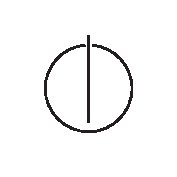
\includegraphics[width=2.4cm]{tum-info-logo}
\end{center}

\newpage

%%%%%%%%%%%%%%%%%%%%%%%%%%%%%%%
% Rückseite Deckblatt

\thispagestyle{empty}
\cleardoublepage

%%%%%%%%%%%%%%%%%%%%%%%%%%%%%%%
% Erste Seite (Titelblatt)

\thispagestyle{empty}

\begin{center}

    
\includegraphics[width=3cm]{tum-logo}\\
    \vspace{.5cm}
    {\Large \sc Technische Universität München}\\


    \vspace{.5cm}

    {\huge \sc Fakultät für Informatik\\[1mm]}


    \vspace{1cm}

    {\Large \textbf{Diplomarbeit in Informatik}}\\ % oder SEP etc.

% Thema bzw. Titel der Arbeit  (In der Sprache, in der die Arbeit verfasst wurde)
    \vspace{1.5cm}
    {\huge \textbf{Ein Lorem-Rahmenwerk}}\\ % bei langen Titeln ggf. Schriftgröße herunter setzen
    \vspace*{3mm}
    {\huge \textbf{für Ipsum-Systeme}}\\
    \vspace*{3mm}
    {\huge \textbf{-- ein Dolor-Ansatz}}\\

% die englische bzw. deutsche Entsprechung des Titels
    \vspace{1cm}
    {\huge \textbf{A Lorem Framework}}\\ % bei langen Titeln ggf. Schriftgröße herunter setzen
    \vspace*{3mm}
    {\huge \textbf{for Ipsum Systems}}\\
    \vspace*{3mm}
    {\huge \textbf{-- a Dolor Approach}}\\
    \vspace{1cm}

    \parbox{1cm}{
      \begin{large}
        \begin{tabbing}
          Bearbeiter: \hspace{1.5cm}
            \=Vorname Nachname\\[2mm]
    Aufgabensteller: \>Prof. Dr. Dieter Kranzlmüller\\[2mm]
    Betreuer: \>MNM-Team-Betreuer 1\\ % alphabetische Reihenfolge (Nachname)
    \>MNM-Team-Betreuer 2\\
    \>Externer Betreuer 1 (Firma)\\[5mm]
    Abgabedatum: \> 7. Juli 2077\\
        \end{tabbing}
      \end{large}
    }\\

    \vspace{.3cm}

    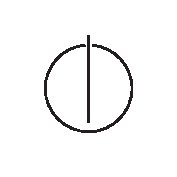
\includegraphics[width=2.4cm]{tum-info-logo}

\end{center}
 % Titelblätter TUM - auskommentiert lassen falls LMU-Arbeit
    \thispagestyle{empty}
    \cleardoublepage
    %
% LaTeX-Rahmen für Arbeiten am Lehrstuhl Hegering
%
% Harald Roelle, 2001, 2002
%
% basierend auf Arbeiten von Helmut Reiser, Boris Gruschke und Stephen Heilbronner
%

\newpage

\thispagestyle{empty}

\begin{large}

\vspace*{2cm}

\noindent
Hiermit versichere ich, dass ich die vorliegende Masterarbeit
selbst\"andig verfasst und keine anderen als die angegebenen Quellen
und Hilfsmittel verwendet habe.

\vspace{2cm}

\noindent
M\"unchen, den 19. M\"arz 2019

\vspace{3cm}

\hspace*{7cm}%
\dotfill\\
\hspace*{8.5cm}%
\textit{(Unterschrift des Kandidaten)}

\end{large}
 % Erklärung (Arbeit selbstständig verfasst) - auskommentieren falls TUM-Arbeit
%    \begin{large}

\vspace*{2cm}
\noindent
Ich versichere, dass ich diese Diplomarbeit % (bzw. Master's Thesis)
selbständig verfasst und nur die angegebenen Quellen und Hilfsmittel verwendet habe.

\vspace{2cm}

\noindent
München, den 7. Juli 2077

\vspace{3cm}

\hspace*{7cm}%
\dotfill\\
\hspace*{8.5cm}%
\textit{(Unterschrift des Kandidaten)}

\end{large}
 % Erklärung (Arbeit selbstständig verfasst) - auskommentiert lassen falls LMUArbeit
    \thispagestyle{empty}
    \cleardoublepage
    \vspace*{2cm}

\begin{center}
    \textbf{Abstract}
\end{center}

\vspace*{1cm}

\begin{comment}
%\noindent When deploying realtime AI applications, a crucial aspect is the decision whether to deploy the underlying deep learning models on edge devices or on a cloud-backend.
%For the deployment of a model various things need to be considered, most importantly accuracy and inference time, but also energy consumption, memory consumption, throughput and retraining
\noindent When deploying real-time AI applications, a crucial aspect is the decision whether to deploy the underlying deep learning models on edge devices or on a cloud-backend.
For the model inference various things need to be considered, among other things preprocessing, computational demands,
specialized hardware (GPU, TPU, neuromorphic co-processors, FPGA),
network latencies and energy consumption. Most of these aspects depend on both the model as well as the environment where the model is deployed. 
In order to help with the optimal selection of cloud and edge inference to achieve real-time AI, this thesis proposes a performance model characterising the deployment of a deep learning model and the resulting trade-offs.
Based on this performance model, the most essential trade-offs of the different deployment options get demonstrated by conducting multiple experiments using image classification as a use case. After the evaluation of these experiments, recommendations for the deployment are proposed.




When deploying real-time AI applications on edge devices, a crucial aspect is the decision whether to deploy the underlying deep learning models on edge devices or a cloud-backend.
While edge computing is often characterized by a lack of computational power and therefore struggles to provide a high throughput of predictions at a low-latency, outsourcing the inference to a cloud-backend raises concerns regarding security and reliability.
Although low-latencies and throughput are the most critical inference performance metric for real-time applications on edge devices, other metrics like CPU usage, data-, memory- or energy-consumption are affected by both cloud and edge inference and hence vital for the model deployment to consider.

%All these performance metrics are mainly affected by four factors: The model architecture, hardware, inference framework and the shape of the inference input.
%Significant research is being done in all these areas influencing the deployment question, resulting in the release of optimized frameworks (TensorFlow Lite, NNAPI, TensorFlow Serving), hardware accelerators (GPU, TPU, neuromorphic co-processors, FPGA) and models dedicated for edge devices (MobileNet).
-----------------------------------------------------------------------------
\end{comment}




\noindent In the wake of the recent achievements in the topic of deep learning, the number of possible real-time AI applications on edge devices has exploded.
However, the deployment of these model is often difficult as edge computing is often characterized by a lack of computational power and therefore struggles to provide high inference throughput at low latencies.
Outsourcing the inference to a cloud-backend can provide more computational power, but raises concerns regarding security and reliability. 
Although latency and throughput are the most critical inference performance metrics for real-time applications on edge devices, other metrics like CPU usage, data-, memory- or energy-consumption are affected by both cloud and edge inference and hence vital for the model deployment to consider.

In order to help with the optimal selection of cloud and edge inference to achieve real-time AI, this thesis proposes a methodology for performance evaluation of deep learning inference.
By instantiating this methodology we get a better system understanding of deep learning inference including benchmarks of the above-mentioned performance metrics.

To generate these benchmarks we use image classification as use case, supported by real-world workloads and hardware components and frameworks.
The evaluation of these benchmarks show, that edge inference can outperform cloud inference, given the right circumstances.
These include optimization of deep learning model architectures, utilization of optimized inference frameworks and minimization of preprocessing.


Based on these benchmarks we then develop a performance model, predicting the optimal deployment solution for a given system configuration, using multiple linear regression.
Finally, we utilize the gained system understanding to create a generic decision model that supports the deployment process for deep learning inference.



%%TODO add results 
%%Results: edge better for small models, cloud for large models; large batch sizes not viable at the edge, impact of preprocessing
%Our results show that edge devices can deliver better inference performance than cloud inference would for small models, but for large models cloud inference is still the preferred option for high performance, at least for the moment.
%Another key lesson is the impact of preprocessing on inference performance. The amount of preprocessing should be minimized

%proposes a performance model characterising the deployment of deep learning models and the resulting performance trade-offs.
 % Abstract
    \thispagestyle{empty}
    %%\addtocontents{toc}{\protect\enlargethispage{\baselineskip}}
    \tableofcontents % Inhaltsverzeichnis

% ---------------------------------------------------------------
\mainmatter % die eigentliche Arbeit

    \chapter{Introduction}


%%ADD: android application
The last few years have been marked by tremendous successes in the field of deep learning.
Deep learning models have become very accurate at complex tasks such as image classification, object detection or natural language processing. 
With this success, the number of possible AI applications using these models increased rapidly, especially on edge devices such as cars, smartphones or IoT devices.
These applications have a broad range from industry to scientific applications and often have in common that they need predictions at real-time to unfold their full potential.
This process of getting predictions from a trained deep learning model for a given input, for example getting the probability that a given image contains a cat, is called inference.
The strength of deep learning models is to generate accurate and reliable predictions, without human help, but if the inference takes too long or consumes too many other resources, the model becomes infeasible for the usage in real-time AI applications.
Therefore it is critical to ensure that inference can be done in real-time.

However, as the accuracy of these models has risen, the computational demand has also due to the models increasing architectural size.
This has taken a toll on the performance of these models apart from the accuracy, in particular on performance aspects such as inference latency, memory consumption, energy consumption, CPU usage and throughput. 
While inference time and throughput are the essential metrics to ensure real-time AI, memory usage, energy consumption and CPU usage are also crucial in order to avoid that the inference consumes the majority of the system resources.
This is a concern especially for latency-sensitive AI application on edge devices, as edge computing often is constrained by limited computational power. 
That is why the question arose whether a deep learning model can be deployed to the edge or has to be deployed to cloud-backend where more computational power is available.
However, edge inference, and edge computing in general, offers many advantages compared to cloud computing such as low-latencies, improved reliability and fewer privacy concerns\cite{Mor:2018:EC:3305263.3313377}.
Therefore edge deployment should be the preferred option for deep learning inference if the desired inference performance can be achieved.


To support users with the optimal selection of deployment for deep learning inference, this thesis introduces a methodology for the performance evaluation of deep learning inference, applicable to both edge and cloud inference.
The goal of this performance evaluation is a better understanding of deep learning inference, helping us to design a performance model predicting the optimal deployment solution, as well as a generic decision model for the deployment of deep learning models.
To achieve this goal this methodology presents a systematic approach towards the performance evaluation for deep learning inference, started by the definition of the problem space and performance metrics, followed by the design of a use case using real-life workloads and infrastructure. This use case is then executed on a self-developed benchmark system to create benchmarks.
These benchmarks then can be used for evaluation, resulting in a performance model as well as a decision model. Therefore these benchmarks contribute to a better understanding of deep learning inference.

This methodology then gets instantiated step by step, started by the analysis of the problem space.
We identified four factors influencing the inference performance: the hardware specification of the deployment environment, the architecture of the deep learning model and the framework responsible for performing the inference operations of the deep learning model on the hardware components. The fourth factor is the inference input, on which the inference is performed on, since preprocessing of these inputs is often necessary and thus impacting the inference performance.

There exists a rich variety of different neural network types, with the most popular being convolutional neural networks(CNNs) and recurrent neural networks(RNNs).
Many of these models use unique operators with different impact on inference performance.
Since it is not feasible to benchmark all these different network types, this thesis will use CNNs as an exemplary use case, specifically image classification models classifying the contents of a given input image.

This rich variety of configurations also applies to the hardware aspects, where in addition to better CPUs and GPUs a rising number of specific accelerators such as TPUs, neuromorphic co-processors and FPGAs have been developed for both edge and cloud.
For the benchmarks, we will use the OnePlus 6T, a state of the art smartphone, as our edge device and a server with an Nvidia Tesla P100 as the cloud-backend.

TensorFlow Serving and TensorFlow Lite, both open-source, will serve as the example inference frameworks for these benchmarks, as they support the deployment of deep learning models to a cloud-backend (TensorFlow Serving) or directly to edge devices (TensorFlow Lite). These frameworks support many of the above mentioned hardware accelerators and provide optimized operators used by image classification models.

Based on this infrastructure and workload we then design and implement an Android benchmark system simulating a real-time AI application.
We then execute this system to generate benchmarks, which we will then analyze for for better understanding of deep learning inference. Afterwards the benchmarks will be used to create a performance model as well as a decision model.
This performance model will predict the optimal deployment solution for a given system configuration.

Another aspect, aside from the actual inference, is the preprocessing step, which is needed to transform the input into the format required by the model. 
In the case of CNNs these steps often consist of image resizing and normalization.
Since this step is vital for the inference, our benchmarks will also include a study on the impact of preprocessing of various workload sizes, in our case images, aside from the actual inference.

\section{Structure of the Thesis}
The rest of this thesis is structured as follows: 
Chapter \ref{chap:fundamentels} gives a brief overview of the fundamentals of deep learning and model deployment, both at the edge and the cloud, as this understanding is crucial for evaluating the inference performance later on.
Chapter \ref{chap:relatedWork} provides an outline and evaluation of existing related work on this topic. 
Next, we propose a methodology towards a systematic approach towards performance evaluation of deep learning inference, starting by analyzing the problem space and ending with a performance as well as a decision model supporting the optimal selection of deep learning deployment.
Chapter \ref{chap:experiments} deals with the step by step instantiation of the defined methodology.
Finally, this thesis closes with a conclusion and possible future work topics inspired by this thesis.

    \chapter{Fundamentals}
\label{chap:fundamentels}
In this chapter we briefly cover the fundamentals of deep learning models and their deployment on edge devices and cloud-backends for inference purposes.
These fundamentals are needed to understand the problem space of this thesis.


%The inference performance of a deep learning model is mainly affected by three factors, the architecture of the deep learning model itself, the hardware environment where it gets deployed and the framework performing the operations of the model on the hardware environment.
%These three aspect are covered in this section.

\section{Deep Learning}
%%Bisschen genauer was deep learning input output...
%Einfluss auf inference latency an memory?
This section gives a brief, but nowhere complete overview of the deep learning field. We will focus on the basic structures and intuition behind deep learning models, as a comprehensive analysis would go beyond the scope of this thesis.

%Deep learning are a subclass of neural networks, which differ from normal neural network by having large architectures in the form of layers, leading to high computational demands.
Neural networks try make a prediction $\mathbf{\Hat{Y}}$, for a  given an input $\mathbf{X}$, that is as close as possible to the underlying ground truth $\mathbf{Y}$. 
Deep learning is a subclass of neural networks.
The difference between neural networks and deep learning networks is the number of layers and hidden units. Deep learning models consist of many hidden layers and hidden units leading to deep architectures.
These deep architectures with often millions of parameters lead to a significant increase in computational power for both training and inference.
%While for simple linear regression model with a single variable a single computation
% ground through Y and the net predictions Y hat
\begin{figure}[!htb]
%%bild mit simpler architecture? Bild->conv->pool->flatten->dense-> output
    \centering
    \resizebox{.8\linewidth}{!}{\def\layersep{2.5cm}
\begin{tikzpicture}[shorten >=1pt,->,draw=black!50, node distance=\layersep]
    \tikzstyle{every pin edge}=[<-,shorten <=1pt]
    \tikzstyle{neuron}=[circle,fill=black!25,minimum size=17pt,inner sep=0pt]
    \tikzstyle{input neuron}=[neuron, fill=gray!50];
    \tikzstyle{output neuron}=[neuron, fill=gray!50];
    \tikzstyle{hidden neuron}=[neuron, fill=black!50];
    \tikzstyle{annot} = [text width=4em, text centered]

    % Draw the input layer nodes
    \foreach \name / \y in {1,...,4}
    % This is the same as writing \foreach \name / \y in {1/1,2/2,3/3,4/4}
        \node[input neuron, pin=left:$x_\y$] (I-\name) at (0,-\y) {};

    % Draw the hidden layer nodes
    \foreach \name / \y in {1,...,5}
        \path[yshift=0.5cm]
            node[hidden neuron] (H-\name) at (\layersep,-\y cm) {};
    % Draw the hidden layer nodes
    \foreach \name / \y in {2,...,4}
        \path[yshift=0.5cm]
            node[hidden neuron] (H2-\name) at (\layersep+2.5cm,-\y cm) {};
    % Draw the hidden layer nodes
    \foreach \name / \y in {1,...,5}
        \path[yshift=0.5cm]
            node[hidden neuron] (H3-\name) at (\layersep+5cm,-\y cm) {};
    % Draw the output layer node
    \node[output neuron,pin={[pin edge={->}]right:$\mathbf{\hat{Y}}$}, right of=H3-3] (O) {};

    % Connect every node in the input layer with every node in the
    % hidden layer.
    \foreach \source in {1,...,4}
        \foreach \dest in {1,...,5}
            \path (I-\source) edge (H-\dest);
            
    \foreach \source in {1,...,5}
        \foreach \dest in {2,...,4}
            \path (H-\source) edge (H2-\dest);
    \foreach \source in {2,...,4}
        \foreach \dest in {1,...,5}
            \path (H2-\source) edge (H3-\dest);

    % Connect every node in the hidden layer with the output layer
    \foreach \source in {1,...,5}
        \path (H3-\source) edge (O);

    % Annotate the layers
    \node[annot,above of=H-1, node distance=1cm] (hl) {Hidden layer};
    \node[annot,above of=H2-2, node distance=2cm] (hl2) {Hidden layer};
    \node[annot,above of=H3-1, node distance=1cm] (hl3) {Hidden layer};
    \node[annot,left of=hl] {Input layer};
    \node[annot,right of=hl3] {Output layer};
\end{tikzpicture}}
    \caption{Simple neural network with 4 inputs, 3 hidden layers and 1 output.}
    \label{fig:simpleNN}
\end{figure}

Figure \ref{fig:simpleNN} shows the structure of a simple neural network with input $\mathbf{X}$ and output $\mathbf{\Hat{Y}}$, where $\mathbf{X}$ is a vector of size four, meaning the neural network takes four features as its input. 
The output $\mathbf{\Hat{Y}}$ for this example is a vector of only size one, hence the network predicts one value.
Between the input and output of this example network lay three fully connected hidden layers, also called dense layers, with five, three and again five hidden units.
Each of these hidden layers has a weight matrix $\mathbf{W\in\mathbb{R}^{m\times n}}$, where $\mathbf{m}$ is the number of hidden units and $\mathbf{n}$ the number of hidden units in the previous layer.
This weight matrices are needed to compute the state of each hidden layer by calculating the weighted sum of all its inputs.
For example, the state of the first hidden layer is calculated by multiplying $\mathbf{W_1X}$, where $\mathbf{W_1}$ is the weight matrix of layer $1$ and $\mathbf{X}$ the output of the previous layer, in this case, the input layer.
To calculate  $\mathbf{\Hat{Y}}$ in the output layer using $\mathbf{W_O}$, all previous states need to calculated consecutively. 
This chain of calculations needed to get from input $\mathbf{X}$ to output $\mathbf{\Hat{Y}}$ is also called forward-propagation because the values of the input vector get passed through all layers by multiplication.
For the example network in figure \ref{fig:simpleNN} all computations can be seen in equation \ref{eq:1}, with the shapes of all input/output vectors and weight matrices depicted in equation \ref{eq:2}.

\begin{equation} \label{eq:1}
\begin{gathered}
\mathbf{\hat{Y}(X)} = \mathbf{W_O(W_3(W_2(W_1X)))}
\end{gathered}
\end{equation}


\begin{equation} \label{eq:2}
\begin{gathered}
\mathbf{X} = \begin{bmatrix}
           x_{1} \\
           x_{2} \\
           x_{3} \\
           x_{4}
         \end{bmatrix},
\mathbf{W_1} = \begin{bmatrix}
           w_{11} & w_{12}& w_{13}& w_{14}\\
           w_{21} & w_{22}& w_{23}& w_{24} \\
           w_{31} & w_{32}& w_{33}& w_{34} \\
           w_{41} & w_{42}& w_{43}& w_{44} \\
           w_{51} & w_{52}& w_{53}& w_{54} 
         \end{bmatrix},
\mathbf{W_2} = \begin{bmatrix}
           w_{11} & w_{12}& w_{13}& w_{14}& w_{15}\\
           w_{21} & w_{22}& w_{23}& w_{24}& w_{25} \\
           w_{31} & w_{32}& w_{33}& w_{34}& w_{35} 
         \end{bmatrix},\\ \\
\mathbf{W_3} = \begin{bmatrix}
           w_{11} & w_{12}& w_{13}\\
           w_{21} & w_{22}& w_{23} \\
           w_{31} & w_{32}& w_{33} \\
           w_{41} & w_{42}& w_{43} \\
           w_{51} & w_{52}& w_{53} 
         \end{bmatrix},
\mathbf{W_O} = \begin{bmatrix} w_{11} & w_{12}& w_{13}& w_{14}& w_{15} \end{bmatrix},
\mathbf{\hat{Y}} = \begin{bmatrix} y_1 \end{bmatrix}
%\hat{Y} = (1\times5)(5\times3)(3\times5)(5\times4) (4\times1) = (1\times5)(5\times3)(3\times5)(5\time1) = (1\times5)(5\times3)(3\times1) = (1\times5)(5\times1) = 1
\end{gathered}
\end{equation}

For the sake of simplicity the example does not use activation functions $\mathbf{\sigma}$ (e.\,g. ReLU) and biases $\mathbf{b}$, which would usually be used in practice in the form of $\mathbf{\sigma(WX+b)}$ instead of $\mathbf{WX}$.
Activation functions are needed to decide if a neuron (hidden unit) fires or not as well as minimizing the risk of exploding/vanishing gradients.
%beispielrechnung für das nn


This simple network only contains three hidden layers with at most five hidden layers and thus 45 parameters in total, but in practice state of the art deep learning models often contain millions of parameters. 
The forward propagation of such models often causes the need for more than $1$ GFLOPS, leading to high computational demands for real-time AI applications.

%15+5+15+20 = 45 parameters
%large network >10 000 000 param

There are many different operators and network architectures, all with different computational demands, thus making performance prediction very complex.
Since we will use image classification as a use case for the benchmarks in section \ref{chap:experiments}, we will now present the basics of Convolutional Neural Networks, which are used for this use case.

\paragraph{Convolutional Neural Network}
This specific class of neural network achieved wide success in the field of image classification and object detection.
The strength of Convolutional Neural Networks (CNN) is the ability to extract features like complex shapes or colour patterns from images. Thus this network is particularly suitable for image classification.
%Abschnitt über convolutions und pooling?

Image classification networks classify the contents of an image by outputting classes for the image with respective confidence levels, for example, how likely an animal on a picture represents a cat.
A simple architecture for this classification task can be seen in figure \ref{fig:simpleCNN}.
The network expects input images as a three-dimensional tensor $h\times w\times c$, where $h$ and $w$ are the fixed height and width of the image and $c$ is the number of channels, which in most cases is $3$ for the $3$ \emph{RGB} channels.
An image needs to be preprocessed to match these shape specifications before feeding it to the network.
The fundamental building blocks of CNNs are multiple convolution layers, which extract features from the images. The first convolutional extract simple features like edges from the image, while the later convolutional layers combine these simple features to complex shapes like rectangles.
To reduce the spatial dimension of the feature maps, outputted by the convolution, a popular layer type added to CNNs are pooling layers.
After extracting all features are extracted, the resulting tensor gets flattened to a one-dimensional tensor before getting reaching one or more fully connected layers.
The last fully connected layer contains the output of the network, in this case, confidence levels for predefined labels (e.\,g. $80$\% cat).  


\begin{figure}[!htb]
%%bild mit simpler architecture? Bild->conv->pool->flatten->dense-> output
    \centering
    \resizebox{.95\linewidth}{!}{

\tikzset{every picture/.style={line width=0.75pt}} %set default line width to 0.75pt        

\begin{tikzpicture}[x=0.75pt,y=0.75pt,yscale=-1,xscale=1]
%uncomment if require: \path (0,360.3333282470703); %set diagram left start at 0, and has height of 360.3333282470703

%Shape: Rectangle [id:dp05899425458959939] 
\draw  [color={rgb, 255:red, 160; green, 160; blue, 160 }  ,draw opacity=1 ][fill={rgb, 255:red, 160; green, 160; blue, 160 }  ,fill opacity=1 ][line width=1.5]  (760,203) -- (776.83,203) -- (776.83,213.33) -- (760,213.33) -- cycle ;
%Image [id:dp4912524236296907] 
\draw (66.08,133.08) node  {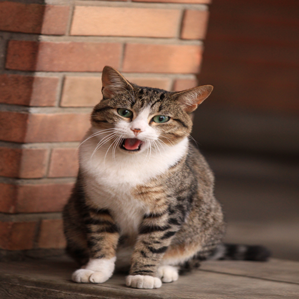
\includegraphics[width=79.62pt,height=79.62pt]{Bilder/European_cat_02_299.png}};
%Shape: Cube [id:dp48120440402395137] 
\draw  [fill={rgb, 255:red, 255; green, 255; blue, 255 }  ,fill opacity=1 ] (189,92.33) -- (149,52.33) -- (141,52.33) -- (141,171.33) -- (181,211.33) -- (189,211.33) -- cycle ; \draw   (141,52.33) -- (181,92.33) -- (189,92.33) ; \draw   (181,92.33) -- (181,211.33) ;
%Shape: Cube [id:dp1963658989292536] 
\draw  [fill={rgb, 255:red, 232; green, 232; blue, 232 }  ,fill opacity=1 ] (280,111.4) -- (241.94,73.33) -- (196,73.33) -- (196,170.27) -- (234.06,208.33) -- (280,208.33) -- cycle ; \draw   (196,73.33) -- (234.06,111.4) -- (280,111.4) ; \draw   (234.06,111.4) -- (234.06,208.33) ;
%Shape: Cube [id:dp9995029386851741] 
\draw  [fill={rgb, 255:red, 155; green, 155; blue, 155 }  ,fill opacity=1 ] (406,138.31) -- (377.08,109.4) -- (298,109.4) -- (298,171.48) -- (326.92,200.4) -- (406,200.4) -- cycle ; \draw   (298,109.4) -- (326.92,138.31) -- (406,138.31) ; \draw   (326.92,138.31) -- (326.92,200.4) ;
%Shape: Cube [id:dp47292096524654625] 
\draw  [fill={rgb, 255:red, 155; green, 155; blue, 155 }  ,fill opacity=1 ] (665.17,154.88) -- (648.62,138.33) -- (565,138.33) -- (565,173.85) -- (581.54,190.4) -- (665.17,190.4) -- cycle ; \draw   (565,138.33) -- (581.54,154.88) -- (665.17,154.88) ; \draw   (581.54,154.88) -- (581.54,190.4) ;
%Shape: Rectangle [id:dp9622310163181891] 
\draw   (736,94.33) -- (736,246.33) -- (717.17,246.33) -- (717.17,94.33) -- cycle ;
%Shape: Rectangle [id:dp3888373908322751] 
\draw   (778,104.33) -- (778,236.33) -- (759,236.33) -- (759,104.33) -- cycle ;
%Shape: Rectangle [id:dp6404657361959689] 
\draw  [fill={rgb, 255:red, 0; green, 0; blue, 0 }  ,fill opacity=1 ] (760,132) -- (776.83,132) -- (776.83,142.33) -- (760,142.33) -- cycle ;
%Straight Lines [id:da7775179037387632] 
\draw    (783.17,137.33) -- (806.17,137.33) ;
\draw [shift={(808.17,137.33)}, rotate = 180] [fill={rgb, 255:red, 0; green, 0; blue, 0 }  ][line width=0.75]  [draw opacity=0] (8.93,-4.29) -- (0,0) -- (8.93,4.29) -- cycle    ;

%Shape: Cube [id:dp25140851319063606] 
\draw  [fill={rgb, 255:red, 232; green, 232; blue, 232 }  ,fill opacity=1 ] (534.17,145.87) -- (510.63,122.33) -- (433,122.33) -- (433,172.86) -- (456.53,196.4) -- (534.17,196.4) -- cycle ; \draw   (433,122.33) -- (456.53,145.87) -- (534.17,145.87) ; \draw   (456.53,145.87) -- (456.53,196.4) ;
%Straight Lines [id:da07111443875380252] 
\draw    (189.17,135.33) -- (224.17,139.33) ;


%Straight Lines [id:da7555086779952114] 
\draw    (189.17,150.33) -- (224.17,139.33) ;


%Straight Lines [id:da6920716028952918] 
\draw    (190.17,124.33) -- (224.17,139.33) ;


%Straight Lines [id:da20921164719439567] 
\draw    (279.17,153.33) -- (314.17,157.33) ;


%Straight Lines [id:da5314884265558493] 
\draw    (279.17,168.33) -- (314.17,157.33) ;


%Straight Lines [id:da9607824424543641] 
\draw    (280.17,142.33) -- (314.17,157.33) ;


%Straight Lines [id:da22420538027937398] 
\draw    (405.17,162.33) -- (440.17,166.33) ;


%Straight Lines [id:da8064502796691653] 
\draw    (405.17,177.33) -- (440.17,166.33) ;


%Straight Lines [id:da9671090843658954] 
\draw    (406.17,151.33) -- (440.17,166.33) ;


%Straight Lines [id:da6406059045755481] 
\draw    (533.17,166.33) -- (568.17,170.33) ;


%Straight Lines [id:da9716418537016991] 
\draw    (533.17,181.33) -- (568.17,170.33) ;


%Straight Lines [id:da548327903780097] 
\draw    (534.17,155.33) -- (568.17,170.33) ;


%Straight Lines [id:da32303530471950226] 
\draw    (665.17,171.33) -- (715.17,171.33) ;
\draw [shift={(717.17,171.33)}, rotate = 180] [fill={rgb, 255:red, 0; green, 0; blue, 0 }  ][line width=0.75]  [draw opacity=0] (8.93,-4.29) -- (0,0) -- (8.93,4.29) -- cycle    ;

%Straight Lines [id:da4465574217797632] 
\draw    (735.17,171.33) -- (757.17,171.33) ;
\draw [shift={(759.17,171.33)}, rotate = 180] [fill={rgb, 255:red, 0; green, 0; blue, 0 }  ][line width=0.75]  [draw opacity=0] (8.93,-4.29) -- (0,0) -- (8.93,4.29) -- cycle    ;

%Straight Lines [id:da9780199762846196] 
\draw    (784.17,209.33) -- (807.17,209.33) ;
\draw [shift={(809.17,209.33)}, rotate = 180] [fill={rgb, 255:red, 0; green, 0; blue, 0 }  ][line width=0.75]  [draw opacity=0] (8.93,-4.29) -- (0,0) -- (8.93,4.29) -- cycle    ;


% Text Node
\draw (840,135) node  [align=left] {Cat \ $\displaystyle 0.8$};
% Text Node
\draw (185,219) node  [align=left] {$\displaystyle c$};
% Text Node
\draw (153,199) node [rotate=-45.72] [align=left] {$\displaystyle w$};
% Text Node
\draw (131,111) node [rotate=-269.52] [align=left] {$\displaystyle h$};
% Text Node
\draw (235,54) node  [align=left] {Convolution};
% Text Node
\draw (339,89) node  [align=left] {Pooling};
% Text Node
\draw (609,119) node  [align=left] {Pooling};
% Text Node
\draw (724,72) node  [align=left] {Dense};
% Text Node
\draw (770,86) node  [align=left] {Dense};
% Text Node
\draw (689,153) node  [align=left] {Flatten};
% Text Node
\draw (477,103) node  [align=left] {Convolution};
% Text Node
\draw (145,35) node  [align=left] {Input};
% Text Node
\draw (842,207) node  [align=left] {Dog \ $\displaystyle 0.1$};
% Text Node
\draw (70,192) node  [align=left] {{\scriptsize source: [SeL] }};


\end{tikzpicture}}
    \caption{Simple CNN for image classification}
    \label{fig:simpleCNN}
\end{figure}

%Add calculation example
\subsection{Training}
Constructing the architecture of a model is the first step, but in order to enable models to make accurate predictions, they have to be trained, which means adjusting the weights of the network. 
Since most neural networks are a type of supervised learning, training data with ground truth labels $\mathbf{Y}$ is needed for the training.
This training is done with forward- and back-propagation, where one or more samples of the training set are forward propagated through the network until reaching the output layer. Afterwards, the $Loss\mathbf{(Y,\Hat{Y})}$ can be calculated, which measures the difference between the prediction $\mathbf{\Hat{Y}}$ and the ground truth $\mathbf{Y}$.

To optimize the network, the loss needs to be minimized, meaning that the difference between prediction and ground truth is as small as possible and thus the accuracy as high as possible.
Since there is no closed form solution to find this minimum most of the time, neural network use gradient descent, specifically back-propagation, to minimize the loss in an iterative process.
Given the loss of the network, the gradients of all weights in the network can be computed and afterwards the weights can be updated using a learning rate in respect to the gradient and learning rate.

This process of forward- and back-propagation is repeated for all sample in the training data set multiple times until the minimum loss is reached and therefore the highest possible accuracy.

\subsection{Inference}
%only forward prop

After the model is trained it is ready to be deployed in a production environment, where it can serve its predictions to an application. This process of forward propagating the input through a neural network, performing all computational operations defined in the model, resulting in an output/prediction, is called inference.

However, since models often require the input to be of a specific shape and the input given by an application often does not match that shape, a preprocessing step is often needed before the actual inference can be performed.
This preprocessing and inference process can also be seen in figure \ref{fig:InfProcess}.
%%Add visualization of input here
%%die dann im deployment wieder aufgreifen
\begin{figure}[H]
\centering


\tikzset{every picture/.style={line width=0.75pt}} %set default line width to 0.75pt        

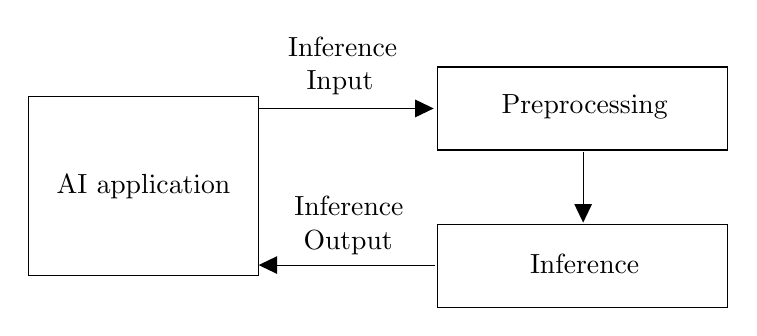
\begin{tikzpicture}[x=0.75pt,y=0.75pt,yscale=-1,xscale=1]
%uncomment if require: \path (0,300); %set diagram left start at 0, and has height of 300

%Shape: Rectangle [id:dp7725979857917211] 
\draw  [fill={rgb, 255:red, 255; green, 255; blue, 255 }  ,fill opacity=1 ] (262,80) -- (402,80) -- (402,120) -- (262,120) -- cycle ;
%Shape: Rectangle [id:dp3208391580840302] 
\draw  [fill={rgb, 255:red, 255; green, 255; blue, 255 }  ,fill opacity=1 ] (262,156) -- (402,156) -- (402,196) -- (262,196) -- cycle ;
%Straight Lines [id:da5532652572924177] 
\draw    (175.93,99.98) -- (258.29,99.98) ;
\draw [shift={(260.29,99.98)}, rotate = 180] [fill={rgb, 255:red, 0; green, 0; blue, 0 }  ][line width=0.75]  [draw opacity=0] (8.93,-4.29) -- (0,0) -- (8.93,4.29) -- cycle    ;

%Straight Lines [id:da9616587358279531] 
\draw    (332.29,121) -- (332.29,152.98) ;
\draw [shift={(332.29,154.98)}, rotate = 270] [fill={rgb, 255:red, 0; green, 0; blue, 0 }  ][line width=0.75]  [draw opacity=0] (8.93,-4.29) -- (0,0) -- (8.93,4.29) -- cycle    ;

%Straight Lines [id:da0888724954521467] 
\draw    (260.93,175.43) -- (177.93,175.43) ;
\draw [shift={(175.93,175.43)}, rotate = 360] [fill={rgb, 255:red, 0; green, 0; blue, 0 }  ][line width=0.75]  [draw opacity=0] (8.93,-4.29) -- (0,0) -- (8.93,4.29) -- cycle    ;

%Shape: Rectangle [id:dp6392688617606377] 
\draw  [fill={rgb, 255:red, 255; green, 255; blue, 255 }  ,fill opacity=1 ] (64.93,94.43) -- (175.93,94.43) -- (175.93,180.43) -- (64.93,180.43) -- cycle ;

% Text Node
\draw (333,99) node  [align=left] {Preprocessing};
% Text Node
\draw (333,175) node  [align=left] {Inference};
% Text Node
\draw (120.43,137.43) node  [align=left] {AI application};
% Text Node
\draw (216.43,79.43) node  [align=left] {Inference\\ \ \ Input};
% Text Node
\draw (219.43,156.43) node  [align=left] {Inference\\ \ Output};


\end{tikzpicture}
\caption{Visualization of the inference process for AI applications, including preprocessing.}
\label{fig:InfProcess}
\end{figure}
Note that the architecture of the inference model is often slightly different from the training model, as some operators are only needed for the training process and are thus removed for inference (e.\,g. dropout).





\subsection{Model Optimization}
There are various methods to optimize the architecture of a deep learning model to achieve better inference performance.
The difficulty in optimizing deep learning models is to improve inference performance while not loosing accuracy.
One technique is quantization, which we will briefly introduce in the following paragraph.
\subsubsection{Quantization}
\label{chap:quant}
Quantization is a model optimization technique that often trades in model precision for better inference latencies, memory consumption during inference and model sizes.
Quantization describes the process of reducing the "precision representations of weights and, optionally, activations" \cite{tfLiteQuant} from floating point precision to for example 8-bit.
The weights/activations are either quantized after training the model with floats (Post Training Quantization), or the model is trained with quantized weights/activations from the start (Quantization Aware Training). In the paper "Quantizing deep convolutional networks for
efficient inference"\cite{Quantizing} Krishnamoorthi performed a study on these techniques with the following results:
8-bit quantization can lead to a model size reduction by a factor of 4, a 2-3x latency speedup on CPUs and DSPs, while reducing the model accuracies by 1\%.


\section{Deployment of Deep Learning Models}
Deep learning deployment describes the process of deploying a (trained) machine learning model to a production environment for inference purposes. 

%%Write more here
There can be differentiated between two different deployment methods. The first one is deploying the model directly to edge devices, while the second outsources the model to a cloud-backend, where the inference is performed, and the prediction is then sent back to the edge device.
\subsection{Edge Deployment}
Edge deployment describes the process of deploying deep learning models to edge devices such as mobile devices like smartphones, cars or Raspberry Pis.
These edge devices are characterized by offering a limited amount of computational power as well as limited energy.
This limited power often stands in contrast to the performance demands caused real-time AI applications using deep learning models.
Despite its limits, edge deployment also has some advantages, particularly in reliability and security. 
For example in the case of image classification images are needed for the inference, which often contain sensible information and thus raise data privacy/security concerns.
Therefore edge deployment should be the preferred choice if the inference performance is sufficient for the use case of real-time AI applications.

In order to increase this performance, various accelerators like better GPUs, TPUs or other dedicated neural network hardware components have been developed for edge devices.
%%mention NNAPI here?



\subsection{Cloud Deployment}
While the breakthroughs in deep learning are very interesting for AI applications on edge devices, the computational demand needed for edge deployment often exceeds the available power to be viable.
That is why the option of outsourcing the models to a cloud-backend has become a popular solution in recent years.
Cloud-backends offer a large amount of computational power, especially suitable for deep learning in the form large numbers of GPUs and TPUs.


The big downside of cloud-based inference is the needed network connection, in particular for edge devices such as cars, where a reliable network connection can often not be guaranteed for example in rural areas. Hence this is not a viable solution for applications like autonomous driving, where continuous and reliable predictions from deep learning models as critical for the applications feasibility.

While for the edge deployment necessary preprocessing steps are always done on the edge, for the case of cloud inference there are two possibilities. Either the input data is preprocessed to the correct shape at the edge before getting sent to the cloud-backend, or the input is sent un-preprocessed to the cloud. 
In the latter case, the input gets preprocessed on the cloud. 
This can be justified by the same reasons as for the cloud inference, more computational power for intensive preprocessing.
Although slow network connection could diminish the speedup gained by the larger computational power, since non preprocessed input are most of the times larger in payload size and therefore more data has to be sent to the server, resulting in the need of faster network connections to achieve the same network latency as a preprocessed input would.
However in the case of compressed inputs as for example \emph{JPEG} images, if the \emph{JPEG} and the preprocessed image have the same input size, the \emph{JPEG} image could lead to faster latencies, as less data has to be sent to the server and the I/O overhead at the server is minimized, as the server has to load a smaller image into memory assuming \emph{JPEG} decoding is faster than the I/O overhead of load a larger image. 



\section{Inference Framework}
For both edge and cloud inference, the underlying inference framework is important for the inference performance since optimized model operations or support of accelerators like GPUs can lead to significant performance improvements.
New hardware components like accelerators and new deep learning operations for example in the form of new activation functions are being developed at a fast pace. Therefore a well maintained and frequently updated framework is critical for the best inference performance possible.
Another challenge is the support of the wide variety of different types of edge devices with different system architectures.

An additional factor affecting cloud inference performance is the network component, especially the impact on latency.
Thus frameworks should implement low latency protocols with small payloads for environments with constrained networks.

In this thesis, we only evaluate the inference performance of a single client sending requests to a cloud-backend, but in reality, most of the time each edge device does not have exclusive access to a cloud-backend, resulting in multiple client making inference request to a single server, possibility even at the same time.
This raises questions on how to handle multiple requests coming from multiple sources in general and specifically how to handle multiple simultaneous requests and which requests should be prioritized.

Possible solutions include combining multiple requests and performing inference of multiple requests at once by combining them into a single batch.
This approach requires a policy on how many requests to combine at most and how long the interval is where the server waits on incoming requests if the optimal batch size is not yet reached. 
While this approach can increase throughput, it often comes at the cost of increased latency, thus negatively affecting the performance of real-time AI applications at the edge.


\vspace{0.5cm}
This chapters gave an introduction to the topic of deep learning inference and the deployment of deep learning models for this inference.
This knowledge will be the base for the following chapters.
The next chapter will give an outline of related work relevant for this thesis.
%%reduce data consumption?
%%REST vs gRPC
%%cloud inference needs to support multiple client-> low latency vs throughput
%%



	\chapter{Related Work}
\label{chap:relatedWork}
This chapter will give a brief outline and evaluation of related work on the topic of performance evaluation of deep learning inference. These related paper deal with the performance evaluation of either edge or cloud inference or both of them in a comparative fashion.

%%Change title to more fitting one
%\section{Performance of Edge vs Cloud Inference}
%\subsection{Speed/accuracy trade-offs for modern convolutional object detectors}
%In \cite{DBLP:journals/corr/HuangRSZKFFWSG016} the authors provide a guide for selecting the right convolutional object detection architecture for the desirable speed/memory/accuracy. To demonstrate this trade-offs the authors test various popular models such as Inception v2, MobileNet or Resnet 101. To create the benchmarks, "a machine with 32GB RAM,
%Intel Xeon E5-1650 v2 processor and an Nvidia GeForce
%GTX Titan X GPU card \cite{DBLP:journals/corr/HuangRSZKFFWSG016} is used.


\section{Cloud-based or On-device:
An Empirical Study of Mobile Deep Inference}
Guo "evaluate[s] the inference performance of three Convolutional Neural Networks
(CNNs) using a benchmark Android application" \cite{DBLP:conf/ic2e/Guo18} for both cloud and edge inference. The hardware and frameworks used to conduct the experiments leading to this evaluation can be seen in table \ref{frameworks_hardware_1}. The three tested CNNs are image classification models (AlexNet, NIN and SqueezeNet) with an image input size of $224\times224$.
They divided the experiment in 4 steps and measure the executing time of each step: 
The model loading time (1.\,Load model), the time needed to resize the image into a $224\times224$ bitmap (2.\,Rescale bitmap), the time needed to upload the bitmap to the server in case of cloud inference (3.\,Upload bitmap) and the inference time (4.\,Compute probability).
Additional to the latencies they measured the CPU usage, battery and memory consumption during these 4 steps using Trepn Profiler.
They used 15 images in total, divided in three different image size groups ($540\times960$, $108\times1920$, $2160\times3840$) with the same 5 scaled images in each group.

After analyzing their measurements, they present the following results:
Cloud inference "exhibits substantial benefits
in terms of inference response time and mobile energy savings
over on-device inference, in this case by two orders of magnitude". As the responsible bottleneck for this conclusion they identify the model loading and inference times during edge inference.
Also it is more efficient to upload the 540x960 images directly to cloud without resizing them on the edge beforehand.


\begin{table}[H]
\centering
\caption{Hardware and inference frameworks used by \cite{DBLP:conf/ic2e/Guo18}}
\begin{tabular}{@{}lll@{}}
\toprule
 & Frameworks & Hardware \\
 \midrule
Edge & Caffe Android Lib; CNNDroid & Nexus 5 \\
Cloud & Caffe & Intel Xeon E5-2670, Nvidia Grid K520, 15GB Memory\\
\bottomrule

\end{tabular}

\label{frameworks_hardware_1}
\end{table}
%%NICHT VOLLSTÄNDIG
Finally the authors come to the conclusion that edge inference is inferior to cloud inference by factor two for both inference time and energy consumption. Thus cloud inference delivers better performance for the most cases. However due to improvements in models, hardware and frameworks, the authors "believe it is
very likely that on-device[edge] inference can be done efficiently in the near future". 
\section{Latency and Throughput Characterization of Convolutional
Neural Networks for Mobile Computer Vision}
Similar to Guo, the authors of this paper study the inference performance of CNNs on both edge devices and cloud backend, but use different hardware devices and frameworks as can be seen in table \ref{frameworks_hardware_2}. 
The authors use image classification (MobileNetV1 and Inceptionv2) as well as object detection models (SSD MobilenetV1 COCO, SSD InceptionV2 COCO,
and VGG16 FasterRCNN PASCAL VOC) for their experiments, but we only cover the results of the image classification models, since these are more relevant for this thesis.
The authors focus on the inference metrics latency and throughput, in particular with regard to various batch sizes, that they incrementally increase in the course of their experiments.

The authors conduct experiments with multiple edge devices.
In the case of the Android experiments $480\times640$ \emph{JPG} images get captured. Afterwards these images get resized, cropped and normalized during the preprocessing step before getting fed to the deep learning models mentioned earlier.




For edge inference the authors also experiment with running two neural network instances simultaneously in separate threads instead of one. 
This leads to a higher throughput in the case of the Android phone, but to a decrease for the Jetson TX 2. They claim this decrease originates from the "context switch overhead of scheduling
the two processes".

For both cloud inference frameworks TensorFlow Serving and TensorRT throughput increases with increasing batch size until a saturation point, that depends on factors such as the model, hardware and the configuration.

Like Guo they also identify the model loading process as a bottleneck on the Android phone, contrary to the inference time, which they call "comparatively fast".

\begin{table}[H]
\centering
\caption{Used hardware and inference frameworks in \cite{DBLP:conf/mmsys/HanhirovaKSSHY18}}
\begin{tabular}{@{}lll@{}}
\toprule
 & Frameworks & Hardware \\
 \midrule
Edge & Tensorflow Java API; Snapdragon NPE & Nokia 8; Jetson TX 2 \\
Cloud & TensorFlow Serving; TensorRT & \begin{tabular}[c]{@{}l@{}}Intel i7 7700K, Nivida 1080GTX;\\ i7 8700K, Nvidia Titan V\end{tabular}\\
\bottomrule

\end{tabular}

\label{frameworks_hardware_2}
\end{table}

The authors conclude "that CNNs for mobile computer vision have significant latency– throughput trade-offs, but the behavior is very complex" caused by a number of different factors affecting the performance. This indicates that performance results can not be transferred to different model/hardware/framework settings.


\section{Clipper: A Low-Latency Online Prediction Serving System}
In \cite{201468} Crankshaw et al. 

\section{MLPerf}
MLPerf is a project that strives to create a "common set of benchmarks that enables the machine learning (ML) field to measure system performance for both training and inference from mobile devices to cloud services"\cite{mlperfWebsite}.
They want to create these benchmarks with fair, useful and replicatable measurements using representative workloads \cite{mlperf}. 

They aim to benchmark a wide variety of model types (image classification, translation, reinforcement learning,...), different models for each type (ResNet50, MobileNet,..), hardware and frameworks (Caffe2, TensorFlow Lite,...).

On December 12th 2018 the first results for model training were published, with results for inference yet to be released.

\section{Other publications}
There are various other publications studying either cloud or edge inference or both, among these are:



\cite{DBLP:journals/corr/abs-1810-01109} provides a study on the current state of model inference on Android smartphones, including available frameworks, deep learning models and hardware accelerators. Additionally they present performance results for different hardware configuration using nine different tests including image recognition.

\cite{rethinkingDeployment} proposes a new approach for developing and deploying machine learning models optimised for inference on edge devices. Based on this approach they build a prototype to demonstrate the advantages of their proposed solutions.

%Clipper?

\cite{DBLP:journals/corr/HuangRSZKFFWSG016} presents "a guide for selecting a detection architecture that achieves the right
speed/memory/accuracy balance for a given application and platform"

\cite{DBLP:journals/corr/CanzianiPC16} presents a analysis of the impact of popular deep learning models like InceptionV4 on accuracy, memory, inference latency and power consumption for practical applications.
\section{Evaluation of the Related Work}
For both the works of Guo\cite{DBLP:conf/ic2e/Guo18} and Hanhirova and others\cite{DBLP:conf/mmsys/HanhirovaKSSHY18} it can be stated that meanwhile better frameworks, model and edge devices have been developed.
Frameworks like TensorFlow Lite in combination with Android Neural Networks API provide optimised operators/kernels in addition with accelerator support, which can speed up inference substantially, while using less system resources.
Also more edge devices carrying these accelerators, some even dedicated for AI applications, are being released at a fast pace.
Furthermore deep learning models specifically developed for edge deployment like MobileNet have been published. These models can even be further optimised with the help of techniques like quantization, that severely lead to improved speedup inference latency and model sizes, while only taking minimal impact on model accuracy.

Another aspect essential for the inference performance that is not studied in depth by most publications is the impact of preprocessing on performance.
Although \cite{DBLP:conf/ic2e/Guo18} and \cite{DBLP:conf/mmsys/HanhirovaKSSHY18} measure the latency of the preprocessing process, they do not report other metrics such as memory consumption. The effect of preprocessing on the cloud is also not studied in depth by any of the presented papers.


MLPerf looks to be a promising project, but it is still in an early phase with no inference results presented so far. Hence it is still unclear which metrics besides inference latency/throughput they measure and how they measure them.

Therefore at the moment of writing it can be stated that no other published study covers the impact on preprocessing and inference performance at the cloud or the edge in a comparative manner with the selected combination of frameworks, models and hardware specifications. 



 \endinput 

	\chapter{Experimentation}
\label{chap:experiments}
This chapter deals with the experiments, their design, execution and results.

 
\section{Experimental Design}
This section deals the specification of the Android benchmark application, used hardware, frameworks, models and how the measurements are conducted. 
Figure \ref{fig:expDesign} depicts a brief overview of the design of the experiments, more precisely the used models, frameworks and hardware components, which are presented in greater detail in this section.
The role of the Android benchmark app is to emulate a AI application that delegates the inputs, which in our use case are images, to the edge or cloud inference framework for the inference process and gets the predictions as a response from the frameworks.

\begin{figure}[H]
\centering
\resizebox{.95\linewidth}{!}{

\tikzset{every picture/.style={line width=0.75pt}} %set default line width to 0.75pt        

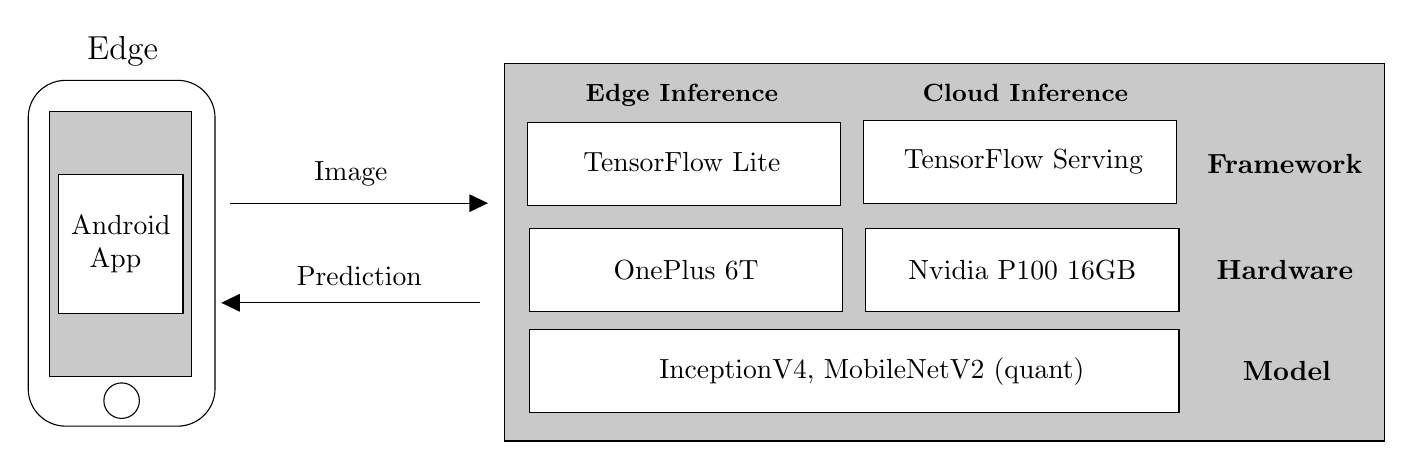
\begin{tikzpicture}[x=0.75pt,y=0.75pt,yscale=-1,xscale=1]
%uncomment if require: \path (0,485.57142639160156); %set diagram left start at 0, and has height of 485.57142639160156

%Straight Lines [id:da9993479608904674] 
\draw    (100.48,89) -- (223,89) ;
\draw [shift={(225,89)}, rotate = 540] [fill={rgb, 255:red, 0; green, 0; blue, 0 }  ][line width=0.75]  [draw opacity=0] (8.93,-4.29) -- (0,0) -- (8.93,4.29) -- cycle    ;

%Straight Lines [id:da5401559459790608] 
\draw    (98.48,137) -- (221,137) ;

\draw [shift={(96.48,137)}, rotate = 360] [fill={rgb, 255:red, 0; green, 0; blue, 0 }  ][line width=0.75]  [draw opacity=0] (8.93,-4.29) -- (0,0) -- (8.93,4.29) -- cycle    ;
%Shape: Rectangle [id:dp45054130026891115] 
\draw  [fill={rgb, 255:red, 201; green, 201; blue, 201 }  ,fill opacity=1 ] (233,21.57) -- (656.93,21.57) -- (656.93,203.57) -- (233,203.57) -- cycle ;
%Shape: Rectangle [id:dp21016153851852382] 
\draw  [fill={rgb, 255:red, 255; green, 255; blue, 255 }  ,fill opacity=1 ] (245,150) -- (557.93,150) -- (557.93,190) -- (245,190) -- cycle ;
%Shape: Rectangle [id:dp17739269402878732] 
\draw  [fill={rgb, 255:red, 255; green, 255; blue, 255 }  ,fill opacity=1 ] (244,50) -- (394.93,50) -- (394.93,90) -- (244,90) -- cycle ;
%Shape: Rectangle [id:dp9093436455970001] 
\draw  [fill={rgb, 255:red, 255; green, 255; blue, 255 }  ,fill opacity=1 ] (406,49) -- (556.93,49) -- (556.93,89) -- (406,89) -- cycle ;
%Shape: Rectangle [id:dp14120602080303146] 
\draw  [fill={rgb, 255:red, 255; green, 255; blue, 255 }  ,fill opacity=1 ] (245,101) -- (395.93,101) -- (395.93,141) -- (245,141) -- cycle ;
%Shape: Rectangle [id:dp45473714544487454] 
\draw  [fill={rgb, 255:red, 255; green, 255; blue, 255 }  ,fill opacity=1 ] (407,101) -- (557.93,101) -- (557.93,141) -- (407,141) -- cycle ;
%Shape: Rectangle [id:dp4153343207585154] 
\draw  [fill={rgb, 255:red, 201; green, 201; blue, 201 }  ,fill opacity=1 ] (13.91,44.69) -- (82.34,44.69) -- (82.34,172.63) -- (13.91,172.63) -- cycle ;
%Rounded Rect [id:dp09380596237315397] 
\draw   (3.5,47.82) .. controls (3.5,37.88) and (11.56,29.82) .. (21.5,29.82) -- (75.5,29.82) .. controls (85.44,29.82) and (93.5,37.88) .. (93.5,47.82) -- (93.5,178.43) .. controls (93.5,188.37) and (85.44,196.43) .. (75.5,196.43) -- (21.5,196.43) .. controls (11.56,196.43) and (3.5,188.37) .. (3.5,178.43) -- cycle ;
%Shape: Ellipse [id:dp8964060056788943] 
\draw   (39.95,184.16) .. controls (39.95,179.43) and (43.78,175.6) .. (48.5,175.6) .. controls (53.22,175.6) and (57.05,179.43) .. (57.05,184.16) .. controls (57.05,188.88) and (53.22,192.71) .. (48.5,192.71) .. controls (43.78,192.71) and (39.95,188.88) .. (39.95,184.16) -- cycle ;
%Shape: Rectangle [id:dp85708751067272] 
\draw  [fill={rgb, 255:red, 255; green, 255; blue, 255 }  ,fill opacity=1 ] (18.19,75.22) -- (78.07,75.22) -- (78.07,142.1) -- (18.19,142.1) -- cycle ;

% Text Node
\draw (159,75) node  [align=left] {Image};
% Text Node
\draw (163,124) node  [align=left] {Prediction};
% Text Node
\draw (49,16) node  [align=left] {{\large Edge}};
% Text Node
\draw (409.96,170) node  [align=left] {InceptionV4, MobileNetV2 (quant)};
% Text Node
\draw (318.46,37) node  [align=left] {{\small \textbf{Edge Inference}}};
% Text Node
\draw (483.96,36) node  [align=left] {{\small \textbf{Cloud Inference}}};
% Text Node
\draw (318.46,69) node  [align=left] {TensorFlow Lite};
% Text Node
\draw (482.96,68.79) node  [align=left] {TensorFlow Serving};
% Text Node
\draw (320.46,121) node  [align=left] {OnePlus 6T};
% Text Node
\draw (482.46,121) node  [align=left] {Nvidia P100 16GB};
% Text Node
\draw (608.96,70) node  [align=left] {\textbf{Framework}};
% Text Node
\draw (608.96,121) node  [align=left] {\textbf{Hardware}};
% Text Node
\draw (609.96,170) node  [align=left] {\textbf{Model}};
% Text Node
\draw (48.13,108.66) node  [align=left] {Android\\ \ \ App};


\end{tikzpicture}}
\caption{Experimental Design Architecture}
\label{fig:expDesign}
\end{figure}


\subsection{Hardware Devices}
\subsubsection{Edge}
\label{chap:hardwareEdge}
As the edge device we will use the OnePlus 6T (ONEPLUS A6013). This state of the art smartphone is powered by a Qualcomm Snapdragon 845 CPU(Octa-core, up to 2.8 GHz), Adreno 630 GPU, 8 GB of memory and runs on OxygenOS 9.0.11, which is based on Android 9.
%%Cite from AI bechmark paper
\subsubsection{Cloud}
%The Nvidia DGX-1 will serve as the cloud-backend for the experiments. This server consists of 8$\times$Tesla V100 providing 1000 TFLOPS as well as 256 GB GPU memory and 512 GB system memory.
We use a virtual server hosted at the LRZ, which has 32 cores (16 real cores with hyperthreading), 240 GB of memory, a Tesla P100 16 GB PCIe GPGPU and a 800 PCIe SSD.

The server runs on Ubuntu 16.04 CUDA 9.1 PGI 17.9 nvidia-docker 2.0.3+docker18.03.1-1.
\subsection{Deep Learning Inference Framework}
We use two open source machine learning frameworks, both based on TensorFlow, for the experiments, TensorFlow Lite and TensorFlow Serving. We decided to use these framework, because they are open source and support, at the point of this theses, most of the operations needed for the popular image classification models as well as an increasing number of hardware accelerators and operating systems for both edge and cloud inference.
TensorFlow provides official releases of deep learning models, that are well maintained and tested, including the ones we use in this thesis.

This section only gives a brief overview of the most important aspects of the frameworks, for detailed information consider the TensorFlow Lite\cite{tfLite}  and TensorFlow Serving\cite{tfServing} websites, on which this section is partly based on, or the corresponding GitHub repositories.
\subsubsection{TensorFlow Lite}
\label{chap:TFLite}
TensorFlow Lite (Release 1.12.0) was developed for mobile and embedded devices and is a lightweight solution of TensorFlow and thus will be used for the edge inference experiments.

%%Mention NNAPI support?
At the moment only model inference can be done by TensorFlow Lite, not model training.
It supports acceleration with GPU or other accelerators as well was portability to Android, iOS and other IoT devices.

\paragraph{Android NNAPI}
\label{chap:NNAPI}
TensorFlow Lite is also compatible with the Android Neural Networks API (NNAPI). This API
is designed to speed up computationally intensive machine learning operations and can be used by TensorFlow Lite to improve inference performance. During inference NNAPI "can
efficiently distribute the computation workload across available on-device processors, including dedicated neural network chips, GPUs and DSPs"\cite{DBLP:journals/corr/abs-1810-01109}.

Figure \ref{fig:NNAPIarchitecture} shows the architecture of the NNAPI. In our use case the application is our android benchmark application presented in section \ref{chap:androidApp} and the machine learning framework we use is TensorFlow Lite.
\begin{figure}[!htb]
\centering
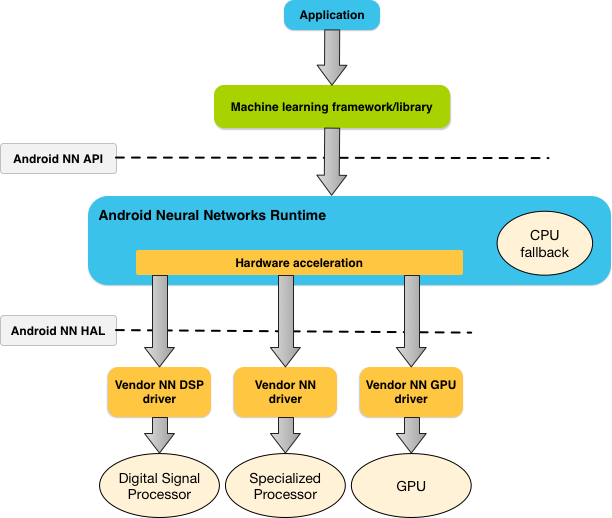
\includegraphics[width=0.5\textwidth]{./Bilder/nnapi_architecture.png}
\caption{System architecture for NNAPI framework \cite{NNAPI}}
\label{fig:NNAPIarchitecture}
\end{figure}


\paragraph{Hosting Models}
TensorFlow Lite expects models in their own \emph{FlatBuffer} file  format(\emph{.tflite}). Therefore models need to be converted to this format, before TensorFlow Lite can load them. This conversion can be done using the TensorFlow Lite Converter, which supports various formats of trained TensorFlow models.
After conversion a \emph{.tflite} model can be loaded by an object of the Interpreter class.
\paragraph{Run Prediction}

To then run the inference process in TensorFlow Lite the run method of Interpreter object with a loaded model needs to be called. To call this function two objects need to be passed, first the input for the given model and second the output object, where the prediction response from the inference operation get stored. 
\begin{figure}[H]
\centering



\tikzset{every picture/.style={line width=0.75pt}} %set default line width to 0.75pt        

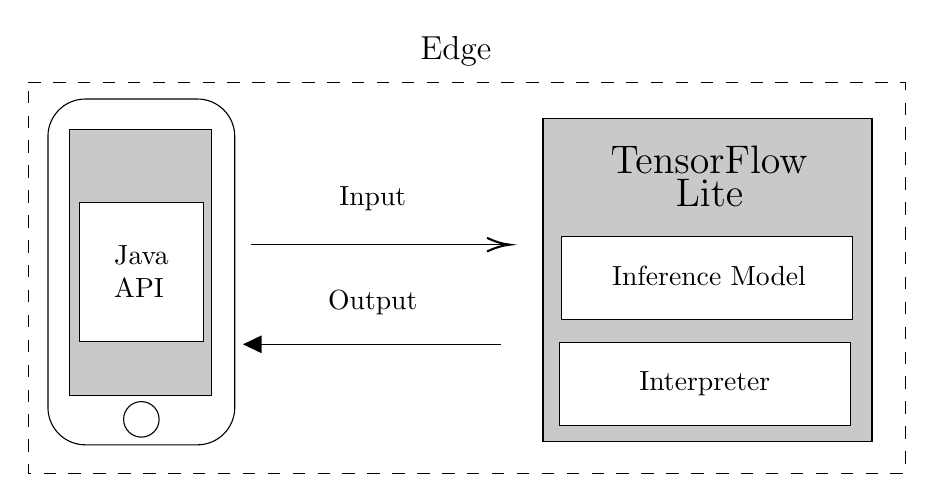
\begin{tikzpicture}[x=0.75pt,y=0.75pt,yscale=-1,xscale=1]
%uncomment if require: \path (0,300); %set diagram left start at 0, and has height of 300

%Shape: Rectangle [id:dp13292222689234756] 
\draw  [fill={rgb, 255:red, 201; green, 201; blue, 201 }  ,fill opacity=1 ] (61.91,111.69) -- (130.34,111.69) -- (130.34,239.63) -- (61.91,239.63) -- cycle ;
%Rounded Rect [id:dp7897713915001106] 
\draw   (51.5,114.82) .. controls (51.5,104.88) and (59.56,96.82) .. (69.5,96.82) -- (123.5,96.82) .. controls (133.44,96.82) and (141.5,104.88) .. (141.5,114.82) -- (141.5,245.43) .. controls (141.5,255.37) and (133.44,263.43) .. (123.5,263.43) -- (69.5,263.43) .. controls (59.56,263.43) and (51.5,255.37) .. (51.5,245.43) -- cycle ;
%Shape: Ellipse [id:dp9670901006981827] 
\draw   (87.95,251.16) .. controls (87.95,246.43) and (91.78,242.6) .. (96.5,242.6) .. controls (101.22,242.6) and (105.05,246.43) .. (105.05,251.16) .. controls (105.05,255.88) and (101.22,259.71) .. (96.5,259.71) .. controls (91.78,259.71) and (87.95,255.88) .. (87.95,251.16) -- cycle ;
%Straight Lines [id:da9993479608904674] 
\draw    (149.48,167) -- (272,167) ;
\draw [shift={(274,167)}, rotate = 540] [color={rgb, 255:red, 0; green, 0; blue, 0 }  ][line width=0.75]    (10.93,-3.29) .. controls (6.95,-1.4) and (3.31,-0.3) .. (0,0) .. controls (3.31,0.3) and (6.95,1.4) .. (10.93,3.29)   ;

%Straight Lines [id:da5401559459790608] 
\draw    (147.48,215) -- (270,215) ;

\draw [shift={(145.48,215)}, rotate = 360] [fill={rgb, 255:red, 0; green, 0; blue, 0 }  ][line width=0.75]  [draw opacity=0] (8.93,-4.29) -- (0,0) -- (8.93,4.29) -- cycle    ;
%Shape: Rectangle [id:dp45054130026891115] 
\draw  [fill={rgb, 255:red, 201; green, 201; blue, 201 }  ,fill opacity=1 ] (290,106) -- (448.5,106) -- (448.5,262) -- (290,262) -- cycle ;
%Shape: Rectangle [id:dp21016153851852382] 
\draw  [fill={rgb, 255:red, 255; green, 255; blue, 255 }  ,fill opacity=1 ] (299,163) -- (439,163) -- (439,203) -- (299,203) -- cycle ;
%Shape: Rectangle [id:dp8946256165796296] 
\draw  [fill={rgb, 255:red, 255; green, 255; blue, 255 }  ,fill opacity=1 ] (298,214) -- (438,214) -- (438,254) -- (298,254) -- cycle ;
%Shape: Rectangle [id:dp1345031923489386] 
\draw  [dash pattern={on 4.5pt off 4.5pt}] (42,89) -- (464.5,89) -- (464.5,277.4) -- (42,277.4) -- cycle ;
%Shape: Rectangle [id:dp7242946292477495] 
\draw  [fill={rgb, 255:red, 255; green, 255; blue, 255 }  ,fill opacity=1 ] (66.56,146.69) -- (126.44,146.69) -- (126.44,213.56) -- (66.56,213.56) -- cycle ;

% Text Node
\draw (208,145) node  [align=left] {Input};
% Text Node
\draw (248,74) node  [align=left] {{\large Edge}};
% Text Node
\draw (370,134) node  [align=left] {{\Large TensorFlow}\\{\Large  \ \ \ \ \ Lite}};
% Text Node
\draw (370,182) node  [align=left] {Inference Model};
% Text Node
\draw (208,195) node  [align=left] {Output};
% Text Node
\draw (368,234) node  [align=left] {Interpreter};
% Text Node
\draw (96.5,180.12) node  [align=left] {Java\\ API};


\end{tikzpicture}
\caption{Functionality of TensorFlow Lite}
\label{fig:edge}
\end{figure}
\subsubsection{TensorFlow Serving}
\label{chap:TFServing}
TensorFlow Serving (Release 1.12.0 VERIFY THIS AGAIN) will be used as the cloud inference framework, since it provides a framework to serve machine learning models in production environments. 



\paragraph{Hosting Models}
In order to host a model as a Servable in TensorFlow Serving, first a TensorFlow model needs to exported using TensorFlow's \emph{SavedModelBuilder}, resulting in a \emph{SavedModel protocol} buffer file along with the model’s variables and assets (Although TensorFlow Serving is optimized for TensorFlow models, the framework can be extended to serve other types of models).
%%Wieviel schreiben über signature, predict function etc?

Now the exported model can be loaded by a instance of Tensorflow Serving.
We use docker to start that instance, specifically nvidia-docker that allows us to run the inference operations on a GPU. For that TensorFlow Serving provides two docker images of their framework, one with CPU and the other with GPU support.

\paragraph{Run Prediction}
TensorFlow Serving supports two API for clients to create predictions requests: gRPC and REST. Since the gRPC protocol is supposed to deliver a better performance in the form of lower latencies and smaller payloads, we will use the gRPC API in this thesis.
Before a client can make a resquest to the server, a gRPC stub needs to be created in the first place, that allows us to call all methods implemented on the server. In our case we need to call TensorFlow Serving's \emph{Predict} method to start the inference process. The method needs to be passed a \emph{PredictRequest} object, which contains among other things the input data for the model, the shape of the input and the requested model.%model signature?

After the request is sent and handled the server response by sending back a \emph{PredictResponse} object. This object holds the predictions for the given input data in the form specified by the exported model.
This request and response process can also be seen in figure \ref{fig:cloud}

\begin{figure}[H]
\centering


\tikzset{every picture/.style={line width=0.75pt}} %set default line width to 0.75pt        

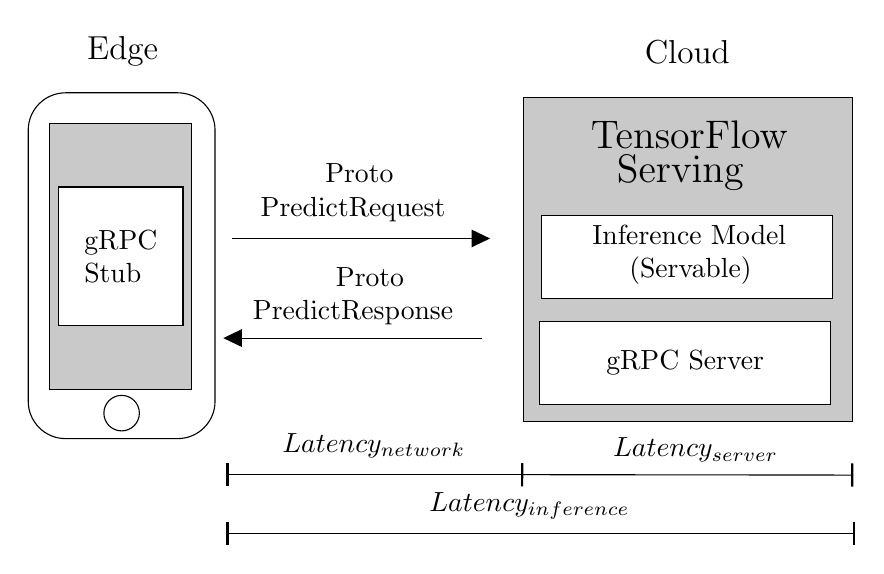
\begin{tikzpicture}[x=0.75pt,y=0.75pt,yscale=-1,xscale=1]
%uncomment if require: \path (0,300); %set diagram left start at 0, and has height of 300

%Straight Lines [id:da7072764839644827] 
\draw    (149.5,291) -- (451.5,291) ;
\draw [shift={(451.5,291)}, rotate = 180] [color={rgb, 255:red, 0; green, 0; blue, 0 }  ][line width=0.75]    (0,5.59) -- (0,-5.59)   ;
\draw [shift={(149.5,291)}, rotate = 180] [color={rgb, 255:red, 0; green, 0; blue, 0 }  ][line width=0.75]    (0,5.59) -- (0,-5.59)   ;
%Straight Lines [id:da9536138531960994] 
\draw    (291.5,262.8) -- (450.5,263) ;
\draw [shift={(450.5,263)}, rotate = 180.07] [color={rgb, 255:red, 0; green, 0; blue, 0 }  ][line width=0.75]    (0,5.59) -- (0,-5.59)   ;
\draw [shift={(291.5,262.8)}, rotate = 180.07] [color={rgb, 255:red, 0; green, 0; blue, 0 }  ][line width=0.75]    (0,5.59) -- (0,-5.59)   ;
%Shape: Rectangle [id:dp8902536871651789] 
\draw  [fill={rgb, 255:red, 201; green, 201; blue, 201 }  ,fill opacity=1 ] (63.91,93.69) -- (132.34,93.69) -- (132.34,221.63) -- (63.91,221.63) -- cycle ;
%Rounded Rect [id:dp41557214204551274] 
\draw   (53.5,96.82) .. controls (53.5,86.88) and (61.56,78.82) .. (71.5,78.82) -- (125.5,78.82) .. controls (135.44,78.82) and (143.5,86.88) .. (143.5,96.82) -- (143.5,227.43) .. controls (143.5,237.37) and (135.44,245.43) .. (125.5,245.43) -- (71.5,245.43) .. controls (61.56,245.43) and (53.5,237.37) .. (53.5,227.43) -- cycle ;
%Shape: Ellipse [id:dp8878397246816687] 
\draw   (89.95,233.16) .. controls (89.95,228.43) and (93.78,224.6) .. (98.5,224.6) .. controls (103.22,224.6) and (107.05,228.43) .. (107.05,233.16) .. controls (107.05,237.88) and (103.22,241.71) .. (98.5,241.71) .. controls (93.78,241.71) and (89.95,237.88) .. (89.95,233.16) -- cycle ;
%Straight Lines [id:da5813802620369573] 
\draw    (151.48,149) -- (274,149) ;
\draw [shift={(276,149)}, rotate = 540] [fill={rgb, 255:red, 0; green, 0; blue, 0 }  ][line width=0.75]  [draw opacity=0] (8.93,-4.29) -- (0,0) -- (8.93,4.29) -- cycle    ;

%Straight Lines [id:da16220168680973557] 
\draw    (149.48,197) -- (272,197) ;

\draw [shift={(147.48,197)}, rotate = 360] [fill={rgb, 255:red, 0; green, 0; blue, 0 }  ][line width=0.75]  [draw opacity=0] (8.93,-4.29) -- (0,0) -- (8.93,4.29) -- cycle    ;
%Shape: Rectangle [id:dp8411150472244695] 
\draw  [fill={rgb, 255:red, 201; green, 201; blue, 201 }  ,fill opacity=1 ] (292,81) -- (450.5,81) -- (450.5,237) -- (292,237) -- cycle ;
%Shape: Rectangle [id:dp13557861576626729] 
\draw  [fill={rgb, 255:red, 255; green, 255; blue, 255 }  ,fill opacity=1 ] (301,138) -- (441,138) -- (441,178) -- (301,178) -- cycle ;
%Shape: Rectangle [id:dp5681963435258506] 
\draw  [fill={rgb, 255:red, 255; green, 255; blue, 255 }  ,fill opacity=1 ] (68.19,124.22) -- (128.07,124.22) -- (128.07,191.1) -- (68.19,191.1) -- cycle ;
%Shape: Rectangle [id:dp7458124222136935] 
\draw  [fill={rgb, 255:red, 255; green, 255; blue, 255 }  ,fill opacity=1 ] (300,189) -- (440,189) -- (440,229) -- (300,229) -- cycle ;
%Straight Lines [id:da6846625455377753] 
\draw    (149.5,262.8) -- (291.5,262.8) ;
\draw [shift={(291.5,262.8)}, rotate = 180] [color={rgb, 255:red, 0; green, 0; blue, 0 }  ][line width=0.75]    (0,5.59) -- (0,-5.59)   ;
\draw [shift={(149.5,262.8)}, rotate = 180] [color={rgb, 255:red, 0; green, 0; blue, 0 }  ][line width=0.75]    (0,5.59) -- (0,-5.59)   ;

% Text Node
\draw (375,251) node  [align=left] {$\displaystyle Latency_{server}$$ $};
% Text Node
\draw (210,127) node  [align=left] { \ \ \ \ \ \ \ Proto\\PredictRequest};
% Text Node
\draw (99,59) node  [align=left] {{\large Edge}};
% Text Node
\draw (371,59) node  [align=left] {{\large Cloud}};
% Text Node
\draw (372,109) node  [align=left] {{\Large TensorFlow}\\{\Large  \ \ Serving}};
% Text Node
\draw (372,157) node  [align=left] {Inference Model\\ \ \ \ \ (Servable)};
% Text Node
\draw (210,177) node  [align=left] { \ \ \ \ \ \ \ \ \ Proto\\PredictResponse};
% Text Node
\draw (98.13,157.66) node  [align=left] {gRPC\\ Stub};
% Text Node
\draw (370,209) node  [align=left] {gRPC Server};
% Text Node
\draw (220,249) node  [align=left] {$\displaystyle Latency_{network}$$ $};
% Text Node
\draw (295,278) node  [align=left] {$\displaystyle Latency_{inference}$$ $};


\end{tikzpicture}
\caption{Basic Functionality of TensorFlow Serving}
\label{fig:cloud}
\end{figure}
\subsection{Models}
\label{chap:models}
We will benchmark two different image classification models in this thesis, MobileNetV2 and InceptionV4, the first is optimized for mobile deployment and the second towards high accuracy.
Both models are trained on a ImageNet dataset consisting of 1001 image classes (1000 image classes + 1 class for other image classes).
An overview of the models can be seen in table \ref{table:modelOverview} in the form of top-5 accuracy (a prediction is classified as accurate if the five labels with the highest confidence contain the real class of the input image), the input size of the model, the number of parameters in millions and the model size in the TensorFlow Lite format.
InceptionV4 has $4.5\%$ more accuracy than MobileNetV2, but also more than $12$ times more parameters and $7.5$ times larger TensorFlow Lite model size.
MobileNetV2 also uses a smaller input sizes of $224\times224$ than InceptionV4's $299\times299$ input size.
\begin{table}[H]
%CITE inception params ned vergessen
%http://dgschwend.github.io/netscope/#/preset/inceptionv4
\caption{Overview of used models}
\label{table:modelOverview}
\begin{tabular}{@{}lllll@{}}
\toprule
Model & Parameters & Top-5 Accuracy\cite{modelspecs} & Input Size & TF Lite Model Size \\
\midrule
InceptionV4 & $42.68$M & $95.1\%$ & $299\times299$ & $107.7$MB \\
MobileNetV2 1.0 & $3.47$M\cite{DBLP:journals/corr/abs-1801-04381} & $90.6\%$ & $224\times224$ & $14$MB \\
\begin{tabular}[c]{@{}l@{}}MobileNetV2 1.0\\quantized\end{tabular}  & $3.47$M\cite{DBLP:journals/corr/abs-1801-04381} & $89.9\%$ & $224\times224$ & $3.4$MB\\
\bottomrule
\end{tabular}
\end{table}
For the TensorFlow Lite version we use the models provided on the TensorFlow Lite website \cite{tfLiteModels}.
To convert model suitable for TensorFlow Serving, we use the TensorFlow-Slim library \cite{tfSlim}, where maintained and tested implementations of popular image classification models are being published. For both Serving and Lite we use the same training checkpoint to get the same weights for the graphs.

In the following we give a brief overview of the models, their unique building blocks and the intuition behind them.
For full details please refer to \cite{DBLP:journals/corr/abs-1801-04381} and \cite{InceptionV4}.

\subsubsection{MobileNetV2}
MobileNetV2 (version 1.0) is a successor of MobileNetV1 and is "specifically tailored for mobile and resource
constrained environments" \cite{DBLP:journals/corr/abs-1801-04381}. The authors do this by "significantly decreasing the number of operations and the memory needed while retaining the same accuracy"  \cite{DBLP:journals/corr/abs-1801-04381} and introducing a new layer module called "the
inverted residual with linear bottleneck".

This module is visualized in figure \ref{fig:bottleneckBlock} and consists of two parts: The inverted residual block and a shortcut from the input to the output.
In a first step of the inverted residual block the channel dimension of the input are expanded with the use of a pointwise $1\times1$ convolution layer. 
Afterwards depthwise $3\times3$ convolution is applied to the expanded input. Then again a pointwise $1\times1$ convolution gets used, but this time the dimensions are decreased instead of increased.

The intuition behind this module is that the expansion decodes information ensuring that the features can be extracted during the depthwise convolution. The extracted features then get encoded again by reducing the dimensions.
To improve the backpropagation of the gradient across multiple layers during the training the authors add the shortcut to the module, resulting in faster training and better accuracy.
The bottleneck module can be implemented very memory efficient, thus particularly fit for edge inference.

Figure \ref{fig:MobileNetArchi} displays the overall architecture of the model, with the majority of the building blocks being the bottleneck modules.
All bottleneck modules in a sequence have the same number of output channels and use a stride of $1$, except for the first bottleneck block in a sequence. All spatial convolutions use $3\times3$ kernels. 
Although not depicted on the figure, the model uses dropout and batch normalization during training.
%%expanstionf actor?
%%$$shortcut!! expanded by a "expansion factor" varying for different seqences

\begin{figure}[!htb]
\centering
   \resizebox{.7\linewidth}{!}{

\tikzset{every picture/.style={line width=0.75pt}} %set default line width to 0.75pt        

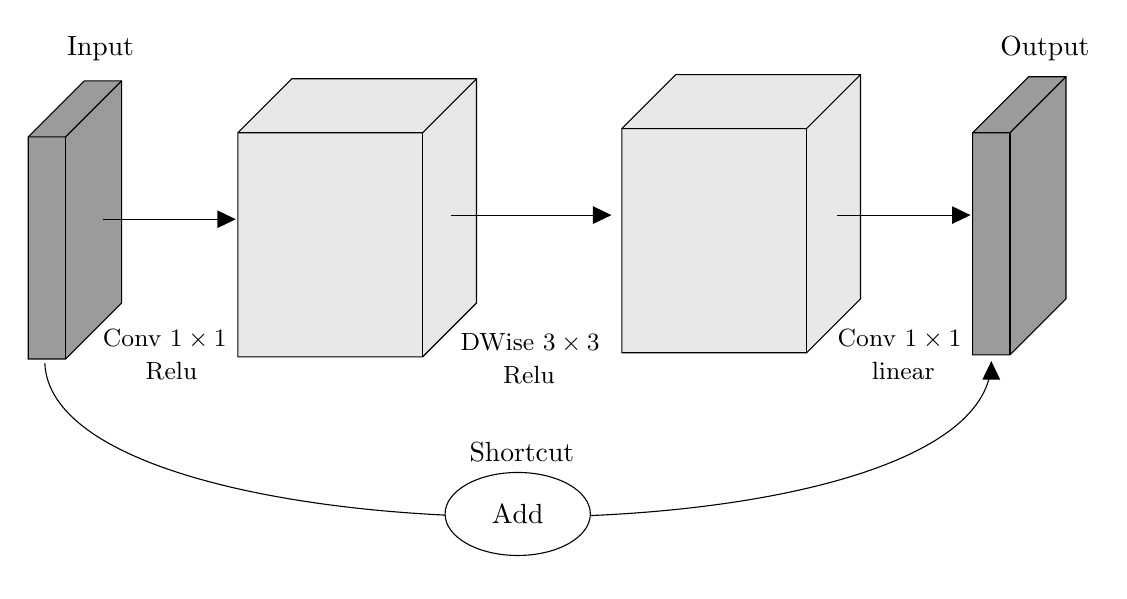
\begin{tikzpicture}[x=0.75pt,y=0.75pt,yscale=-1,xscale=1]
%uncomment if require: \path (0,600); %set diagram left start at 0, and has height of 600

%Shape: Cube [id:dp0950450187441989] 
\draw  [fill={rgb, 255:red, 155; green, 155; blue, 155 }  ,fill opacity=1 ] (24.17,60.33) -- (51.17,33.33) -- (69.17,33.33) -- (69.17,140.33) -- (42.17,167.33) -- (24.17,167.33) -- cycle ; \draw   (69.17,33.33) -- (42.17,60.33) -- (24.17,60.33) ; \draw   (42.17,60.33) -- (42.17,167.33) ;
%Shape: Cube [id:dp5388410753431343] 
\draw  [fill={rgb, 255:red, 155; green, 155; blue, 155 }  ,fill opacity=1 ] (479.17,58.33) -- (506.17,31.33) -- (524.17,31.33) -- (524.17,138.33) -- (497.17,165.33) -- (479.17,165.33) -- cycle ; \draw   (524.17,31.33) -- (497.17,58.33) -- (479.17,58.33) ; \draw   (497.17,58.33) -- (497.17,165.33) ;
%Shape: Cube [id:dp5352049268129733] 
\draw  [fill={rgb, 255:red, 232; green, 232; blue, 232 }  ,fill opacity=1 ] (125.17,58.33) -- (151.17,32.33) -- (240.17,32.33) -- (240.17,140.33) -- (214.17,166.33) -- (125.17,166.33) -- cycle ; \draw   (240.17,32.33) -- (214.17,58.33) -- (125.17,58.33) ; \draw   (214.17,58.33) -- (214.17,166.33) ;
%Shape: Cube [id:dp5972901431854747] 
\draw  [fill={rgb, 255:red, 232; green, 232; blue, 232 }  ,fill opacity=1 ] (310.17,56.33) -- (336.17,30.33) -- (425.17,30.33) -- (425.17,138.33) -- (399.17,164.33) -- (310.17,164.33) -- cycle ; \draw   (425.17,30.33) -- (399.17,56.33) -- (310.17,56.33) ; \draw   (399.17,56.33) -- (399.17,164.33) ;
%Curve Lines [id:da4213776555105224] 
\draw    (32.17,169.33) .. controls (36.15,266.84) and (483.66,269.31) .. (488.13,169.84) ;
\draw [shift={(488.17,168.33)}, rotate = 450] [fill={rgb, 255:red, 0; green, 0; blue, 0 }  ][line width=0.75]  [draw opacity=0] (8.93,-4.29) -- (0,0) -- (8.93,4.29) -- cycle    ;

%Straight Lines [id:da7525961556824932] 
\draw    (60,100) -- (122.17,100) ;
\draw [shift={(124.17,100)}, rotate = 180] [fill={rgb, 255:red, 0; green, 0; blue, 0 }  ][line width=0.75]  [draw opacity=0] (8.93,-4.29) -- (0,0) -- (8.93,4.29) -- cycle    ;

%Straight Lines [id:da7778926134720376] 
\draw    (228,98) -- (303.17,98) ;
\draw [shift={(305.17,98)}, rotate = 180] [fill={rgb, 255:red, 0; green, 0; blue, 0 }  ][line width=0.75]  [draw opacity=0] (8.93,-4.29) -- (0,0) -- (8.93,4.29) -- cycle    ;

%Straight Lines [id:da2814517292192529] 
\draw    (414,98) -- (476.17,98) ;
\draw [shift={(478.17,98)}, rotate = 180] [fill={rgb, 255:red, 0; green, 0; blue, 0 }  ][line width=0.75]  [draw opacity=0] (8.93,-4.29) -- (0,0) -- (8.93,4.29) -- cycle    ;

%Shape: Ellipse [id:dp8668947513316778] 
\draw  [fill={rgb, 255:red, 255; green, 255; blue, 255 }  ,fill opacity=1 ] (225,242) .. controls (225,230.95) and (240.67,222) .. (260,222) .. controls (279.33,222) and (295,230.95) .. (295,242) .. controls (295,253.05) and (279.33,262) .. (260,262) .. controls (240.67,262) and (225,253.05) .. (225,242) -- cycle ;

% Text Node
\draw (262,212) node  [align=left] {Shortcut};
% Text Node
\draw (90,165) node  [align=left] {{\small Conv $\displaystyle 1\times 1$}\\{\small  \ \ \ \ \ Relu}};
% Text Node
\draw (266,167) node  [align=left] {{\small DWise $\displaystyle 3\times 3$}\\{\small  \ \ \ \ \ Relu}};
% Text Node
\draw (444,165) node  [align=left] {{\small Conv $\displaystyle 1\times 1$}\\{\small  \ \ \ \ linear}};
% Text Node
\draw (260,242) node  [align=left] {Add};
% Text Node
\draw (59,18) node  [align=left] {Input};
% Text Node
\draw (514,18) node  [align=left] {Output};


\end{tikzpicture}}
\caption{Inverted Residual Block (bottleneck)}
\label{fig:bottleneckBlock}
%%NO DROPOUT AT INFERENCE
\end{figure}


\begin{comment}


\begin{table}[]

\centering
\caption{MobilenetV2 architecture \cite{DBLP:journals/corr/abs-1801-04381}}
\label{table:mobilenetArchi}
\begin{tabular}{@{}llllll@{}}

\toprule
Input & Operator & t & c & n & s \\ \midrule
$224^2\times 3$ & conv2d & - & 32 & 1 & 2 \\
$112^2\times 32$ & bottleneck & 1 & 16 & 1 & 1 \\
$112^2\times 16$ & bottleneck & 6 & 24 & 2 & 2 \\
$56^2\times 24$ & bottleneck & 6 & 32 & 3 & 2 \\
$28^2\times 23$ & bottleneck & 6 & 64 & 4 & 2 \\
$14^2\times 64$ & bottleneck & 6 & 96 & 3 & 1 \\
$14^2\times 96$ & bottleneck & 6 & 160 & 3 & 2 \\
$7^2\times 160$ & bottleneck & 6 & 320 & 1 & 1 \\
$7^2\times 320$ & conv2d 1x1 & - & 1280 & 1 & 1 \\
$7^2\times 1280$ & avgpool 7x7 & - & - & 1 & - \\
$1\times 1\times 1280$ & conv2d 1x1 & - & k & - &  \\ \bottomrule
\end{tabular}
\end{table}
\end{comment}
\paragraph{Quantization}
Quantization of MobileNetV2, using the techniques presented in section \ref{chap:quant}, results in a  0.7\% loss of top-5 accuracy, but therefore has lost 75\% of its model size (see table \ref{table:modelOverview}) and is supposed to deliver a better inference performance, which we will evaluate in the experiments.



\subsubsection{Inception V4}
%%Add infos about stem and reduction
InceptionV4, published in \cite{InceptionV4}, is a large image classification network with high accuracy, but also with a high number of parameters leading to higher computational demands than MobileNetV2 and thus larger impact on inference performance.
In comparison to its previous versions InceptionV4 is built with "a more uniform simplified architecture and more inception modules". 

The general architecture of the network can be seen in figure \ref{fig:inceptionv4Archi} with the fundamental building blocks being multiple Inception (A-C) and Reduction(A-B) modules. 
An example for both of these modules can be seen in figures \ref{fig:InceptionA} and \ref{fig:InceptionReduction}.
Inception modules are built of multiple convolutions with multiple filters and pooling layers in parallel within the same layer.
After the convolutions the output of all convolutions are concatenated.
The intuition behind this parallelism is to give the model multiple convolution choices for a given input and let the model learn itself the best feature extractor. An additional benefit is that the model can extract both local and more complex feature from an input.

To reduce the dimensionality before computational expensive large convolutions, and thus speed up training, the authors introduce the Reduction block containing small $1\times1$ convolutions.   %genauer erklären




\begin{figure}[!htb]
\centering
\begin{subfigure}[b]{.95\textwidth}
\centering
   \resizebox{.8\linewidth}{!}{

\tikzset{every picture/.style={line width=0.75pt}} %set default line width to 0.75pt        

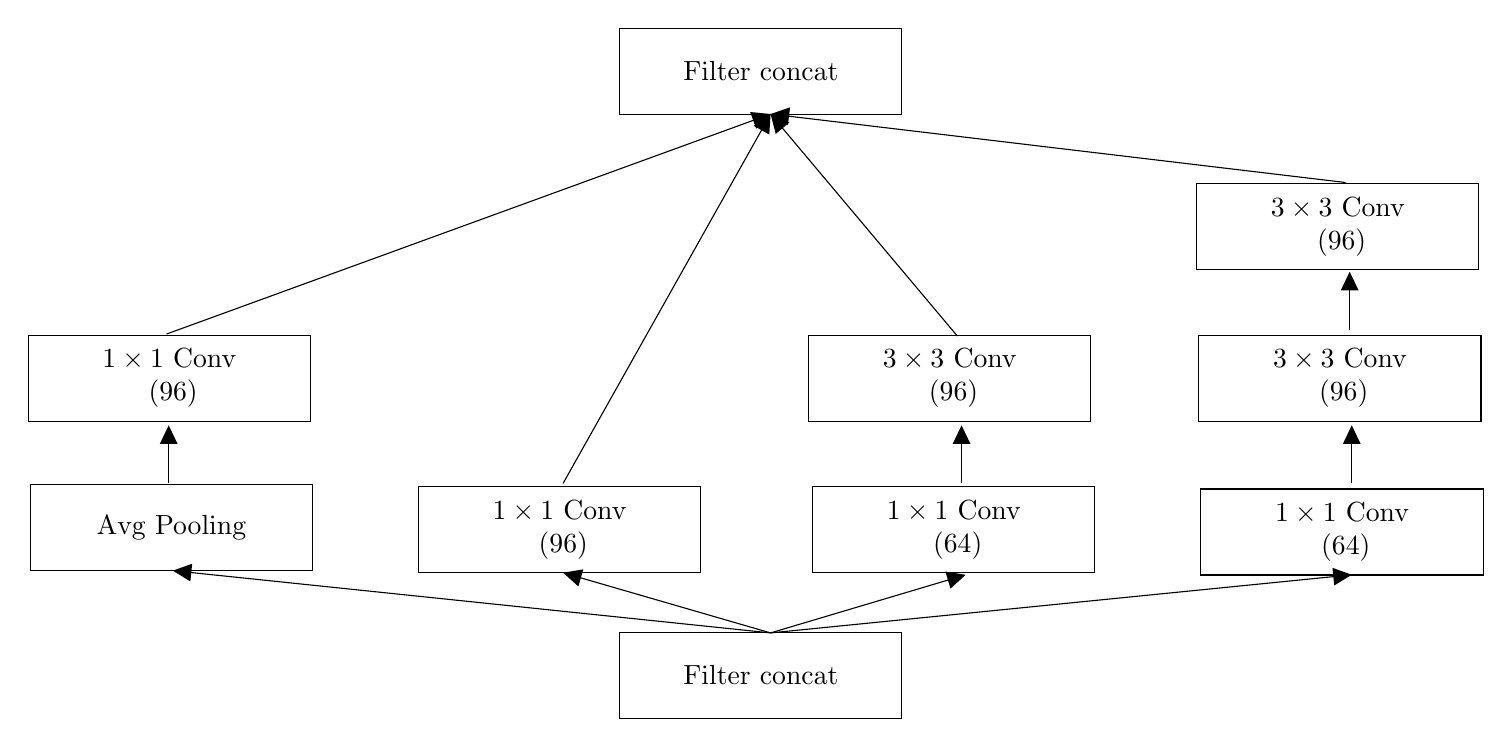
\begin{tikzpicture}[x=0.75pt,y=0.75pt,yscale=-1,xscale=1]
%uncomment if require: \path (0,550.3333358764648); %set diagram left start at 0, and has height of 550.3333358764648

%Flowchart: Process [id:dp8446713243434529] 
\draw   (508,479) -- (643.93,479) -- (643.93,520.43) -- (508,520.43) -- cycle ;
%Flowchart: Process [id:dp8389212433494444] 
\draw   (224,408) -- (359.93,408) -- (359.93,449.43) -- (224,449.43) -- cycle ;
%Flowchart: Process [id:dp9696039225192121] 
\draw   (411,409) -- (546.93,409) -- (546.93,450.43) -- (411,450.43) -- cycle ;
%Flowchart: Process [id:dp31126408548780393] 
\draw   (601,409) -- (736.93,409) -- (736.93,450.43) -- (601,450.43) -- cycle ;
%Flowchart: Process [id:dp739948518816423] 
\draw   (788,410) -- (923.93,410) -- (923.93,451.43) -- (788,451.43) -- cycle ;
%Straight Lines [id:da20227844614554824] 
\draw    (580.67,479.33) -- (294.66,449.54) ;
\draw [shift={(292.67,449.33)}, rotate = 365.95] [fill={rgb, 255:red, 0; green, 0; blue, 0 }  ][line width=0.75]  [draw opacity=0] (8.93,-4.29) -- (0,0) -- (8.93,4.29) -- cycle    ;

%Straight Lines [id:da9079516459586603] 
\draw    (580.67,479.33) -- (482.59,450.89) ;
\draw [shift={(480.67,450.33)}, rotate = 376.16999999999996] [fill={rgb, 255:red, 0; green, 0; blue, 0 }  ][line width=0.75]  [draw opacity=0] (8.93,-4.29) -- (0,0) -- (8.93,4.29) -- cycle    ;

%Straight Lines [id:da7697048902828942] 
\draw    (580.67,479.33) -- (672.75,451.9) ;
\draw [shift={(674.67,451.33)}, rotate = 523.4100000000001] [fill={rgb, 255:red, 0; green, 0; blue, 0 }  ][line width=0.75]  [draw opacity=0] (8.93,-4.29) -- (0,0) -- (8.93,4.29) -- cycle    ;

%Straight Lines [id:da004295071242706339] 
\draw    (580.67,479.33) -- (858.68,451.53) ;
\draw [shift={(860.67,451.33)}, rotate = 534.29] [fill={rgb, 255:red, 0; green, 0; blue, 0 }  ][line width=0.75]  [draw opacity=0] (8.93,-4.29) -- (0,0) -- (8.93,4.29) -- cycle    ;

%Flowchart: Process [id:dp6126721254059377] 
\draw   (223,336) -- (358.93,336) -- (358.93,377.43) -- (223,377.43) -- cycle ;
%Flowchart: Process [id:dp6415327260036892] 
\draw   (599,336) -- (734.93,336) -- (734.93,377.43) -- (599,377.43) -- cycle ;
%Flowchart: Process [id:dp557242506777897] 
\draw   (787,336) -- (922.93,336) -- (922.93,377.43) -- (787,377.43) -- cycle ;
%Flowchart: Process [id:dp895045490145193] 
\draw   (786,263) -- (921.93,263) -- (921.93,304.43) -- (786,304.43) -- cycle ;
%Straight Lines [id:da042686267300120706] 
\draw    (290.67,407.33) -- (290.67,381.33) ;
\draw [shift={(290.67,379.33)}, rotate = 450] [fill={rgb, 255:red, 0; green, 0; blue, 0 }  ][line width=0.75]  [draw opacity=0] (8.93,-4.29) -- (0,0) -- (8.93,4.29) -- cycle    ;

%Straight Lines [id:da1451751743173857] 
\draw    (672.67,407.33) -- (672.67,381.33) ;
\draw [shift={(672.67,379.33)}, rotate = 450] [fill={rgb, 255:red, 0; green, 0; blue, 0 }  ][line width=0.75]  [draw opacity=0] (8.93,-4.29) -- (0,0) -- (8.93,4.29) -- cycle    ;

%Straight Lines [id:da7065201039263691] 
\draw    (860.67,407.33) -- (860.67,381.33) ;
\draw [shift={(860.67,379.33)}, rotate = 450] [fill={rgb, 255:red, 0; green, 0; blue, 0 }  ][line width=0.75]  [draw opacity=0] (8.93,-4.29) -- (0,0) -- (8.93,4.29) -- cycle    ;

%Straight Lines [id:da3529249322466719] 
\draw    (859.67,333.33) -- (859.67,307.33) ;
\draw [shift={(859.67,305.33)}, rotate = 450] [fill={rgb, 255:red, 0; green, 0; blue, 0 }  ][line width=0.75]  [draw opacity=0] (8.93,-4.29) -- (0,0) -- (8.93,4.29) -- cycle    ;

%Flowchart: Process [id:dp023795399666625805] 
\draw   (508,188) -- (643.93,188) -- (643.93,229.43) -- (508,229.43) -- cycle ;
%Straight Lines [id:da14696140485542641] 
\draw    (289.67,335.33) -- (578.79,230.02) ;
\draw [shift={(580.67,229.33)}, rotate = 519.99] [fill={rgb, 255:red, 0; green, 0; blue, 0 }  ][line width=0.75]  [draw opacity=0] (8.93,-4.29) -- (0,0) -- (8.93,4.29) -- cycle    ;

%Straight Lines [id:da7335126004687851] 
\draw    (480.67,407.33) -- (579.69,231.08) ;
\draw [shift={(580.67,229.33)}, rotate = 479.33] [fill={rgb, 255:red, 0; green, 0; blue, 0 }  ][line width=0.75]  [draw opacity=0] (8.93,-4.29) -- (0,0) -- (8.93,4.29) -- cycle    ;

%Straight Lines [id:da6191146997492387] 
\draw    (670.67,336.33) -- (581.95,230.86) ;
\draw [shift={(580.67,229.33)}, rotate = 409.93] [fill={rgb, 255:red, 0; green, 0; blue, 0 }  ][line width=0.75]  [draw opacity=0] (8.93,-4.29) -- (0,0) -- (8.93,4.29) -- cycle    ;

%Straight Lines [id:da444168686885831] 
\draw    (857.67,262.33) -- (582.65,229.57) ;
\draw [shift={(580.67,229.33)}, rotate = 366.78999999999996] [fill={rgb, 255:red, 0; green, 0; blue, 0 }  ][line width=0.75]  [draw opacity=0] (8.93,-4.29) -- (0,0) -- (8.93,4.29) -- cycle    ;


% Text Node
\draw (575.96,499.71) node  [align=left] {Filter concat};
% Text Node
\draw (291.96,428.71) node  [align=left] {Avg Pooling};
% Text Node
\draw (478.96,429.71) node  [align=left] {$\displaystyle 1\times 1$ Conv\\ \ \ \ \ \ (96)};
% Text Node
\draw (668.96,429.71) node  [align=left] {$\displaystyle 1\times 1$ Conv\\ \ \ \ \ \ (64)};
% Text Node
\draw (855.96,430.71) node  [align=left] {$\displaystyle 1\times 1$ Conv\\ \ \ \ \ \ (64)};
% Text Node
\draw (290.96,356.71) node  [align=left] {$\displaystyle 1\times 1$ Conv\\ \ \ \ \ \ (96)};
% Text Node
\draw (666.96,356.71) node  [align=left] {$\displaystyle 3\times 3$ Conv\\ \ \ \ \ \ (96)};
% Text Node
\draw (854.96,356.71) node  [align=left] {$\displaystyle 3\times 3$ Conv\\ \ \ \ \ \ (96)};
% Text Node
\draw (853.96,283.71) node  [align=left] {$\displaystyle 3\times 3$ Conv\\ \ \ \ \ \ (96)};
% Text Node
\draw (575.96,208.71) node  [align=left] {Filter concat};


\end{tikzpicture}}
   \caption{Inception-A module}
   \label{fig:InceptionA} 
\end{subfigure}

\vspace{1em}
\begin{subfigure}[b]{.95\textwidth}
\centering
   %%Verify the architectures again
   \resizebox{.6\linewidth}{!}{

\tikzset{every picture/.style={line width=0.75pt}} %set default line width to 0.75pt        

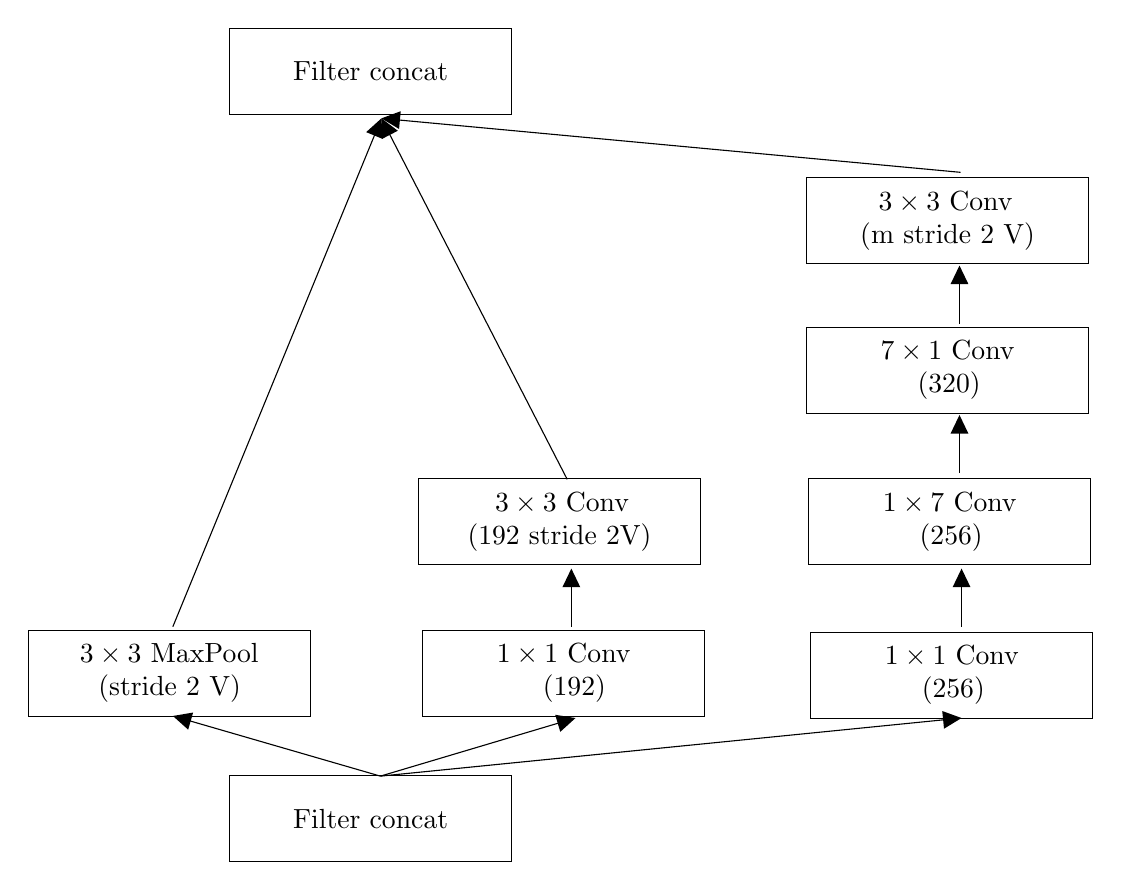
\begin{tikzpicture}[x=0.75pt,y=0.75pt,yscale=-1,xscale=1]
%uncomment if require: \path (0,470.3333282470703); %set diagram left start at 0, and has height of 470.3333282470703

%Flowchart: Process [id:dp24078826379297702] 
\draw   (528,418.9) -- (663.93,418.9) -- (663.93,460.33) -- (528,460.33) -- cycle ;
%Flowchart: Process [id:dp22165017848855517] 
\draw   (431,348.9) -- (566.93,348.9) -- (566.93,390.33) -- (431,390.33) -- cycle ;
%Flowchart: Process [id:dp6597264859137688] 
\draw   (621,348.9) -- (756.93,348.9) -- (756.93,390.33) -- (621,390.33) -- cycle ;
%Flowchart: Process [id:dp3799233367302206] 
\draw   (808,349.9) -- (943.93,349.9) -- (943.93,391.33) -- (808,391.33) -- cycle ;
%Straight Lines [id:da4490839848046586] 
\draw    (600.67,419.24) -- (502.59,390.8) ;
\draw [shift={(500.67,390.24)}, rotate = 376.16999999999996] [fill={rgb, 255:red, 0; green, 0; blue, 0 }  ][line width=0.75]  [draw opacity=0] (8.93,-4.29) -- (0,0) -- (8.93,4.29) -- cycle    ;

%Straight Lines [id:da38737183977033096] 
\draw    (600.67,419.24) -- (692.75,391.81) ;
\draw [shift={(694.67,391.24)}, rotate = 523.4100000000001] [fill={rgb, 255:red, 0; green, 0; blue, 0 }  ][line width=0.75]  [draw opacity=0] (8.93,-4.29) -- (0,0) -- (8.93,4.29) -- cycle    ;

%Straight Lines [id:da40057235552744497] 
\draw    (600.67,419.24) -- (878.68,391.44) ;
\draw [shift={(880.67,391.24)}, rotate = 534.29] [fill={rgb, 255:red, 0; green, 0; blue, 0 }  ][line width=0.75]  [draw opacity=0] (8.93,-4.29) -- (0,0) -- (8.93,4.29) -- cycle    ;

%Flowchart: Process [id:dp42511218119703864] 
\draw   (619,275.9) -- (754.93,275.9) -- (754.93,317.33) -- (619,317.33) -- cycle ;
%Flowchart: Process [id:dp6580432352234802] 
\draw   (807,275.9) -- (942.93,275.9) -- (942.93,317.33) -- (807,317.33) -- cycle ;
%Flowchart: Process [id:dp8669834254894924] 
\draw   (806,202.9) -- (941.93,202.9) -- (941.93,244.33) -- (806,244.33) -- cycle ;
%Straight Lines [id:da7396787751036953] 
\draw    (692.67,347.24) -- (692.67,321.24) ;
\draw [shift={(692.67,319.24)}, rotate = 450] [fill={rgb, 255:red, 0; green, 0; blue, 0 }  ][line width=0.75]  [draw opacity=0] (8.93,-4.29) -- (0,0) -- (8.93,4.29) -- cycle    ;

%Straight Lines [id:da2216611723462627] 
\draw    (880.67,347.24) -- (880.67,321.24) ;
\draw [shift={(880.67,319.24)}, rotate = 450] [fill={rgb, 255:red, 0; green, 0; blue, 0 }  ][line width=0.75]  [draw opacity=0] (8.93,-4.29) -- (0,0) -- (8.93,4.29) -- cycle    ;

%Straight Lines [id:da7609415385669374] 
\draw    (879.67,273.24) -- (879.67,247.24) ;
\draw [shift={(879.67,245.24)}, rotate = 450] [fill={rgb, 255:red, 0; green, 0; blue, 0 }  ][line width=0.75]  [draw opacity=0] (8.93,-4.29) -- (0,0) -- (8.93,4.29) -- cycle    ;

%Flowchart: Process [id:dp1491076780226832] 
\draw   (528,58.9) -- (663.93,58.9) -- (663.93,100.33) -- (528,100.33) -- cycle ;
%Straight Lines [id:da30781560796019103] 
\draw    (500.67,347.24) -- (600.41,104.18) ;
\draw [shift={(601.17,102.33)}, rotate = 472.31] [fill={rgb, 255:red, 0; green, 0; blue, 0 }  ][line width=0.75]  [draw opacity=0] (8.93,-4.29) -- (0,0) -- (8.93,4.29) -- cycle    ;

%Straight Lines [id:da24908463720618457] 
\draw    (690.67,276.24) -- (602.08,104.11) ;
\draw [shift={(601.17,102.33)}, rotate = 422.77] [fill={rgb, 255:red, 0; green, 0; blue, 0 }  ][line width=0.75]  [draw opacity=0] (8.93,-4.29) -- (0,0) -- (8.93,4.29) -- cycle    ;

%Flowchart: Process [id:dp01199680277761872] 
\draw   (806,130.9) -- (941.93,130.9) -- (941.93,172.33) -- (806,172.33) -- cycle ;
%Straight Lines [id:da3952124421996095] 
\draw    (879.67,201.24) -- (879.67,175.24) ;
\draw [shift={(879.67,173.24)}, rotate = 450] [fill={rgb, 255:red, 0; green, 0; blue, 0 }  ][line width=0.75]  [draw opacity=0] (8.93,-4.29) -- (0,0) -- (8.93,4.29) -- cycle    ;

%Straight Lines [id:da25220885973901197] 
\draw    (880.17,128.33) -- (603.16,102.52) ;
\draw [shift={(601.17,102.33)}, rotate = 365.32] [fill={rgb, 255:red, 0; green, 0; blue, 0 }  ][line width=0.75]  [draw opacity=0] (8.93,-4.29) -- (0,0) -- (8.93,4.29) -- cycle    ;


% Text Node
\draw (595.96,439.62) node  [align=left] {Filter concat};
% Text Node
\draw (498.96,369.62) node  [align=left] {$\displaystyle 3\times 3$ MaxPool\\ \ \ (stride $\displaystyle 2$ V)};
% Text Node
\draw (688.96,369.62) node  [align=left] {$\displaystyle 1\times 1$ Conv\\ \ \ \ \ \ ($\displaystyle 192$)};
% Text Node
\draw (875.96,370.62) node  [align=left] {$\displaystyle 1\times 1$ Conv\\ \ \ \ \ ($\displaystyle 256$)};
% Text Node
\draw (686.96,296.62) node  [align=left] {$\displaystyle \ \ \ 3\times 3$ Conv\\($\displaystyle 192$ stride $\displaystyle 2$V)};
% Text Node
\draw (874.96,296.62) node  [align=left] {$\displaystyle 1\times 7$ Conv\\ \ \ \ \ ($\displaystyle 256$)};
% Text Node
\draw (873.96,223.62) node  [align=left] {$\displaystyle 7\times 1$ Conv\\ \ \ \ \ ($\displaystyle 320$)};
% Text Node
\draw (595.96,79.62) node  [align=left] {Filter concat};
% Text Node
\draw (873.96,151.62) node  [align=left] {$\displaystyle \ \ 3\times 3$ Conv\\(m stride $\displaystyle 2$ V)};


\end{tikzpicture}}
   \caption{Reduction module (convolutions with "V" are valid, rest is same padded )}
   \label{fig:InceptionReduction}
\end{subfigure}

\caption{Special modules used by InceptionV4}

\end{figure}




Besides dropout InceptionV4 also benefits from the use of batch normalization during training.
%\begin{figure}[]
%\centering
%\resizebox{.45\linewidth}{!}{

\tikzset{every picture/.style={line width=0.75pt}} %set default line width to 0.75pt        

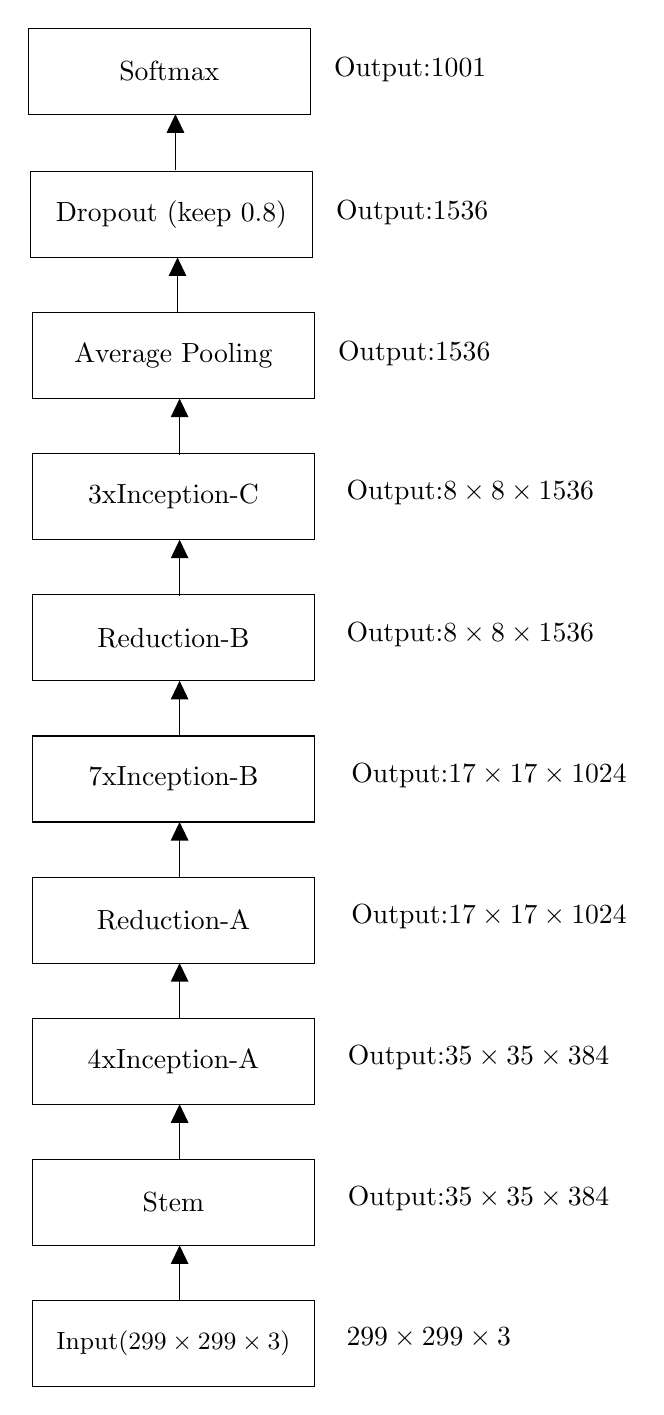
\begin{tikzpicture}[x=0.75pt,y=0.75pt,yscale=-1,xscale=1]
%uncomment if require: \path (0,742.7142868041992); %set diagram left start at 0, and has height of 742.7142868041992

%Flowchart: Process [id:dp9253173394290999] 
\draw   (98,621) -- (233.93,621) -- (233.93,662.43) -- (98,662.43) -- cycle ;
%Flowchart: Process [id:dp47578347996398307] 
\draw   (98,553) -- (233.93,553) -- (233.93,594.43) -- (98,594.43) -- cycle ;
%Straight Lines [id:da2925025767777827] 
\draw    (168.93,621.43) -- (168.93,596.43) ;
\draw [shift={(168.93,594.43)}, rotate = 450] [fill={rgb, 255:red, 0; green, 0; blue, 0 }  ][line width=0.75]  [draw opacity=0] (8.93,-4.29) -- (0,0) -- (8.93,4.29) -- cycle    ;

%Flowchart: Process [id:dp5382364848384393] 
\draw   (98,485) -- (233.93,485) -- (233.93,526.43) -- (98,526.43) -- cycle ;
%Straight Lines [id:da06940381159807729] 
\draw    (168.93,553.43) -- (168.93,528.43) ;
\draw [shift={(168.93,526.43)}, rotate = 450] [fill={rgb, 255:red, 0; green, 0; blue, 0 }  ][line width=0.75]  [draw opacity=0] (8.93,-4.29) -- (0,0) -- (8.93,4.29) -- cycle    ;

%Flowchart: Process [id:dp21301144435418706] 
\draw   (98,417) -- (233.93,417) -- (233.93,458.43) -- (98,458.43) -- cycle ;
%Straight Lines [id:da45627711718103714] 
\draw    (168.93,485.43) -- (168.93,460.43) ;
\draw [shift={(168.93,458.43)}, rotate = 450] [fill={rgb, 255:red, 0; green, 0; blue, 0 }  ][line width=0.75]  [draw opacity=0] (8.93,-4.29) -- (0,0) -- (8.93,4.29) -- cycle    ;

%Flowchart: Process [id:dp7231968775803179] 
\draw   (98,349) -- (233.93,349) -- (233.93,390.43) -- (98,390.43) -- cycle ;
%Straight Lines [id:da7165121439179447] 
\draw    (168.93,417.43) -- (168.93,392.43) ;
\draw [shift={(168.93,390.43)}, rotate = 450] [fill={rgb, 255:red, 0; green, 0; blue, 0 }  ][line width=0.75]  [draw opacity=0] (8.93,-4.29) -- (0,0) -- (8.93,4.29) -- cycle    ;

%Flowchart: Process [id:dp20620702942862734] 
\draw   (98,281) -- (233.93,281) -- (233.93,322.43) -- (98,322.43) -- cycle ;
%Straight Lines [id:da10564528480224444] 
\draw    (168.93,349.43) -- (168.93,324.43) ;
\draw [shift={(168.93,322.43)}, rotate = 450] [fill={rgb, 255:red, 0; green, 0; blue, 0 }  ][line width=0.75]  [draw opacity=0] (8.93,-4.29) -- (0,0) -- (8.93,4.29) -- cycle    ;

%Flowchart: Process [id:dp6409642010028676] 
\draw   (98,213) -- (233.93,213) -- (233.93,254.43) -- (98,254.43) -- cycle ;
%Straight Lines [id:da583110185704452] 
\draw    (168.93,281.43) -- (168.93,256.43) ;
\draw [shift={(168.93,254.43)}, rotate = 450] [fill={rgb, 255:red, 0; green, 0; blue, 0 }  ][line width=0.75]  [draw opacity=0] (8.93,-4.29) -- (0,0) -- (8.93,4.29) -- cycle    ;

%Flowchart: Process [id:dp747253235525678] 
\draw   (98,145) -- (233.93,145) -- (233.93,186.43) -- (98,186.43) -- cycle ;
%Straight Lines [id:da9482962038382927] 
\draw    (168.93,213.43) -- (168.93,188.43) ;
\draw [shift={(168.93,186.43)}, rotate = 450] [fill={rgb, 255:red, 0; green, 0; blue, 0 }  ][line width=0.75]  [draw opacity=0] (8.93,-4.29) -- (0,0) -- (8.93,4.29) -- cycle    ;

%Flowchart: Process [id:dp47103409298757426] 
\draw   (97,77) -- (232.93,77) -- (232.93,118.43) -- (97,118.43) -- cycle ;
%Straight Lines [id:da30249651940608824] 
\draw    (167.93,145.43) -- (167.93,120.43) ;
\draw [shift={(167.93,118.43)}, rotate = 450] [fill={rgb, 255:red, 0; green, 0; blue, 0 }  ][line width=0.75]  [draw opacity=0] (8.93,-4.29) -- (0,0) -- (8.93,4.29) -- cycle    ;

%Flowchart: Process [id:dp5661311837160838] 
\draw   (96,8) -- (231.93,8) -- (231.93,49.43) -- (96,49.43) -- cycle ;
%Straight Lines [id:da5142446239913938] 
\draw    (166.93,76.43) -- (166.93,51.43) ;
\draw [shift={(166.93,49.43)}, rotate = 450] [fill={rgb, 255:red, 0; green, 0; blue, 0 }  ][line width=0.75]  [draw opacity=0] (8.93,-4.29) -- (0,0) -- (8.93,4.29) -- cycle    ;


% Text Node
\draw (165.96,641.71) node  [align=left] {{\small Input($\displaystyle 299\times 299\times 3$)}};
% Text Node
\draw (165.96,573.71) node  [align=left] {Stem};
% Text Node
\draw (289,639) node  [align=left] {$\displaystyle 299\times 299\times 3$};
% Text Node
\draw (313,572) node  [align=left] {Output:$\displaystyle 35\times 35\times 384$};
% Text Node
\draw (165.96,505.71) node  [align=left] {4xInception-A};
% Text Node
\draw (313,504) node  [align=left] {Output:$\displaystyle 35\times 35\times 384$};
% Text Node
\draw (165.96,437.71) node  [align=left] {Reduction-A};
% Text Node
\draw (318,436) node  [align=left] {Output:$\displaystyle 17\times 17\times 1024$};
% Text Node
\draw (165.96,369.71) node  [align=left] {7xInception-B};
% Text Node
\draw (318,368) node  [align=left] {Output:$\displaystyle 17\times 17\times 1024$};
% Text Node
\draw (165.96,301.71) node  [align=left] {Reduction-B};
% Text Node
\draw (309,300) node  [align=left] {Output:$\displaystyle 8\times 8\times 1536$};
% Text Node
\draw (165.96,233.71) node  [align=left] {3xInception-C};
% Text Node
\draw (309,232) node  [align=left] {Output:$\displaystyle 8\times 8\times 1536$};
% Text Node
\draw (165.96,165.71) node  [align=left] {Average Pooling};
% Text Node
\draw (282,165) node  [align=left] {Output:$\displaystyle 1536$};
% Text Node
\draw (164.96,97.71) node  [align=left] {Dropout (keep $\displaystyle 0.8$)};
% Text Node
\draw (281,97) node  [align=left] {Output:$\displaystyle 1536$};
% Text Node
\draw (163.96,28.71) node  [align=left] {Softmax};
% Text Node
\draw (280,28) node  [align=left] {Output:$\displaystyle 1001$};


\end{tikzpicture}}
%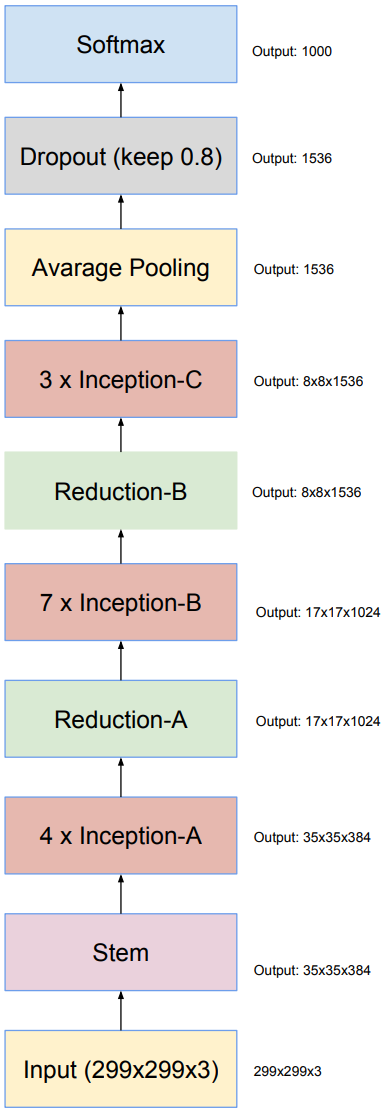
\includegraphics[angle=90,width=0.94\textwidth]{./Bilder/inceptionV4_architecture.png}
%\caption{InceptionV4 architecture \cite{InceptionV4}}
%\label{fig:inceptionv4}
%\end{figure}

\begin{figure}[!htb]
\centering
\begin{subfigure}[t]{0.47\textwidth}
   \resizebox{.99\linewidth}{!}{

\tikzset{every picture/.style={line width=0.75pt}} %set default line width to 0.75pt        

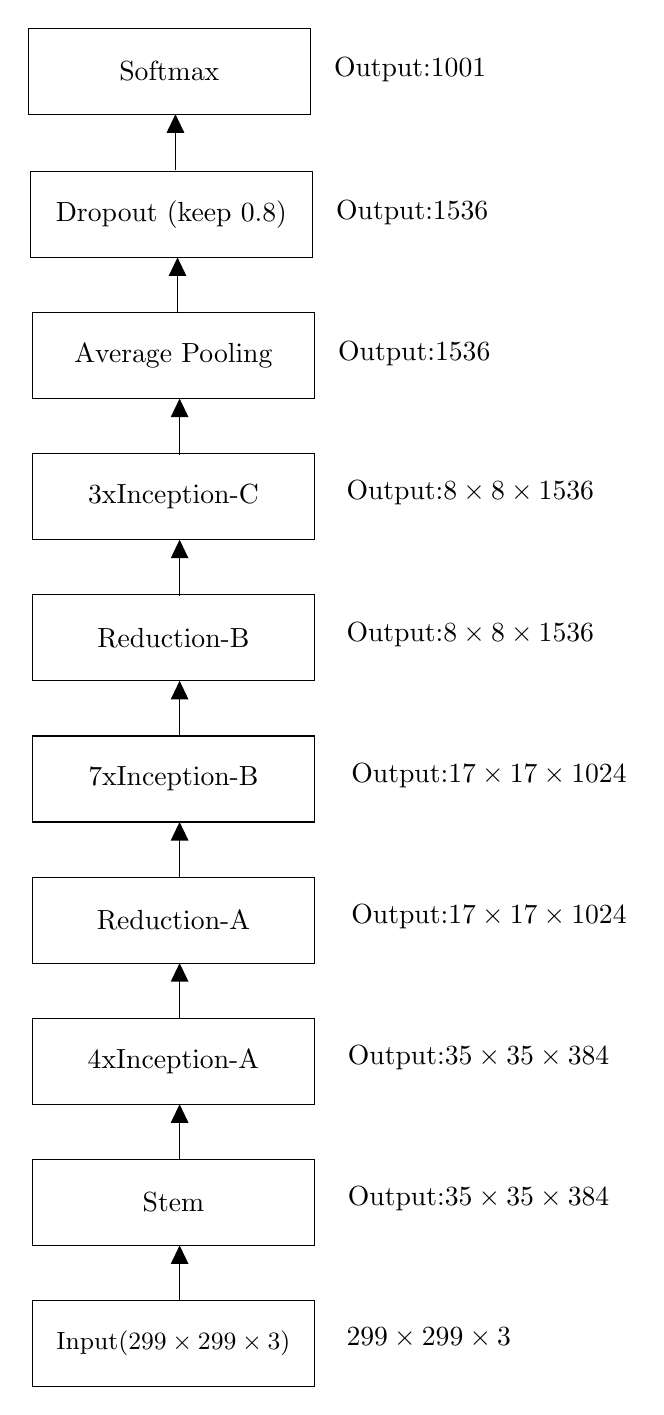
\begin{tikzpicture}[x=0.75pt,y=0.75pt,yscale=-1,xscale=1]
%uncomment if require: \path (0,742.7142868041992); %set diagram left start at 0, and has height of 742.7142868041992

%Flowchart: Process [id:dp9253173394290999] 
\draw   (98,621) -- (233.93,621) -- (233.93,662.43) -- (98,662.43) -- cycle ;
%Flowchart: Process [id:dp47578347996398307] 
\draw   (98,553) -- (233.93,553) -- (233.93,594.43) -- (98,594.43) -- cycle ;
%Straight Lines [id:da2925025767777827] 
\draw    (168.93,621.43) -- (168.93,596.43) ;
\draw [shift={(168.93,594.43)}, rotate = 450] [fill={rgb, 255:red, 0; green, 0; blue, 0 }  ][line width=0.75]  [draw opacity=0] (8.93,-4.29) -- (0,0) -- (8.93,4.29) -- cycle    ;

%Flowchart: Process [id:dp5382364848384393] 
\draw   (98,485) -- (233.93,485) -- (233.93,526.43) -- (98,526.43) -- cycle ;
%Straight Lines [id:da06940381159807729] 
\draw    (168.93,553.43) -- (168.93,528.43) ;
\draw [shift={(168.93,526.43)}, rotate = 450] [fill={rgb, 255:red, 0; green, 0; blue, 0 }  ][line width=0.75]  [draw opacity=0] (8.93,-4.29) -- (0,0) -- (8.93,4.29) -- cycle    ;

%Flowchart: Process [id:dp21301144435418706] 
\draw   (98,417) -- (233.93,417) -- (233.93,458.43) -- (98,458.43) -- cycle ;
%Straight Lines [id:da45627711718103714] 
\draw    (168.93,485.43) -- (168.93,460.43) ;
\draw [shift={(168.93,458.43)}, rotate = 450] [fill={rgb, 255:red, 0; green, 0; blue, 0 }  ][line width=0.75]  [draw opacity=0] (8.93,-4.29) -- (0,0) -- (8.93,4.29) -- cycle    ;

%Flowchart: Process [id:dp7231968775803179] 
\draw   (98,349) -- (233.93,349) -- (233.93,390.43) -- (98,390.43) -- cycle ;
%Straight Lines [id:da7165121439179447] 
\draw    (168.93,417.43) -- (168.93,392.43) ;
\draw [shift={(168.93,390.43)}, rotate = 450] [fill={rgb, 255:red, 0; green, 0; blue, 0 }  ][line width=0.75]  [draw opacity=0] (8.93,-4.29) -- (0,0) -- (8.93,4.29) -- cycle    ;

%Flowchart: Process [id:dp20620702942862734] 
\draw   (98,281) -- (233.93,281) -- (233.93,322.43) -- (98,322.43) -- cycle ;
%Straight Lines [id:da10564528480224444] 
\draw    (168.93,349.43) -- (168.93,324.43) ;
\draw [shift={(168.93,322.43)}, rotate = 450] [fill={rgb, 255:red, 0; green, 0; blue, 0 }  ][line width=0.75]  [draw opacity=0] (8.93,-4.29) -- (0,0) -- (8.93,4.29) -- cycle    ;

%Flowchart: Process [id:dp6409642010028676] 
\draw   (98,213) -- (233.93,213) -- (233.93,254.43) -- (98,254.43) -- cycle ;
%Straight Lines [id:da583110185704452] 
\draw    (168.93,281.43) -- (168.93,256.43) ;
\draw [shift={(168.93,254.43)}, rotate = 450] [fill={rgb, 255:red, 0; green, 0; blue, 0 }  ][line width=0.75]  [draw opacity=0] (8.93,-4.29) -- (0,0) -- (8.93,4.29) -- cycle    ;

%Flowchart: Process [id:dp747253235525678] 
\draw   (98,145) -- (233.93,145) -- (233.93,186.43) -- (98,186.43) -- cycle ;
%Straight Lines [id:da9482962038382927] 
\draw    (168.93,213.43) -- (168.93,188.43) ;
\draw [shift={(168.93,186.43)}, rotate = 450] [fill={rgb, 255:red, 0; green, 0; blue, 0 }  ][line width=0.75]  [draw opacity=0] (8.93,-4.29) -- (0,0) -- (8.93,4.29) -- cycle    ;

%Flowchart: Process [id:dp47103409298757426] 
\draw   (97,77) -- (232.93,77) -- (232.93,118.43) -- (97,118.43) -- cycle ;
%Straight Lines [id:da30249651940608824] 
\draw    (167.93,145.43) -- (167.93,120.43) ;
\draw [shift={(167.93,118.43)}, rotate = 450] [fill={rgb, 255:red, 0; green, 0; blue, 0 }  ][line width=0.75]  [draw opacity=0] (8.93,-4.29) -- (0,0) -- (8.93,4.29) -- cycle    ;

%Flowchart: Process [id:dp5661311837160838] 
\draw   (96,8) -- (231.93,8) -- (231.93,49.43) -- (96,49.43) -- cycle ;
%Straight Lines [id:da5142446239913938] 
\draw    (166.93,76.43) -- (166.93,51.43) ;
\draw [shift={(166.93,49.43)}, rotate = 450] [fill={rgb, 255:red, 0; green, 0; blue, 0 }  ][line width=0.75]  [draw opacity=0] (8.93,-4.29) -- (0,0) -- (8.93,4.29) -- cycle    ;


% Text Node
\draw (165.96,641.71) node  [align=left] {{\small Input($\displaystyle 299\times 299\times 3$)}};
% Text Node
\draw (165.96,573.71) node  [align=left] {Stem};
% Text Node
\draw (289,639) node  [align=left] {$\displaystyle 299\times 299\times 3$};
% Text Node
\draw (313,572) node  [align=left] {Output:$\displaystyle 35\times 35\times 384$};
% Text Node
\draw (165.96,505.71) node  [align=left] {4xInception-A};
% Text Node
\draw (313,504) node  [align=left] {Output:$\displaystyle 35\times 35\times 384$};
% Text Node
\draw (165.96,437.71) node  [align=left] {Reduction-A};
% Text Node
\draw (318,436) node  [align=left] {Output:$\displaystyle 17\times 17\times 1024$};
% Text Node
\draw (165.96,369.71) node  [align=left] {7xInception-B};
% Text Node
\draw (318,368) node  [align=left] {Output:$\displaystyle 17\times 17\times 1024$};
% Text Node
\draw (165.96,301.71) node  [align=left] {Reduction-B};
% Text Node
\draw (309,300) node  [align=left] {Output:$\displaystyle 8\times 8\times 1536$};
% Text Node
\draw (165.96,233.71) node  [align=left] {3xInception-C};
% Text Node
\draw (309,232) node  [align=left] {Output:$\displaystyle 8\times 8\times 1536$};
% Text Node
\draw (165.96,165.71) node  [align=left] {Average Pooling};
% Text Node
\draw (282,165) node  [align=left] {Output:$\displaystyle 1536$};
% Text Node
\draw (164.96,97.71) node  [align=left] {Dropout (keep $\displaystyle 0.8$)};
% Text Node
\draw (281,97) node  [align=left] {Output:$\displaystyle 1536$};
% Text Node
\draw (163.96,28.71) node  [align=left] {Softmax};
% Text Node
\draw (280,28) node  [align=left] {Output:$\displaystyle 1001$};


\end{tikzpicture}}
   \caption{InceptionV4 architecture \cite{InceptionV4}}
   \label{fig:inceptionv4Archi} 
\end{subfigure}%
\begin{subfigure}[t]{0.47\textwidth}
   %%Verify the architectures again
   \resizebox{.99\linewidth}{!}{

\tikzset{every picture/.style={line width=0.75pt}} %set default line width to 0.75pt        

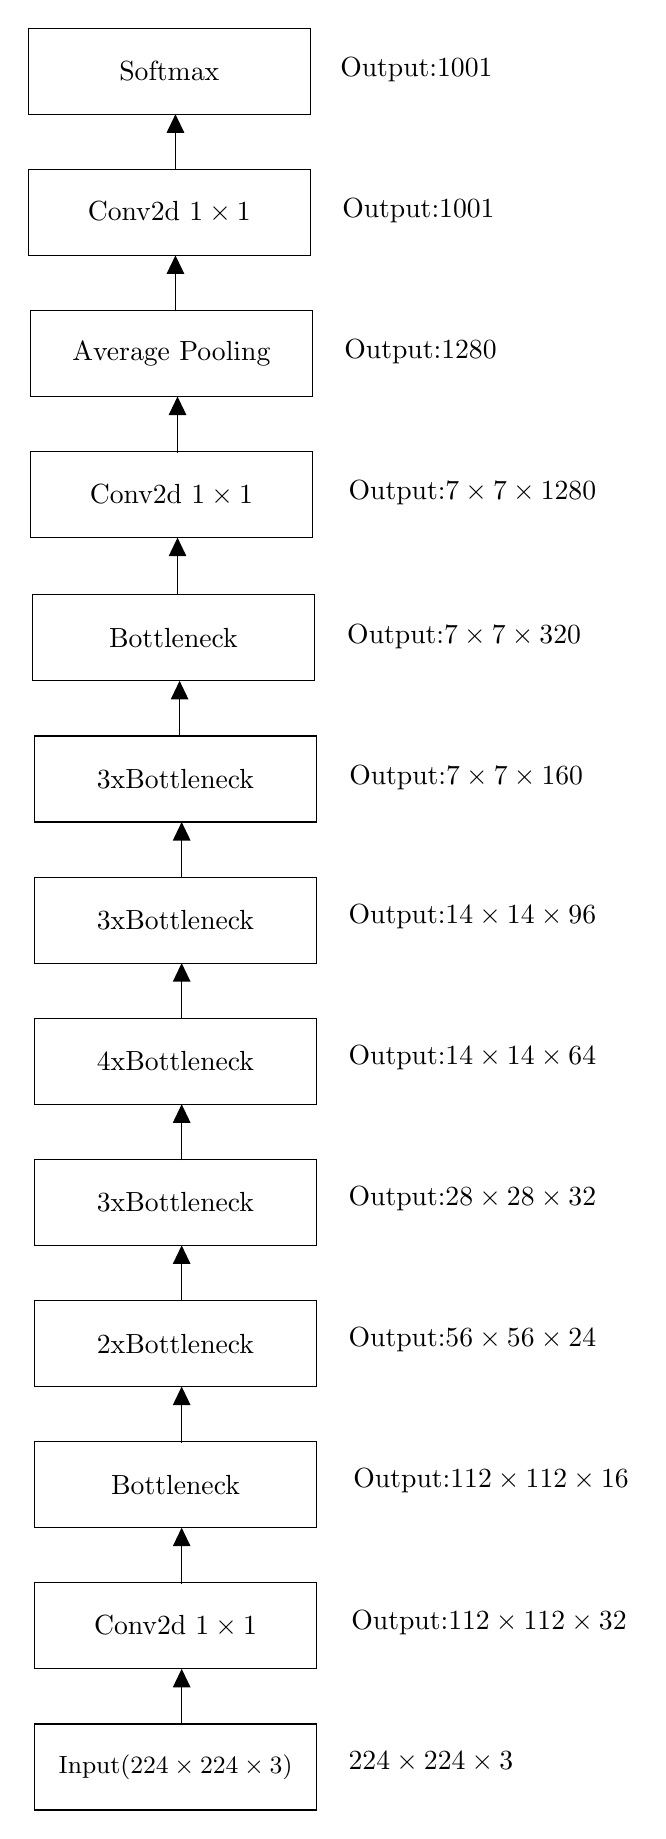
\begin{tikzpicture}[x=0.75pt,y=0.75pt,yscale=-1,xscale=1]
%uncomment if require: \path (0,948.6666870117188); %set diagram left start at 0, and has height of 948.6666870117188

%Flowchart: Process [id:dp9253173394290999] 
\draw   (98,897) -- (233.93,897) -- (233.93,938.43) -- (98,938.43) -- cycle ;
%Flowchart: Process [id:dp47578347996398307] 
\draw   (98,829) -- (233.93,829) -- (233.93,870.43) -- (98,870.43) -- cycle ;
%Straight Lines [id:da2925025767777827] 
\draw    (168.93,897.43) -- (168.93,872.43) ;
\draw [shift={(168.93,870.43)}, rotate = 450] [fill={rgb, 255:red, 0; green, 0; blue, 0 }  ][line width=0.75]  [draw opacity=0] (8.93,-4.29) -- (0,0) -- (8.93,4.29) -- cycle    ;

%Flowchart: Process [id:dp5382364848384393] 
\draw   (98,761) -- (233.93,761) -- (233.93,802.43) -- (98,802.43) -- cycle ;
%Straight Lines [id:da06940381159807729] 
\draw    (168.93,829.43) -- (168.93,804.43) ;
\draw [shift={(168.93,802.43)}, rotate = 450] [fill={rgb, 255:red, 0; green, 0; blue, 0 }  ][line width=0.75]  [draw opacity=0] (8.93,-4.29) -- (0,0) -- (8.93,4.29) -- cycle    ;

%Flowchart: Process [id:dp21301144435418706] 
\draw   (98,693) -- (233.93,693) -- (233.93,734.43) -- (98,734.43) -- cycle ;
%Straight Lines [id:da45627711718103714] 
\draw    (168.93,761.43) -- (168.93,736.43) ;
\draw [shift={(168.93,734.43)}, rotate = 450] [fill={rgb, 255:red, 0; green, 0; blue, 0 }  ][line width=0.75]  [draw opacity=0] (8.93,-4.29) -- (0,0) -- (8.93,4.29) -- cycle    ;

%Flowchart: Process [id:dp7231968775803179] 
\draw   (98,625) -- (233.93,625) -- (233.93,666.43) -- (98,666.43) -- cycle ;
%Straight Lines [id:da7165121439179447] 
\draw    (168.93,693.43) -- (168.93,668.43) ;
\draw [shift={(168.93,666.43)}, rotate = 450] [fill={rgb, 255:red, 0; green, 0; blue, 0 }  ][line width=0.75]  [draw opacity=0] (8.93,-4.29) -- (0,0) -- (8.93,4.29) -- cycle    ;

%Flowchart: Process [id:dp20620702942862734] 
\draw   (98,557) -- (233.93,557) -- (233.93,598.43) -- (98,598.43) -- cycle ;
%Straight Lines [id:da10564528480224444] 
\draw    (168.93,625.43) -- (168.93,600.43) ;
\draw [shift={(168.93,598.43)}, rotate = 450] [fill={rgb, 255:red, 0; green, 0; blue, 0 }  ][line width=0.75]  [draw opacity=0] (8.93,-4.29) -- (0,0) -- (8.93,4.29) -- cycle    ;

%Flowchart: Process [id:dp6409642010028676] 
\draw   (98,489) -- (233.93,489) -- (233.93,530.43) -- (98,530.43) -- cycle ;
%Straight Lines [id:da583110185704452] 
\draw    (168.93,557.43) -- (168.93,532.43) ;
\draw [shift={(168.93,530.43)}, rotate = 450] [fill={rgb, 255:red, 0; green, 0; blue, 0 }  ][line width=0.75]  [draw opacity=0] (8.93,-4.29) -- (0,0) -- (8.93,4.29) -- cycle    ;

%Flowchart: Process [id:dp747253235525678] 
\draw   (98,421) -- (233.93,421) -- (233.93,462.43) -- (98,462.43) -- cycle ;
%Straight Lines [id:da9482962038382927] 
\draw    (168.93,489.43) -- (168.93,464.43) ;
\draw [shift={(168.93,462.43)}, rotate = 450] [fill={rgb, 255:red, 0; green, 0; blue, 0 }  ][line width=0.75]  [draw opacity=0] (8.93,-4.29) -- (0,0) -- (8.93,4.29) -- cycle    ;

%Flowchart: Process [id:dp47103409298757426] 
\draw   (97,353) -- (232.93,353) -- (232.93,394.43) -- (97,394.43) -- cycle ;
%Straight Lines [id:da30249651940608824] 
\draw    (167.93,421.43) -- (167.93,396.43) ;
\draw [shift={(167.93,394.43)}, rotate = 450] [fill={rgb, 255:red, 0; green, 0; blue, 0 }  ][line width=0.75]  [draw opacity=0] (8.93,-4.29) -- (0,0) -- (8.93,4.29) -- cycle    ;

%Flowchart: Process [id:dp5661311837160838] 
\draw   (96,284) -- (231.93,284) -- (231.93,325.43) -- (96,325.43) -- cycle ;
%Straight Lines [id:da5142446239913938] 
\draw    (166.93,352.43) -- (166.93,327.43) ;
\draw [shift={(166.93,325.43)}, rotate = 450] [fill={rgb, 255:red, 0; green, 0; blue, 0 }  ][line width=0.75]  [draw opacity=0] (8.93,-4.29) -- (0,0) -- (8.93,4.29) -- cycle    ;

%Flowchart: Process [id:dp8648151912409288] 
\draw   (96,216) -- (231.93,216) -- (231.93,257.43) -- (96,257.43) -- cycle ;
%Straight Lines [id:da21788225541174455] 
\draw    (166.93,284.43) -- (166.93,259.43) ;
\draw [shift={(166.93,257.43)}, rotate = 450] [fill={rgb, 255:red, 0; green, 0; blue, 0 }  ][line width=0.75]  [draw opacity=0] (8.93,-4.29) -- (0,0) -- (8.93,4.29) -- cycle    ;

%Flowchart: Process [id:dp5915277931570215] 
\draw   (95,148) -- (230.93,148) -- (230.93,189.43) -- (95,189.43) -- cycle ;
%Straight Lines [id:da2169186042376452] 
\draw    (165.93,216.43) -- (165.93,191.43) ;
\draw [shift={(165.93,189.43)}, rotate = 450] [fill={rgb, 255:red, 0; green, 0; blue, 0 }  ][line width=0.75]  [draw opacity=0] (8.93,-4.29) -- (0,0) -- (8.93,4.29) -- cycle    ;

%Flowchart: Process [id:dp09241683513730559] 
\draw   (95,80) -- (230.93,80) -- (230.93,121.43) -- (95,121.43) -- cycle ;
%Straight Lines [id:da3985231842573671] 
\draw    (165.93,148.43) -- (165.93,123.43) ;
\draw [shift={(165.93,121.43)}, rotate = 450] [fill={rgb, 255:red, 0; green, 0; blue, 0 }  ][line width=0.75]  [draw opacity=0] (8.93,-4.29) -- (0,0) -- (8.93,4.29) -- cycle    ;


% Text Node
\draw (165.96,917.71) node  [align=left] {{\small Input($\displaystyle 224\times 224\times 3$)}};
% Text Node
\draw (165.96,849.71) node  [align=left] {Conv2d $\displaystyle 1\times 1$};
% Text Node
\draw (289,915) node  [align=left] {$\displaystyle 224\times 224\times 3$};
% Text Node
\draw (317,848) node  [align=left] {Output:$\displaystyle 112\times 112\times 32$};
% Text Node
\draw (165.96,781.71) node  [align=left] {Bottleneck};
% Text Node
\draw (318,780) node  [align=left] {Output:$\displaystyle 112\times 112\times 16$};
% Text Node
\draw (165.96,713.71) node  [align=left] {2xBottleneck};
% Text Node
\draw (309,712) node  [align=left] {Output:$\displaystyle 56\times 56\times 24$};
% Text Node
\draw (165.96,645.71) node  [align=left] {3xBottleneck};
% Text Node
\draw (309,644) node  [align=left] {Output:$\displaystyle 28\times 28\times 32$};
% Text Node
\draw (165.96,577.71) node  [align=left] {4xBottleneck};
% Text Node
\draw (309,576) node  [align=left] {Output:$\displaystyle 14\times 14\times 64$};
% Text Node
\draw (165.96,509.71) node  [align=left] {3xBottleneck};
% Text Node
\draw (309,508) node  [align=left] {Output:$\displaystyle 14\times 14\times 96$};
% Text Node
\draw (165.96,441.71) node  [align=left] {3xBottleneck};
% Text Node
\draw (306,441) node  [align=left] {Output:$\displaystyle 7\times 7\times 160$};
% Text Node
\draw (164.96,373.71) node  [align=left] {Bottleneck};
% Text Node
\draw (305,373) node  [align=left] {Output:$\displaystyle 7\times 7\times 320$};
% Text Node
\draw (163.96,304.71) node  [align=left] {Conv2d $\displaystyle 1\times 1$};
% Text Node
\draw (309,304) node  [align=left] {Output:$\displaystyle 7\times 7\times 1280$};
% Text Node
\draw (163.96,236.71) node  [align=left] {Average Pooling};
% Text Node
\draw (284,236) node  [align=left] {Output:$\displaystyle 1280$};
% Text Node
\draw (162.96,168.71) node  [align=left] {Conv2d $\displaystyle 1\times 1$};
% Text Node
\draw (283,168) node  [align=left] {Output:$\displaystyle 1001$};
% Text Node
\draw (162.96,100.71) node  [align=left] {Softmax};
% Text Node
\draw (282,100) node  [align=left] {Output:$\displaystyle 1001$};


\end{tikzpicture}}
   \caption{MobileNetV2 architecture \cite{DBLP:journals/corr/abs-1801-04381}}
   \label{fig:MobileNetArchi}
\end{subfigure}

\caption{Architectures of InceptionV4 and MobileNetV2}
%%NO DROPOUT AT INFERENCE
\end{figure}



\subsection{Android Benchmark Application}
\label{chap:androidApp}
To conduct the experiments for both edge and cloud inference we developed and implemented an Android benchmark application using Kotlin.
This application implements all function needed to preprocess real workload images and perform the inference on either the Android device itself or sent the image to a cloud-backend.
For both preprocessing and inference the application logs metrics such as inference latency, time of the experiments etc. and stores them to a \emph{CSV} file, which then can be used to evaluation purposes.

Both edge and cloud inference implementations are based on the example implementations in the respective GitHub repositories to ensure optimal performance. 


\begin{figure}[htb]
\centering
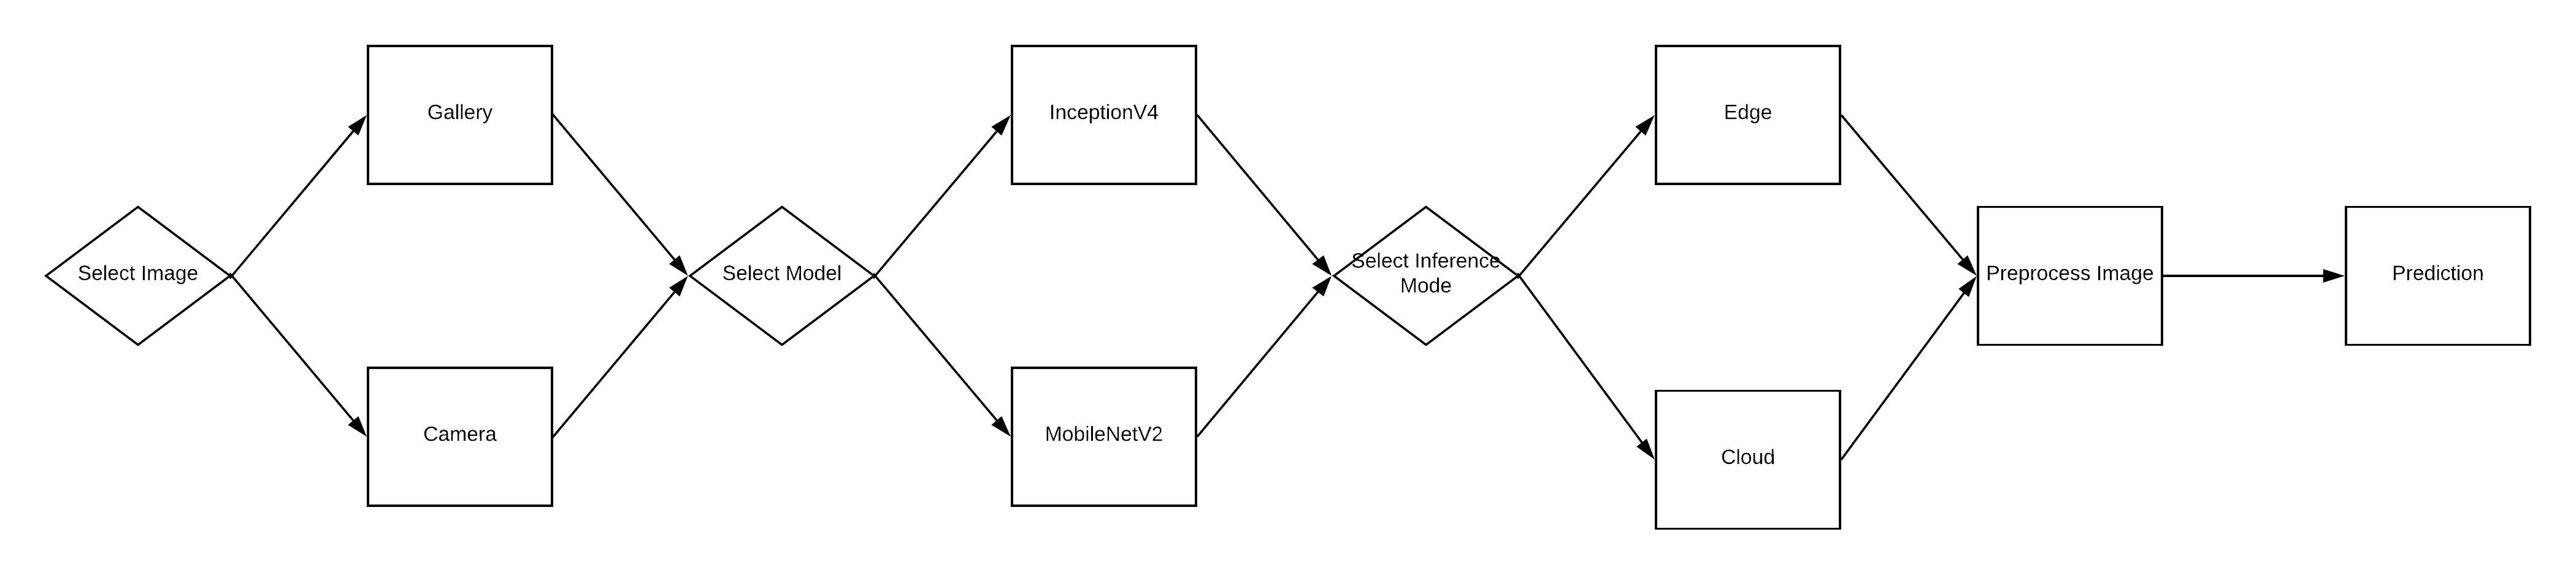
\includegraphics[width=0.97\textwidth]{./Bilder/FlowChart_App.png}
\caption{Flowchart of the Benchmark Application}
\label{fig:app}
\end{figure}
In figure \ref{fig:app} the work-flow to perform the inference is seen. First, a image needs to be selected. Afterwards the image classification model needs to be chosen. Now the user selects whether the inference should be performed on the cloud-backend or directly on the edge device, in this case a Android phone. In the case of edge inference it needs to be decided if the NNAPI should be used by TensorFlow Lite. For cloud inference the preprocessing mode needs to be selected (edge/cloud). Now the preprocessing operations can be performed based on the previous selected options (Even for the case of cloud inference with cloud preprocessing some preprocessing needs to be done on the edge beforehand like building a \emph{PredictRequest} containing the request for the cloud-backend). Now, that the input is preprocessed, the actual inference is performed as a last step, resulting in a prediction. For both preprocessing and inference the measurements mentioned in section \ref{chap:insta_measurements} are logged.

\begin{figure}[htb]
\centering
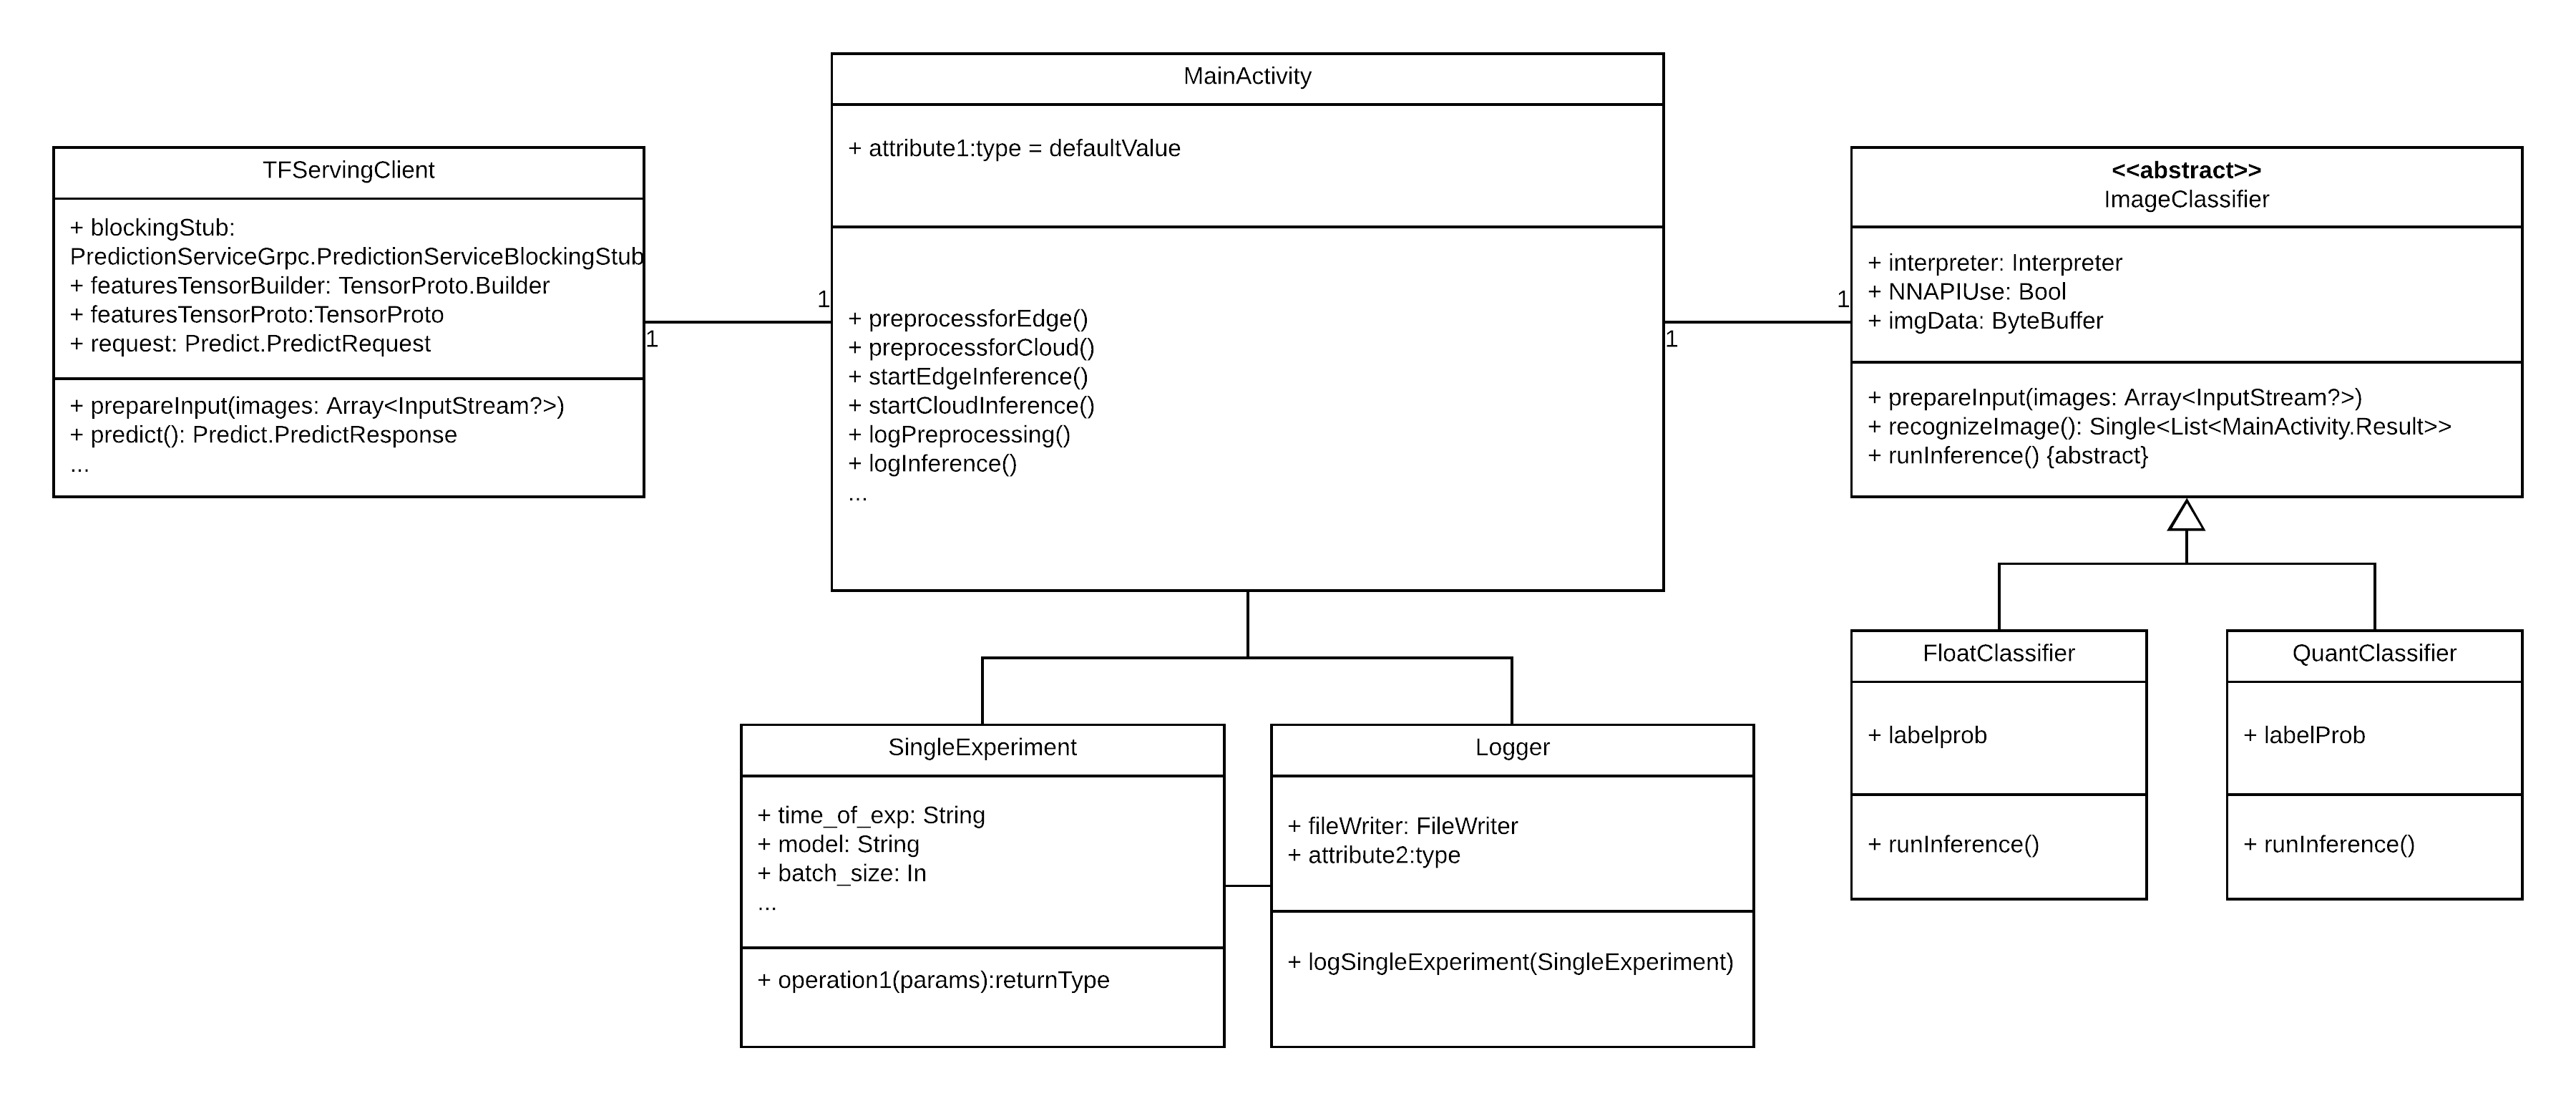
\includegraphics[width=0.99\textwidth]{./Bilder/UML.png}
\caption{UML class diagram of the benchmark application}
\label{fig:UML}
\end{figure}
Figure \ref{fig:UML} depicts an UML class diagram of the application featuring the most important classes, functions and variables. 
The main class is called \emph{MainActivity} and implements all of the graphical aspects. 
The \emph{MainActivity} handles requests for both cloud and edge inference by delegating the requests to instances of the classes \emph{TFServingClient} and \emph{ImageClassifier}, respectively. Both of these classes also take care of the preprocessing steps.
The abstract class \emph{ImageClassifier} has two subclasses \emph{FloatClassifier} and \emph{QuantClassifier}. The first class runs the inference for floating point models and the second for quantized models.
This separation is needed since these different model types require different input and output types.

The \emph{MainActivity} writes the collected measurements and the parameter configurations of an experiment to a instance of \emph{SingleExperiment}. After the experiment is completed \emph{MainActivity} tells a \emph{Logger} instance to save the contents of the \emph{SingleExperiment} object. The Logger then saves all collected data to a \emph{CSV} file.

\subsubsection{Preprocessing}
%%mention png
For the case of image classification, the images need to have the correct size ($224\times224$ for MobilenetV2 and $299\times299$ for InceptionV4) and the RGB values need to be normalized to the interval $[-1,1]$. After preprocessing the image has been transformed into the shape $224\times224\times3$ with all values between $[-1,1]$, where the the first two dimensions represent the image height and width, while the last dimension represent the number of channels (3 since the images are RGB)
\begin{figure}[H]
\centering


\tikzset{every picture/.style={line width=0.75pt}} %set default line width to 0.75pt        

\begin{tikzpicture}[x=0.75pt,y=0.75pt,yscale=-1,xscale=1]
%uncomment if require: \path (0,484.3333282470703); %set diagram left start at 0, and has height of 484.3333282470703

%Shape: Square [id:dp1081653036325061] 
\draw  [fill={rgb, 255:red, 0; green, 0; blue, 255 }  ,fill opacity=1 ] (217.67,92) -- (317,92) -- (317,191.33) -- (217.67,191.33) -- cycle ;
%Shape: Square [id:dp8785233930816818] 
\draw  [fill={rgb, 255:red, 0; green, 255; blue, 0 }  ,fill opacity=1 ] (207.67,100) -- (307,100) -- (307,199.33) -- (207.67,199.33) -- cycle ;
%Image [id:dp7451570314710638] 
\draw (67,158.49) node  {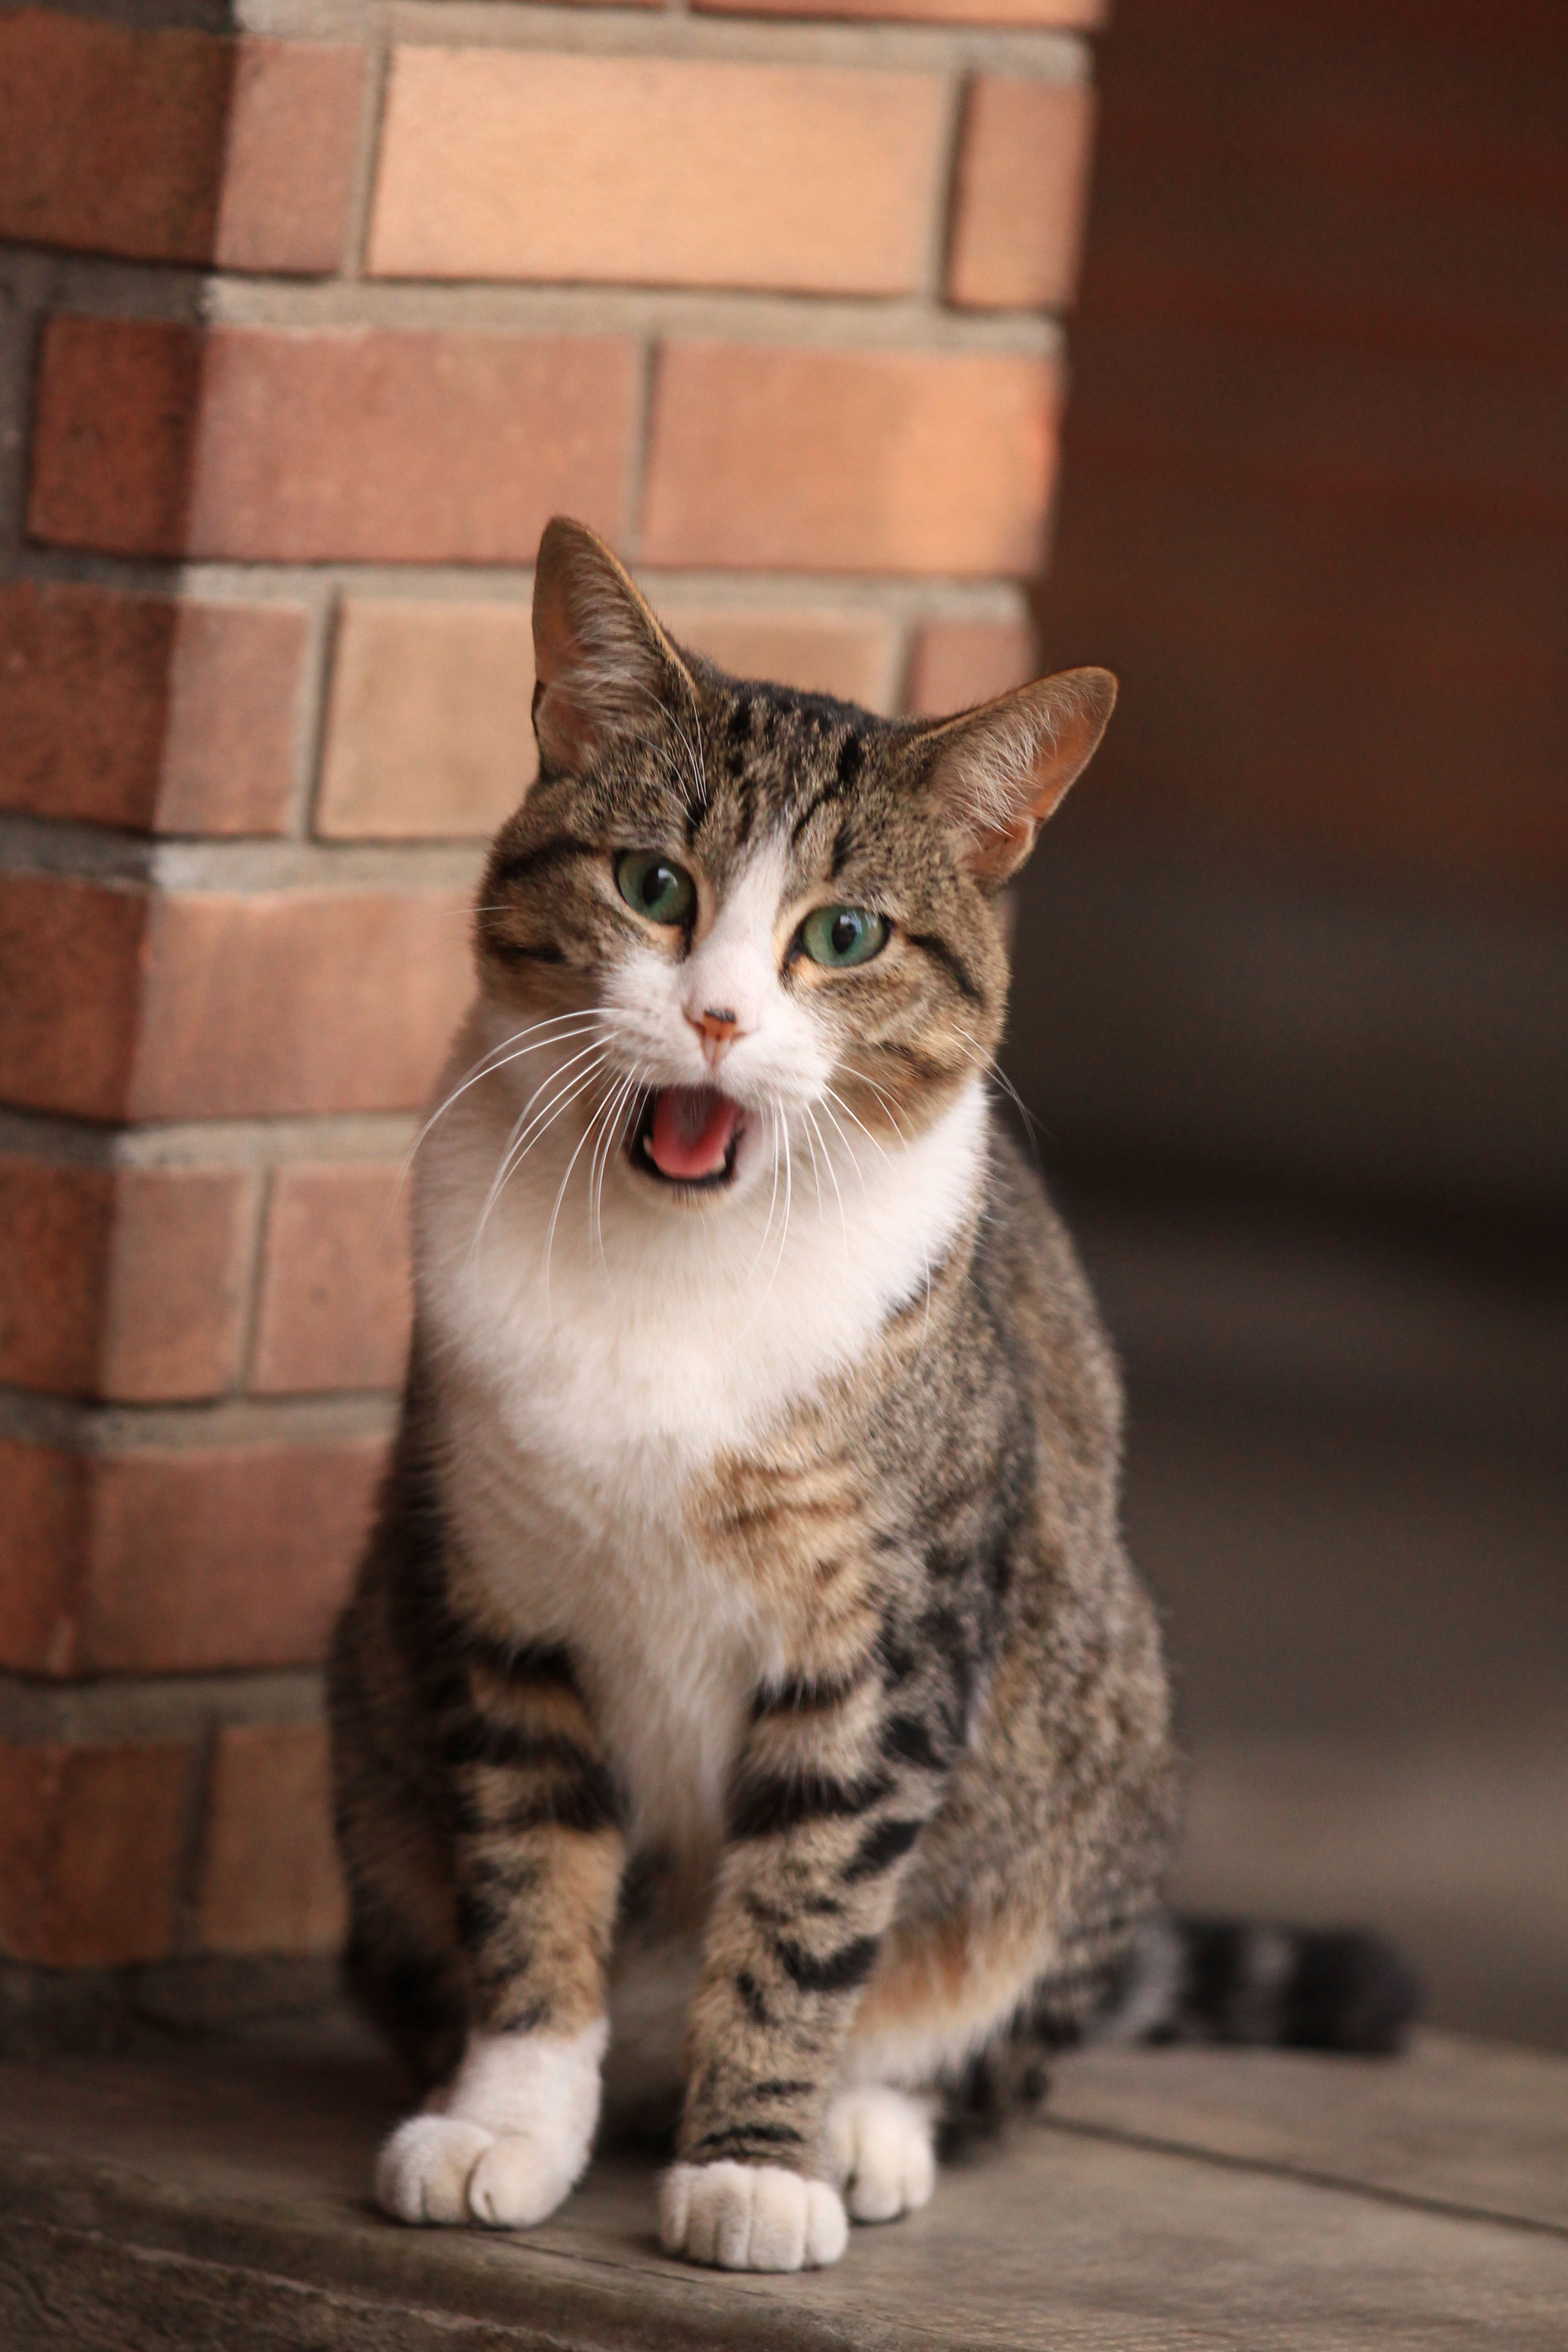
\includegraphics[width=52.5pt,height=78.73pt]{Bilder/European_cat_02_16_mp.jpg}};
%Shape: Square [id:dp7219434207477922] 
\draw  [fill={rgb, 255:red, 255; green, 0; blue, 0 }  ,fill opacity=1 ] (199.67,110) -- (299,110) -- (299,209.33) -- (199.67,209.33) -- cycle ;
%Straight Lines [id:da9021822569380376] 
\draw    (106.17,157.33) -- (177.17,157.33) ;
\draw [shift={(179.17,157.33)}, rotate = 180] [fill={rgb, 255:red, 0; green, 0; blue, 0 }  ][line width=0.75]  [draw opacity=0] (8.93,-4.29) -- (0,0) -- (8.93,4.29) -- cycle    ;

%Straight Lines [id:da9159956987115614] 
\draw    (337.17,157.33) -- (408.17,157.33) ;
\draw [shift={(410.17,157.33)}, rotate = 180] [fill={rgb, 255:red, 0; green, 0; blue, 0 }  ][line width=0.75]  [draw opacity=0] (8.93,-4.29) -- (0,0) -- (8.93,4.29) -- cycle    ;

%Straight Lines [id:da07325949392344144] 
\draw  [dash pattern={on 0.84pt off 2.51pt}]  (232.17,121.33) -- (277.17,121.33) ;


%Straight Lines [id:da9028616351053764] 
\draw  [dash pattern={on 0.84pt off 2.51pt}]  (233.17,196.33) -- (278.17,196.33) ;


%Straight Lines [id:da27535102010063794] 
\draw  [dash pattern={on 0.84pt off 2.51pt}]  (217.17,136.33) -- (217.17,184.33) ;


%Straight Lines [id:da9334949593538635] 
\draw  [dash pattern={on 0.84pt off 2.51pt}]  (286.17,133.33) -- (286.17,181.33) ;


%Straight Lines [id:da021722670153532242] 
\draw  [dash pattern={on 0.84pt off 2.51pt}]  (228.17,131.33) -- (278.17,183.33) ;


%Shape: Square [id:dp4109817022076603] 
\draw  [fill={rgb, 255:red, 255; green, 255; blue, 255 }  ,fill opacity=1 ] (449.67,90) -- (549,90) -- (549,189.33) -- (449.67,189.33) -- cycle ;
%Shape: Square [id:dp544671777438523] 
\draw  [fill={rgb, 255:red, 255; green, 255; blue, 255 }  ,fill opacity=1 ] (439.67,98) -- (539,98) -- (539,197.33) -- (439.67,197.33) -- cycle ;
%Shape: Square [id:dp9050599364199439] 
\draw  [fill={rgb, 255:red, 255; green, 255; blue, 255 }  ,fill opacity=1 ] (431.67,108) -- (531,108) -- (531,207.33) -- (431.67,207.33) -- cycle ;
%Straight Lines [id:da02360170094364733] 
\draw  [dash pattern={on 0.84pt off 2.51pt}]  (455.17,120.33) -- (500.17,120.33) ;


%Straight Lines [id:da10167634289204797] 
\draw  [dash pattern={on 0.84pt off 2.51pt}]  (455.17,194.33) -- (500.17,194.33) ;


%Straight Lines [id:da23003293896688182] 
\draw  [dash pattern={on 0.84pt off 2.51pt}]  (443.17,135.33) -- (443.17,183.33) ;


%Straight Lines [id:da28496973593396335] 
\draw  [dash pattern={on 0.84pt off 2.51pt}]  (521.17,134.33) -- (521.17,182.33) ;


%Straight Lines [id:da06739883279353798] 
\draw  [dash pattern={on 0.84pt off 2.51pt}]  (452.17,127.33) -- (514.17,183.33) ;



% Text Node
\draw (250,217) node  [align=left] {$\displaystyle 224$};
% Text Node
\draw (188.17,157.33) node [rotate=-270] [align=left] {$\displaystyle 224$};
% Text Node
\draw (314,202) node [rotate=-319.82] [align=left] {$\displaystyle 3$};
% Text Node
\draw (141,170) node  [align=left] {Resizing};
% Text Node
\draw (371,171) node  [align=left] {Normalization};
% Text Node
\draw (215.67,197.33) node  [align=left] {$\displaystyle 255$};
% Text Node
\draw (216,120) node  [align=left] {$\displaystyle 255$};
% Text Node
\draw (287,196) node  [align=left] {$\displaystyle 0$};
% Text Node
\draw (286,120) node  [align=left] {$\displaystyle 0$};
% Text Node
\draw (442.67,194.33) node  [align=left] {$\displaystyle 1$};
% Text Node
\draw (444,118) node  [align=left] {$\displaystyle 1$};
% Text Node
\draw (519,193) node  [align=left] {$\displaystyle -1$};
% Text Node
\draw (518,118) node  [align=left] {$\displaystyle -1$};
% Text Node
\draw (421.17,155.33) node [rotate=-270] [align=left] {$\displaystyle 224$};
% Text Node
\draw (484,215) node  [align=left] {$\displaystyle 224$};
% Text Node
\draw (546,203) node [rotate=-319.82] [align=left] {$\displaystyle 3$};
% Text Node
\draw (67,220) node  [align=left] {$\displaystyle 1633$};
% Text Node
\draw (22,153) node [rotate=-270.5] [align=left] {$\displaystyle 2449$};
% Text Node
\draw (69,98) node  [align=left] {{\scriptsize source: [SeL] }};


\end{tikzpicture}
\caption{Preprocessing steps for image classifcation}
\label{fig:prepro}
\end{figure}
\paragraph{Edge Preprocessing}
In the case of edge preprocessing all preprocessing steps are done on the edge device, meaning that the input can be fed directly into the neural network afterwards, either on the edge device itself or on a cloud-backend.
We perform these steps the following way: After loading the PNG image into an \emph{InputStream} we create a scaled Bitmap of the image (scaled to either $224\times224$ or $299\times299$) by calling the \emph{createScaledBitmap} function. 
Afterwards we normalize the RGB values to $[-1,1]$ during the conversion from the bitmap to a \emph{ByteBuffer}. 
For the case of float models this buffer contains all the pixels in float format and for quantized model in bytes, since quantized models work with lower represenations.
%%%mehr erklären?
We do this conversion since feeding \emph{ByteBuffers} to TensorFlow Lite is performance enhancing. %add cite here
For cloud inference we then construct \emph{PredictRequest} object containing this \emph{ByteBuffer}.

For batch size larger than one we parallize the preprocessing to speed up the proprocessing latency at the cost of higher maximum memory consumption. We start $n$ threads, where each thread is preprocessing one image in the way described above. After each image is preprocessed we concatenate all \emph{ByteBuffers} into a single one, which then can be fed to the TensorFlow Lite interpreter. Note that $n$ is determined by both batch size and available CPU cores on the edge device. There are never more threads than available cores, but if the batch size is smaller than the number of cores, we only start $n$ threads, where $n$ is the batch size. 

\paragraph{Cloud Preprocessing}

In the case of cloud inference the images can also be preprocessed directly on the cloud, resulting in nearly no preprocessing done on the edge. While the resizing and scaling steps are no longer done on the edge, the image still needs to converted into a \emph{PredictRequest} object that TensorFlow Serving can handle.
To achieve this we again load the PNG image into an \emph{InputStream}, convert it to a \emph{ByteArray} which then can be feed to the \emph{PredictRequest} object as a \emph{ByteString}. 

%Add TensorFlow Serving preprocessing here


\subsubsection{Inference}
To get the predictions for our now preprocessed image we need to run the inference operation of the inference framework with the deep learning model laoded, which is loaded either directly on the edge or on the remote cloud-backend. 
The inference is done using the steps described in section \ref{chap:TFLite} (TensorFlow Lite) and \ref{chap:TFServing} (TensorFlow Serving).
\paragraph{Edge Inference}
To perform the inference operation we two things into the \emph{run} function of an interpreter of TensorFlow Lite: The \emph{ByteBuffer} created in the preprocessing step and an array (float models: \emph{FloatArray}, quantized models: \emph{ByteArray}) with the length 1001 (number of classes). TensorFlow lite then writes the confidence levels of the different classes to this array. We then sort the array for the five classes with the highest confidence and print them to the screen.

\paragraph{Cloud Inference}

For the cloud inference we send the \emph{PredictRequest} object created in the preprocessing process to the TensorFlow Serving server, where the inference (and in the case of cloud preprocessing also the preprocessing) computations are executed.
To sent the \emph{PredictRequest} object to the server we call the \emph{predict} function of the previous created TensorFlow Serving gRPC stub.
Afterwards the client receives the \emph{PredictResponse} from the server containing the predictions for the sent image. We configured the TensorFlow Serving models to return the five classes with the highest confidence, hence we extract these five classes from the \emph{PredictResponse} and print them to the screen.

To preprocess the image on the cloud we add TensorFlows preprocessing functions to the model graphs before we export them to the TensorFlow Serving format. The images arrive at the server in the \emph{PNG} format, therefore we first decode them with \emph{tf.image.decode\_jpeg}, then resize with \emph{tf.image.resize\_bilinear} and finally normalize the tensor values to $[-1,1]$ using the the \emph{subtract} and \emph{multiply} functions. Now the input has the same shape as if they would have been preprocessed on the edge can be fed to the actual model graphs.
\section{Instantiation}
Using the experimental design presented in the previous section, we now describe which parameters we change in the course of the experiments as well as how the performance metrics are measured.
\subsection{Parameters}
We run each parameter configuration 15 times to reduce variance and stabilize our results.
During the experiments no other applications are running on either the edge or the cloud device.
In the course of the experiments we change the configurations of the following parameters:
%%%293,performance analysis buch
\paragraph{Model}
We conduct experiments for all three models listed presented in \ref{chap:models}: InceptionV4, MobileNetV2 and MobileNetV2 quantized.

\paragraph{Preprocessing Mode}
For the case of cloud inference the major parts of the needed preprocessing is either done on the edge before sending the image to the cloud or done on cloud. Therefore we evaluate both options.
\paragraph{Inference Mode}
The inference can either be performed on the edge or an a cloud-backend.

\paragraph{Image Size}
%%Add table here?
%224: 83KB
%299: 141KB
%2MP: 2411KB
%4MP: 4309KB
%8MP: 7515KB
%16MP: 10077KB
We evaluate the performance of 2MP($1732\times1155$, $2411$KB), 4MP($2449\times1633$, $4309$KB), 8MP($3464\times2309$, $7515$KB) and 16MP($4899\times3266$, $10077$KB) PNG images, as the OnePlus 6T is capable of taking pictures with 16 megapixel. This way the effect of different image sizes on the performance of the preprocessing step can assessed. We also evaluate an image where no resizing is needed ($224\times224$, $83$KB or $299\times299$, $141$KB depending on the model) to study the impact of image resizing. A picture of a cat (see figure \ref{fig:cat}) scaled to the different sizes will serve as the picture for the experiments.
\begin{figure}[H]
\centering
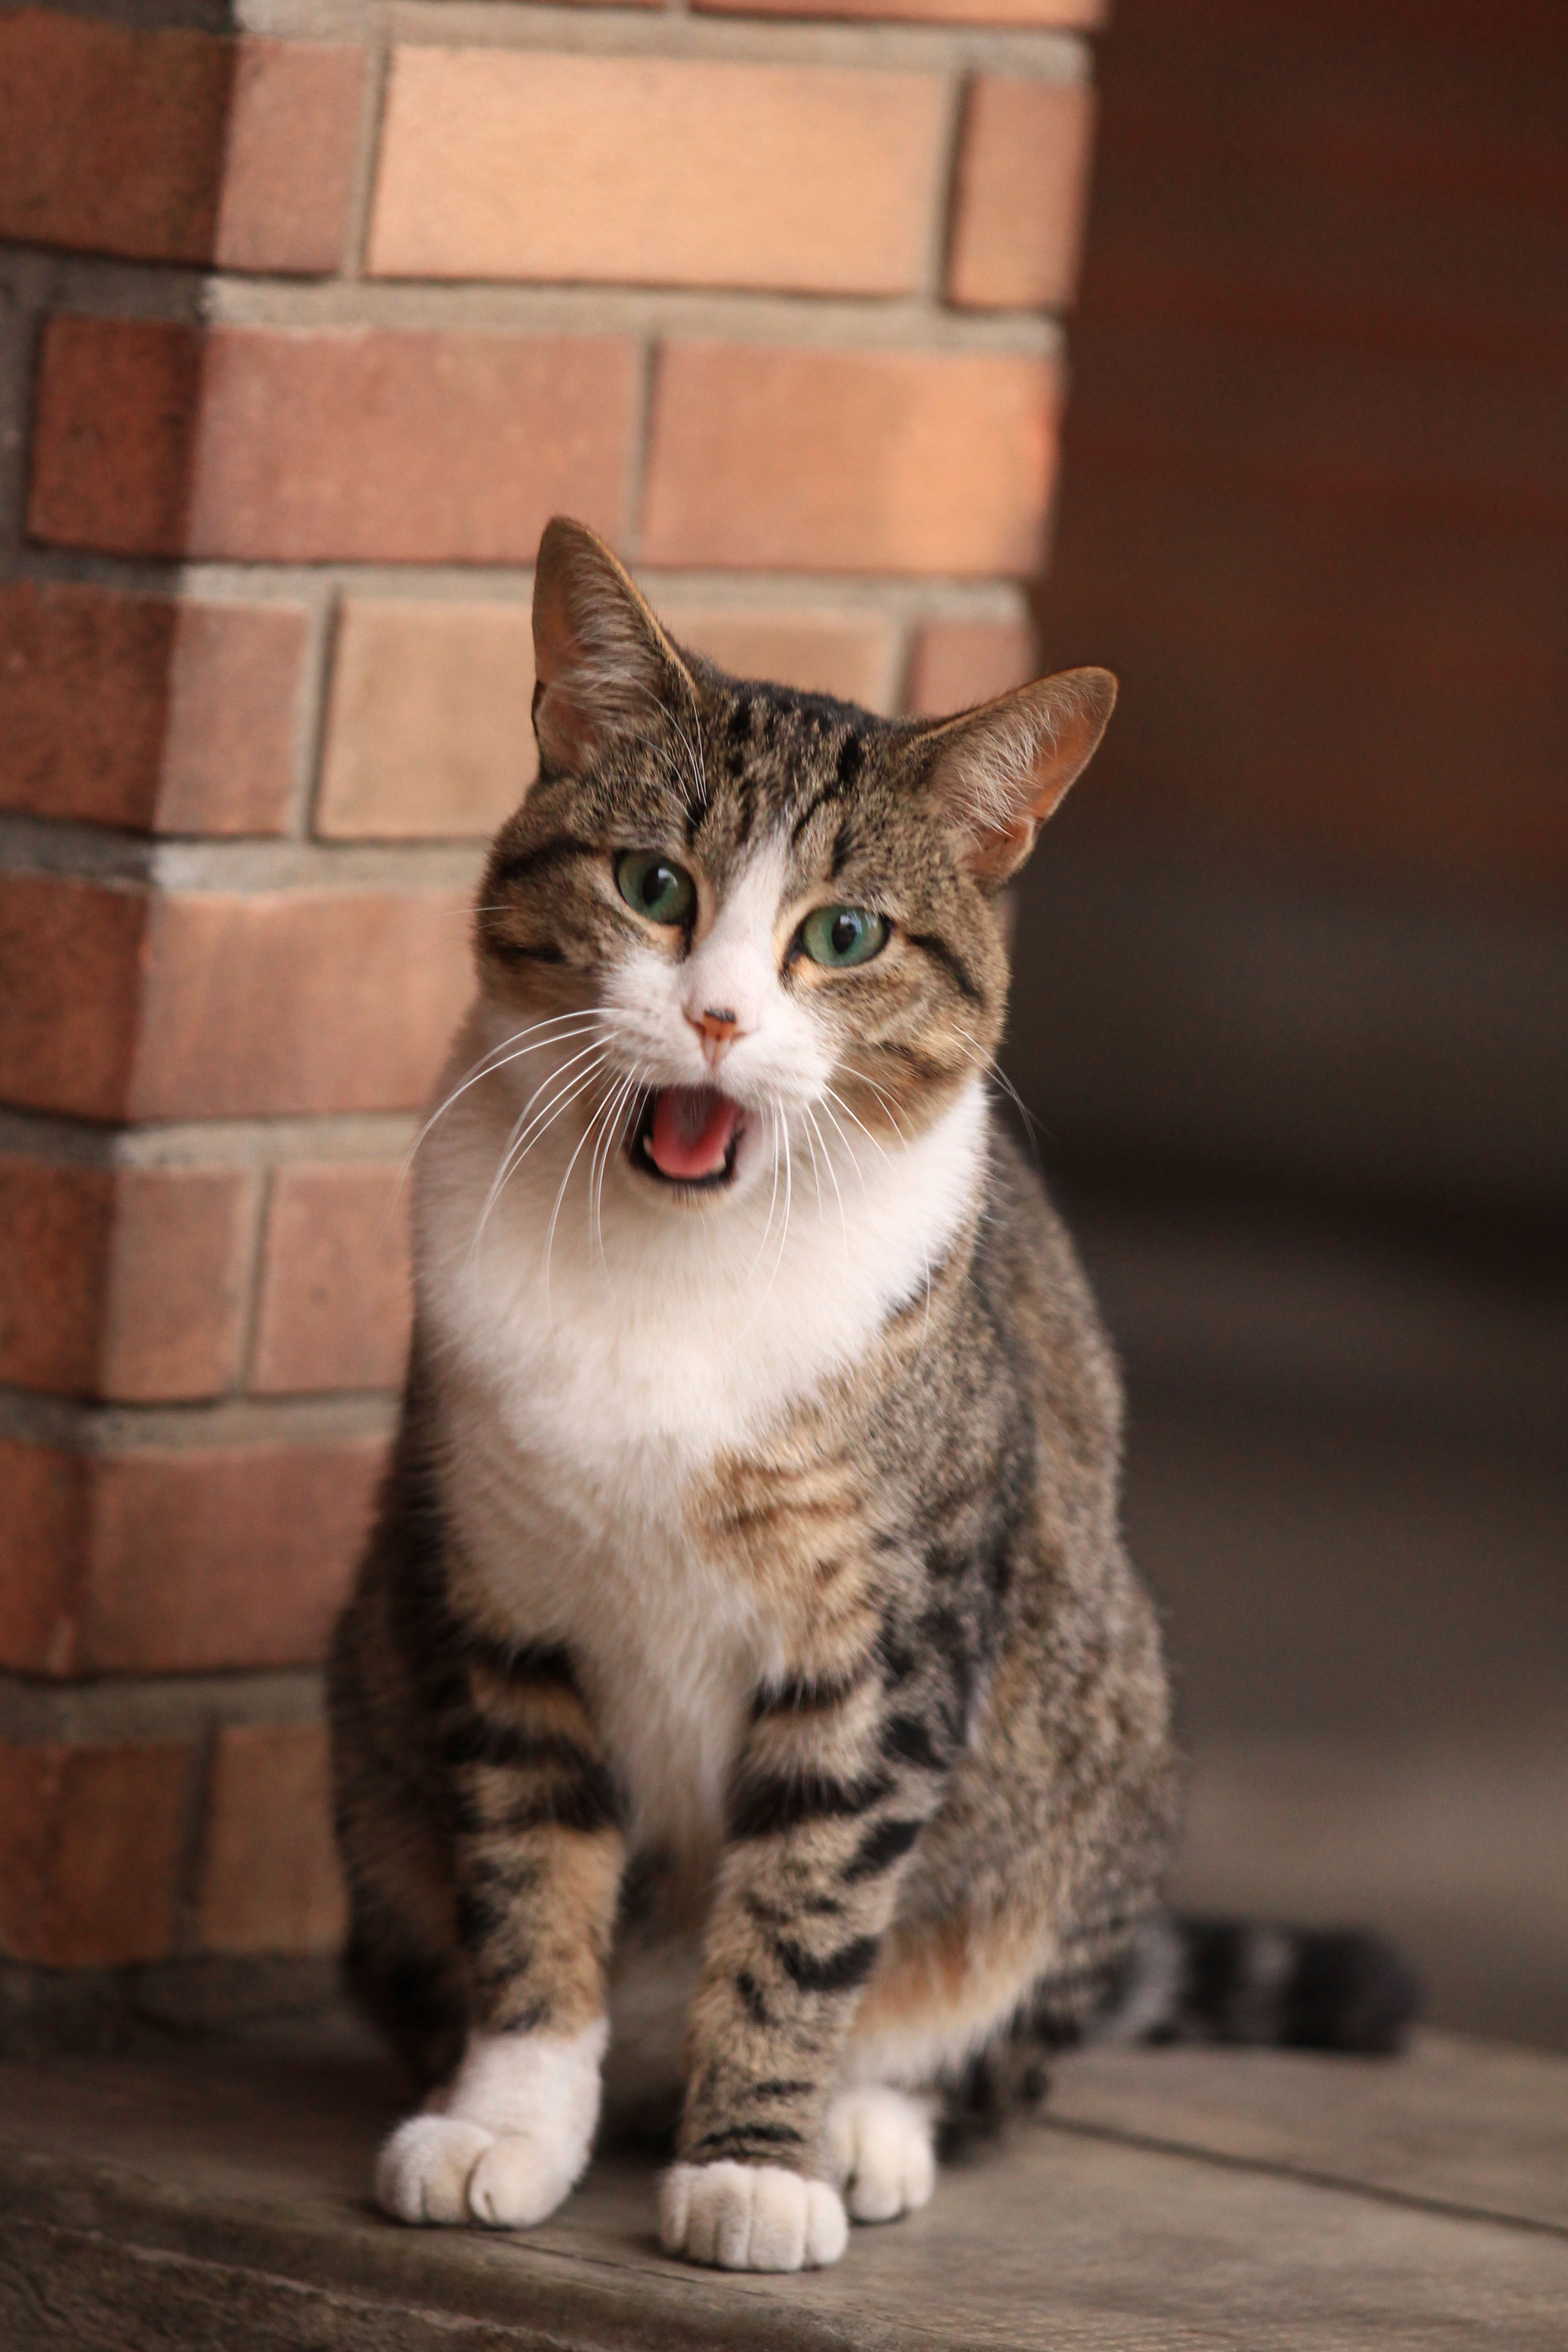
\includegraphics[width=0.3\textwidth]{./Bilder/European_cat_02_16_mp.jpg}
\caption{Picture used for the experiments \cite{cat}}
\label{fig:cat}
\end{figure}
\paragraph{Batch Size}
%%mathe defs of throughput?
Batch Size denotes the number of images fed into the deep learning model in a single inference operation. 
Feeding more than one image to the network can lead to a higher throughput, if enough computational power is available. This increase in throughput often comes at the cost of increased latency and general resource consumption.

To study these trade-offs we conduct experiments with the following batch sizes: 1, 2, 16, 32. Since at the point of these experiments a batch size greater than one is not supported for the TensorFlow Lite versions of MobilenetV2 (both float and quantized), measurements with these batch sizes cannot be performed for the case of edge inference at this point.
\paragraph{NNAPI}
The Android Neural Network API (NNAPI), presented in section \ref{chap:NNAPI}, is supposed to enhance the inference performance of TensorFlow Lite. Therefore we take a look into the effect of this framework.
%%Mention GPU use here
\paragraph{GPU Usage}
Since January 16 an experimental release of TensorFlow Lite supporting GPU usage on Android using OpenGL ES 3.1 Compute Shaders \cite{tfLiteGPU}.
So far only four public models and their operators are supported, including MobileNetV2, but not InceptionV4. 
Therefore we omit the test of this new feature in our experimentation, but our initial testing indicated that the use of NNAPI provides faster inference latencies for MobileNetV2 than the GPU version.
%%https://medium.com/tensorflow/tensorflow-lite-now-faster-with-mobile-gpus-developer-preview-e15797e6dee7
%experimental
%only mobilenet supported
%worse performance than NNAPI so far


\begin{figure}[H]
\centering
 \scalebox{.7}{%\documentclass[border=10pt]{standalone}
%\usepackage{tikz}
%\begin{document}
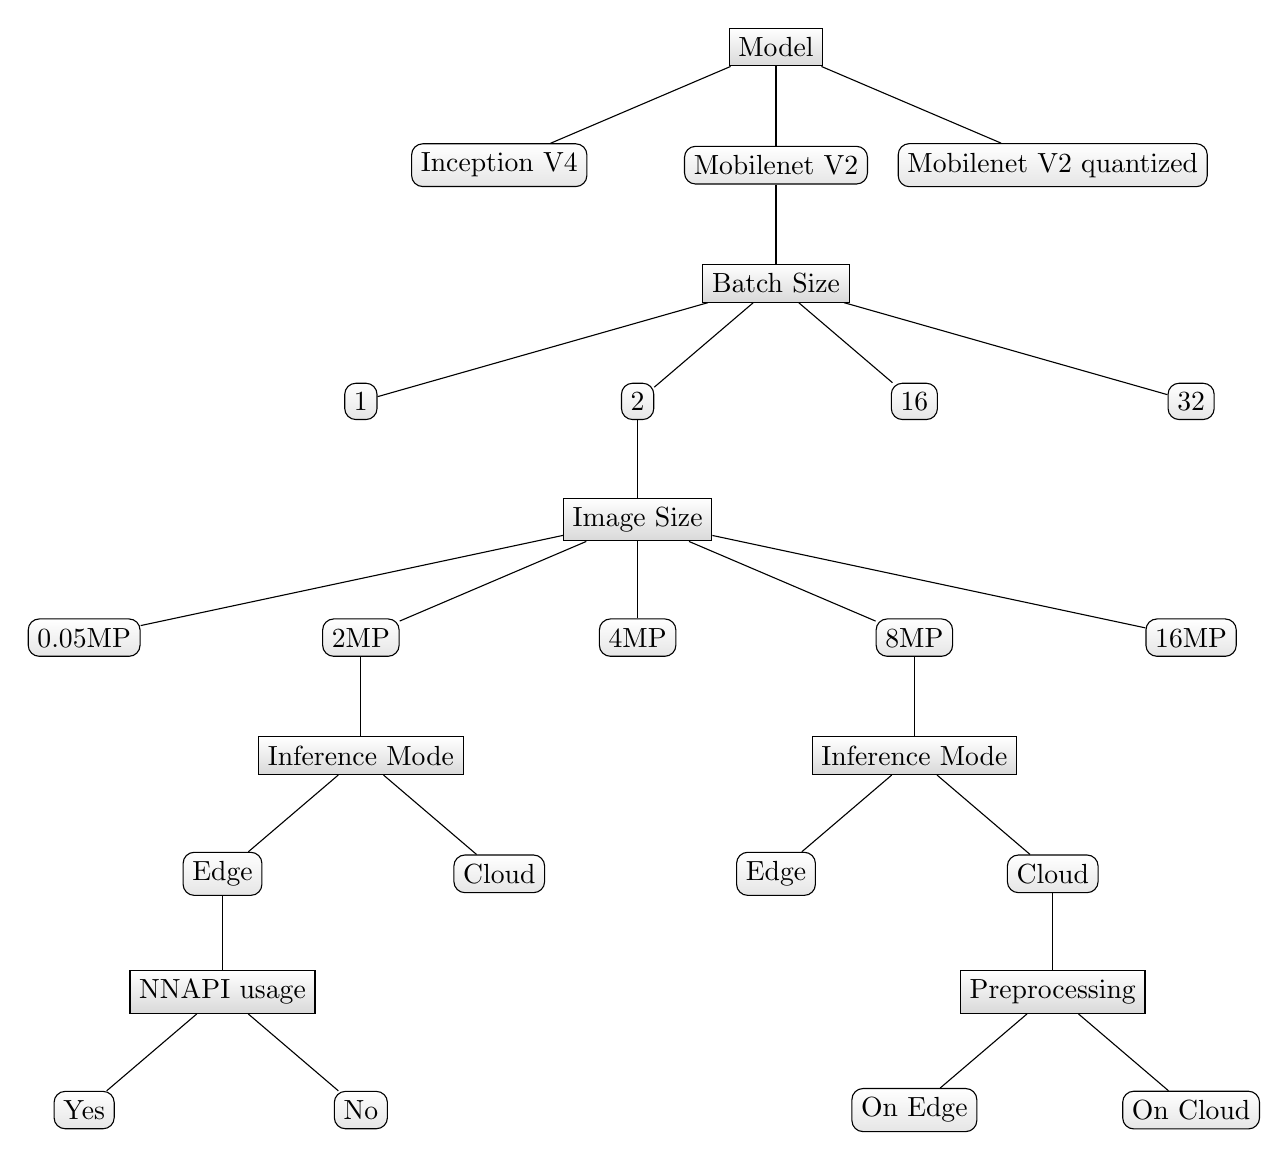
\begin{tikzpicture}[sibling distance=10em,
  param/.style={shape=rectangle,
    draw, align=center,
    top color=white, bottom color=gray!30},
  conf/.style={shape=rectangle, rounded corners,
    draw, align=center,
    top color=white, bottom color=gray!20}  ]  ]
    
  \node[param] {Model}
    child { node [conf]{Inception V4} }
    child { node [conf]{Mobilenet V2}
      child { node [param]{Batch Size}
        child { node [conf]{1} }
        child { node [conf]{2} 
            child { node [param]{Image Size}
                child { node [conf]{0.05MP}}
                child { node [conf]{2MP}
                child { node [param]{Inference Mode}
                        child { node[conf] {Edge}
                            child { node[param] {NNAPI usage}
                                 child { node[conf] {Yes}}
                                 child { node [conf]{No}}}}
                        child { node [conf]{Cloud}
                            }}}
                child { node [conf]{4MP}
                    }
                child { node [conf]{8MP}
                child { node [param]{Inference Mode}
                        child { node[conf] {Edge}}
                        child { node [conf]{Cloud}
                            child { node [param]{Preprocessing}
                               child { node [conf]{On Edge}}
                                child { node [conf]{On Cloud}}}}}}
                child { node [conf]{16MP}}}}
        child { node[conf] {16} }
        child { node [conf]{32} }} }
    child { node [conf]{Mobilenet V2 quantized} };
\end{tikzpicture}
%\end{document}}

\caption{Excerpt of the performed experiments configurations}
\label{fig:tree}
\end{figure}
Figure \ref{fig:tree} shows a part of our experimentation tree. In theory there would be 240 different parameter configurations, but due to a number of reasons the number of different configurations reduced to 113 in total.

First, the Usage of NNAPI is independent of the image size hence we only perform experiments without NNAPI for a single image size. Also the usage of NNAPI leads to a way better performance for edge inference and we want to compare edge and cloud inference, so we only carry out experiments without NNAPI for a batch size of one.
We omit the cloud inference for the quantized MobileNetV2 because the model is so small the network overhead would be overwhelming.%INSERT REASON.

%of limited capacity/time and
Lastly due to lack of support certain operations in TensorFlow Lite for the MobileNetV2 models, we can not perform inference experiment for MobileNetV2 with a batch size larger than one.
\subsection{Performance Metrics}
\label{chap:insta_measurements}
In the following section we describe how we measure the performance metrics defined in \ref{chap:metrics}.
We conduct the measurements either directly in the source code or by using Android Studio Profiler (Version 3.3). Since Android Studio cannot collect all metrics the way we wanted, we wanted to used Trepn as a secondary profiling application. But since Trepn does not support our test device, we had to omit these metrics.

In the following definitions $t_{start}$ denotes the starting point of either the preprocessing or inference, while $t_{end}$ denotes the end point of the respective process.
\subsubsection{Latency}
We measure $Latency_{preprocessing}$ by measuring the time difference between start and end of the preprocessing process.
Note that all latency measurements are reported in milliseconds(ms).
\begin{equation*}
\begin{gathered}
Latency_{preprocessing} = t_{endPreprocessing} - t_{startPreprocessing}
\end{gathered}
\end{equation*}
To measure inference latency we need to distinguish between edge and cloud inference, since for the latter the network latency needs to be considered.

\paragraph{Edge Inference}To measure edge inference latency we measure the time the TensorFlow Lite interpreter needs to run the inference operation on the loaded model given the input image.
\begin{equation*}
\begin{gathered}
Latency_{inference} = t_{endInference} - t_{startInference}
\end{gathered}
\end{equation*}
\paragraph{Cloud Inference}
To measure the cloud inference latency we need to measure two latencies, which combined yield $Latency_{inference}$. The first latency is  $Latency_{server}$. This server latency describes the time difference between the point where TensorFlow Serving receives the inference request and the point in time where TensorFlow Serving sends the response back to the client.
The second latency $Latency_{network}$ denotes the time the prediction request needs to reach the cloud-backend.
These latencies are illustrated in figure \ref{fig:serverLat}.
\begin{figure}[!htb]
\centering


\tikzset{every picture/.style={line width=0.75pt}} %set default line width to 0.75pt        

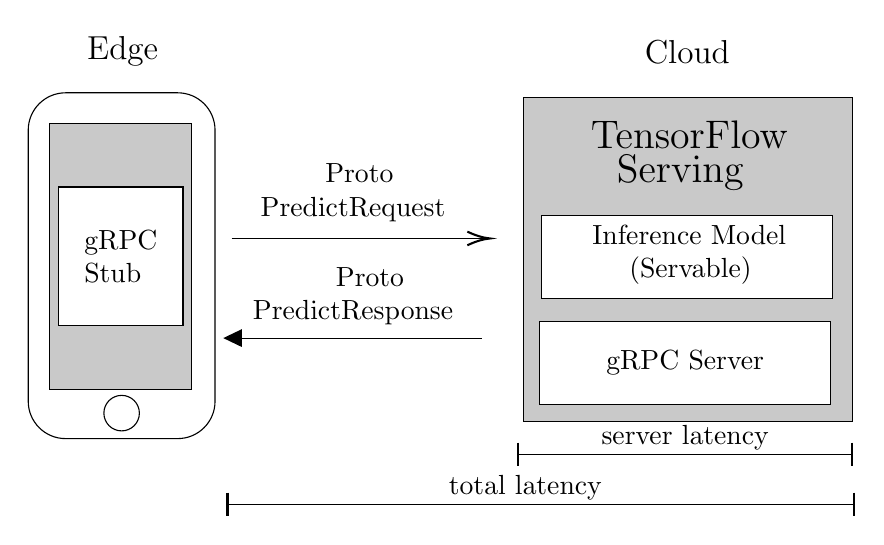
\begin{tikzpicture}[x=0.75pt,y=0.75pt,yscale=-1,xscale=1]
%uncomment if require: \path (0,300); %set diagram left start at 0, and has height of 300

%Straight Lines [id:da7072764839644827] 
\draw    (149.5,277) -- (451.5,277) ;
\draw [shift={(451.5,277)}, rotate = 180] [color={rgb, 255:red, 0; green, 0; blue, 0 }  ][line width=0.75]    (0,5.59) -- (0,-5.59)   ;
\draw [shift={(149.5,277)}, rotate = 180] [color={rgb, 255:red, 0; green, 0; blue, 0 }  ][line width=0.75]    (0,5.59) -- (0,-5.59)   ;
%Straight Lines [id:da9536138531960994] 
\draw    (289.5,253) -- (450.5,253) ;
\draw [shift={(450.5,253)}, rotate = 180] [color={rgb, 255:red, 0; green, 0; blue, 0 }  ][line width=0.75]    (0,5.59) -- (0,-5.59)   ;
\draw [shift={(289.5,253)}, rotate = 180] [color={rgb, 255:red, 0; green, 0; blue, 0 }  ][line width=0.75]    (0,5.59) -- (0,-5.59)   ;
%Shape: Rectangle [id:dp8902536871651789] 
\draw  [fill={rgb, 255:red, 201; green, 201; blue, 201 }  ,fill opacity=1 ] (63.91,93.69) -- (132.34,93.69) -- (132.34,221.63) -- (63.91,221.63) -- cycle ;
%Rounded Rect [id:dp41557214204551274] 
\draw   (53.5,96.82) .. controls (53.5,86.88) and (61.56,78.82) .. (71.5,78.82) -- (125.5,78.82) .. controls (135.44,78.82) and (143.5,86.88) .. (143.5,96.82) -- (143.5,227.43) .. controls (143.5,237.37) and (135.44,245.43) .. (125.5,245.43) -- (71.5,245.43) .. controls (61.56,245.43) and (53.5,237.37) .. (53.5,227.43) -- cycle ;
%Shape: Ellipse [id:dp8878397246816687] 
\draw   (89.95,233.16) .. controls (89.95,228.43) and (93.78,224.6) .. (98.5,224.6) .. controls (103.22,224.6) and (107.05,228.43) .. (107.05,233.16) .. controls (107.05,237.88) and (103.22,241.71) .. (98.5,241.71) .. controls (93.78,241.71) and (89.95,237.88) .. (89.95,233.16) -- cycle ;
%Straight Lines [id:da5813802620369573] 
\draw    (151.48,149) -- (274,149) ;
\draw [shift={(276,149)}, rotate = 540] [color={rgb, 255:red, 0; green, 0; blue, 0 }  ][line width=0.75]    (10.93,-3.29) .. controls (6.95,-1.4) and (3.31,-0.3) .. (0,0) .. controls (3.31,0.3) and (6.95,1.4) .. (10.93,3.29)   ;

%Straight Lines [id:da16220168680973557] 
\draw    (149.48,197) -- (272,197) ;

\draw [shift={(147.48,197)}, rotate = 360] [fill={rgb, 255:red, 0; green, 0; blue, 0 }  ][line width=0.75]  [draw opacity=0] (8.93,-4.29) -- (0,0) -- (8.93,4.29) -- cycle    ;
%Shape: Rectangle [id:dp8411150472244695] 
\draw  [fill={rgb, 255:red, 201; green, 201; blue, 201 }  ,fill opacity=1 ] (292,81) -- (450.5,81) -- (450.5,237) -- (292,237) -- cycle ;
%Shape: Rectangle [id:dp13557861576626729] 
\draw  [fill={rgb, 255:red, 255; green, 255; blue, 255 }  ,fill opacity=1 ] (301,138) -- (441,138) -- (441,178) -- (301,178) -- cycle ;
%Shape: Rectangle [id:dp5681963435258506] 
\draw  [fill={rgb, 255:red, 255; green, 255; blue, 255 }  ,fill opacity=1 ] (68.19,124.22) -- (128.07,124.22) -- (128.07,191.1) -- (68.19,191.1) -- cycle ;
%Shape: Rectangle [id:dp7458124222136935] 
\draw  [fill={rgb, 255:red, 255; green, 255; blue, 255 }  ,fill opacity=1 ] (300,189) -- (440,189) -- (440,229) -- (300,229) -- cycle ;

% Text Node
\draw (370,245) node  [align=left] {server latency};
% Text Node
\draw (293,269) node  [align=left] {total latency};
% Text Node
\draw (210,127) node  [align=left] { \ \ \ \ \ \ \ Proto\\PredictRequest};
% Text Node
\draw (99,59) node  [align=left] {{\large Edge}};
% Text Node
\draw (371,59) node  [align=left] {{\large Cloud}};
% Text Node
\draw (372,109) node  [align=left] {{\Large TensorFlow}\\{\Large  \ \ Serving}};
% Text Node
\draw (372,157) node  [align=left] {Inference Model\\ \ \ \ \ (Servable)};
% Text Node
\draw (210,177) node  [align=left] { \ \ \ \ \ \ \ \ \ Proto\\PredictResponse};
% Text Node
\draw (98.13,157.66) node  [align=left] {gRPC\\ Stub};
% Text Node
\draw (370,209) node  [align=left] {gRPC Server};


\end{tikzpicture}
\caption{Measurement of $Latency_{server}$ and $Latency_{network}$ for Cloud Inference}
\label{fig:serverLat}
\end{figure}


Similar to the edge inference, $Latency_{inference}$ is being measured by calculating the time difference between starting the inference process and receiving the prediction for the given inference request. This whole process is covered by the \emph{predict} function of TensorFlow Serving. Therefore we measure the wall clock time of this function.

Since TensorFlow Serving does not output the server latency, we needed to tweak the source code of gRPC, which is the underlying protocol of TensorFlow Serving. gRPC already logs this latency, so we adjust the source code to output this latency when a call to TensorFlow Serving is finished, repackage the source code and change to dependencies of TensorFlow Serving pointing to the adjusted packages.

We then calculate $Latency_{network}$ implicitly by subtracting $Latency_{server}$ from $Latency_{inference}$.

\begin{equation*}
\begin{gathered}
Latency_{inference} = t_{endInference} - t_{startInference}\\
Latency_{server}= t_{receive Request} - t_{send Response}\\
Latency_{network} = Latency_{inference} - Latency_{server}
\end{gathered}
\end{equation*}


The total latency $Latency_{total}$ for both edge and cloud inference is simply calculated by summing up the latencies of both preprocessing and inference.
\begin{equation*}
\begin{gathered}
Latency_{total} = Latency_{preprocessing} + Latency_{inference}
\end{gathered}
\end{equation*}
\subsubsection{Energy Consumption}
Since Android Studio Profiler only estimates the energy consumption in the form of low, medium and high, the tool is not fit to provide empiric measurements. The Trepn Power Profiler would provide such measurements, but does not support the device used for the experiments (OnePlus 6T).
\subsubsection{CPU Usage}
We measure the CPU usage(\%) of both preprocessing as the maximum CPU usage during the respective processes.
\begin{equation*}
\begin{gathered}
%%CPU_{preprocessing} = max_{[start_{preprocessing}, end_{preprocessing}]}(CPU)\\
%%CPU_{inference} = max_{[start_{inference}, end_{inference}]}(CPU)\\
CPU_{preprocessing} = \max\limits_{t_{startPreprocessing} \leq t \leq t_{endPreprocessing}} CPU_{Usage}(t)\\
CPU_{inference} = \max\limits_{t_{startInference} \leq t \leq t_{endInference}} CPU_{Usage}(t)
\end{gathered}
\end{equation*}
Android Studios’ CPU Profiler allows us to record the maximum CPU usage for both preprocessing and inference. To minimize the impact on the Android Profiler on the performance of the application we disable allocation tracking.
\begin{figure}[H]
\centering  
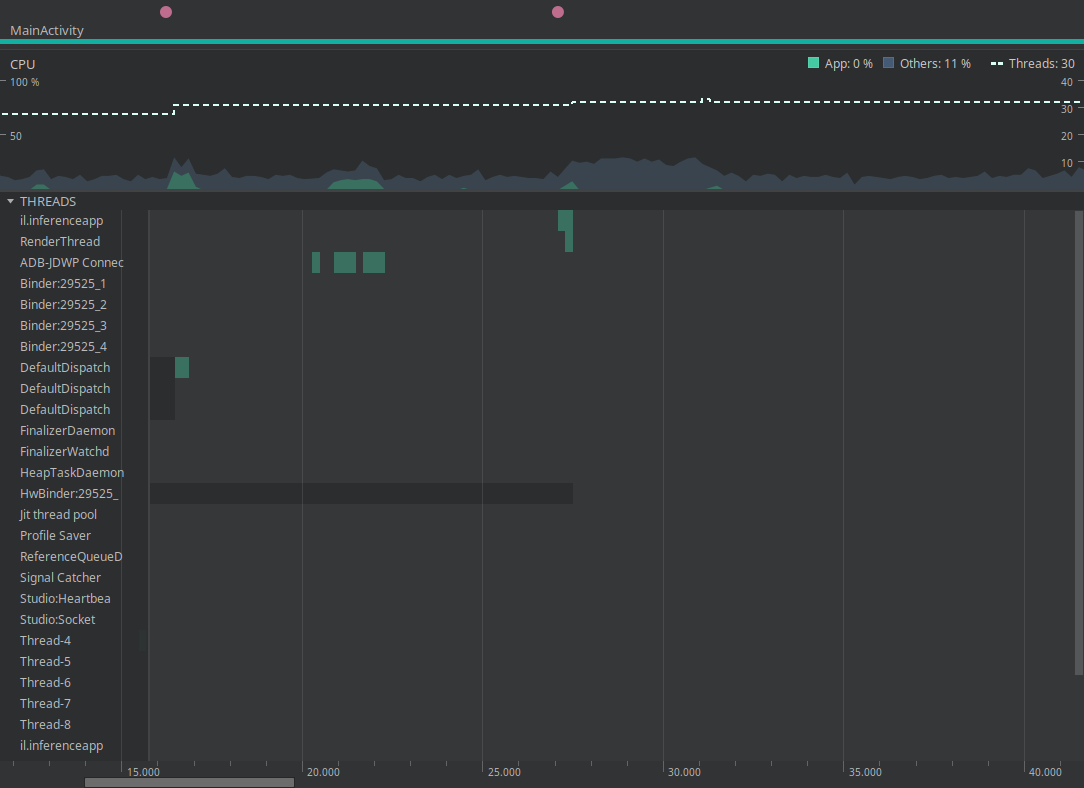
\includegraphics[width=0.6\textwidth]{./Bilder/profiler_CPU}
\caption{Android CPU Profiler}
\label{fig:prof_cpu}
\end{figure}
\subsubsection{Memory Usage}
We measure the memory usage by recording the maximum memory consumption during both processing and inference. Both of the following metrics are reported in megabytes(MB) in the result section.
\begin{equation*}
\begin{gathered}
Memory_{preprocessing} = \max\limits_{t_{startPreprocessing} \leq t \leq t_{endPreprocessing}} Memory(t)\\\\
Memory_{inference} = \max\limits_{t_{startInference} \leq t \leq t_{endInference}} Memory(t)\\
\end{gathered}
\end{equation*}
The Memory Profiler is part of Android Studio Profiler and shows the memory consumption of the app it is profiling. Memory allocations by the operating system or other apps are not recorded. Besides recording the total amount of memory allocated the Profiler also tracks the different categories, for example memory allocated by Java/Kotlin code. We always record the maximum consumed memory for each operation.
%%memory not accurate over 1GB
Note that for values greater than $1000$MB the profiler only reports gigabyte values with one decimal place. For example the profiler reports $1410$MB as $1.4$GB.

Figure \ref{fig:prof_mem} depicts an example of the Memory Profiler for a single experiment. The first peak in memory consumption is the preprocessing step, while the second peak is caused by the inference process.
The little trash can at the bottom of the figure shows that the garbage collection was called. The garbage collection was always manually called after the preprocessing in case not all unneeded memory allocations are collected before running the inference operation. 
Note that we report total memory consumption of the application, including memory consumed for the graphical interface or the \emph{Logger} class.
%In the case of preprocessing only the preprocessed image is needed, so the 
\begin{figure}[H]
\centering
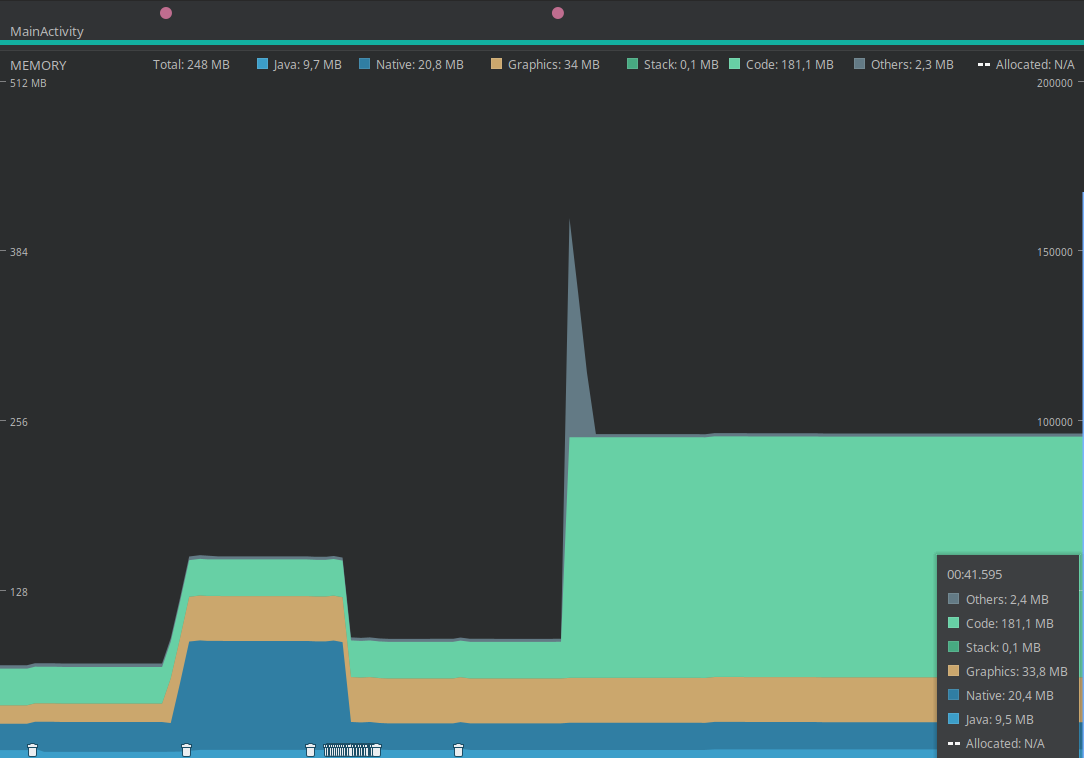
\includegraphics[width=0.6\textwidth]{./Bilder/profiler_MEM}
\caption{Android Memory Profiler}
\label{fig:prof_mem}
\end{figure}
\subsubsection{GPU Usage}
Neither Android Studio nor Trepn can provide GPU metrics for the OnePlus 6T. Hence no GPU measurements can be conducted.
\subsubsection{Throughput}
We differentiate three types of throughput: the inference throughput, preprocessing throughput and the total throughput, which also includes preprocessing besides inference.
We calculate throughput in operations per second by 

\begin{equation*}
\begin{gathered}
Throughput_{preprocessing} =\frac{1000}{(Latency_{preprocessing}) / batchsize}\\
Throughput_{inference} =\frac{1000}{(Latency_{inference}) / batchsize}\\
Throughput_{total}  =\frac{1000}{(Latency_{total}) / batchsize}
\end{gathered}
\end{equation*}
\subsubsection{Data Consumption}
We measure both transmitted and received data by using the Android TrafficStats package (https://developer.android.com/reference/android/net/TrafficStats). We start measuring both transmitted and received bytes when the inference operation is started and stop when the response from the server is returned. We report both $Data_{transmitted}$ and $Data_{received}$ in kilobytes(KB).
\begin{equation*}
\begin{gathered}
Data_{transmitted} = \sum_{t_{startInference}}^{t_{endInference}} Data_{transmitted}(t)\\
Data_{received} = \sum_{t_{startInference}}^{t_{endInference}} Data_{received}(t)
\end{gathered}
\end{equation*}
\section{Results and Evaluation}
The previous section covered the experimental design, including used models, hardware devices and framework, as well as definition of performance metrics. Using this design specifications, we will now present and evaluate the results of the conducted experiments.

First, we take a look into the individual results of edge and cloud inference and afterwards compare them against each other. In each of these sections first the preprocessing and then the inference results are presented. 
In the last subsection we take a seperate look at batch sizes larger than one.

%die 83mb aufschlüsseln in GUI etc 
%Logger verbrauch erwähnen
Note that the Android application consumed around 83MB in memory and 0\% CPU during idle. Additionally the logger, which is used to save the measurements of the experiments consumes memory as well, hence the memory consumption shown in the results include both logger and other memory overhead caused by the graphical interface etc.

For precise mean values and standard deviations of all measured metrics refer to tables \ref{measurementsInception} and \ref{measurementsMobilenet}.

The black bar on top of each bar of the following bar chart and translucent areas around the lines of the line plots represent the standard deviation.

Preprocessing is performed without any models loaded on the edge. but with the image loaded into memory before the start of preprocessing to prevent the I/O operations to influence the preprocessing performance.
Edge Inference is done using a loaded model. We do not consider model loading latency in this thesis.

All experiments are done using the eduroam Wi‑Fi, since the cloud-backend server hosted at the LRZ is only reachable within the Münchner Wissenschaftsnetz (MWN) and a VPN would have an impact on network latencies.

We conducted the experiments in multiple sessions, where each session consists of $100$ experiments distributed over about two hours, thus preventing the results to be skewed by thermal throttling.
\subsection{Edge Inference}
This section covers the results of the edge inference experiments with OnePlus 6T device presented in section \ref{chap:hardwareEdge}.

Note that this section only covers the results for a batch size of one, for the results of larger batch sizes please refer to section \ref{chap:resultsBatchSize}.

\FloatBarrier
\subsubsection{Preprocessing}
\label{chap:edgePrepro}
Figure \ref{fig:EdgePrepro} shows the $Latency_{preprocessing}$ and $Memory_{preprocessing}$ for the different image sizes and models.

There is little difference in both latency and memory for the different models. 
InceptionV4 uses on average $7.5$MB more memory (or $5\%$) than the MobileNetV2 models, which is caused by the models higher input size (InceptionV4 $299\times299$, MobileNetV2 $224\times224$). 
These small differences are expected, since both all three model require roughly the same input specifications, with the exception of input size, but the difference between the two input sizes is relatively small.

While the different models have little difference in memory and latency, the image size has an significant impact on both of these metrics.
A $16$ megapixel image takes on average across all models more than $10$ times as long to preprocess as well as using $1.5$ times more memory in comparison to a $224^2/299^2$ image.
Figure \ref{fig:EdgePrepro} shows a steady increase of $Latency_{preprocessing}$ and $Memory_{preprocessing}$ across the increasing image sizes.
Preprocessing of large images is therefore mainly affected by the resizing process, not the pixel normalization or conversion to a \emph{ByteBuffer}, since these steps are performed after the resizing, thus having the same impact on performance as they would have on an $224^2/299^2$ image.

The standard deviation of both memory and latency are both low, indicating a stable resource consumption.


%%factors reinbringen auch kb größe der bilder
%%mehr impact on latency than memory

\begin{figure}[!htb]
\centering
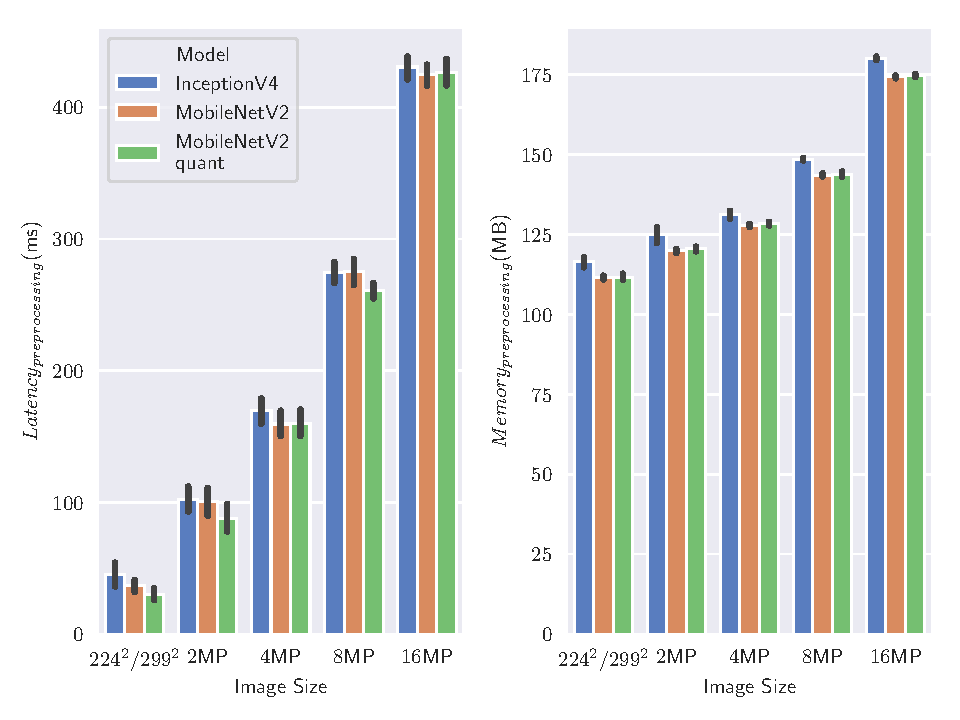
\includegraphics[width=0.8\textwidth]{./Bilder/single_plots/edge_inference_plots/Edge_Inference_Preprocessing.pdf}
\caption[Edge Inference - Preprocessing $Latency_{preprocessing}$, $Memory_{preprocessing}$]{Edge Inference - Preprocessing $Latency_{preprocessing}$, $Memory_{preprocessing}$ -  lower is better: Increasing image sizes have increasing impact on both memory and latency, independent of model type}
\label{fig:EdgePrepro}
\end{figure}
%%Was über CPU hier sagen
%%CPU usage in obere grafik integrieren?
Looking the CPU usages during preprocessing (see figure \ref{fig:CloudEdgePreproCPU}) one can see that the usages are very similar across all models and image sizes. This is probably due to the fact that the preprocessing of a single image is done on a single core. Since the OnePlus 6T has $8$ cores, the maximal CPU usage cause by a single core is $12.5\%$, which also is displayed in the plot, where all usages are close to this number.
%%High variance
%%around?

\FloatBarrier
\subsubsection{Inference}
This section presents the results for edge inference, in particular the effect of the Android Neural Network API.
Different image sizes have no effect on edge inference, as image are always preprocessed when they reach the inference step.
Hence we do not consider the different image sizes in the majority of this section.


\begin{comment}
\begin{figure}[H]
\centering
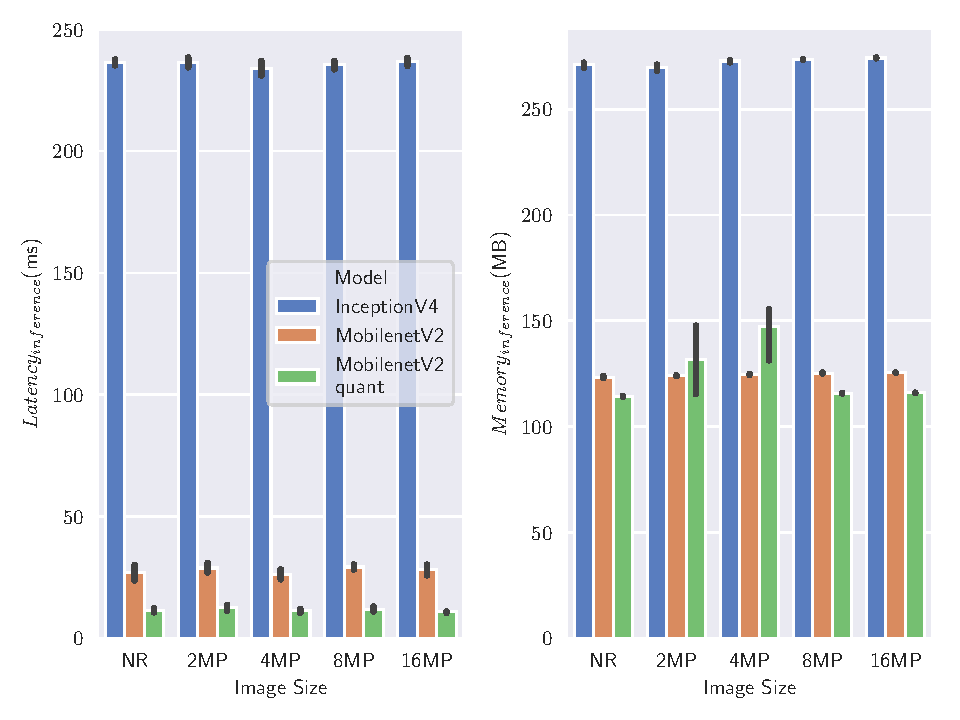
\includegraphics[width=0.8\textwidth]{./Bilder/single_plots/edge_inference_plots/Edge_Inference_Inference.pdf}
\caption{Edge Inference - Inference}
\label{fig:EdgeInference}
\end{figure}


\end{comment}
\subsubsection{Effect of NNAPI}
%%effcient
The Android Neural Network API (NNAPI) is supposed to speed up inference of neural network on Android by introducing optimised kernels/operators. 
The effect of this framework can be seen in figure \ref{fig:NNAPI} and show the significant performance improvement caused by the NNAPI, not only affecting $Latency_{inference}$, but also $Memory_{inference}$ and $CPU_{inference}$.

%%Genauere factors einfügen : inferecen zweimal so schnell...
This effect can be observed across all tested models, but especially on the InceptionV4 network.

Note that the NNAPI uses the GPU of the OnePlus 6T for a part of its inference, therefore while reducing the CPU usage during inference, the NNAPI probably causes higher GPU usages.

Since the NNAPI leads to performance improvements in all measured metrics, it will be used for all further edge inference results.

\begin{figure}[!htb]
\centering
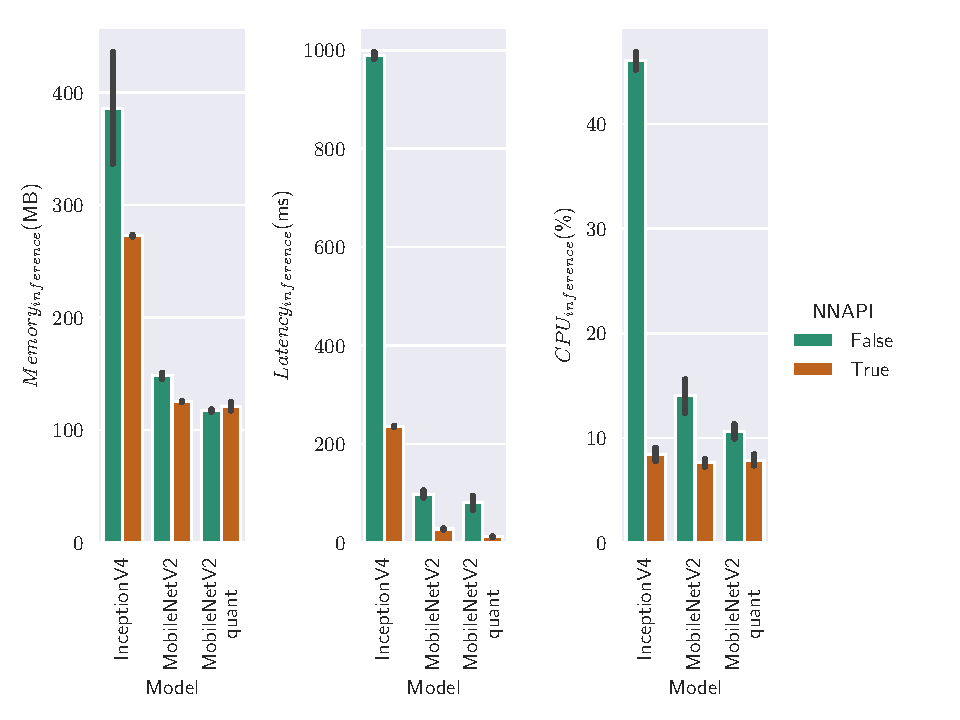
\includegraphics[width=0.9\textwidth]{./Bilder/single_plots/edge_inference_plots/NNAPI_behavior.pdf}
\caption[Edge Inference - Effect of NNAPI on Inference]{Edge Inference - Effect of NNAPI on Inference - lower is better: NNAPI has a significant positive effect on the inference metrics latency, memory and CPU usage.}
\label{fig:NNAPI}
\end{figure}

%, InceptionV4, MobileNetV2 and the quantized version of MobileNetV2,
When comparing the different models with NNAPI enabled it can be stated that there a significant performance differences between these models.
%%MobileNet und Inception vergleichen
%begründen: effect of quant mit paper vergleichen
%unterschiede mobileNet inception vergleichen
%%danahc MobileNet mit quantized
On average, InceptionV4 inference causes higher inference latencies of factor $8$ and consumes twice as much memory as MobileNetV2.
This contrast in performance is as expected, since MobileNetV2 architecture only contains $8\%$ of InceptionV4's parameter number (see table \ref{table:modelOverview}).
This bigger architecture as well as bigger input size lead to higher memory demands and latencies, thus explaining the performance differences.

A similar difference in inference latency can be seen when comparing MobileNetV2 against its quantized version, where the quantized version is more than $2$ times faster, confirming the study results of \cite{Quantizing} presented in section \ref{chap:quant}.
While there is a difference in latency between the quantized and non quantized versions of MobileNetV2, there is nearly no discrepancy in memory consumption.



While having big impact on both latency and memory, the different models have 
negligible CPU usage differences, but probably not on GPU usage, which we can not report in this thesis.




%%%%%%%%%%%%%%%%%%%%%%%%%%%%%%%%%%%%%%%%%%%%%%%%%%%%%%%%%%%%%%%%%%%
%%%%%Edge Inference Prepro Vs Inference%%%%%%%%%%%%%%%%%%%%%%%%%%%%%%%%%%

Figure \ref{fig:EdgeInferenceRatio} depicts the latency ratio between preprocessing and inference.
As image sizes increases, the preprocessing becomes more and more the bottleneck, especially for the MobileNetV2 models.
For the MobileNetV2 even $224\times224$ images take longer to preprocess than to perform the inference on them.
%The Inception models are far more computational intensive, hence the longer inference latencies, but still 
\begin{figure}[!htb]
\centering
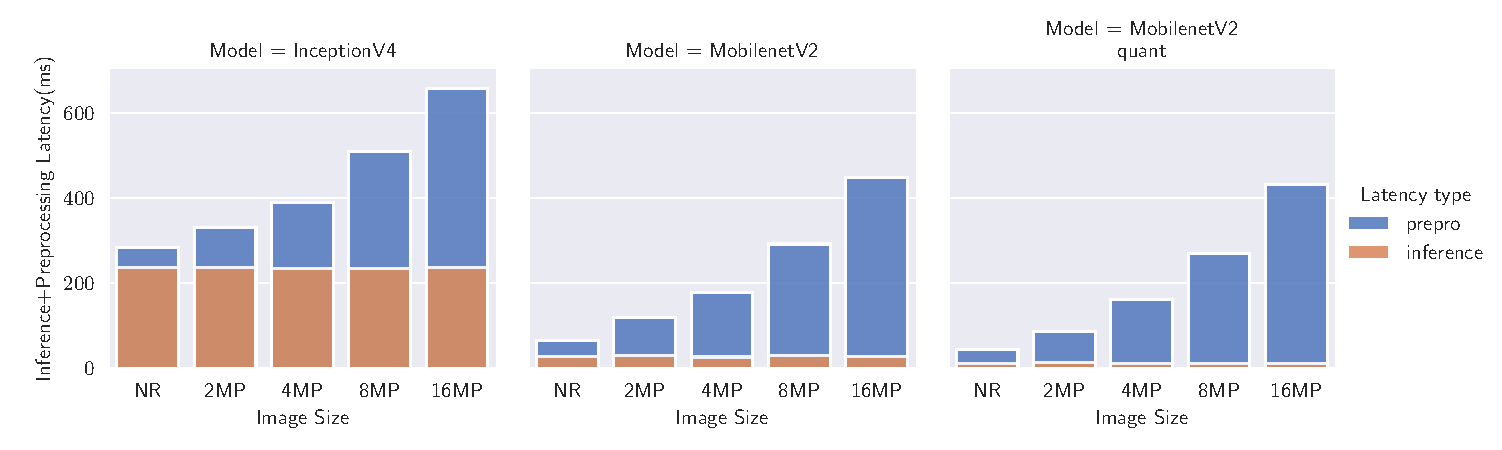
\includegraphics[width=0.95\textwidth]{./Bilder/single_plots/edge_inference_plots/Edge_Preprocessing_+_Inference.pdf}
\caption[Edge Inference - Ratio of Preprocessing and Inference in $Latency_{total}$]{Edge Inference - Ratio of Preprocessing and Inference in $Latency_{total}$ - lower is better: Preprocessing becomes the decisive factor for $Latency_{total}$ of both models for larger image sizes.}
\label{fig:EdgeInferenceRatio}
\end{figure}


\paragraph{Edge Inference - Key Takeaways}
\emph{
\begin{itemize}
    \item Preprocessing becomes bottleneck for larger image sizes.\\
          $16$ MP image in comparison to a $224^2/299^2$ image needs
    \begin{itemize}
        \item $10\times$ slower $Latency_{preprocessing}$
        \item $1.5\times$ more $Memory_{preprocessing}$
    \end{itemize}
    \item NNAPI leads to way better performance across all models:
    \begin{itemize}
        \item $4\times$ faster $Latency_{inference}$
        \item $1.2\times$ less $Memory_{inference}$
        \item $3\times$ less $CPU_{inference}$
    \end{itemize}
    \item In comparison to InceptionV4 MobileNetV2 leads to:
    \begin{itemize}
        \item $8.6\times$ faster $Latency_{inference}$
        \item $2.2\times$ more $Memory_{inference}$
    \end{itemize}
    \item Quantization of MobileNetV2 results in $2.3$x faster $Latency_{inference}$
    \item Preprocessing affects latency more than inference across all images sizes for small networks.
\end{itemize}}

\FloatBarrier
\subsection{Cloud Inference}
This section deals with the results of the cloud inference experiments and their evaluation, divided into preprocessing and inference.
Note that this section only covers the results for a batch size of one, for the results of larger batch sizes please refer to section \ref{chap:resultsBatchSize}.
We are evaluating $Latency_{inference}$ for the most cloud inference results, thus including the network component $Latency_{network}$, because this factor would also be present in real world AI applications. In our case we have a high speed connection with low network latency, thus being a lower bound for real-time AI applications.
%%add network proof (ping and upload)
\subsubsection{Preprocessing}
Cloud Inference allows two preprocessing methods, either on the edge beforehand or directly on the cloud.
This section present the results of these two methods, especially their impact on the resource consumption of edge devices.

Figures \ref{fig:cloudInferencePreproLat} and \ref{fig:cloudInferencePreproMemory} display the effect of preprocessing on either edge or cloud on the preprocessing latencies and memory consumption on the edge in respect to the different deep learning models and image sizes.

For Edge preprocessing, $Memory_{preprocessing}$ and $Latency_{preprocessing}$ are heavily affected by rising image sizes, but not by the different models and their different image input sizes.
Since preprocessing on the edge is very similar as in the edge inference case, please refer to section \ref{chap:edgePrepro} for full details on the edge preprocessing results.

Preprocessing on the cloud leads to an significant decrease in $Latency_{preprocessing}$, which is expected since nearly no preprocessing steps are done on the edge except building a \emph{PredictRequest} object for TensorFlow Serving.
Preprocessing an $224^2/299^2$ image on the edge instead of the cloud causes $20$ times ($1.9/39.8$ms) higher $Latency_{preprocessing}$ and an increase of factor $11$ ($37.9/431.1$ms) for an $16$MP image.
The impact of larger image sizes on memory in the case of cloud preprocessing is marginal, especially in comparison for the edge preprocessing counterparts. This is expected, since only compressed \emph{PNG} images are loaded into memory, in contrary to edge preprocessing, where in addition to the decoded \emph{PNG} images the resized images are also loaded to memory simultaneously.
While $Memory_{preprocessing}$ is lower for cloud preprocessing, the difference is nowhere as substantial as the latency differences. $16$MP images need $1.3$ times ($137.7/179.6$MB) more memory if preprocessing on the edge instead on the cloud.
%%Mention CPU

\begin{figure}[!htb]
\centering
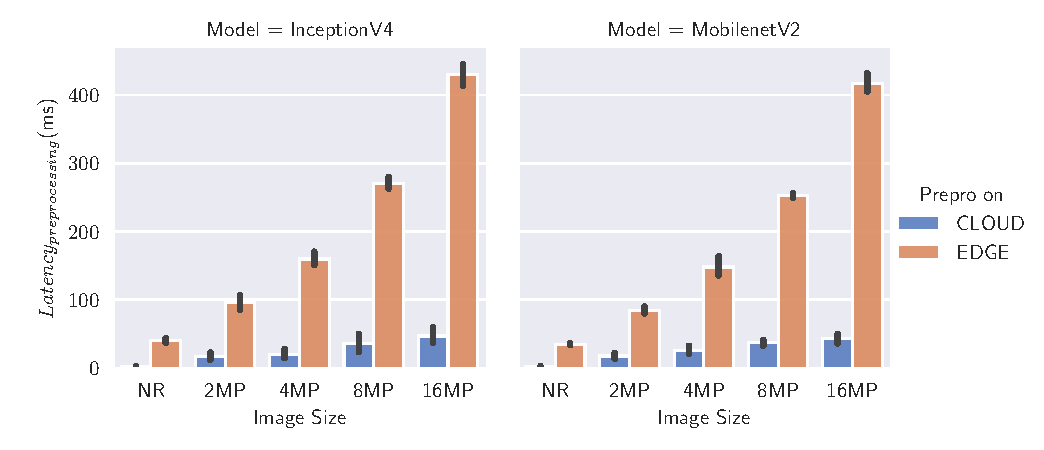
\includegraphics[width=0.95\textwidth]{./Bilder/single_plots/cloud_inference_plots/Cloud_Inference_Preprocessing_Latency.pdf}
\caption{Cloud Inference -  $Latency_{preprocessing}$}
\label{fig:cloudInferencePreproLat}
\end{figure}

\begin{figure}[!htb]
\centering
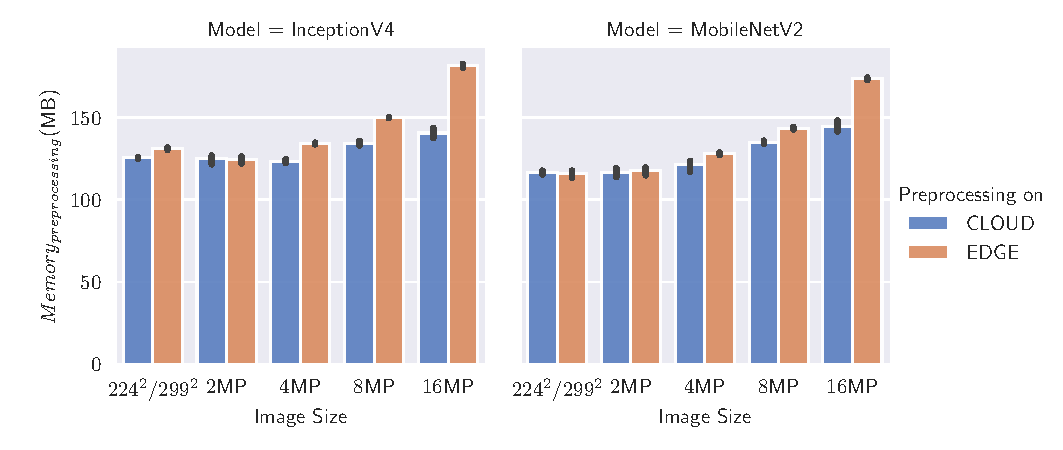
\includegraphics[width=0.95\textwidth]{./Bilder/single_plots/cloud_inference_plots/Cloud_Inference_Preprocessing_Memory.pdf}
\caption{Cloud Inference -  $Memory_{preprocessing}$ - lower is better:}
\label{fig:cloudInferencePreproMemory}
\end{figure}

\FloatBarrier
\subsubsection{Inference}
This section focuses on performance differences between the models and the impact of cloud preprocessing on cloud inference.
The inference metrics for cloud preprocessing include both preprocessing and inference.

%%Also includes preprocessing!!!!

Looking at the memory consumption during inference in figure \ref{fig:cloudInferenceInferenceMemory} one can see that $Memory_{inference}$ is very stable across all image sizes for edge preprocessing, which logical, since all image have been preprocessed to the same shape ($224^2/299^2$), therefore all requests sent to TensorFlow Serving have the same size.
MobileNetV2 uses $10.5$MB less memory on average than InceptionV4, because of its smaller model input size.

For cloud preprocessing the memory consumption increases for increasing image sizes, since larger images are being sent to the server, thus larger images are loaded into the \emph{PredictRequest} object, that is being sent to TensorFlow Serving.
$299^2/224^2$ images consume $123.8/112.34$MB, while $16$MP images $140.1/133.76$, therefore $Memory_{inference}$ increases by $19/13\%$ for InceptionV4/MobileNetV2 respectively.
%%add factor here
There are no $Memory_{inference}$  differences between the two models, since un-preprocessed images are being sent, except for the $224^2/299^2$ images, where the smaller $224^2$ image consumes $7.5$MB less memory on average.
\begin{figure}[!htb]
\centering
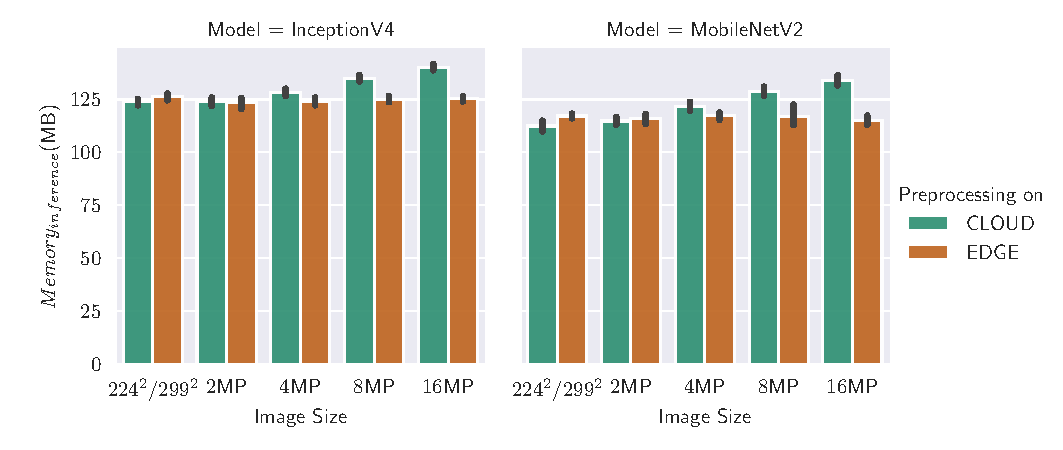
\includegraphics[width=0.95\textwidth]{./Bilder/single_plots/cloud_inference_plots/Cloud_Inference_Memory.pdf}
\caption{Cloud Inference -  $Memory_{inference}$}
\label{fig:cloudInferenceInferenceMemory}
\end{figure}
The $Latency_{inference}$ results can be seen in figure \ref{fig:cloudInferenceInferenceLatency}.
Like for the memory, the latency for edge preprocessing stays the same across all image sizes, since all image sizes are preprocessed on the edge beforehand. 
Mean latencies are $181.2$ms and $108.46$ms for InceptionV4 and MobileNetV2 respectively, therefore MobileNetV2 is $1.7$ times faster.
Figure \ref{fig:CloudInferenceRatioEdgetotal} displays the share of $Latency_{network}$ and $Latency_{server}$ in $Latency_{inference}$ and one can see that the network is accountable for about $20\%$ of the  inference latency for InceptionV4 and $30\%$ for MobileNetV2.

If the images are preprocessed on the cloud, the preprocessing step on the cloud has an significant impact on $Latency_{inference}$, as can be seen in figure \ref{fig:cloudInferenceInferenceLatency}.
While an $224^2/299^2$ image has an latency of $95.8/64.5$ms for InceptionV4/MobileNetV2, a $16$MP image needs $21.9/17.8$ times longer with a $1702.3/1414.8$ms mean latency.
\textbf{This increase applies to all image sizes in a linear proportion.}
Looking at  the share of $Latency_{network}$ in $Latency_{inference}$ in figure \ref{fig:CloudInferenceratioCloudtotal}, the network takes up to $50\%$ of the inference latency for $224^2/299^2$ images, but shrinks to less than $15\%$ for all remaining image sizes.
Therefore it can be stated that the network is not reason for the increase in latency for the larger image sizes, but rather the preprocessing done on the cloud-backend by TensorFlow Serving.
We think Tensorflow's \emph{resize\_bilinear} function, which we use to resize the images, causes the bottleneck in the preprocessing step on the cloud.%%add GPU kernel optimisations issues
%(enter source here)
The use of a other resize approach like nearest-neighbor could speed up preprocessing, but would probably have an impact on the accuracy of the predictions.
While the network connection in our experimentation environment is fast enough too prevent any bottlenecks caused by the network, a slower network connection could slow down inference for large image sizes.
%warum preprocessing s langsam bei tensorflow serving?

%%cloud preprocessing bigger images higher variance
Comparing the two cloud inference options, edge and cloud preprocessing,  $Latency_{inference}$ values for edge preprocessing of both models are faster for all image sizes except the $224^2/299^2$ images.
We believe the $224^2/299^2$ images are faster because of the lower I/O overhead in comparison to the larger preprocessed counter parts, even if the un-preprocessed images still have the decoded and normalized.


This stays also true for $Latency_{total}$ (see figures \ref{fig:CloudInference+PreproCloud} and \ref{fig:CloudInference+PreproEdge}), which includes both $Latency_{preprocessing}$ and $Latency_{inference}$. 
For $224^2/299^2$ images need $223.1/147.2$ms $Latency_{total}$ for InceptionV4/MobileNetV2 for edge preprocessing, while cloud preprocessing needs up $96.9/64.3$ms, therefore cloud preprocessing being $2.3$ times faster.
In contrast cloud inference with edge preprocessing is faster by a factor of $2.7$ for $16$MP images, with the latencies of InceptionV4/MobileNetV2 being $626.7/532$ms for edge preprocessing and $1673.4/1453.9$ms for cloud preprocessing. $2$MP images are $1.7/1.8$ times faster when using edge preprocessing, $4$MP $2.1/2.2$ and $8$MP $2.6/3$ times faster.
%latency edge vs cloud prepro inference:
While MobileNetV2 is $1.75$ times faster in $Latency_{inference}$ for edge preprocessing than InceptionV4, this latency difference shrinks for cloud preprocessing for larger images, started by a difference of factor $1.52$ for $224^2/299^2$ images and shrinking to $1.25/1.21/1.09/1.15$ for the respective image sizes $2/4/8/16$MP.
We believe this decrease is due to the fact as images for MobileNetV2 need to be resized to a smaller input size than InceptionV4, hence increasing the already high resize overhead and thus narrowing the latency difference between both models.
When comparing memory consumption of cloud inference with ether cloud preprocessing or edge preprocessing, the difference is only $3\%$ for  $224^2/299^2$ images ($121.5$MB for edge preprocessing and $118.1$Mb for cloud preprocessing), but $14\%$ for $16$MP images (edge preprocessing $120.0$Mb, cloud preprocessing $136.9$MB).

\begin{figure}[!htb]
\centering
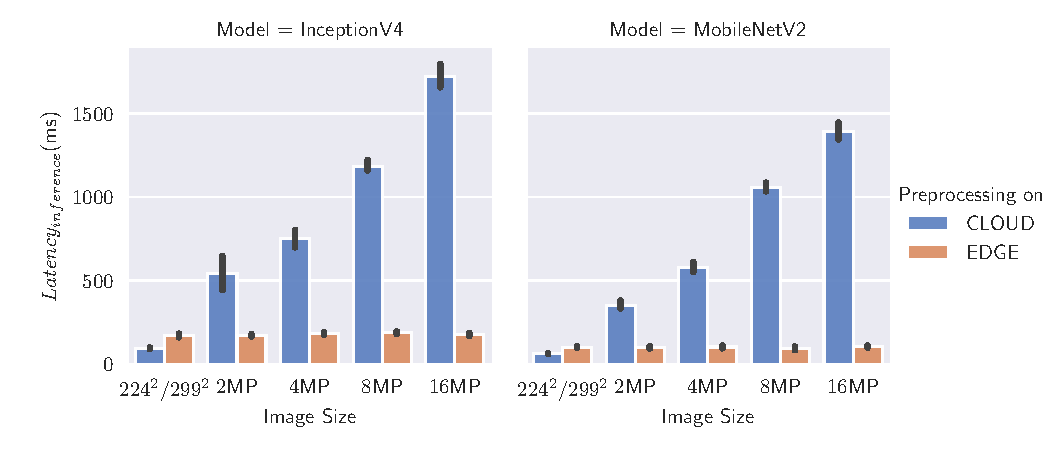
\includegraphics[width=0.95\textwidth]{./Bilder/single_plots/cloud_inference_plots/Cloud_Inference_Latency.pdf}
\caption{Cloud Inference -  $Latency_{inference}$}
\label{fig:cloudInferenceInferenceLatency}
\end{figure}



\begin{figure}[!htb]
\centering
\begin{subfigure}[b]{0.95\textwidth}
   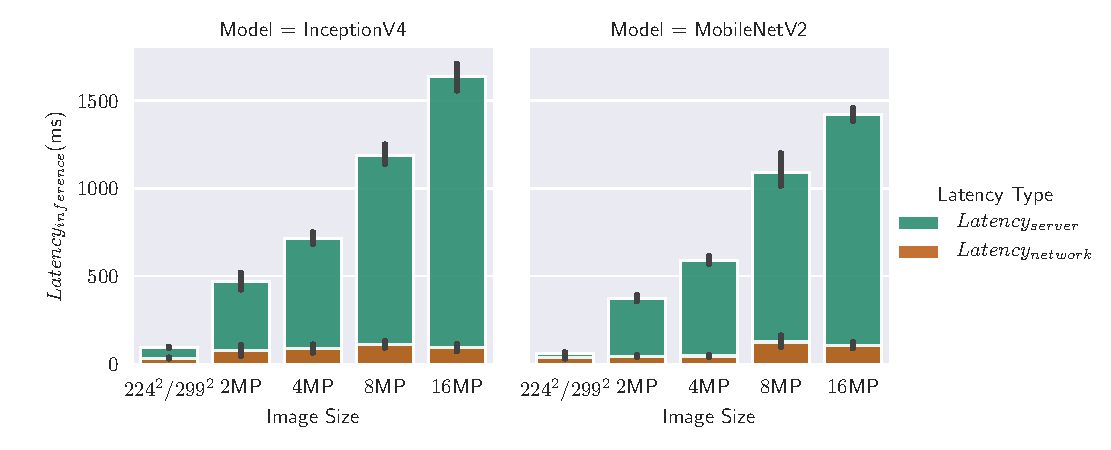
\includegraphics[width=1\linewidth]{./Bilder/single_plots/cloud_inference_plots/Cloud_Server_+_NetworkLatencies_cloudprepro.pdf}
   \caption{Cloud Preprocessing}
   \label{fig:CloudInferenceratioCloudtotal} 
\end{subfigure}

\begin{subfigure}[b]{0.95\textwidth}
   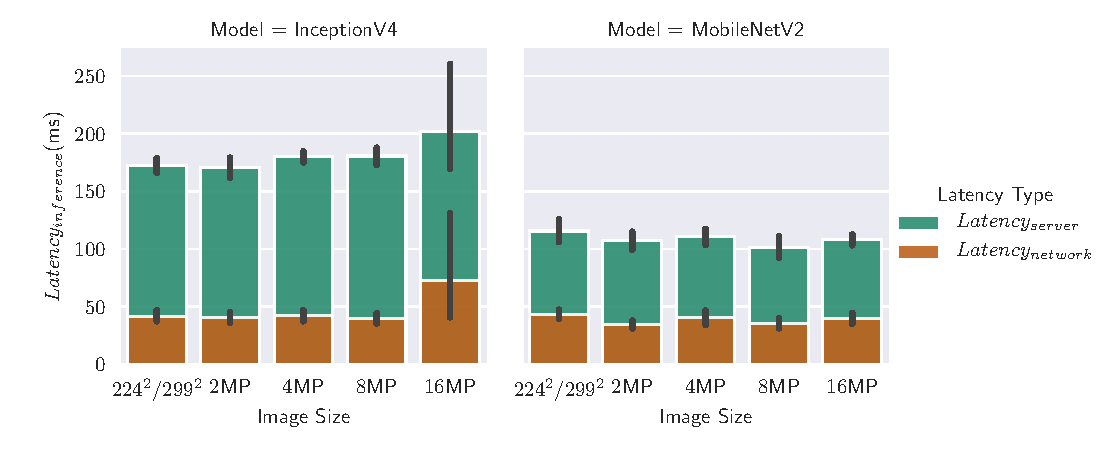
\includegraphics[width=1\linewidth]{./Bilder/single_plots/cloud_inference_plots/Cloud_Server_+_NetworkLatencies_edgeprepro.pdf}
   \caption{Edge Preprocessing}
   \label{fig:CloudInferenceRatioEdgetotal}
\end{subfigure}

\caption{Cloud Inference -  $Latency_{inference}$ including $Latency_{network}$ and $Latency_{server}$}
\end{figure}

\begin{comment}


\begin{figure}[!htb]
\centering
\begin{subfigure}[b]{0.95\textwidth}
   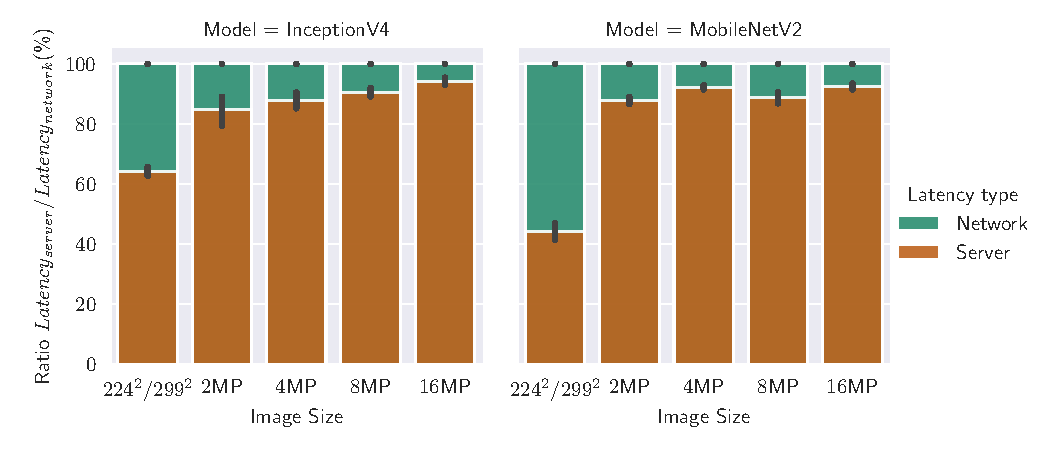
\includegraphics[width=1\linewidth]{./Bilder/single_plots/cloud_inference_plots/Cloud_ratio_server_total_latency_(cloud_prepro).pdf}
   \caption{Cloud Preprocessing}
   \label{fig:CloudInferenceratioCloudrel} 
\end{subfigure}

\begin{subfigure}[b]{0.95\textwidth}
   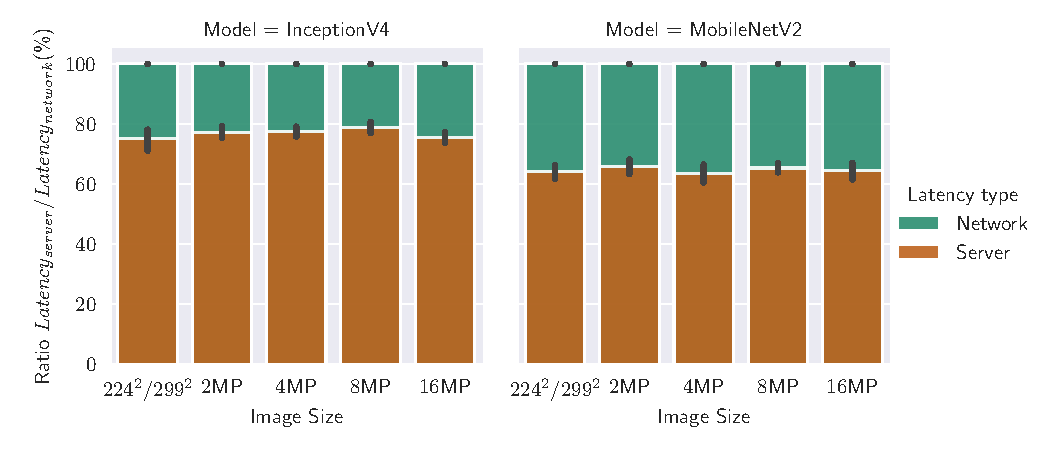
\includegraphics[width=1\linewidth]{./Bilder/single_plots/cloud_inference_plots/Cloud_ratio_server_total_latency_(edge_prepro).pdf}
   \caption{Edge Preprocessing}
   \label{fig:CloudInferenceRatioEdgerel}
\end{subfigure}

\caption{Cloud Inference -  Ratio between $Latency_{network}$ and $Latency_{server}$}
\end{figure}
\end{comment}


\begin{figure}[!htb]
\centering
\begin{subfigure}[b]{0.95\textwidth}
   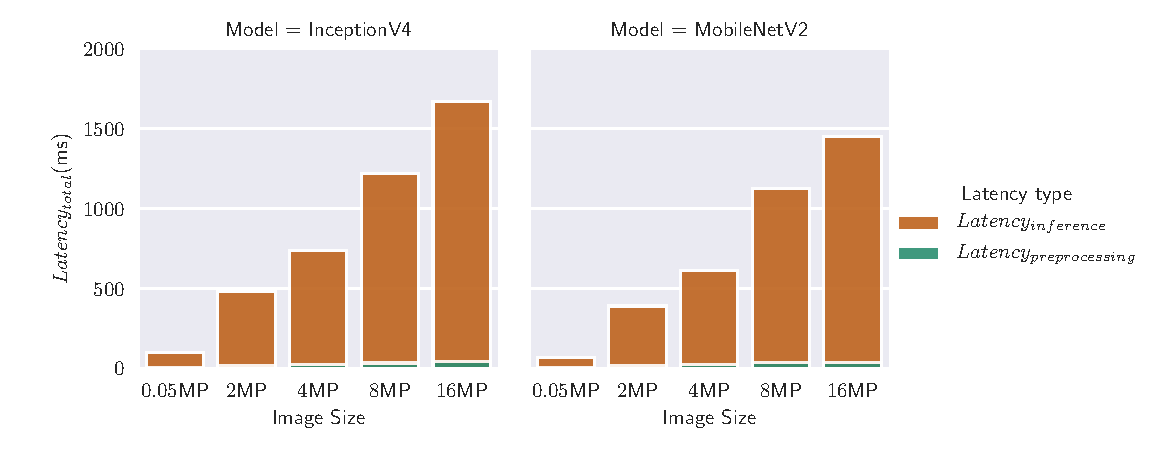
\includegraphics[width=1\linewidth]{./Bilder/single_plots/cloud_inference_plots/Cloud_Preprocessing_Inference_Comb_cloud_prepro.pdf}
   \caption{Cloud Preprocessing}
   \label{fig:CloudInference+PreproCloud} 
\end{subfigure}

\begin{subfigure}[b]{0.95\textwidth}
   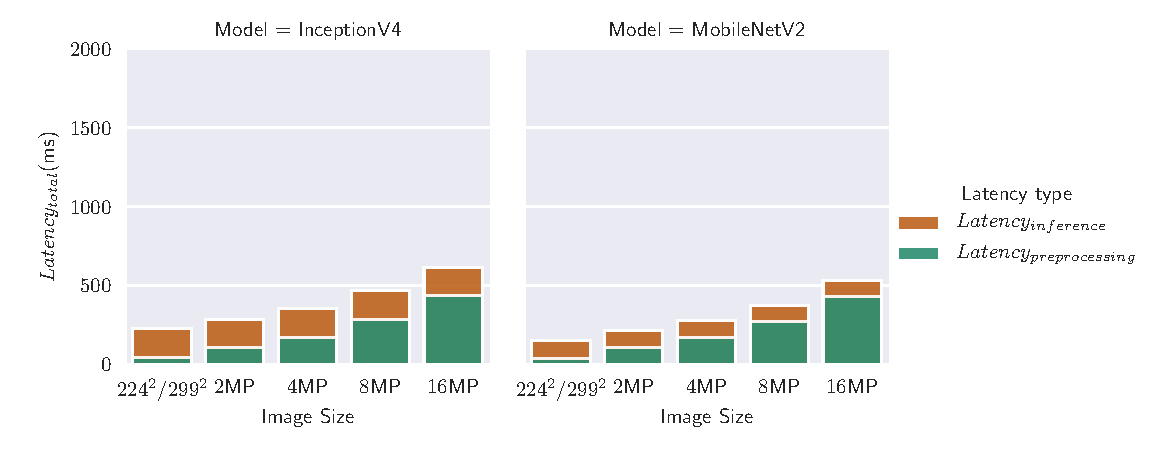
\includegraphics[width=1\linewidth]{./Bilder/single_plots/cloud_inference_plots/Cloud_Preprocessing_Inference_Comb_edge_prepro.pdf}
   \caption{Edge Preprocessing}
   \label{fig:CloudInference+PreproEdge}
\end{subfigure}

\caption{Cloud Inference -  $Latency_{preprocessing}$ and $Latency_{inference}$ combined}
\end{figure}

Figures \ref{fig:CloudInferenceReceivedData} and \ref{fig:CloudInferenceTransmittedData} show the data transmitted and received from the edge client to the cloud-backend server for the different image sizes and preprocessing options.
For edge processed image the mean transmitted data is $1061.9/608.7$KB for InceptionV4/MobileNetV2 and $16.7/10.3$KB data received by the respective models.
Therefore $299^2$ images require $453.2$ kilobytes more than $224^2$ images.
For cloud preprocessing $Data_{transmitted}$ the amount of data sent is at maximum $100$KB larger than the sizes of the \emph{PNG} images ($224^2$: $83$KB, $299^2$: $141$KB, $2$MP: $2411$KB, $4$MP: $4309$KB, $8$MP: $7515$KB,  $16$MP: $10077$KB).
For both edge and cloud preprocessing the $Data_{received}$ rises for rising $Data_{transmitted}$ values, since the communication between server and client is done via TCP, thus more sent data results in more packages resulting in more ACK signals getting sent back to the client.
%%NR:[114.5] transmitted
%%NR:[3.] received
%%2MP:[2446.2] transmitted
%%2MP:[38.2] received
%%4MP:[4365.5] transmitted
%%4MP:[64.8] received
%%8MP:[7603.6] transmitted
%%8MP:[114.9] received
%%16MP:[10176.8] transmitted
%%16MP:[141.4] received
%299 png kleiner als 299 preporcessing
%%mit echter bildgröße abgleichen
%2MP($1732\times1155$, $2411$KB), 4MP($2449\times1633$, $4309$KB), 8MP($3464\times2309$, $7515$KB) and 16MP($4899\times3266$, $10077$KB) ($224\times224$, $83$KB or $299\times299$, $141$KB


\begin{figure}[!htb]
\centering
\begin{subfigure}[b]{0.95\textwidth}
   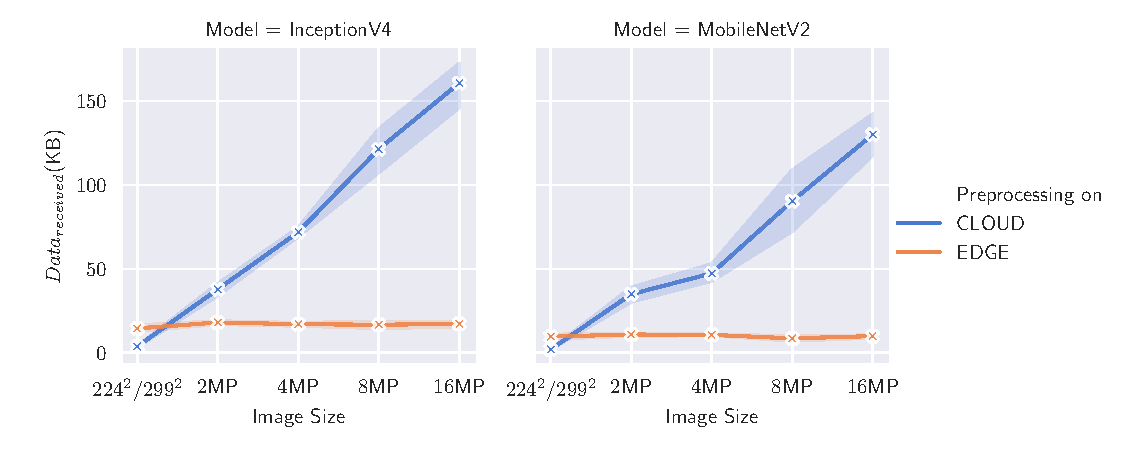
\includegraphics[width=1\linewidth]{./Bilder/single_plots/cloud_inference_plots/Cloud_Inference_Received_Data.pdf}
   \caption{$Data_{received}$}
   \label{fig:CloudInferenceReceivedData} 
\end{subfigure}

\begin{subfigure}[b]{0.95\textwidth}
   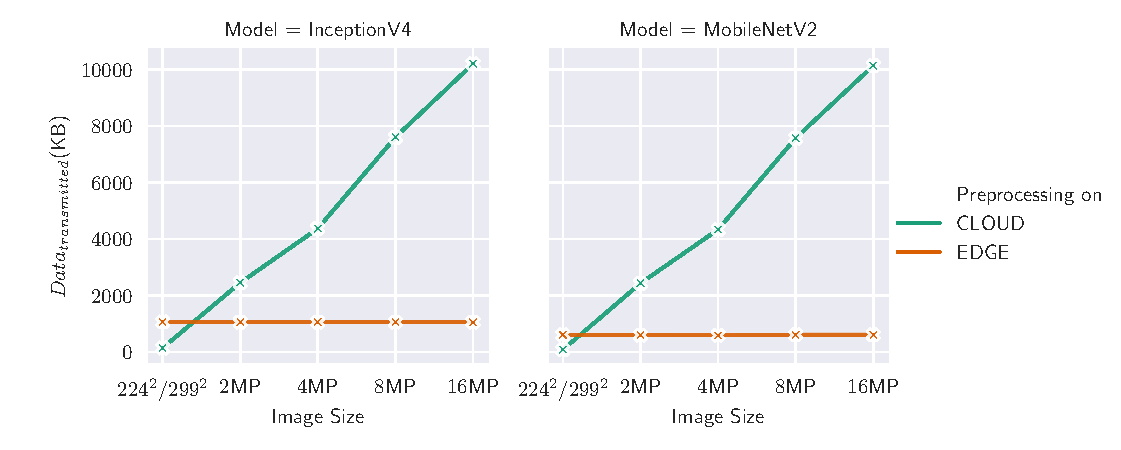
\includegraphics[width=1\linewidth]{./Bilder/single_plots/cloud_inference_plots/Cloud_Inference_Transmitted_Data.pdf}
   \caption{$Data_{transmitted}$}
   \label{fig:CloudInferenceTransmittedData}
\end{subfigure}

\caption{Cloud Inference -  $Data_{received}$ vs. $Data_{transmitted}$}
\end{figure}

\FloatBarrier
\paragraph{Cloud Inference - Key Takeaways}
%cloud prepro less preprocessing memory and latency
%cloud prepro more inference memory
%cloud preprocessing very slow for large image sizes
%edge prepro faster for all image sizes except 224/299
%network not a bottlneck
%resize binlinear bad implementation?
\emph{
\begin{itemize}
    \item Preprocessing on the cloud in comparison to edge preprocessing causes:
    \begin{itemize}
        \item $20\times$ faster $Latency_{preprocessing}$ for $224^2/299^2$ images
        \item $10\times$ faster $Latency_{preprocessing}$ for $16$MP images
        \item $1.28\times$ less $Memory_{preprocessing}$ for $16$MP images
    \end{itemize}
    \item Inference on the cloud including preprocessing in comparison to cloud inference without preprocessing causes:
    \begin{itemize}
        \item $2.3\times$ faster InceptionV4/MobileNetV2 $Latency_{total}$ for $224^2/299^2$ images
        \item $2.7\times$ slower InceptionV4/MobileNetV2 $Latency_{total}$ for $16$MP images
        \item $0.97\times$ less $Memory_{inference}$ for $224^2/299^2$ images
        \item $1.14\times$ more $Memory_{inference}$ for $16$MP images
    \end{itemize}
    \item MobileNetV2 is up to $1.75\times$ faster than InceptionV4 for smaller images, but shrinking to around $10\%$ faster for large image in case of cloud preprocessing.
    \item Network is accountable for up to $50\%$ of $Latency_{inference}$ for $224^2/299^2$ images and networks, but less than $30\%$ for larger images and network for both cloud and edge preprocessing.
\end{itemize}
\begin{itemize}[leftmargin=4em]
 \renewcommand{\labelitemi}{$\Rightarrow$}
 \item Edge Preprocessing has faster $Latency_{total}$ latencies for all image sizes except $224^2/299^2$.
\end{itemize}
}%emph end


\subsection{Edge vs. Cloud Inference}
Previous two sections presented the results for both edge and cloud inference.
Now, the results of the cloud and the edge inference with batch size one, including preprocessing, are compared against each other.
First preprocessing and inference are evaluated separately and afterwards both of the steps combined. 
Each plot of this section contains five subplots, one for each image sizes, the x-axis contains the deep learning model, while the y-axis displays the various performance metrics. 
The legend used in all those plots in explained in table \ref{table:legendPlots}.
\begin{table}[!htb]
\newcommand\crule[3][black]{\textcolor{#1}{\rule{#2}{#3}}}
\centering
\caption{Explanation of the plot legends}
\label{table:legendPlots}
\begin{tabular}{@{}lll@{}}
\toprule
Inference on & Description & Color \\ \midrule
\begin{tabular}[c]{@{}l@{}}Inf on:CLOUD;\\ Prepro on:CLOUD\end{tabular} & \begin{tabular}[c]{@{}l@{}}Inference as well as preprocessing is done on the\\ cloud-backend.\end{tabular} &  \crule[gruen]{0.8cm}{0.8cm}\\
\begin{tabular}[c]{@{}l@{}}Inf on:CLOUD;\\ Prepro on:EDGE\end{tabular} & \begin{tabular}[c]{@{}l@{}}Inference is done on cloud-backend, but images are \\ preprocessed on edge beforehand.\end{tabular} &  \crule[orangedunkel]{0.8cm}{0.8cm}\\
\begin{tabular}[c]{@{}l@{}}Inf on:EDGE;\\ Prepro on:EDGE\end{tabular} & \begin{tabular}[c]{@{}l@{}}Inference as well as preprocessing is done on the\\ edge.\end{tabular} & \crule[lila]{0.8cm}{0.8cm} \\ \bottomrule
\end{tabular}
\end{table}

Not that for the quantized MobileNetV2 we only conduct edge inference experiments, thus no cloud inference results for this model can be seen in the plots of this section.
\subsubsection{Preprocessing}

Figures \ref{fig:EdgeVsCloudPreproMemory}, \ref{fig:EdgeVsCloudPreproLat} and \ref{fig:CloudEdgePreproCPU} report the preprocessing metrics $Memory_{preprocessing}$, $Latency_{preprocessing}$ and $CPU_{preprocessing}$.

%Memory
\paragraph{$\mathbf{Memory_{preprocessing}}$}
Both edge preprocressing options, for either edge inference or cloud inference, have very similar memory consumption results with the cloud inference mean values being at most $5.5\%$ higher from the edge inference values for all image sizes.
This due to the fact that both options share most of the preprocessing steps, the only difference is that in case of cloud inference with edge preprocessing the \emph{ByteBuffer}, containing the preprocessed image, gets used to build the \emph{PredictRequest} for TensorFlow Serving. 
For edge inference no such step is needed as the \emph{ByteBuffer} can be directly be used to call the run function of the TensorFlow Lite interpreter, which starts the inference process at the edge.
Thus the $5.5\%$ overhead in memory can be explained by the additional \emph{PredictRequest} object that has to loaded into memory for cloud inference.

In case of small images the memory consumption of cloud preprocessing is very close to its edge preprocessing counter-part, the larger the image the larger the memory difference.
While the difference is only $1.9\%$ for an $224^2/299^2$ image ($114.53/116.69$MB), the difference grows to an $22.5\%$ decrease ($177.8/137.8$MB)in memory for $16$MP images ($2$MP: $1.1\%$, $4$MP: $7.9\%$, $8$MP: $9.9\%$).
This difference is caused by the fact that for cloud preprocessing only the compressed \emph{PNG} gets loaded into memory, which is a lot smaller than the decoded image, especially for large images such as the $16$MP image.

When comparing the different models InceptionV4 ($140.1$MB) consumed about $7.9$MB more $Memory_{preprocessing}$ than MobileNetV2 ($132.2$MB), or about $6\%$, independent of image size or inference mode (edge inference, cloud inference with edge preprocessing and cloud inference with cloud preprocessing).
Edge inference of the quantized version of MobileNetV2 causes the same memory consumption as the non quantized version.
When differentiating between the different image sizes and inference modes the difference is always between $4-8\%$, except for cloud preprocessing of an $224^2/299^2$ image, where the difference rises to $10\%$ ($11.35$MB). This is due to the fact that MobileNetV2 preprocesses $224^2$ images and InceptionV4 $299^2$ images.

%Latency
\paragraph{$\mathbf{Latency_{preprocessing}}$}
The preprocessing latency results are similar to the memory results. Both edge preprocessing options are very similar in performance, while cloud preprocessing performs better, but in case of latency the difference is larger.

The difference between the edge preprocessing options (cloud inference with edge preprocessing and edge preprocessing) is at most $4.9\%$ ($5.1$ms) across all images sizes (not differentiating between the different models).

When comparing edge preprocessing to cloud preprocessing the latency gap for $224^2/299^2$ images is a factor of $20$ in the favor of cloud preprocessing ($1.9/38.2$ms). For larger image sizes this gap shrinks, but still amounts $11\times$ for $16$MP images ($37.9/430.78$ms).

The different models have little to no impact on the preprocessing when comparing same images sizes.
For cloud preprocessing the MobileNetV2 and InceptionV4 differ at most $4.9$ms (for $8$MP, all other image size are below that for both relative and total difference). This difference is not significant since the standard deviation for the mean values is more than twice as high for both models.
%%difference between models for edge preporcessing
%%%model compare
%cloud prepro no diff for models
%%diff for NR large for edge prepro -> normalizing more work
This is also true for edge preprocessing for all image sizes, regardless of edge or cloud inference.
Although the difference between the models is up to $29\%$ or $10.3$ms ($224^2/299^2$ image), the speedup is not significant as the standard deviation for both models is above $9$ms.

%CPU
\paragraph{$\mathbf{CPU_{preprocessing}}$}
Looking at the CPU usages in figure \ref{fig:CloudEdgePreproCPU} it can be seen that the variance of all inference modes, models and images sizes is too large to make conclusions, although there is a indication that cloud preprocessing causes lower usages.
Overall it can be stated that all usages are around $12.5\%$. This makes sense since the preprocessing of a single image is done on a single thread, thus running on one core and since the OnePlus 6T has 8 cores, the full utilization of a single core causes an overall $CPU_{preprocessing}$  usage of $12.5\%$. 
This infers that the preprocessing uses $100\%$ of a single core, especially for large images.

\begin{figure}[!htb]
\centering
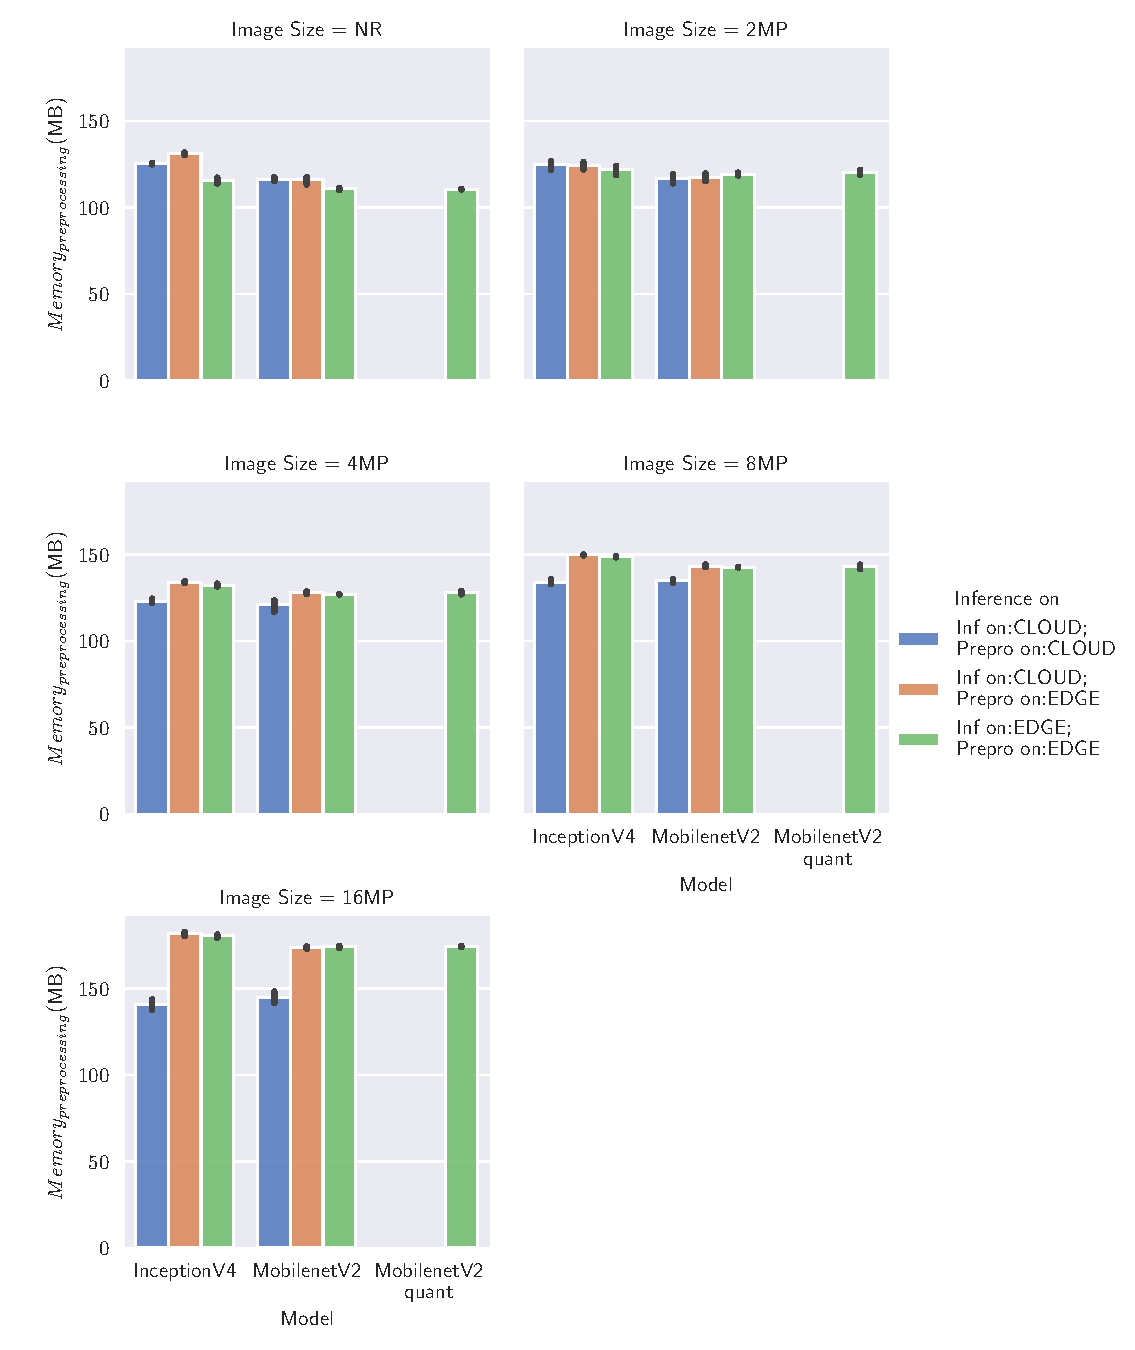
\includegraphics[width=0.95\textwidth]{./Bilder/single_plots/edge_vs_cloud_plots/Edge_vs_Cloud_Inference_Preprocessing_Memory.pdf}
\caption{Edge vs. Cloud Inference -  $Memory_{preprocessing}$}
\label{fig:EdgeVsCloudPreproMemory}
\end{figure}

\begin{figure}[!htb]
\centering
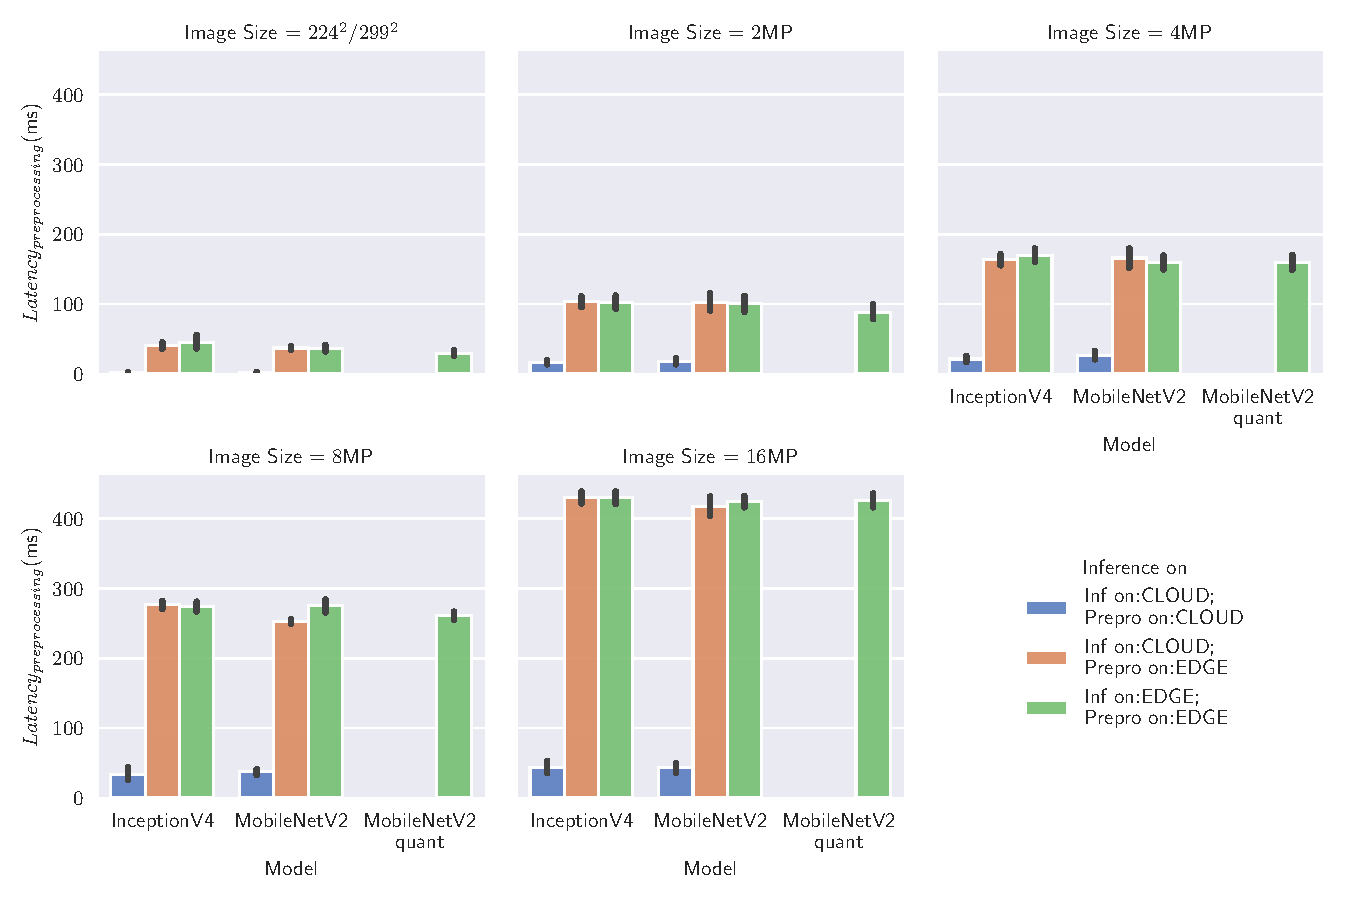
\includegraphics[width=0.95\textwidth]{./Bilder/single_plots/edge_vs_cloud_plots/Edge_vs_Cloud_Inference_Preprocessing_Latencies.pdf}
\caption{Edge vs. Cloud Inference -  $Latency_{preprocessing}$}
\label{fig:EdgeVsCloudPreproLat}
\end{figure}

\FloatBarrier
\subsubsection{Inference}
\paragraph{$\mathbf{Memory_{inference}}$}
Figure \ref{fig:EdgeVsCloudInferenceMemory} reports $Memory_{inference}$ for all inference modes, models and image sizes.
Image size has no impact on the memory consumption during inference, where image have been previously preprocessed, which is logical, since the preprocessed image have the same memory constraints regardless of the size before preprocessing.
In contrary cloud inference with cloud preprocessing memory consumption is impacted by different image sizes, since the images are not preprocessed and thus larger images are being sent to the server.
$16$MP images use $19\%$ more memory for InceptionV4 in comparison to a $224^2/299^2$ image and $13\%$ more for MobileNetV2.


While different images sizes only have a small impact on $Memory_{inference}$ different inference modes (edge inference, cloud inference with either edge or cloud preprocessing) do have a large impact, especially in the case of the large InceptionV4 network.
Edge Inference with InceptionV4 consumes more than twice ($2.2\times$) as much memory than both cloud inference options.

While cloud inference for InceptionV4 can half memory consumption, MobileNetV2 does not profit nearly as much from cloud inference, as edge inference with MobileNetV2 only uses $10.5\%$ ($13.6$MB) more an average (independent of image size) than cloud inference with edge preprocessing due to its small model size.
Edge inference with MobileNetV2 even uses less memory than cloud inference with cloud preprocessing for $16$MP images, as the un-preprocessed image consumes more memory than the loaded model. 

The quantization of MobileNetV2 has no significant impact on memory consumption.


%inception on egde much more, mobilenet nearly equal (more for small images, less forlarge images than cloud prepro)
\paragraph{$\mathbf{Latency_{inference}}$}
figure \ref{fig:EdgeVsCloudInferenceLat}

%beide cloud optionen schneller bei 224/299 inceptionV4
%bei mobilenet cliud prepro schneller, edge schneller als cloud with edge prepro
%quantized faster than rest by far (no network overhead etc)
%faster image size servere impact on cloud inference with cloud preprocessing

\paragraph{$\mathbf{CPU_{inference}}$}
%not interesting
\paragraph{$\mathbf{Throughput_{inference}}$}

\paragraph{$\mathbf{Throughput_{total}}$}


\begin{figure}[!htb]
\centering
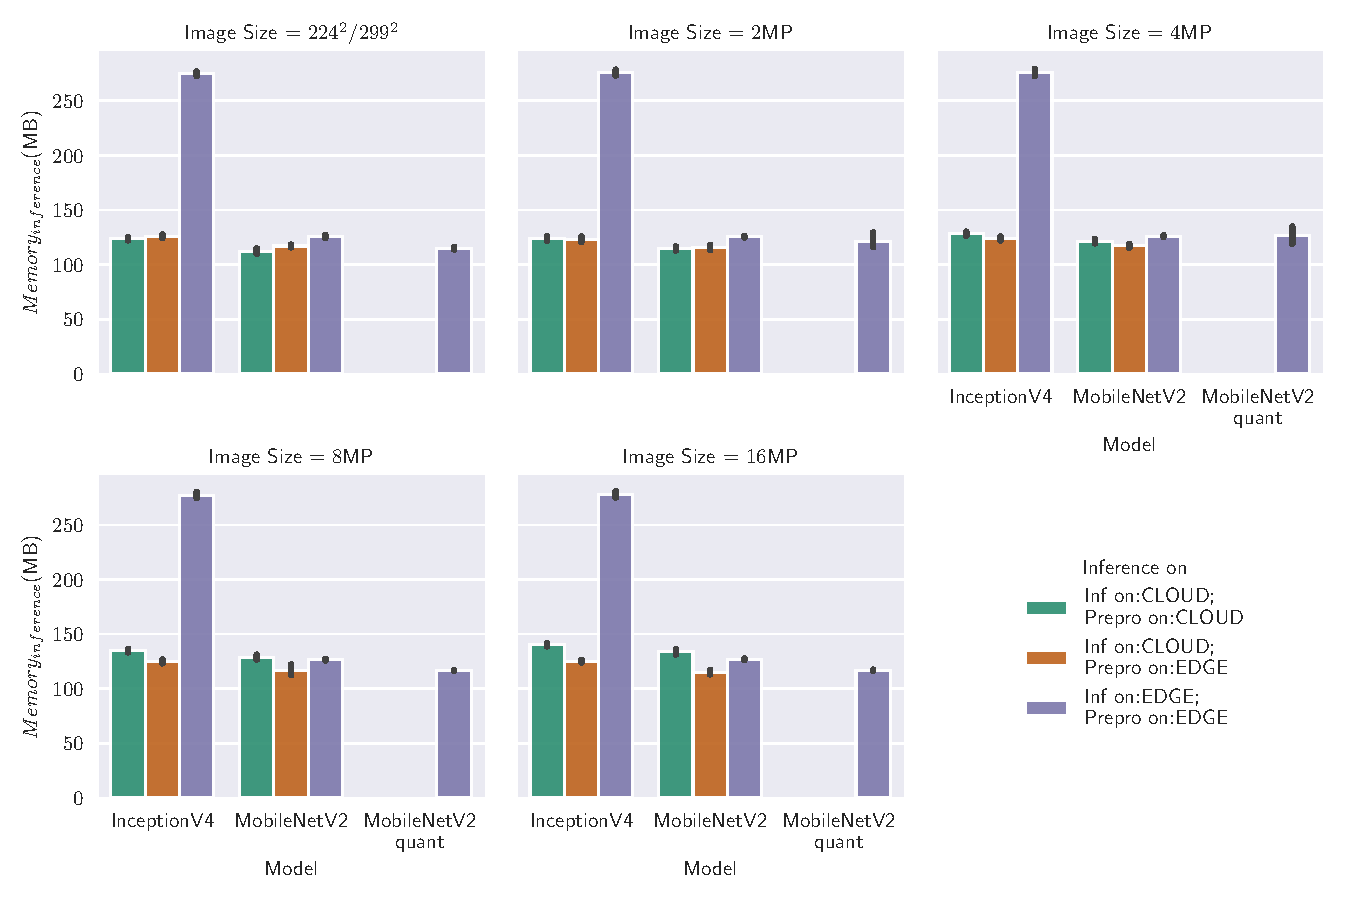
\includegraphics[width=0.95\textwidth]{./Bilder/single_plots/edge_vs_cloud_plots/Edge_vs_Cloud_Inference_Inference_Memory.pdf}
\caption{Edge vs. Cloud Inference -  $Memory_{inference}$}
\label{fig:EdgeVsCloudInferenceMemory}
\end{figure}
\begin{figure}[!htb]
\centering
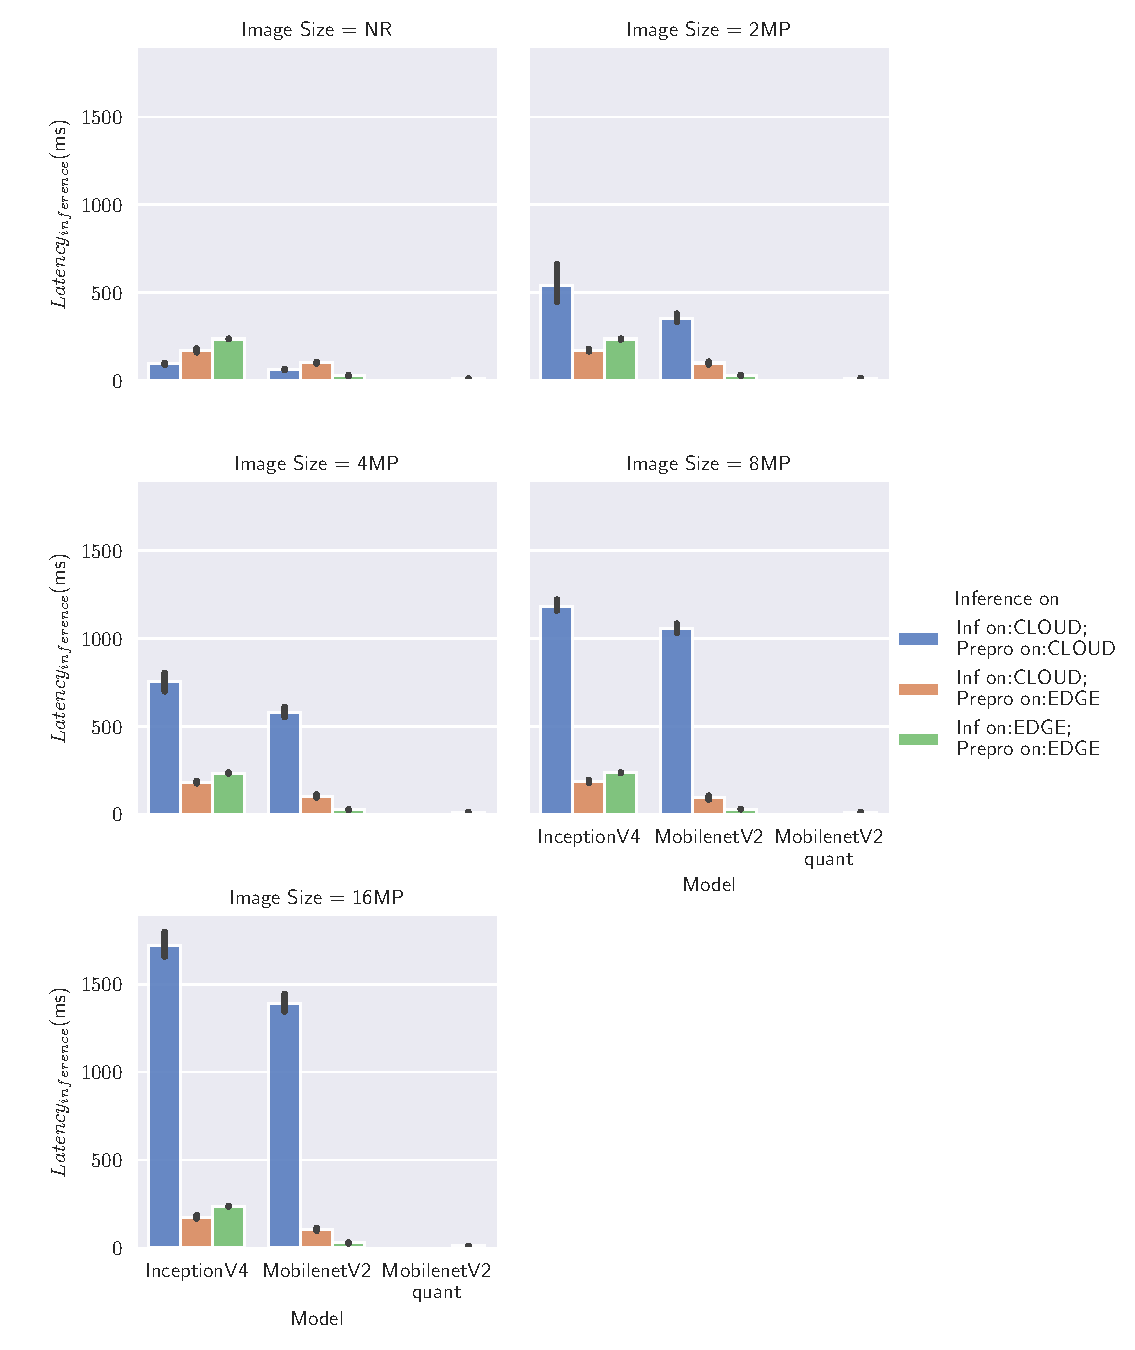
\includegraphics[width=0.95\textwidth]{./Bilder/single_plots/edge_vs_cloud_plots/Edge_vs_Cloud_Inference_Inference_Latencies.pdf}
\caption{Edge vs. Cloud Inference -  $Latency_{inference}$}
\label{fig:EdgeVsCloudInferenceLat}
\end{figure}

\begin{figure}[!htb]
\centering
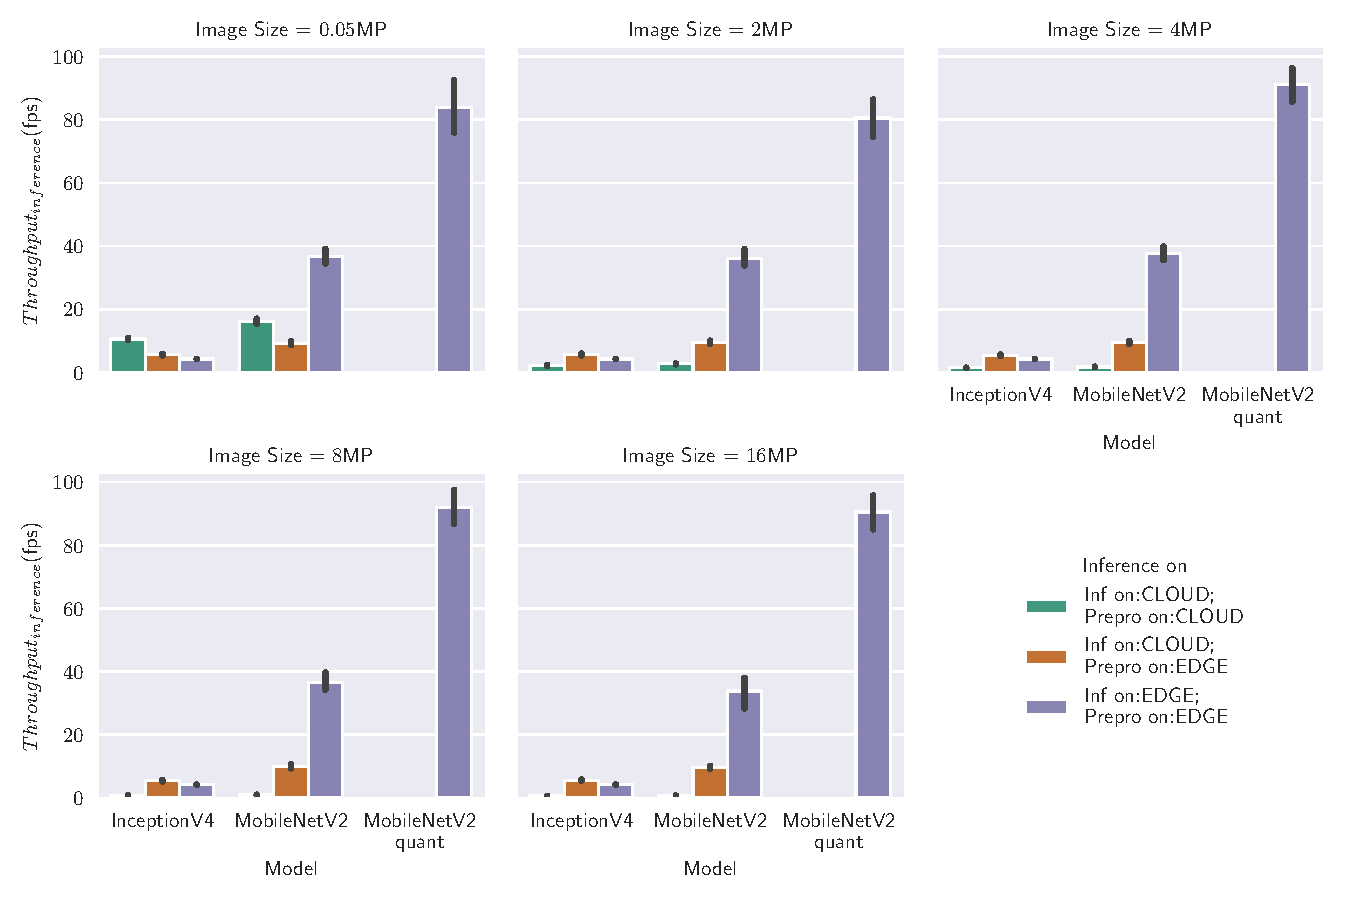
\includegraphics[width=0.95\textwidth]{./Bilder/single_plots/edge_vs_cloud_plots/Edge_vs_Cloud_Inference_Throughput_without_Preprocessing.pdf}
\caption{Edge vs. Cloud Inference -  $Throughput_{inference}$ - higher is better}
\label{fig:EdgeVsCloudinferneceThroughput}
\end{figure}

\begin{figure}[!htb]
\centering
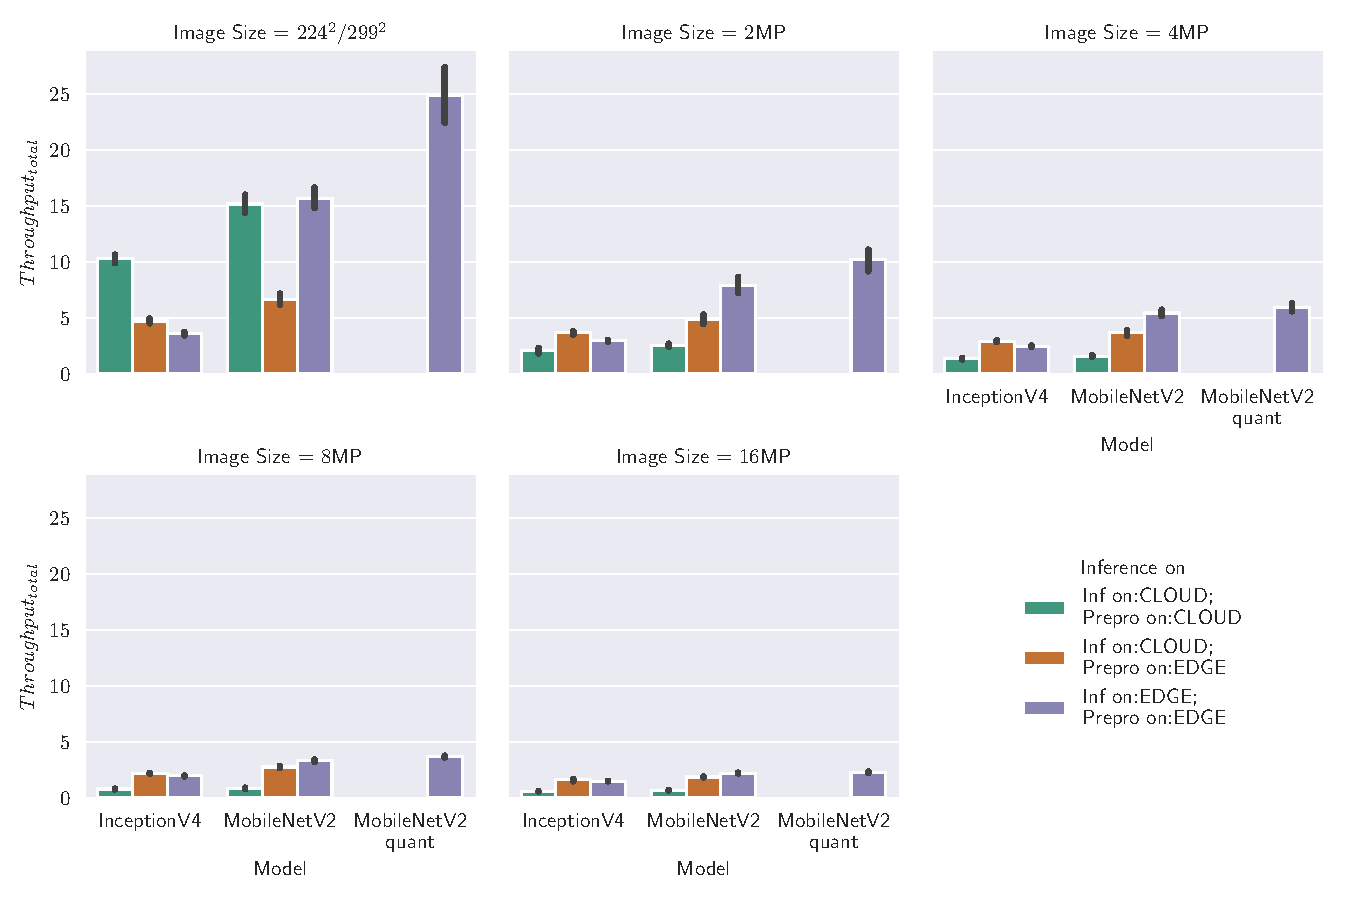
\includegraphics[width=0.95\textwidth]{./Bilder/single_plots/edge_vs_cloud_plots/Edge_vs_Cloud_Inference_Throughput_with_Preprocessing.pdf}
\caption{Edge vs. Cloud Inference -  $Throughput_{total}$ (Inference + Preprocessing)}
\label{fig:EdgeVsCloudTotalThroughput}
\end{figure}

\FloatBarrier
\paragraph{Edge vs. Cloud Inference - Key Takeaways}
\emph{
\begin{itemize}
    \item x
    \item y
    \item z
\end{itemize}
}

\subsection{Effect of larger Batch Sizes}
\label{chap:resultsBatchSize}
So far we only reported the results of the of the experiments with batch size of one, but in this section we present the results for a batch size equal or larger than one.
Increasing the batch size  is supposed to increase throughput at the expense of low latencies.
Since the TensorFlow Lite of the used MobileNetV2 version does not allow batch sizes larger than one, edge inference experiments with these models are omitted from this section.

Since the batch size is added as a new dimension in this section, the plots visualizing the results need to be expanded.
Now the x-axis respresents the various batch sizes and the models are moved to the legend. 
The legend is similar to table \ref{table:legendPlots}, but the model is added as an additional feature to the inference mode.
\subsubsection{Preprocessing}
\begin{figure}[!htb]
\centering
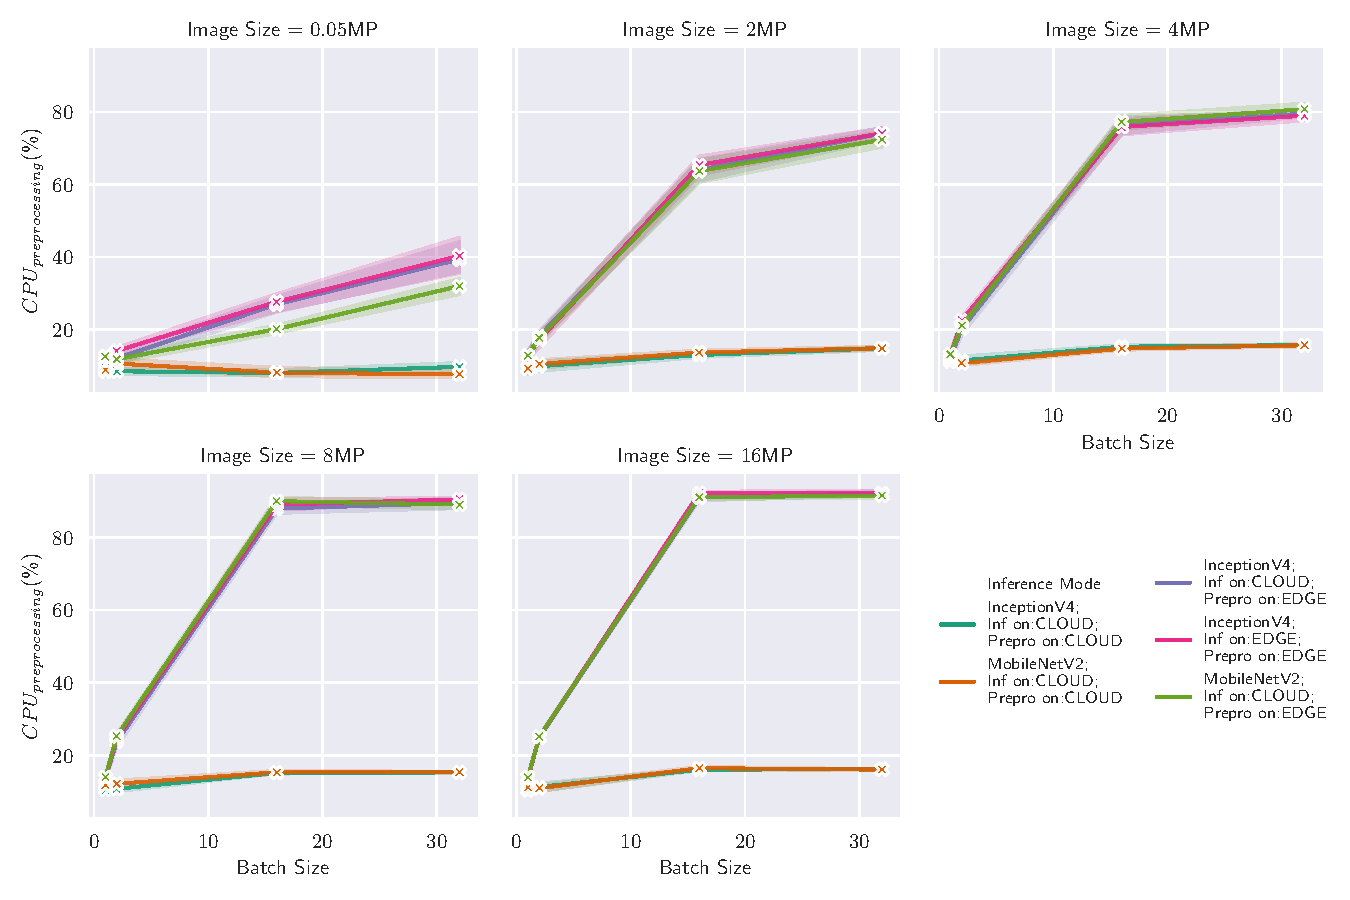
\includegraphics[width=0.95\textwidth]{./Bilder/single_plots/batch_size_plots/Effects_of_Batch_size_Preprocessing_CPU_Usage.pdf}
\caption{Edge vs. Cloud Inference for larger Batch Sizes -  $CPU_{preprocessing}$ - lower is better}
\label{fig:BatchSizePreproCPU}
\end{figure}

\begin{figure}[!htb]
\centering
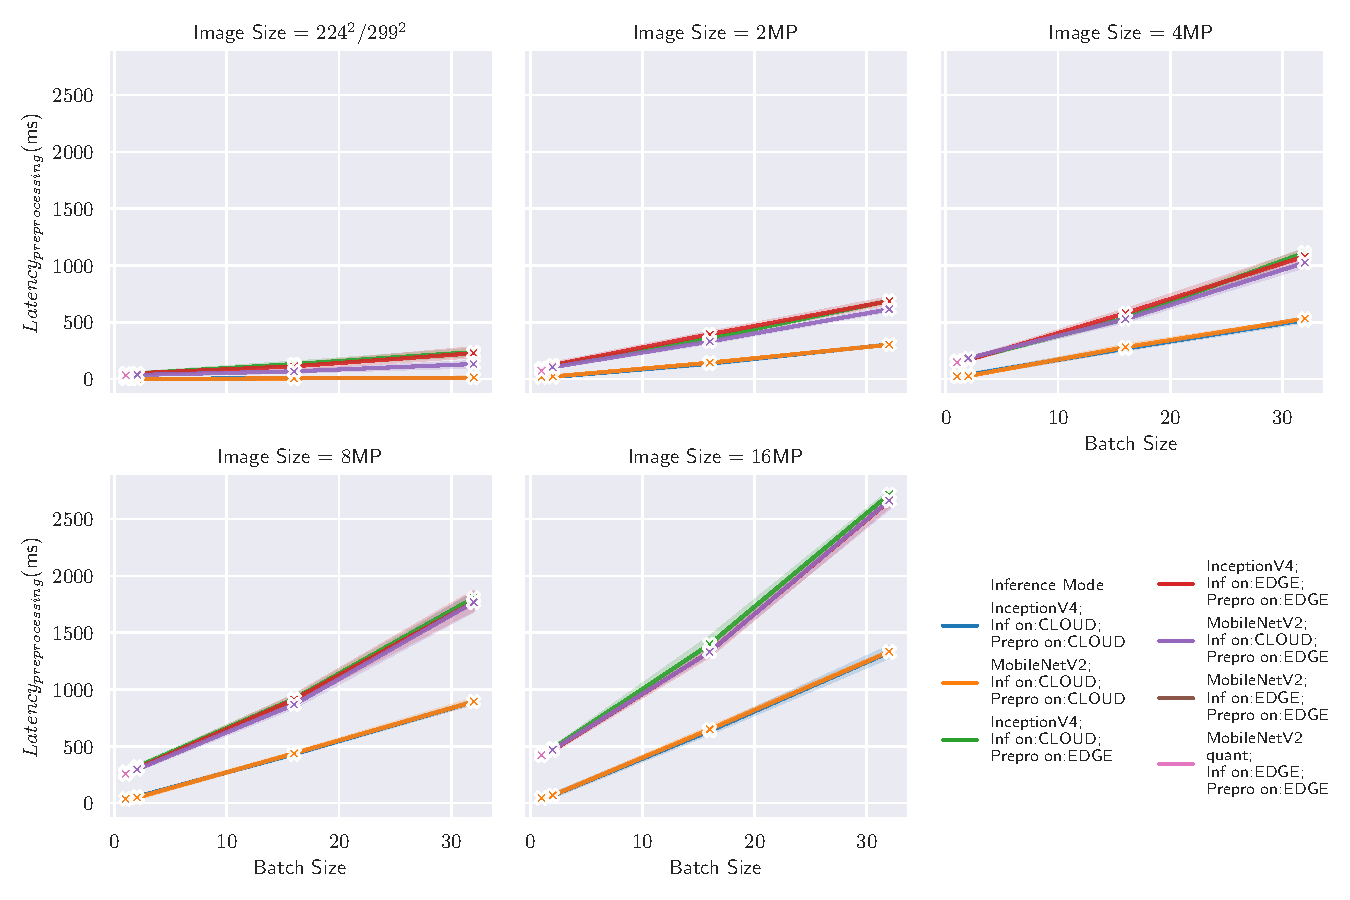
\includegraphics[width=0.95\textwidth]{./Bilder/single_plots/batch_size_plots/Effects_of_Batch_size_Preprocessing_Latencies.pdf}
\caption{Edge vs. Cloud Inference for larger Batch Sizes -  $Latency_{preprocessing}$ - lower is better}
\label{fig:BatchSizePreproLatency}
\end{figure}
\begin{figure}[!htb]
\centering
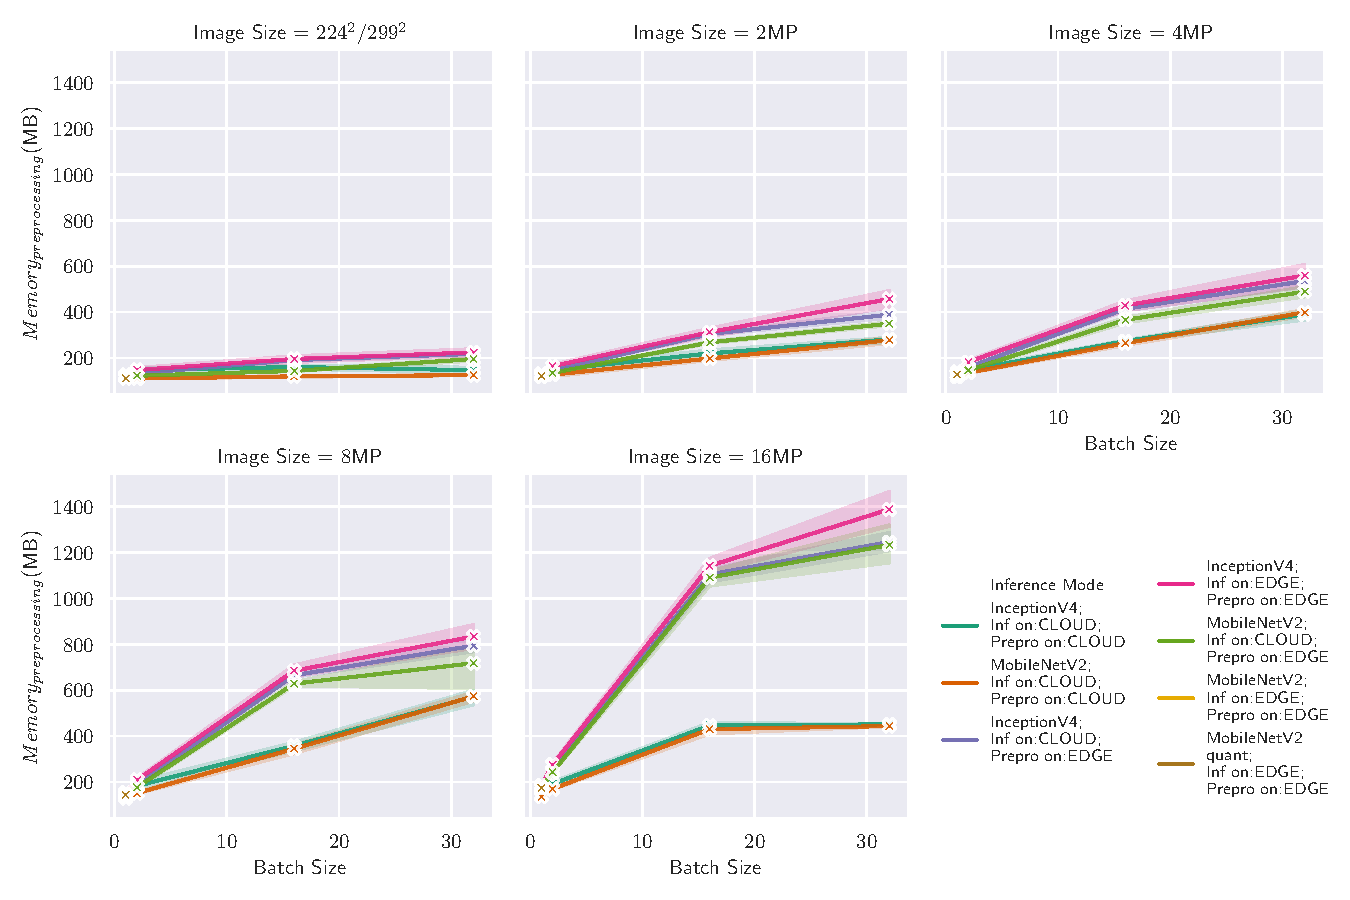
\includegraphics[width=0.95\textwidth]{./Bilder/single_plots/batch_size_plots/Effects_of_Batch_size_Preprocessing_Memory.pdf}
\caption{Edge vs. Cloud Inference for larger Batch Sizes -  $Memory_{preprocessing}$ - lower is better}
\label{fig:BatchSizePreproMemory}
\end{figure}

\FloatBarrier
\subsubsection{Inference}

\begin{figure}[!htb]
\centering
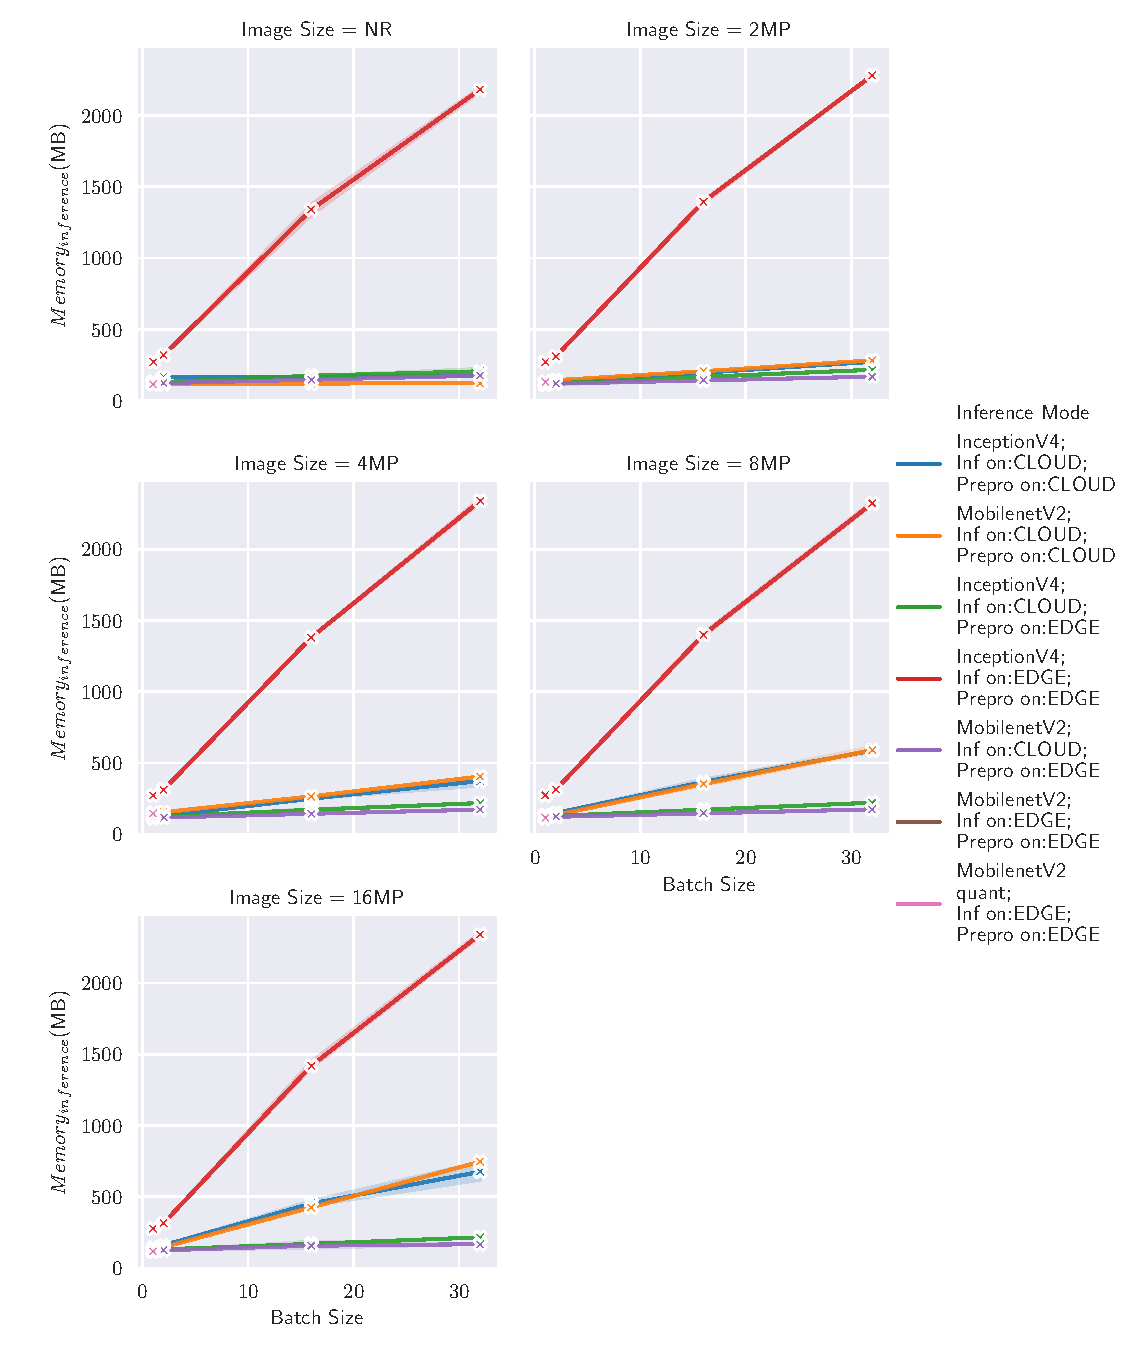
\includegraphics[width=0.95\textwidth]{./Bilder/single_plots/batch_size_plots/Effects_of_Batch_size_Inference_Memory.pdf}
\caption{Edge vs. Cloud Inference for larger Batch Sizes -  $Memory_{inference}$ - lower is better}
\label{fig:BatchSizeInferenceMemory}
\end{figure}
\begin{figure}[!htb]
\centering
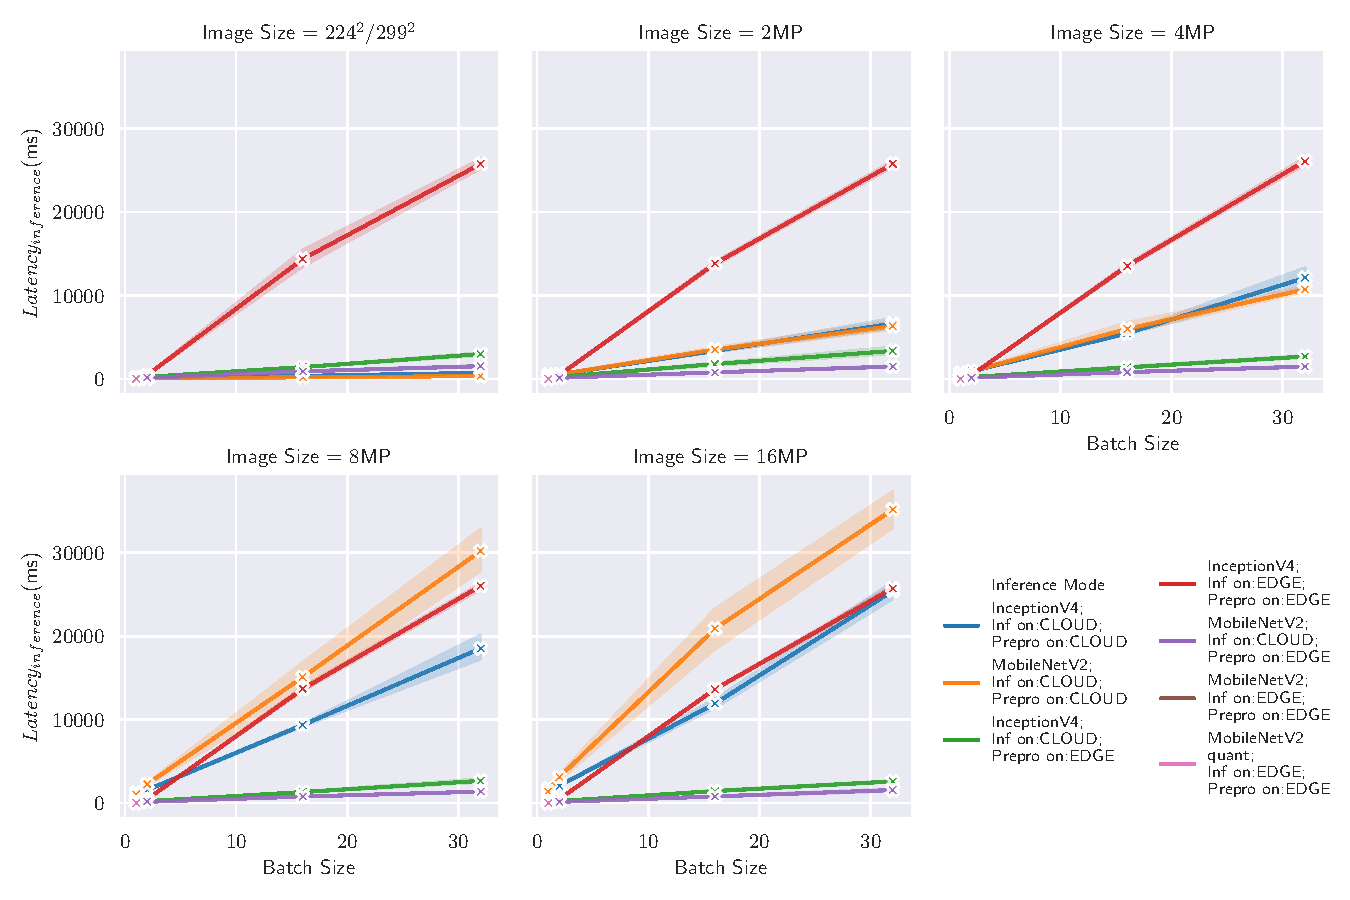
\includegraphics[width=0.95\textwidth]{./Bilder/single_plots/batch_size_plots/Effects_of_Batch_size_Inference_Latencies.pdf}
\caption{Edge vs. Cloud Inference for larger Batch Sizes -  $Latency_{inference}$ - lower is better}
\label{fig:BatchSizeInferenceLatency}
\end{figure}



\begin{figure}[!htb]
\centering
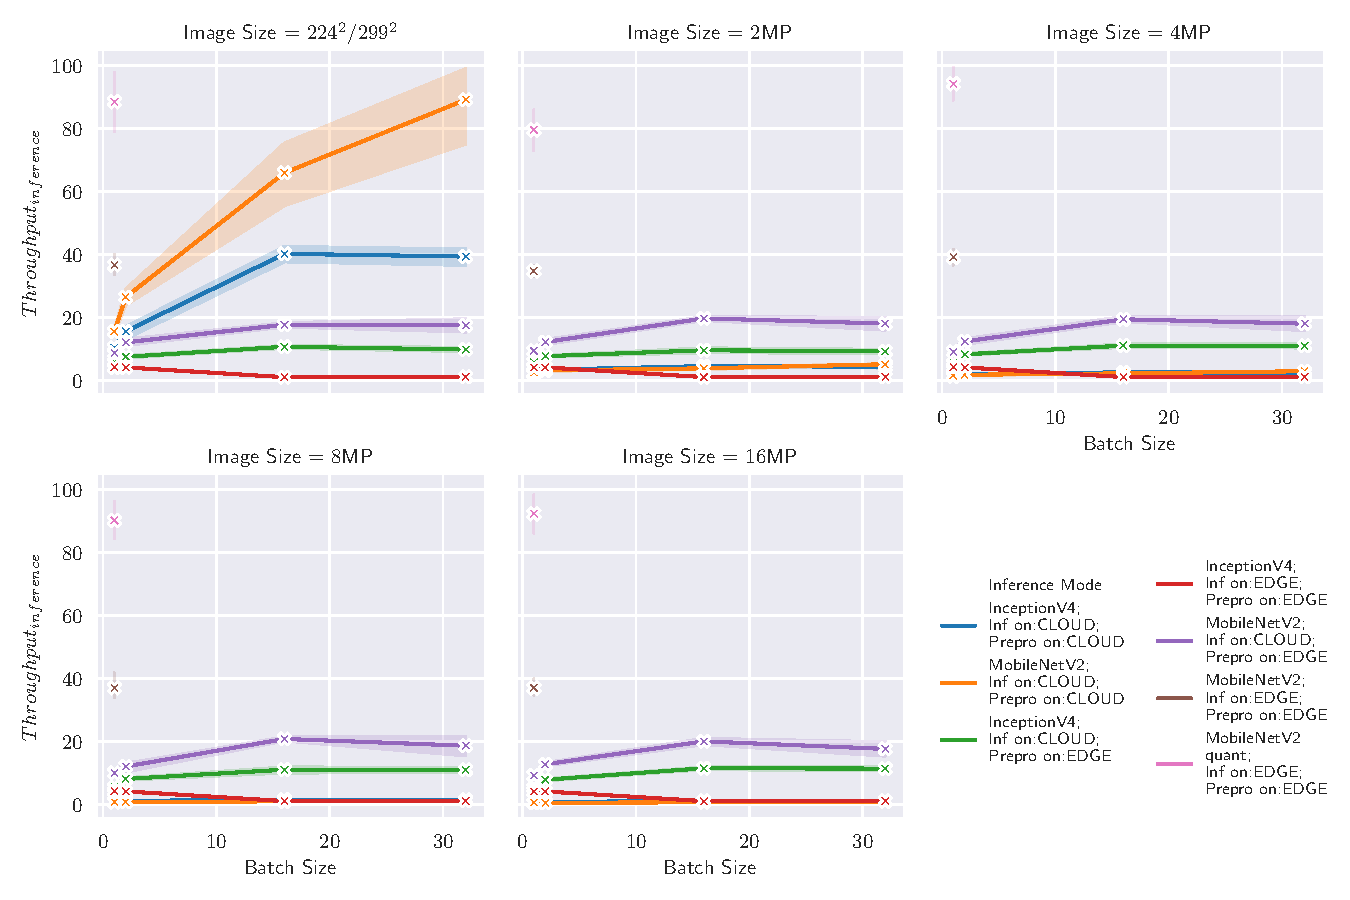
\includegraphics[width=0.95\textwidth]{./Bilder/single_plots/batch_size_plots/Effects_of_Batch_size_Inference_Throughput.pdf}
\caption{Edge vs. Cloud Inference for larger Batch Sizes -  $Throughput_{inference}$ - higher is better}
\label{fig:BatchSizeInferenceThroughput}
\end{figure}
\begin{figure}[!htb]
\centering
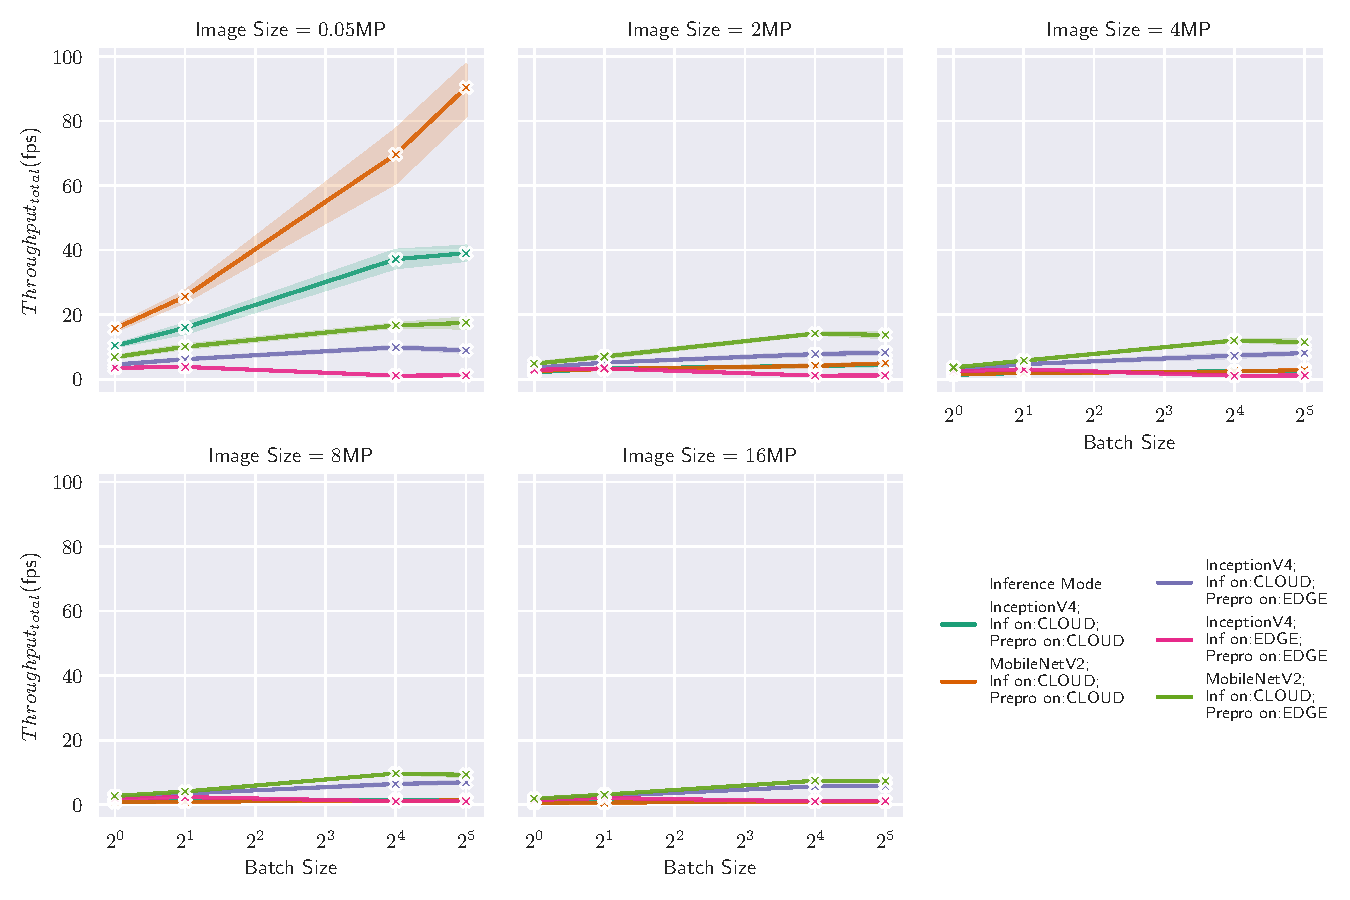
\includegraphics[width=0.95\textwidth]{./Bilder/single_plots/batch_size_plots/Effects_of_Batch_size_Total_Throughput_(Preprocessing_+_Inference).pdf}
\caption{Edge vs. Cloud Inference for larger Batch Sizes -  $Throughput_{total}$ - higher is better}
\label{fig:BatchSizeTotalThroughput}
\end{figure}


\FloatBarrier
\paragraph{Effect of larger Batch Sizes - Key Takeaways}
\emph{
\begin{itemize}
    \item x
    \item y
    \item z
\end{itemize}
}


%%%%%%%%%%%%%%%%%%%%%%%%%
%Überleitung

\endinput 

	\chapter{Methodology Instantiation}
\label{chap:experiments}
In this chapter, we instantiate the methodology defined in the previous section step by step on an image classification use case.

In section \ref{chap:problemSpace} the problem space will be defined, based on the fundamentals of deep learning deployment presented in chapter \ref{chap:fundamentels}, followed by the performance metrics in section \ref{chap:metrics}.


The used infrastructure is presented in section \ref{chap:infrastructure} and includes the used hardware components, at the edge and the cloud, as well as the used inference frameworks for both edge and cloud inference.

Section \ref{chap:parameters} will cover the three deep learning models as well as the different types of input data used for the benchmarks.

Afterwards in section \ref{chap:androidApp} we design a Android benchmark framework, which simulates a real-time AI application using the previously defined workloads and infrastructure. Additionally, the Android application also handles instrumentation of the performance metrics and their collection for later evaluation.

Using this benchmark framework section \ref{chap:benchmarkExec} describes the execution of the benchmark framework, which benchmarks then get evaluated in \ref{chap:Evaluation}.

The benchmarks then get used to train a performance model in section \ref{chap:perfModel}, predicting the runtime latencies of the different deployment options and thus enable the performance model to give recommendations for the deployment.

Finally in chapter \ref{chap:DecisionModel}, the gain understanding of deep learning inference from all the previous steps of the methodology can be used to generate a decision model helping in the decision of optimal deployment option selection for deep learning inference.


\section{Problem Space}
\label{chap:problemSpace}
%AI applications ins spiel bringen
For real-time AI applications to be viable, real-time predictions are essential. Hence the inference performance of deep learning models is a key aspect.
If they performance cannot be achieved at the edge device itself, an alternative solution is the deployment of the deep learning model to a cloud-backend.
To be able to help in this decision, the factors influencing this performance have to be examined in the first place to get a general understanding of deep learning inference.
This section utilizes the in section \ref{chap:fundamentels} presented fundamentals of deep learning in general and specifically the aspects of deep learning deployment for inference.

The first factor on performance is the architecture of the deep learning model itself, as the architecture dictates how many operations are required to perform the inference, how much memory is needed by the model, how the input data has to be preprocessed.
Note that a large architecture is often needed for high accuracies, which are essential for the AI applications, but these large architectures result in high computational costs to perform the inference.

The second aspect is the hardware available in the deployment environment. 
Memory constraints can prevent that the deep learning model can be loaded into memory, network latencies can slow down inference too much or inference can take up too much CPU usages at the edge, resulting in the throttling of other running applications.
Hardware accelerators like GPUs or TPUs can significantly speed up inference performance.

The third influencing factor on inference performance is the inference framework. 
The framework is responsible to load the deep learning model, perform the operations of the deep learning model on the provided architecture and handle inference requests.
Optimized operators by the framework can optimize performance severely as well as the support of hardware accelerators.
Additionally, for cloud inference low latency network protocols are a key aspect for low-latency AI applications.

The fourth factor is the inference input itself, as different inputs have a different impact on both preprocessing and inference. 
Preprocessing larger inputs uses more preprocessing resources, while larger batch sizes can slow down inference performance.

All aspects of the problem space, hardware, model architecture, inference input and the used inference framework, have an impact on the performance, thus are the influencing factors on the inference performance.
In figure \ref{fig:perfmodel} the problem space is visualized depicting all performance influencing factors as its inputs and maps these factors to performance metrics, which are essential for assessing inference performance for real-time AI applications.

\begin{figure}[!htb]
\centering
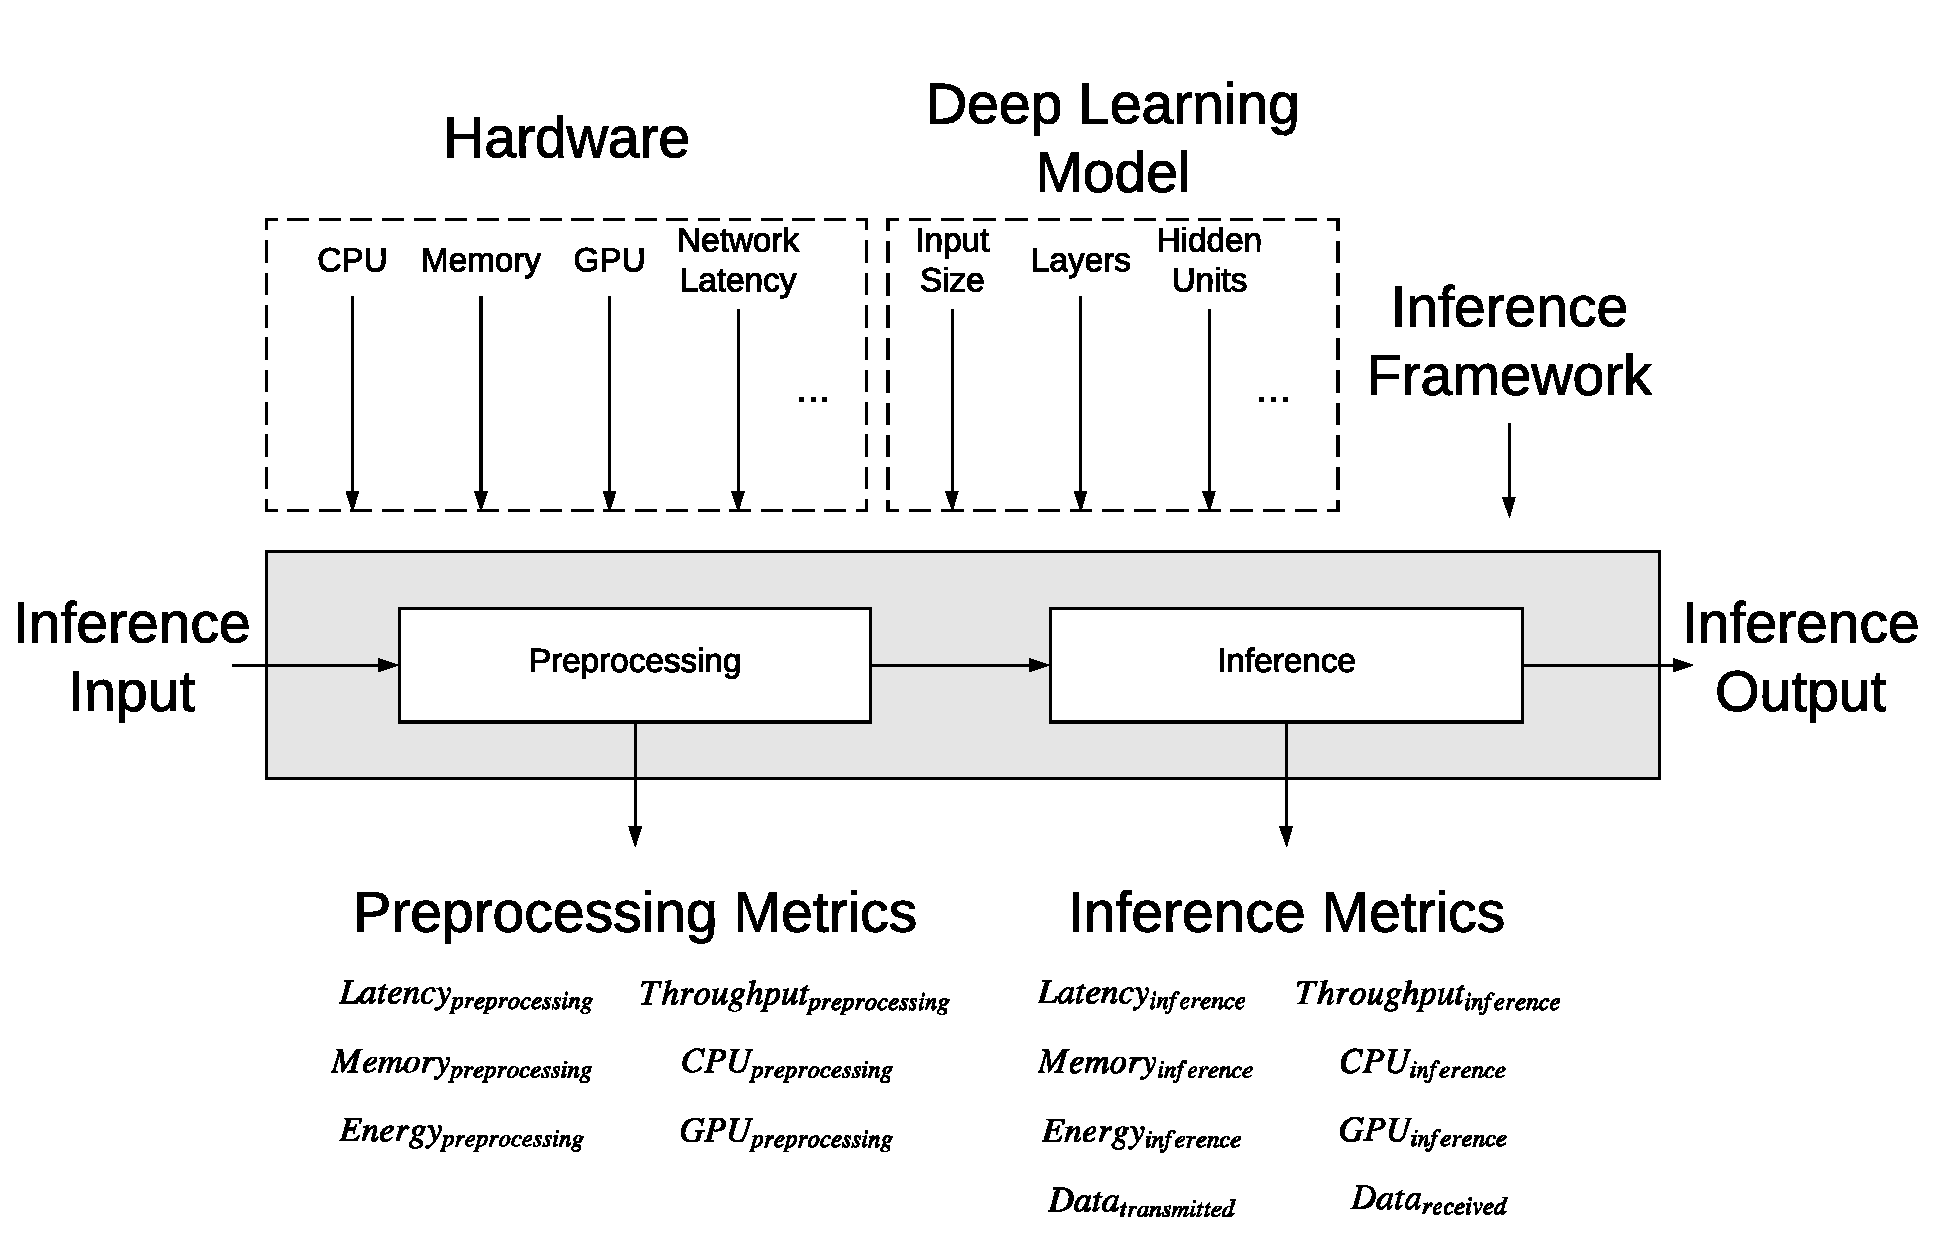
\includegraphics[width=0.99\textwidth]{./Bilder/PerformanceModel.pdf}
\caption{Problem Space with factors influencing the inference performance and the for the inference performance essential performance metrics}
\label{fig:perfmodel}
\end{figure}

To get the model output for a given inference input two steps are needed. The first one is the preprocessing step and transforms a given input into the format that is required by the deep learning model. Only then the actual inference operation can be performed to obtain the model output. Therefore the preprocessing takes a vital part in the general inference process and should be included in the performance model.

These inputs affect various performance metrics, of which inference latency and throughput are the most important ones for real-time AI applications on the edge. However, as the hardware on edge devices is limited and most of the times more than one application need to run in parallel, low usages of the other depicted metrics are vital as well.
In the following, we present performance metrics essential for the performance of real-time AI applications and the rationale behind them.







\section{Performance Metrics}
\label{chap:metrics}
Several metrics are important to measure the performance of the preprocessing and the inference steps. For most of the following metrics, we break down each metric into two sub-measurements, one for the preprocessing and the other for the inference part.

Except for data consumption, which is the only metric exclusive for cloud inference, because data is sent to a remote server, all metrics are relevant for both edge and cloud inference.
While accuracy is one of the most critical metrics for neural networks, it is only affected by the characteristics of the model and not by the deployment environment. Therefore we do not focus on accuracy in this thesis.

Note that we only measure the impact on inference/preprocessing on the resources on the edge devices, not the usage on the cloud-backend itself, as this thesis focuses on optimal selection for real-time AI applications on edge devices.
\subsubsection{Latency}
\label{chap:latency}
Latency is essential to determine the performance, since AI application often need predictions in real-time, resulting in need of low latencies.
The time needed to transform the original input to a shape fit for feeding into the deep learning model is called $Latency_{preprocessing}$.
%%WALL CLOCK TIME ADD HERE
$Latency_{inference}$ describes the time needed from requesting a prediction from a deep learning model given a specific input until getting the prediction.
The latency needed to perform both preprocessing and inference for a given input is called $Latency_{total}$.

For cloud inference, where network communication has to be done between a client (edge) and a server (cloud-backend), the network latency is an additional factor to the inference performance.
Therefore we split $Latency_{inference}$ in two sub metrics, $Latency_{network}$ and $Latency_{server}$, which together sum up to $Latency_{inference}$.
While $Latency_{server}$ denotes the time consumed by the cloud-backend to perform the inference on the given input, $Latency_{network}$ describes the time needed to send the inference input to the server and receive the prediction from the server.
\subsubsection{Throughput}
To accomplish real-time AI a certain level of throughput is essential. Therefore the number of predictions per second is a valuable metric. 
Since preprocessing is a vital part of the inference process, the throughput impact caused by preprocessed is also of interest.

Therefore we differentiate between three types of throughput: $Throughput_{preprocessing}$, $Throughput_{inference}$ and $Throughput_{total}$.
$Throughput_{total}$ is the throughput of the preprocessing and inference latencies combined.



\subsubsection{Energy Consumption}
$Energy_{preprocessing}$ and $Energy_{inference}$, which describe the amount of energy consumed during preprocessing and inference, are particularly important for mobile edge devices, since they often are powered by batteries with a limited lifespan. If the preprocessing or inference process consumes too much energy, the application using the model is not viable.


\subsubsection{CPU/GPU Usage}
Since the preprocessing/inference operations are most of the time not the only processes running on a system and other processes need to run simultaneously, the usages of CPU ($CPU_{inference}$, $CPU_{preprocessing}$) and GPU ($GPU_{inference}$, $GPU_{preprocessing}$) or other available accelerators are an important metric.
High usages would also indicate that performance would eventually be slowed down on devices with less CPU/GPU power.


\subsubsection{Memory Usage}
Similar to CPU usage, preprocessing and inference should not occupy the whole memory of the system or even demand more memory than the available memory. Therefore $Memory_{inference}$ and $Memory_{preprocessing}$ are of interest.
%\subsubsection{GPU Usage}
%If a GPU or an another accelerator is available their usage is of interest.

\subsubsection{Data Consumption}
$Data_{transmitted}$ and $Data_{received}$ are only relevant for cloud inference, as a request has to be sent to a remote server and the according response with prediction has to be sent back to the client. A high data consumption could slow down the inference latency significantly if the up- and downstream of the network connection is too slow. 

This is in particular important for the case where the input data for the model is preprocessed on the cloud, because the input data is often resized to a smaller shape during preprocessing. Therefore cloud preprocessing increases the amount of data that needs to be transmitted to the server. For slow network connections, this could result in higher inference latencies.

%%Add table here?




\section{Infrastructure}
\label{chap:infrastructure}
This section presents the infrastructure used for our benchmark framework, specifically used hardware components and inference frameworks both at the edge and cloud.
An overview of the used infrastructure can be seen in figure \ref{fig:expDesign}.

\begin{figure}[H]
\centering
\resizebox{.95\linewidth}{!}{

\tikzset{every picture/.style={line width=0.75pt}} %set default line width to 0.75pt        

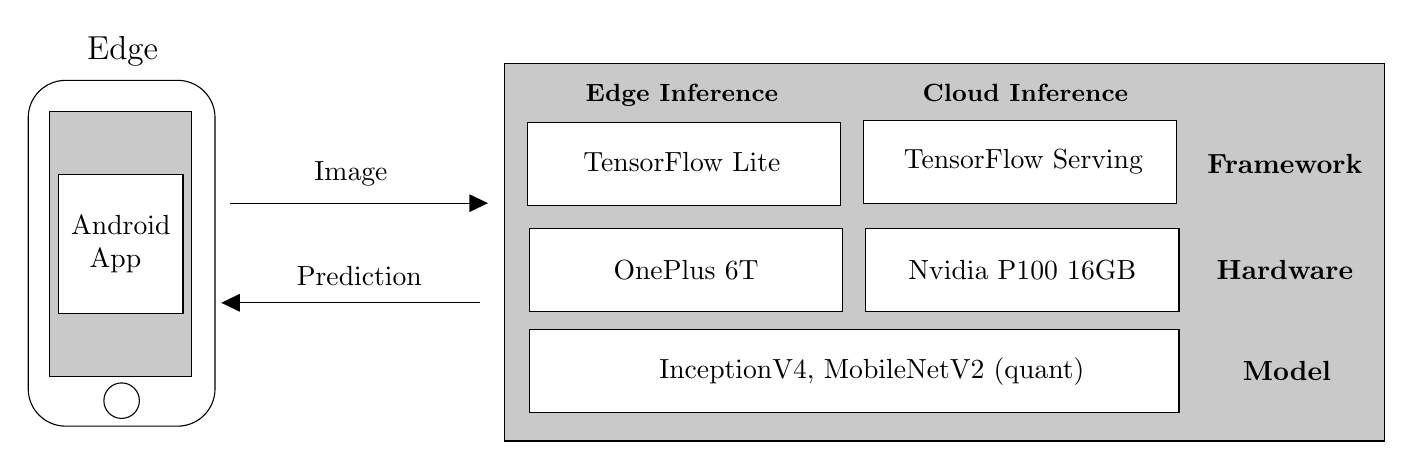
\begin{tikzpicture}[x=0.75pt,y=0.75pt,yscale=-1,xscale=1]
%uncomment if require: \path (0,485.57142639160156); %set diagram left start at 0, and has height of 485.57142639160156

%Straight Lines [id:da9993479608904674] 
\draw    (100.48,89) -- (223,89) ;
\draw [shift={(225,89)}, rotate = 540] [fill={rgb, 255:red, 0; green, 0; blue, 0 }  ][line width=0.75]  [draw opacity=0] (8.93,-4.29) -- (0,0) -- (8.93,4.29) -- cycle    ;

%Straight Lines [id:da5401559459790608] 
\draw    (98.48,137) -- (221,137) ;

\draw [shift={(96.48,137)}, rotate = 360] [fill={rgb, 255:red, 0; green, 0; blue, 0 }  ][line width=0.75]  [draw opacity=0] (8.93,-4.29) -- (0,0) -- (8.93,4.29) -- cycle    ;
%Shape: Rectangle [id:dp45054130026891115] 
\draw  [fill={rgb, 255:red, 201; green, 201; blue, 201 }  ,fill opacity=1 ] (233,21.57) -- (656.93,21.57) -- (656.93,203.57) -- (233,203.57) -- cycle ;
%Shape: Rectangle [id:dp21016153851852382] 
\draw  [fill={rgb, 255:red, 255; green, 255; blue, 255 }  ,fill opacity=1 ] (245,150) -- (557.93,150) -- (557.93,190) -- (245,190) -- cycle ;
%Shape: Rectangle [id:dp17739269402878732] 
\draw  [fill={rgb, 255:red, 255; green, 255; blue, 255 }  ,fill opacity=1 ] (244,50) -- (394.93,50) -- (394.93,90) -- (244,90) -- cycle ;
%Shape: Rectangle [id:dp9093436455970001] 
\draw  [fill={rgb, 255:red, 255; green, 255; blue, 255 }  ,fill opacity=1 ] (406,49) -- (556.93,49) -- (556.93,89) -- (406,89) -- cycle ;
%Shape: Rectangle [id:dp14120602080303146] 
\draw  [fill={rgb, 255:red, 255; green, 255; blue, 255 }  ,fill opacity=1 ] (245,101) -- (395.93,101) -- (395.93,141) -- (245,141) -- cycle ;
%Shape: Rectangle [id:dp45473714544487454] 
\draw  [fill={rgb, 255:red, 255; green, 255; blue, 255 }  ,fill opacity=1 ] (407,101) -- (557.93,101) -- (557.93,141) -- (407,141) -- cycle ;
%Shape: Rectangle [id:dp4153343207585154] 
\draw  [fill={rgb, 255:red, 201; green, 201; blue, 201 }  ,fill opacity=1 ] (13.91,44.69) -- (82.34,44.69) -- (82.34,172.63) -- (13.91,172.63) -- cycle ;
%Rounded Rect [id:dp09380596237315397] 
\draw   (3.5,47.82) .. controls (3.5,37.88) and (11.56,29.82) .. (21.5,29.82) -- (75.5,29.82) .. controls (85.44,29.82) and (93.5,37.88) .. (93.5,47.82) -- (93.5,178.43) .. controls (93.5,188.37) and (85.44,196.43) .. (75.5,196.43) -- (21.5,196.43) .. controls (11.56,196.43) and (3.5,188.37) .. (3.5,178.43) -- cycle ;
%Shape: Ellipse [id:dp8964060056788943] 
\draw   (39.95,184.16) .. controls (39.95,179.43) and (43.78,175.6) .. (48.5,175.6) .. controls (53.22,175.6) and (57.05,179.43) .. (57.05,184.16) .. controls (57.05,188.88) and (53.22,192.71) .. (48.5,192.71) .. controls (43.78,192.71) and (39.95,188.88) .. (39.95,184.16) -- cycle ;
%Shape: Rectangle [id:dp85708751067272] 
\draw  [fill={rgb, 255:red, 255; green, 255; blue, 255 }  ,fill opacity=1 ] (18.19,75.22) -- (78.07,75.22) -- (78.07,142.1) -- (18.19,142.1) -- cycle ;

% Text Node
\draw (159,75) node  [align=left] {Image};
% Text Node
\draw (163,124) node  [align=left] {Prediction};
% Text Node
\draw (49,16) node  [align=left] {{\large Edge}};
% Text Node
\draw (409.96,170) node  [align=left] {InceptionV4, MobileNetV2 (quant)};
% Text Node
\draw (318.46,37) node  [align=left] {{\small \textbf{Edge Inference}}};
% Text Node
\draw (483.96,36) node  [align=left] {{\small \textbf{Cloud Inference}}};
% Text Node
\draw (318.46,69) node  [align=left] {TensorFlow Lite};
% Text Node
\draw (482.96,68.79) node  [align=left] {TensorFlow Serving};
% Text Node
\draw (320.46,121) node  [align=left] {OnePlus 6T};
% Text Node
\draw (482.46,121) node  [align=left] {Nvidia P100 16GB};
% Text Node
\draw (608.96,70) node  [align=left] {\textbf{Framework}};
% Text Node
\draw (608.96,121) node  [align=left] {\textbf{Hardware}};
% Text Node
\draw (609.96,170) node  [align=left] {\textbf{Model}};
% Text Node
\draw (48.13,108.66) node  [align=left] {Android\\ \ \ App};


\end{tikzpicture}}
\caption{Infrastructure Overview}
\label{fig:expDesign}
\end{figure}


\subsection{Hardware}
In this thesis, we will benchmark one edge devices as well as one server, which will serve as the cloud-backend.
More devices would help illustrate the effect of different hardware environments better, but due to limited time, benchmarks for other devices are not possible.
\subsubsection{Edge}
\label{chap:hardwareEdge}
As the edge device we will use the OnePlus 6T (ONEPLUS A6013). This state of the art smartphone is powered by a Qualcomm Snapdragon 845 CPU (Octa-core, up to $2.8$ GHz), Adreno $630$ GPU, $8$ GB of memory and runs on OxygenOS $9.0.11$, which is based on Android $9$.
%%Cite from AI bechmark paper
\subsubsection{Cloud}
%The Nvidia DGX-1 will serve as the cloud-backend for the experiments. This server consists of 8$\times$Tesla V100 providing 1000 TFLOPS as well as 256 GB GPU memory and 512 GB system memory.
We use a virtual server hosted at the LRZ, which has 32 cores (16 real cores with hyperthreading), 240 GB of memory, a Tesla P100 16 GB PCIe GPGPU and a 800 PCIe SSD.
The server runs on Ubuntu 16.04 CUDA 9.1 PGI 17.9 nvidia-docker 2.0.3+docker18.03.1-1.
\subsection{Inference Framework}
We use two open source machine learning frameworks, both based on TensorFlow, for the experiments, TensorFlow Lite and TensorFlow Serving. We decided to use these frameworks, because they are open source and support, at the point of this theses, most of the operations needed for the popular image classification models as well as an increasing number of hardware accelerators and operating systems for both edge and cloud inference.
TensorFlow provides official releases of deep learning models, that are well maintained and tested, including the ones we use in this thesis.

This section only gives a brief overview of the most important aspects of the frameworks, for detailed information consider the TensorFlow Lite\cite{tfLite}  and TensorFlow Serving\cite{tfServing} websites, on which this section is partly based on, or the corresponding GitHub repositories.
\subsubsection{TensorFlow Lite}
\label{chap:TFLite}
TensorFlow Lite (Release 1.12.0) was developed for mobile and embedded devices and is a lightweight solution of TensorFlow and thus will be used for the edge inference experiments.

%%Mention NNAPI support?
At the moment only model inference can be made by TensorFlow Lite, not model training.
It supports acceleration with GPU or other accelerators as well as portability to Android, iOS and other IoT devices.

\paragraph{Android NNAPI}
\label{chap:NNAPI}
TensorFlow Lite is also compatible with the Android Neural Networks API\footnote{https://developer.android.com/ndk/guides/neuralnetworks/} (NNAPI). This API
is designed to speed up computationally intensive machine learning operations and can be used by TensorFlow Lite to improve inference performance. During inference NNAPI "can
efficiently distribute the computation workload across available on-device processors, including dedicated neural network chips, GPUs and DSPs"\cite{DBLP:journals/corr/abs-1810-01109}.

Figure \ref{fig:NNAPIarchitecture} shows the architecture of the NNAPI. In our use case the application is our android benchmark application presented in section \ref{chap:androidApp} and the machine learning framework we use is TensorFlow Lite.
\begin{figure}[!htb]
\centering
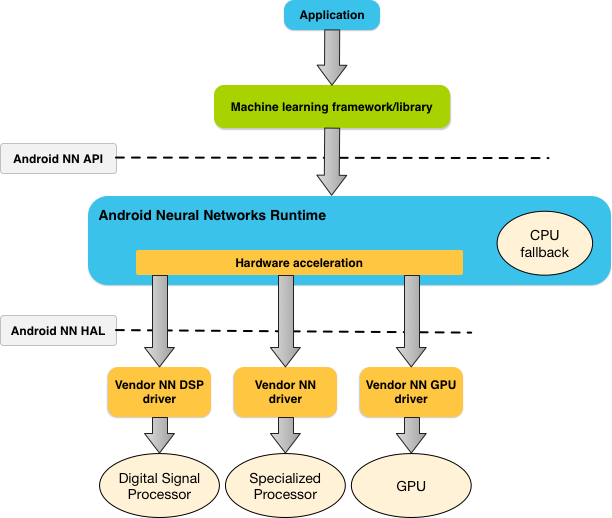
\includegraphics[width=0.5\textwidth]{./Bilder/nnapi_architecture.png}
\caption{System architecture for NNAPI framework \cite{NNAPI}}
\label{fig:NNAPIarchitecture}
\end{figure}


\paragraph{Hosting Models}
TensorFlow Lite expects models in their own \emph{FlatBuffer} file  format(\emph{.tflite}). Therefore models need to be converted to this format before TensorFlow Lite can load them. This conversion can be done using the TensorFlow Lite Converter, which supports various formats of trained TensorFlow models.
After conversion an object of the Interpreter class can load the \emph{.tflite} file.
\paragraph{Run Prediction}

To then run the inference process in TensorFlow Lite the run method of Interpreter object with a loaded model needs to be called. To call this function two objects need to be passed, first the input for the given model and second the output object, where the prediction response from the inference operation get stored. 
\begin{figure}[H]
\centering



\tikzset{every picture/.style={line width=0.75pt}} %set default line width to 0.75pt        

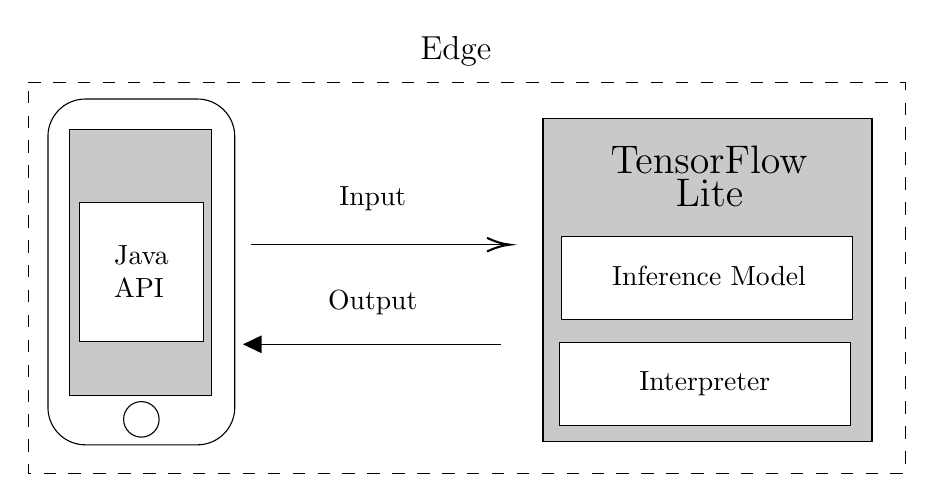
\begin{tikzpicture}[x=0.75pt,y=0.75pt,yscale=-1,xscale=1]
%uncomment if require: \path (0,300); %set diagram left start at 0, and has height of 300

%Shape: Rectangle [id:dp13292222689234756] 
\draw  [fill={rgb, 255:red, 201; green, 201; blue, 201 }  ,fill opacity=1 ] (61.91,111.69) -- (130.34,111.69) -- (130.34,239.63) -- (61.91,239.63) -- cycle ;
%Rounded Rect [id:dp7897713915001106] 
\draw   (51.5,114.82) .. controls (51.5,104.88) and (59.56,96.82) .. (69.5,96.82) -- (123.5,96.82) .. controls (133.44,96.82) and (141.5,104.88) .. (141.5,114.82) -- (141.5,245.43) .. controls (141.5,255.37) and (133.44,263.43) .. (123.5,263.43) -- (69.5,263.43) .. controls (59.56,263.43) and (51.5,255.37) .. (51.5,245.43) -- cycle ;
%Shape: Ellipse [id:dp9670901006981827] 
\draw   (87.95,251.16) .. controls (87.95,246.43) and (91.78,242.6) .. (96.5,242.6) .. controls (101.22,242.6) and (105.05,246.43) .. (105.05,251.16) .. controls (105.05,255.88) and (101.22,259.71) .. (96.5,259.71) .. controls (91.78,259.71) and (87.95,255.88) .. (87.95,251.16) -- cycle ;
%Straight Lines [id:da9993479608904674] 
\draw    (149.48,167) -- (272,167) ;
\draw [shift={(274,167)}, rotate = 540] [color={rgb, 255:red, 0; green, 0; blue, 0 }  ][line width=0.75]    (10.93,-3.29) .. controls (6.95,-1.4) and (3.31,-0.3) .. (0,0) .. controls (3.31,0.3) and (6.95,1.4) .. (10.93,3.29)   ;

%Straight Lines [id:da5401559459790608] 
\draw    (147.48,215) -- (270,215) ;

\draw [shift={(145.48,215)}, rotate = 360] [fill={rgb, 255:red, 0; green, 0; blue, 0 }  ][line width=0.75]  [draw opacity=0] (8.93,-4.29) -- (0,0) -- (8.93,4.29) -- cycle    ;
%Shape: Rectangle [id:dp45054130026891115] 
\draw  [fill={rgb, 255:red, 201; green, 201; blue, 201 }  ,fill opacity=1 ] (290,106) -- (448.5,106) -- (448.5,262) -- (290,262) -- cycle ;
%Shape: Rectangle [id:dp21016153851852382] 
\draw  [fill={rgb, 255:red, 255; green, 255; blue, 255 }  ,fill opacity=1 ] (299,163) -- (439,163) -- (439,203) -- (299,203) -- cycle ;
%Shape: Rectangle [id:dp8946256165796296] 
\draw  [fill={rgb, 255:red, 255; green, 255; blue, 255 }  ,fill opacity=1 ] (298,214) -- (438,214) -- (438,254) -- (298,254) -- cycle ;
%Shape: Rectangle [id:dp1345031923489386] 
\draw  [dash pattern={on 4.5pt off 4.5pt}] (42,89) -- (464.5,89) -- (464.5,277.4) -- (42,277.4) -- cycle ;
%Shape: Rectangle [id:dp7242946292477495] 
\draw  [fill={rgb, 255:red, 255; green, 255; blue, 255 }  ,fill opacity=1 ] (66.56,146.69) -- (126.44,146.69) -- (126.44,213.56) -- (66.56,213.56) -- cycle ;

% Text Node
\draw (208,145) node  [align=left] {Input};
% Text Node
\draw (248,74) node  [align=left] {{\large Edge}};
% Text Node
\draw (370,134) node  [align=left] {{\Large TensorFlow}\\{\Large  \ \ \ \ \ Lite}};
% Text Node
\draw (370,182) node  [align=left] {Inference Model};
% Text Node
\draw (208,195) node  [align=left] {Output};
% Text Node
\draw (368,234) node  [align=left] {Interpreter};
% Text Node
\draw (96.5,180.12) node  [align=left] {Java\\ API};


\end{tikzpicture}
\caption{Functionality of TensorFlow Lite}
\label{fig:edge}
\end{figure}

\subsubsection{TensorFlow Serving}
\label{chap:TFServing}
TensorFlow Serving (Release 1.11.1) will be used as the cloud inference framework since it provides a framework to serve machine learning models in production environments at the cloud. 



\paragraph{Hosting Models}
To host a model as a \emph{Servable} in TensorFlow Serving, a TensorFlow model needs to exported using TensorFlow's \emph{SavedModelBuilder}, resulting in a \emph{SavedModel protocol} buffer file along with the model’s variables and assets (Although TensorFlow Serving is optimized for TensorFlow models, the framework can be extended to serve other types of models).
%%Wieviel schreiben über signature, predict function etc?

Now the exported model can be loaded by an instance of Tensorflow Serving.
We use docker to start that instance, specifically nvidia-docker that allows us to run the inference operations on a GPU. For that TensorFlow Serving provides two docker images of their framework, one with CPU and the other with GPU support.

\paragraph{Run Prediction}
TensorFlow Serving supports two APIs for clients to create predictions requests: gRPC and REST. Since the gRPC protocol is supposed to deliver a better performance in the form of lower latencies and smaller payloads, we will use the gRPC API in this thesis.
Before a client can make a request to the server, a gRPC stub needs to be created in the first place, that allows us to call all methods implemented on the server. In our case, we need to call TensorFlow Serving's \emph{Predict} method to start the inference process. The method needs to be passed a \emph{PredictRequest} object, which contains among other things the input data for the model, the shape of the input and the requested model.%model signature?

After the request is sent and handled the server response by sending back a \emph{PredictResponse} object. This object holds the predictions for the given input data in the form specified by the exported model.
This request and response process can also be seen in figure \ref{fig:cloud}.

\begin{figure}[H]
\centering


\tikzset{every picture/.style={line width=0.75pt}} %set default line width to 0.75pt        

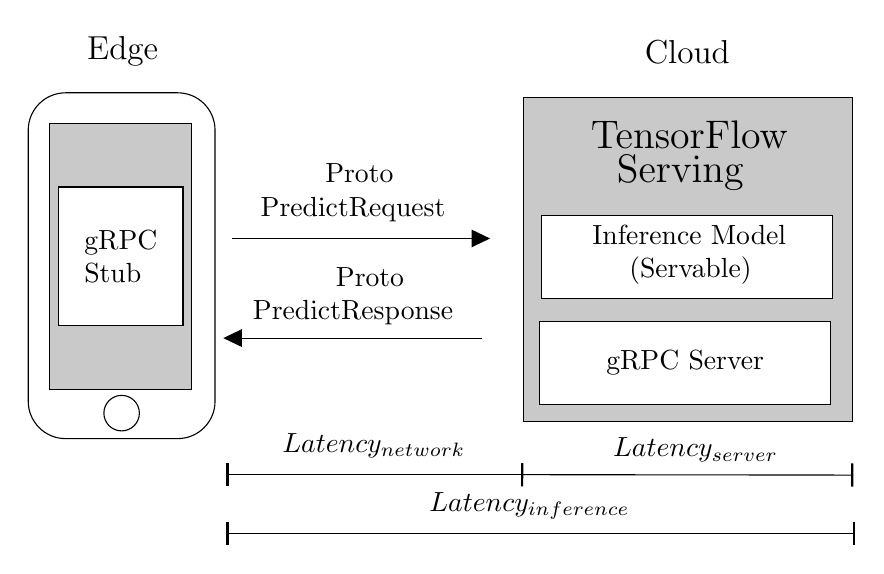
\begin{tikzpicture}[x=0.75pt,y=0.75pt,yscale=-1,xscale=1]
%uncomment if require: \path (0,300); %set diagram left start at 0, and has height of 300

%Straight Lines [id:da7072764839644827] 
\draw    (149.5,291) -- (451.5,291) ;
\draw [shift={(451.5,291)}, rotate = 180] [color={rgb, 255:red, 0; green, 0; blue, 0 }  ][line width=0.75]    (0,5.59) -- (0,-5.59)   ;
\draw [shift={(149.5,291)}, rotate = 180] [color={rgb, 255:red, 0; green, 0; blue, 0 }  ][line width=0.75]    (0,5.59) -- (0,-5.59)   ;
%Straight Lines [id:da9536138531960994] 
\draw    (291.5,262.8) -- (450.5,263) ;
\draw [shift={(450.5,263)}, rotate = 180.07] [color={rgb, 255:red, 0; green, 0; blue, 0 }  ][line width=0.75]    (0,5.59) -- (0,-5.59)   ;
\draw [shift={(291.5,262.8)}, rotate = 180.07] [color={rgb, 255:red, 0; green, 0; blue, 0 }  ][line width=0.75]    (0,5.59) -- (0,-5.59)   ;
%Shape: Rectangle [id:dp8902536871651789] 
\draw  [fill={rgb, 255:red, 201; green, 201; blue, 201 }  ,fill opacity=1 ] (63.91,93.69) -- (132.34,93.69) -- (132.34,221.63) -- (63.91,221.63) -- cycle ;
%Rounded Rect [id:dp41557214204551274] 
\draw   (53.5,96.82) .. controls (53.5,86.88) and (61.56,78.82) .. (71.5,78.82) -- (125.5,78.82) .. controls (135.44,78.82) and (143.5,86.88) .. (143.5,96.82) -- (143.5,227.43) .. controls (143.5,237.37) and (135.44,245.43) .. (125.5,245.43) -- (71.5,245.43) .. controls (61.56,245.43) and (53.5,237.37) .. (53.5,227.43) -- cycle ;
%Shape: Ellipse [id:dp8878397246816687] 
\draw   (89.95,233.16) .. controls (89.95,228.43) and (93.78,224.6) .. (98.5,224.6) .. controls (103.22,224.6) and (107.05,228.43) .. (107.05,233.16) .. controls (107.05,237.88) and (103.22,241.71) .. (98.5,241.71) .. controls (93.78,241.71) and (89.95,237.88) .. (89.95,233.16) -- cycle ;
%Straight Lines [id:da5813802620369573] 
\draw    (151.48,149) -- (274,149) ;
\draw [shift={(276,149)}, rotate = 540] [fill={rgb, 255:red, 0; green, 0; blue, 0 }  ][line width=0.75]  [draw opacity=0] (8.93,-4.29) -- (0,0) -- (8.93,4.29) -- cycle    ;

%Straight Lines [id:da16220168680973557] 
\draw    (149.48,197) -- (272,197) ;

\draw [shift={(147.48,197)}, rotate = 360] [fill={rgb, 255:red, 0; green, 0; blue, 0 }  ][line width=0.75]  [draw opacity=0] (8.93,-4.29) -- (0,0) -- (8.93,4.29) -- cycle    ;
%Shape: Rectangle [id:dp8411150472244695] 
\draw  [fill={rgb, 255:red, 201; green, 201; blue, 201 }  ,fill opacity=1 ] (292,81) -- (450.5,81) -- (450.5,237) -- (292,237) -- cycle ;
%Shape: Rectangle [id:dp13557861576626729] 
\draw  [fill={rgb, 255:red, 255; green, 255; blue, 255 }  ,fill opacity=1 ] (301,138) -- (441,138) -- (441,178) -- (301,178) -- cycle ;
%Shape: Rectangle [id:dp5681963435258506] 
\draw  [fill={rgb, 255:red, 255; green, 255; blue, 255 }  ,fill opacity=1 ] (68.19,124.22) -- (128.07,124.22) -- (128.07,191.1) -- (68.19,191.1) -- cycle ;
%Shape: Rectangle [id:dp7458124222136935] 
\draw  [fill={rgb, 255:red, 255; green, 255; blue, 255 }  ,fill opacity=1 ] (300,189) -- (440,189) -- (440,229) -- (300,229) -- cycle ;
%Straight Lines [id:da6846625455377753] 
\draw    (149.5,262.8) -- (291.5,262.8) ;
\draw [shift={(291.5,262.8)}, rotate = 180] [color={rgb, 255:red, 0; green, 0; blue, 0 }  ][line width=0.75]    (0,5.59) -- (0,-5.59)   ;
\draw [shift={(149.5,262.8)}, rotate = 180] [color={rgb, 255:red, 0; green, 0; blue, 0 }  ][line width=0.75]    (0,5.59) -- (0,-5.59)   ;

% Text Node
\draw (375,251) node  [align=left] {$\displaystyle Latency_{server}$$ $};
% Text Node
\draw (210,127) node  [align=left] { \ \ \ \ \ \ \ Proto\\PredictRequest};
% Text Node
\draw (99,59) node  [align=left] {{\large Edge}};
% Text Node
\draw (371,59) node  [align=left] {{\large Cloud}};
% Text Node
\draw (372,109) node  [align=left] {{\Large TensorFlow}\\{\Large  \ \ Serving}};
% Text Node
\draw (372,157) node  [align=left] {Inference Model\\ \ \ \ \ (Servable)};
% Text Node
\draw (210,177) node  [align=left] { \ \ \ \ \ \ \ \ \ Proto\\PredictResponse};
% Text Node
\draw (98.13,157.66) node  [align=left] {gRPC\\ Stub};
% Text Node
\draw (370,209) node  [align=left] {gRPC Server};
% Text Node
\draw (220,249) node  [align=left] {$\displaystyle Latency_{network}$$ $};
% Text Node
\draw (295,278) node  [align=left] {$\displaystyle Latency_{inference}$$ $};


\end{tikzpicture}
\caption{Basic Functionality of TensorFlow Serving}
\label{fig:cloud}
\end{figure}
 
%\section{Experimental Design}
%This section deals the specification of the Android benchmark application, used hardware, frameworks, models and how the measurements are conducted. 
%Figure \ref{fig:expDesign} depicts a brief overview of the design of the experiments, more precisely the used models, frameworks and hardware components, which are presented in greater detail in this section.
%The role of the Android benchmark application is to simulate a AI application that delegates the inputs, which in our use case are images, to the edge or cloud inference framework for the inference process and gets the predictions as a response from the frameworks.




\section{Parameters}
\label{chap:parameters}
There are two types of parameters, workload and factors.
Factors are system parameters with various levels affecting system performance, for example usage of an accelerator.
Workloads are requests to the system by a user, in our case request with a given image to a specific deep learning model, that is hosted by the system.
This requests can come in different shapes, thus having a different impact
on performance.
\subsection{Workload}
\label{chap:workload}
The methodology of this thesis will be illustrated on the use case of image classification, as state of the art image classification deep learning models are demanding in computational power as well as of high interest for real-time AI applications using these models for inference purposes.

There are two types of workload, first being the image classification model itself, as each architecture has different computational requirements.
This thesis will benchmark three different image classification models with significant differences in their architecture to illustrate their impact on inference performance.

The second type is the input data, in our use images, on which the inference should be performed.
This images come in various shapes and sizes and have to be preprocessed to the shape defined in the architecture of the image classification model.
To study the impact of these various shapes on the preprocessing step, we present different example images in this section.

\subsubsection{Image Classification Models}
\label{chap:models}
We will benchmark three different image classification models in this thesis, MobileNetV2, InceptionV4 and quantized MobileNetV2. The first is optimized for mobile deployment, the second towards high accuracy and the last one is a further optimized version of the first model.
All models are trained on the ImageNet dataset consisting of 1001 image classes (1000 image classes + 1 class for other image classes).
An overview of the models can be seen in table \ref{table:modelOverview} in the form of top-5 accuracy (a prediction is classified as accurate if the five labels with the highest confidence contain the real class of the input image), the input size of the model, the number of parameters in millions and the model size in the TensorFlow Lite format.
InceptionV4 has $4.5\%$ more accuracy than MobileNetV2, but also more than $12$ times more parameters and $7.5$ times larger TensorFlow Lite model size.
MobileNetV2 also uses a smaller input sizes of $224\times224$ than InceptionV4's $299\times299$ input size.
\begin{table}[H]
%CITE inception params ned vergessen
%http://dgschwend.github.io/netscope/#/preset/inceptionv4
\caption{Overview of used models}
\label{table:modelOverview}
\begin{tabular}{@{}lllll@{}}
\toprule
Model & Parameters & Top-5 Accuracy\cite{modelspecs} & Input Size & \emph{.tflite} Model Size \\
\midrule
InceptionV4 & $42.68$M\cite{InceptionV4params} & $95.1\%$ & $299\times299$ & $107.7$MB \\
MobileNetV2 1.0 & $3.47$M\cite{DBLP:journals/corr/abs-1801-04381} & $90.6\%$ & $224\times224$ & $14$MB \\
\begin{tabular}[c]{@{}l@{}}MobileNetV2 1.0\\quantized\end{tabular}  & $3.47$M\cite{DBLP:journals/corr/abs-1801-04381} & $89.9\%$ & $224\times224$ & $3.4$MB\\
\bottomrule
\end{tabular}
\end{table}
For TensorFlow Lite we use the models provided on the TensorFlow Lite website \cite{tfLiteModels}.
To convert model suitable for TensorFlow Serving, we use the TensorFlow-Slim library \cite{tfSlim}, where maintained and tested implementations of popular image classification models are being published. For both Serving and Lite we use the same training checkpoint to get the same weights for the graphs.

In the following, we give a brief overview of the models, their unique building blocks and the intuition behind them.
For full details please refer to \cite{DBLP:journals/corr/abs-1801-04381} and \cite{InceptionV4}.

\paragraph{MobileNetV2}
MobileNetV2 (version 1.0) is a successor of MobileNetV1 and is "specifically tailored for mobile and resource-constrained environments" \cite{DBLP:journals/corr/abs-1801-04381}. The authors achieve this by "significantly decreasing the number of operations and the memory needed while retaining the same accuracy"  \cite{DBLP:journals/corr/abs-1801-04381} and introducing a new layer module called "the
inverted residual with linear bottleneck".

This module is visualized in figure \ref{fig:bottleneckBlock} and consists of two parts: The inverted residual block and a shortcut from the input to the output.
In a first step of the inverted residual block, the channel dimensions of the input are expanded with the use of a pointwise $1\times1$ convolution layer. 
Afterwards depthwise $3\times3$ convolution is applied to the expanded input. Then again a pointwise $1\times1$ convolution gets used, but this time the dimensions are decreased instead of increased.

The intuition behind this module is that the expansion decodes information ensuring that the features can be extracted during the depthwise convolution. The extracted features then get encoded again by reducing the dimensions.
To improve the backpropagation of the gradient across multiple layers during the training the authors add the shortcut to the module, resulting in faster training and better accuracy.
The bottleneck module can be implemented very memory efficient, thus particularly fit for edge inference.

Figure \ref{fig:MobileNetArchi} displays the overall architecture of the model, with the majority of the building blocks being the bottleneck modules.
All bottleneck modules in a sequence have the same number of output channels and use a stride of $1$, except for the first bottleneck block in a sequence. All spatial convolutions use $3\times3$ kernels. 
Although not depicted on the figure, the model uses dropout and batch normalization during training.
%%expanstionf actor?
%%$$shortcut!! expanded by a "expansion factor" varying for different seqences

\begin{figure}[!htb]
\centering
   \resizebox{.7\linewidth}{!}{

\tikzset{every picture/.style={line width=0.75pt}} %set default line width to 0.75pt        

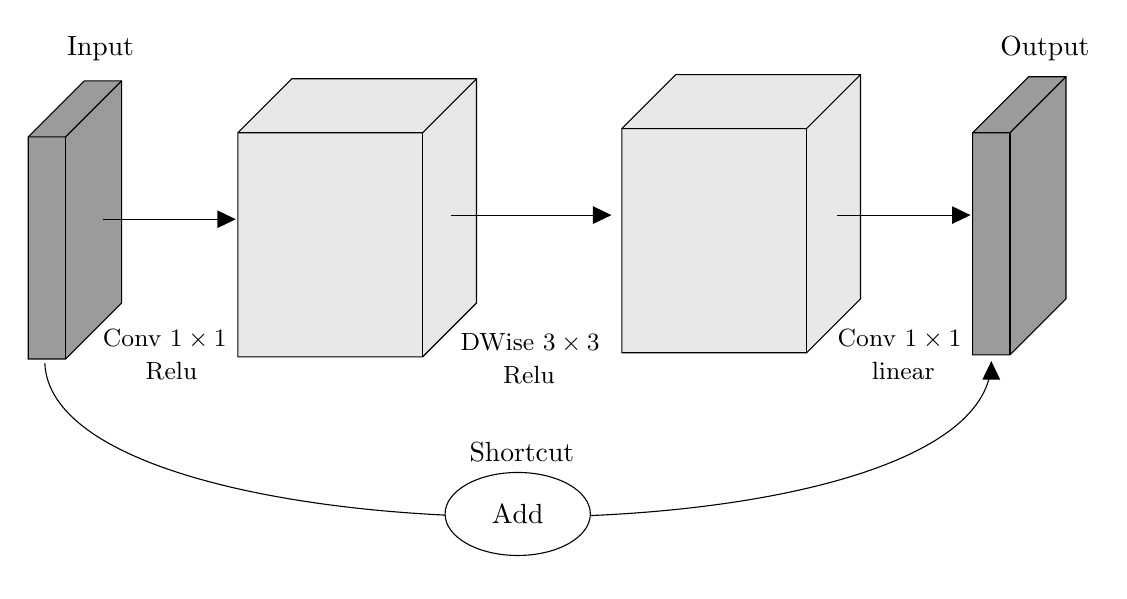
\begin{tikzpicture}[x=0.75pt,y=0.75pt,yscale=-1,xscale=1]
%uncomment if require: \path (0,600); %set diagram left start at 0, and has height of 600

%Shape: Cube [id:dp0950450187441989] 
\draw  [fill={rgb, 255:red, 155; green, 155; blue, 155 }  ,fill opacity=1 ] (24.17,60.33) -- (51.17,33.33) -- (69.17,33.33) -- (69.17,140.33) -- (42.17,167.33) -- (24.17,167.33) -- cycle ; \draw   (69.17,33.33) -- (42.17,60.33) -- (24.17,60.33) ; \draw   (42.17,60.33) -- (42.17,167.33) ;
%Shape: Cube [id:dp5388410753431343] 
\draw  [fill={rgb, 255:red, 155; green, 155; blue, 155 }  ,fill opacity=1 ] (479.17,58.33) -- (506.17,31.33) -- (524.17,31.33) -- (524.17,138.33) -- (497.17,165.33) -- (479.17,165.33) -- cycle ; \draw   (524.17,31.33) -- (497.17,58.33) -- (479.17,58.33) ; \draw   (497.17,58.33) -- (497.17,165.33) ;
%Shape: Cube [id:dp5352049268129733] 
\draw  [fill={rgb, 255:red, 232; green, 232; blue, 232 }  ,fill opacity=1 ] (125.17,58.33) -- (151.17,32.33) -- (240.17,32.33) -- (240.17,140.33) -- (214.17,166.33) -- (125.17,166.33) -- cycle ; \draw   (240.17,32.33) -- (214.17,58.33) -- (125.17,58.33) ; \draw   (214.17,58.33) -- (214.17,166.33) ;
%Shape: Cube [id:dp5972901431854747] 
\draw  [fill={rgb, 255:red, 232; green, 232; blue, 232 }  ,fill opacity=1 ] (310.17,56.33) -- (336.17,30.33) -- (425.17,30.33) -- (425.17,138.33) -- (399.17,164.33) -- (310.17,164.33) -- cycle ; \draw   (425.17,30.33) -- (399.17,56.33) -- (310.17,56.33) ; \draw   (399.17,56.33) -- (399.17,164.33) ;
%Curve Lines [id:da4213776555105224] 
\draw    (32.17,169.33) .. controls (36.15,266.84) and (483.66,269.31) .. (488.13,169.84) ;
\draw [shift={(488.17,168.33)}, rotate = 450] [fill={rgb, 255:red, 0; green, 0; blue, 0 }  ][line width=0.75]  [draw opacity=0] (8.93,-4.29) -- (0,0) -- (8.93,4.29) -- cycle    ;

%Straight Lines [id:da7525961556824932] 
\draw    (60,100) -- (122.17,100) ;
\draw [shift={(124.17,100)}, rotate = 180] [fill={rgb, 255:red, 0; green, 0; blue, 0 }  ][line width=0.75]  [draw opacity=0] (8.93,-4.29) -- (0,0) -- (8.93,4.29) -- cycle    ;

%Straight Lines [id:da7778926134720376] 
\draw    (228,98) -- (303.17,98) ;
\draw [shift={(305.17,98)}, rotate = 180] [fill={rgb, 255:red, 0; green, 0; blue, 0 }  ][line width=0.75]  [draw opacity=0] (8.93,-4.29) -- (0,0) -- (8.93,4.29) -- cycle    ;

%Straight Lines [id:da2814517292192529] 
\draw    (414,98) -- (476.17,98) ;
\draw [shift={(478.17,98)}, rotate = 180] [fill={rgb, 255:red, 0; green, 0; blue, 0 }  ][line width=0.75]  [draw opacity=0] (8.93,-4.29) -- (0,0) -- (8.93,4.29) -- cycle    ;

%Shape: Ellipse [id:dp8668947513316778] 
\draw  [fill={rgb, 255:red, 255; green, 255; blue, 255 }  ,fill opacity=1 ] (225,242) .. controls (225,230.95) and (240.67,222) .. (260,222) .. controls (279.33,222) and (295,230.95) .. (295,242) .. controls (295,253.05) and (279.33,262) .. (260,262) .. controls (240.67,262) and (225,253.05) .. (225,242) -- cycle ;

% Text Node
\draw (262,212) node  [align=left] {Shortcut};
% Text Node
\draw (90,165) node  [align=left] {{\small Conv $\displaystyle 1\times 1$}\\{\small  \ \ \ \ \ Relu}};
% Text Node
\draw (266,167) node  [align=left] {{\small DWise $\displaystyle 3\times 3$}\\{\small  \ \ \ \ \ Relu}};
% Text Node
\draw (444,165) node  [align=left] {{\small Conv $\displaystyle 1\times 1$}\\{\small  \ \ \ \ linear}};
% Text Node
\draw (260,242) node  [align=left] {Add};
% Text Node
\draw (59,18) node  [align=left] {Input};
% Text Node
\draw (514,18) node  [align=left] {Output};


\end{tikzpicture}}
\caption{Inverted Residual Block (bottleneck)}
\label{fig:bottleneckBlock}
%%NO DROPOUT AT INFERENCE
\end{figure}


\begin{comment}


\begin{table}[]

\centering
\caption{MobilenetV2 architecture \cite{DBLP:journals/corr/abs-1801-04381}}
\label{table:mobilenetArchi}
\begin{tabular}{@{}llllll@{}}

\toprule
Input & Operator & t & c & n & s \\ \midrule
$224^2\times 3$ & conv2d & - & 32 & 1 & 2 \\
$112^2\times 32$ & bottleneck & 1 & 16 & 1 & 1 \\
$112^2\times 16$ & bottleneck & 6 & 24 & 2 & 2 \\
$56^2\times 24$ & bottleneck & 6 & 32 & 3 & 2 \\
$28^2\times 23$ & bottleneck & 6 & 64 & 4 & 2 \\
$14^2\times 64$ & bottleneck & 6 & 96 & 3 & 1 \\
$14^2\times 96$ & bottleneck & 6 & 160 & 3 & 2 \\
$7^2\times 160$ & bottleneck & 6 & 320 & 1 & 1 \\
$7^2\times 320$ & conv2d 1x1 & - & 1280 & 1 & 1 \\
$7^2\times 1280$ & avgpool 7x7 & - & - & 1 & - \\
$1\times 1\times 1280$ & conv2d 1x1 & - & k & - &  \\ \bottomrule
\end{tabular}
\end{table}
\end{comment}
\subparagraph{Quantization}
Quantization of MobileNetV2, using the techniques presented in section \ref{chap:quant}, results in a  0.7\% loss of top-5 accuracy, but therefore has lost 75\% of its model size (see table \ref{table:modelOverview}) and is supposed to deliver a better inference performance, which we will evaluate in the benchmarks.



\paragraph{Inception V4}
%%Add infos about stem and reduction
InceptionV4, published in \cite{InceptionV4}, is a large image classification network with high accuracy, but also with a high number of parameters leading to higher computational demands than MobileNetV2 and thus larger impact on inference performance.
In comparison to its previous versions, InceptionV4 is built with "a more uniform simplified architecture and more inception modules"\cite{InceptionV4}. 

The general architecture of the network can be seen in figure \ref{fig:inceptionv4Archi} with the fundamental building blocks being multiple Inception (A-C) and Reduction(A-B) modules. 
An example for both of these modules can be seen in figures \ref{fig:InceptionA} and \ref{fig:InceptionReduction}.
Inception modules are built of multiple convolutions with multiple filters and pooling layers in parallel within the same layer.
After the convolutions, the output of all convolutions is concatenated.
The intuition behind this parallelism is to give the model multiple convolution choices for a given input and let the model learn itself the best feature extractor. An additional benefit is that the model can extract both local and more complex feature from an input.

To reduce the dimensionality before computational expensive large convolutions, and thus speed up training, the authors introduce the Reduction block containing small $1\times1$ convolutions.   %genauer erklären




\begin{figure}[!htb]
\centering
\begin{subfigure}[b]{.95\textwidth}
\centering
   \resizebox{.8\linewidth}{!}{

\tikzset{every picture/.style={line width=0.75pt}} %set default line width to 0.75pt        

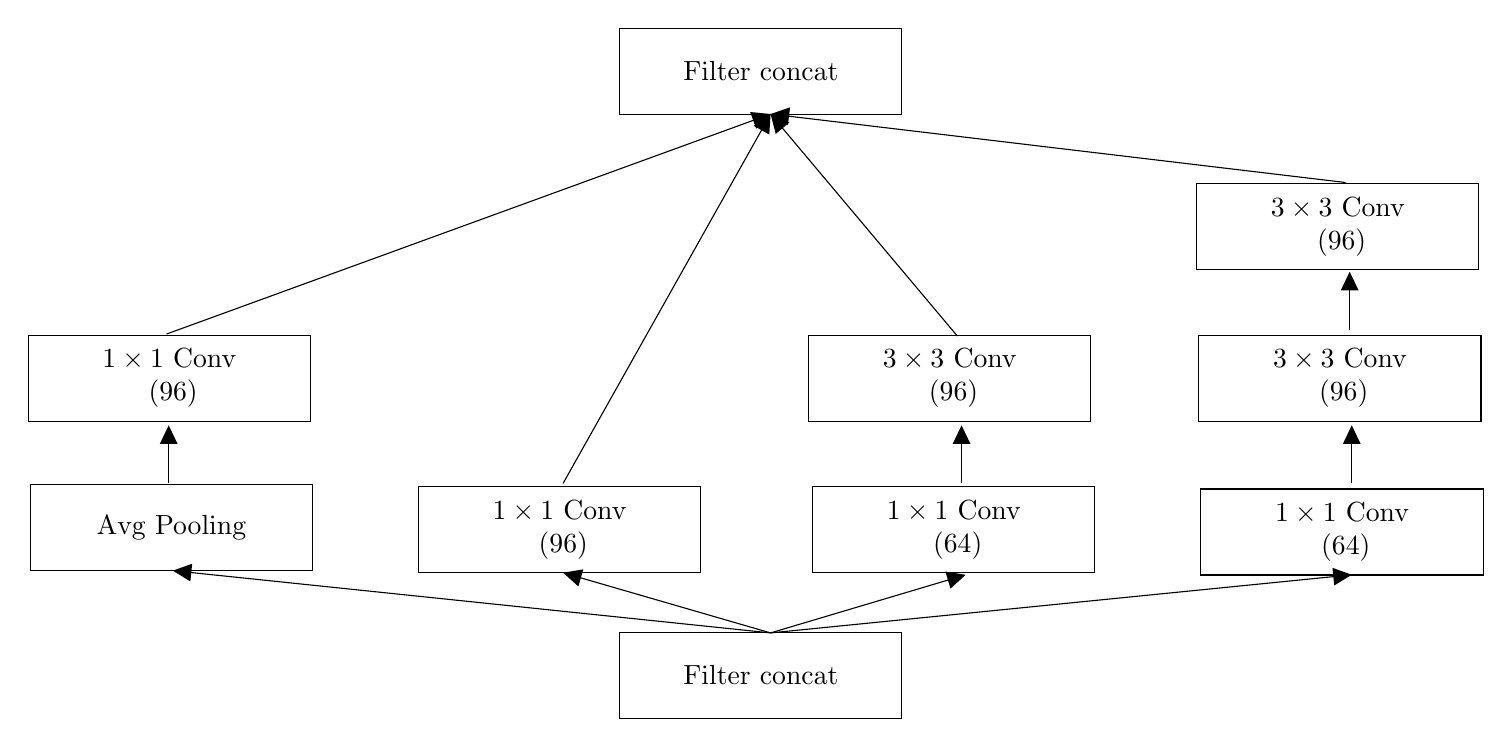
\begin{tikzpicture}[x=0.75pt,y=0.75pt,yscale=-1,xscale=1]
%uncomment if require: \path (0,550.3333358764648); %set diagram left start at 0, and has height of 550.3333358764648

%Flowchart: Process [id:dp8446713243434529] 
\draw   (508,479) -- (643.93,479) -- (643.93,520.43) -- (508,520.43) -- cycle ;
%Flowchart: Process [id:dp8389212433494444] 
\draw   (224,408) -- (359.93,408) -- (359.93,449.43) -- (224,449.43) -- cycle ;
%Flowchart: Process [id:dp9696039225192121] 
\draw   (411,409) -- (546.93,409) -- (546.93,450.43) -- (411,450.43) -- cycle ;
%Flowchart: Process [id:dp31126408548780393] 
\draw   (601,409) -- (736.93,409) -- (736.93,450.43) -- (601,450.43) -- cycle ;
%Flowchart: Process [id:dp739948518816423] 
\draw   (788,410) -- (923.93,410) -- (923.93,451.43) -- (788,451.43) -- cycle ;
%Straight Lines [id:da20227844614554824] 
\draw    (580.67,479.33) -- (294.66,449.54) ;
\draw [shift={(292.67,449.33)}, rotate = 365.95] [fill={rgb, 255:red, 0; green, 0; blue, 0 }  ][line width=0.75]  [draw opacity=0] (8.93,-4.29) -- (0,0) -- (8.93,4.29) -- cycle    ;

%Straight Lines [id:da9079516459586603] 
\draw    (580.67,479.33) -- (482.59,450.89) ;
\draw [shift={(480.67,450.33)}, rotate = 376.16999999999996] [fill={rgb, 255:red, 0; green, 0; blue, 0 }  ][line width=0.75]  [draw opacity=0] (8.93,-4.29) -- (0,0) -- (8.93,4.29) -- cycle    ;

%Straight Lines [id:da7697048902828942] 
\draw    (580.67,479.33) -- (672.75,451.9) ;
\draw [shift={(674.67,451.33)}, rotate = 523.4100000000001] [fill={rgb, 255:red, 0; green, 0; blue, 0 }  ][line width=0.75]  [draw opacity=0] (8.93,-4.29) -- (0,0) -- (8.93,4.29) -- cycle    ;

%Straight Lines [id:da004295071242706339] 
\draw    (580.67,479.33) -- (858.68,451.53) ;
\draw [shift={(860.67,451.33)}, rotate = 534.29] [fill={rgb, 255:red, 0; green, 0; blue, 0 }  ][line width=0.75]  [draw opacity=0] (8.93,-4.29) -- (0,0) -- (8.93,4.29) -- cycle    ;

%Flowchart: Process [id:dp6126721254059377] 
\draw   (223,336) -- (358.93,336) -- (358.93,377.43) -- (223,377.43) -- cycle ;
%Flowchart: Process [id:dp6415327260036892] 
\draw   (599,336) -- (734.93,336) -- (734.93,377.43) -- (599,377.43) -- cycle ;
%Flowchart: Process [id:dp557242506777897] 
\draw   (787,336) -- (922.93,336) -- (922.93,377.43) -- (787,377.43) -- cycle ;
%Flowchart: Process [id:dp895045490145193] 
\draw   (786,263) -- (921.93,263) -- (921.93,304.43) -- (786,304.43) -- cycle ;
%Straight Lines [id:da042686267300120706] 
\draw    (290.67,407.33) -- (290.67,381.33) ;
\draw [shift={(290.67,379.33)}, rotate = 450] [fill={rgb, 255:red, 0; green, 0; blue, 0 }  ][line width=0.75]  [draw opacity=0] (8.93,-4.29) -- (0,0) -- (8.93,4.29) -- cycle    ;

%Straight Lines [id:da1451751743173857] 
\draw    (672.67,407.33) -- (672.67,381.33) ;
\draw [shift={(672.67,379.33)}, rotate = 450] [fill={rgb, 255:red, 0; green, 0; blue, 0 }  ][line width=0.75]  [draw opacity=0] (8.93,-4.29) -- (0,0) -- (8.93,4.29) -- cycle    ;

%Straight Lines [id:da7065201039263691] 
\draw    (860.67,407.33) -- (860.67,381.33) ;
\draw [shift={(860.67,379.33)}, rotate = 450] [fill={rgb, 255:red, 0; green, 0; blue, 0 }  ][line width=0.75]  [draw opacity=0] (8.93,-4.29) -- (0,0) -- (8.93,4.29) -- cycle    ;

%Straight Lines [id:da3529249322466719] 
\draw    (859.67,333.33) -- (859.67,307.33) ;
\draw [shift={(859.67,305.33)}, rotate = 450] [fill={rgb, 255:red, 0; green, 0; blue, 0 }  ][line width=0.75]  [draw opacity=0] (8.93,-4.29) -- (0,0) -- (8.93,4.29) -- cycle    ;

%Flowchart: Process [id:dp023795399666625805] 
\draw   (508,188) -- (643.93,188) -- (643.93,229.43) -- (508,229.43) -- cycle ;
%Straight Lines [id:da14696140485542641] 
\draw    (289.67,335.33) -- (578.79,230.02) ;
\draw [shift={(580.67,229.33)}, rotate = 519.99] [fill={rgb, 255:red, 0; green, 0; blue, 0 }  ][line width=0.75]  [draw opacity=0] (8.93,-4.29) -- (0,0) -- (8.93,4.29) -- cycle    ;

%Straight Lines [id:da7335126004687851] 
\draw    (480.67,407.33) -- (579.69,231.08) ;
\draw [shift={(580.67,229.33)}, rotate = 479.33] [fill={rgb, 255:red, 0; green, 0; blue, 0 }  ][line width=0.75]  [draw opacity=0] (8.93,-4.29) -- (0,0) -- (8.93,4.29) -- cycle    ;

%Straight Lines [id:da6191146997492387] 
\draw    (670.67,336.33) -- (581.95,230.86) ;
\draw [shift={(580.67,229.33)}, rotate = 409.93] [fill={rgb, 255:red, 0; green, 0; blue, 0 }  ][line width=0.75]  [draw opacity=0] (8.93,-4.29) -- (0,0) -- (8.93,4.29) -- cycle    ;

%Straight Lines [id:da444168686885831] 
\draw    (857.67,262.33) -- (582.65,229.57) ;
\draw [shift={(580.67,229.33)}, rotate = 366.78999999999996] [fill={rgb, 255:red, 0; green, 0; blue, 0 }  ][line width=0.75]  [draw opacity=0] (8.93,-4.29) -- (0,0) -- (8.93,4.29) -- cycle    ;


% Text Node
\draw (575.96,499.71) node  [align=left] {Filter concat};
% Text Node
\draw (291.96,428.71) node  [align=left] {Avg Pooling};
% Text Node
\draw (478.96,429.71) node  [align=left] {$\displaystyle 1\times 1$ Conv\\ \ \ \ \ \ (96)};
% Text Node
\draw (668.96,429.71) node  [align=left] {$\displaystyle 1\times 1$ Conv\\ \ \ \ \ \ (64)};
% Text Node
\draw (855.96,430.71) node  [align=left] {$\displaystyle 1\times 1$ Conv\\ \ \ \ \ \ (64)};
% Text Node
\draw (290.96,356.71) node  [align=left] {$\displaystyle 1\times 1$ Conv\\ \ \ \ \ \ (96)};
% Text Node
\draw (666.96,356.71) node  [align=left] {$\displaystyle 3\times 3$ Conv\\ \ \ \ \ \ (96)};
% Text Node
\draw (854.96,356.71) node  [align=left] {$\displaystyle 3\times 3$ Conv\\ \ \ \ \ \ (96)};
% Text Node
\draw (853.96,283.71) node  [align=left] {$\displaystyle 3\times 3$ Conv\\ \ \ \ \ \ (96)};
% Text Node
\draw (575.96,208.71) node  [align=left] {Filter concat};


\end{tikzpicture}}
   \caption{Inception-A module}
   \label{fig:InceptionA} 
\end{subfigure}

\vspace{1em}
\begin{subfigure}[b]{.95\textwidth}
\centering
   %%Verify the architectures again
   \resizebox{.6\linewidth}{!}{

\tikzset{every picture/.style={line width=0.75pt}} %set default line width to 0.75pt        

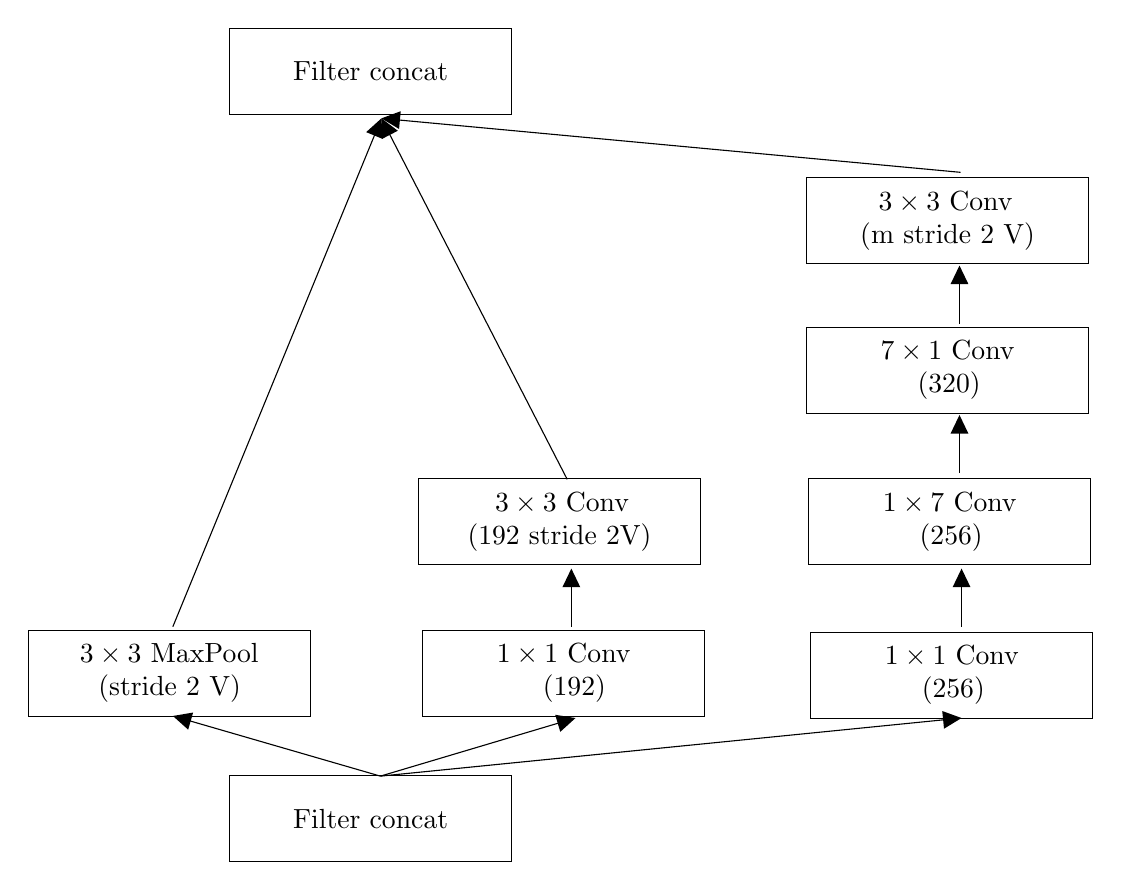
\begin{tikzpicture}[x=0.75pt,y=0.75pt,yscale=-1,xscale=1]
%uncomment if require: \path (0,470.3333282470703); %set diagram left start at 0, and has height of 470.3333282470703

%Flowchart: Process [id:dp24078826379297702] 
\draw   (528,418.9) -- (663.93,418.9) -- (663.93,460.33) -- (528,460.33) -- cycle ;
%Flowchart: Process [id:dp22165017848855517] 
\draw   (431,348.9) -- (566.93,348.9) -- (566.93,390.33) -- (431,390.33) -- cycle ;
%Flowchart: Process [id:dp6597264859137688] 
\draw   (621,348.9) -- (756.93,348.9) -- (756.93,390.33) -- (621,390.33) -- cycle ;
%Flowchart: Process [id:dp3799233367302206] 
\draw   (808,349.9) -- (943.93,349.9) -- (943.93,391.33) -- (808,391.33) -- cycle ;
%Straight Lines [id:da4490839848046586] 
\draw    (600.67,419.24) -- (502.59,390.8) ;
\draw [shift={(500.67,390.24)}, rotate = 376.16999999999996] [fill={rgb, 255:red, 0; green, 0; blue, 0 }  ][line width=0.75]  [draw opacity=0] (8.93,-4.29) -- (0,0) -- (8.93,4.29) -- cycle    ;

%Straight Lines [id:da38737183977033096] 
\draw    (600.67,419.24) -- (692.75,391.81) ;
\draw [shift={(694.67,391.24)}, rotate = 523.4100000000001] [fill={rgb, 255:red, 0; green, 0; blue, 0 }  ][line width=0.75]  [draw opacity=0] (8.93,-4.29) -- (0,0) -- (8.93,4.29) -- cycle    ;

%Straight Lines [id:da40057235552744497] 
\draw    (600.67,419.24) -- (878.68,391.44) ;
\draw [shift={(880.67,391.24)}, rotate = 534.29] [fill={rgb, 255:red, 0; green, 0; blue, 0 }  ][line width=0.75]  [draw opacity=0] (8.93,-4.29) -- (0,0) -- (8.93,4.29) -- cycle    ;

%Flowchart: Process [id:dp42511218119703864] 
\draw   (619,275.9) -- (754.93,275.9) -- (754.93,317.33) -- (619,317.33) -- cycle ;
%Flowchart: Process [id:dp6580432352234802] 
\draw   (807,275.9) -- (942.93,275.9) -- (942.93,317.33) -- (807,317.33) -- cycle ;
%Flowchart: Process [id:dp8669834254894924] 
\draw   (806,202.9) -- (941.93,202.9) -- (941.93,244.33) -- (806,244.33) -- cycle ;
%Straight Lines [id:da7396787751036953] 
\draw    (692.67,347.24) -- (692.67,321.24) ;
\draw [shift={(692.67,319.24)}, rotate = 450] [fill={rgb, 255:red, 0; green, 0; blue, 0 }  ][line width=0.75]  [draw opacity=0] (8.93,-4.29) -- (0,0) -- (8.93,4.29) -- cycle    ;

%Straight Lines [id:da2216611723462627] 
\draw    (880.67,347.24) -- (880.67,321.24) ;
\draw [shift={(880.67,319.24)}, rotate = 450] [fill={rgb, 255:red, 0; green, 0; blue, 0 }  ][line width=0.75]  [draw opacity=0] (8.93,-4.29) -- (0,0) -- (8.93,4.29) -- cycle    ;

%Straight Lines [id:da7609415385669374] 
\draw    (879.67,273.24) -- (879.67,247.24) ;
\draw [shift={(879.67,245.24)}, rotate = 450] [fill={rgb, 255:red, 0; green, 0; blue, 0 }  ][line width=0.75]  [draw opacity=0] (8.93,-4.29) -- (0,0) -- (8.93,4.29) -- cycle    ;

%Flowchart: Process [id:dp1491076780226832] 
\draw   (528,58.9) -- (663.93,58.9) -- (663.93,100.33) -- (528,100.33) -- cycle ;
%Straight Lines [id:da30781560796019103] 
\draw    (500.67,347.24) -- (600.41,104.18) ;
\draw [shift={(601.17,102.33)}, rotate = 472.31] [fill={rgb, 255:red, 0; green, 0; blue, 0 }  ][line width=0.75]  [draw opacity=0] (8.93,-4.29) -- (0,0) -- (8.93,4.29) -- cycle    ;

%Straight Lines [id:da24908463720618457] 
\draw    (690.67,276.24) -- (602.08,104.11) ;
\draw [shift={(601.17,102.33)}, rotate = 422.77] [fill={rgb, 255:red, 0; green, 0; blue, 0 }  ][line width=0.75]  [draw opacity=0] (8.93,-4.29) -- (0,0) -- (8.93,4.29) -- cycle    ;

%Flowchart: Process [id:dp01199680277761872] 
\draw   (806,130.9) -- (941.93,130.9) -- (941.93,172.33) -- (806,172.33) -- cycle ;
%Straight Lines [id:da3952124421996095] 
\draw    (879.67,201.24) -- (879.67,175.24) ;
\draw [shift={(879.67,173.24)}, rotate = 450] [fill={rgb, 255:red, 0; green, 0; blue, 0 }  ][line width=0.75]  [draw opacity=0] (8.93,-4.29) -- (0,0) -- (8.93,4.29) -- cycle    ;

%Straight Lines [id:da25220885973901197] 
\draw    (880.17,128.33) -- (603.16,102.52) ;
\draw [shift={(601.17,102.33)}, rotate = 365.32] [fill={rgb, 255:red, 0; green, 0; blue, 0 }  ][line width=0.75]  [draw opacity=0] (8.93,-4.29) -- (0,0) -- (8.93,4.29) -- cycle    ;


% Text Node
\draw (595.96,439.62) node  [align=left] {Filter concat};
% Text Node
\draw (498.96,369.62) node  [align=left] {$\displaystyle 3\times 3$ MaxPool\\ \ \ (stride $\displaystyle 2$ V)};
% Text Node
\draw (688.96,369.62) node  [align=left] {$\displaystyle 1\times 1$ Conv\\ \ \ \ \ \ ($\displaystyle 192$)};
% Text Node
\draw (875.96,370.62) node  [align=left] {$\displaystyle 1\times 1$ Conv\\ \ \ \ \ ($\displaystyle 256$)};
% Text Node
\draw (686.96,296.62) node  [align=left] {$\displaystyle \ \ \ 3\times 3$ Conv\\($\displaystyle 192$ stride $\displaystyle 2$V)};
% Text Node
\draw (874.96,296.62) node  [align=left] {$\displaystyle 1\times 7$ Conv\\ \ \ \ \ ($\displaystyle 256$)};
% Text Node
\draw (873.96,223.62) node  [align=left] {$\displaystyle 7\times 1$ Conv\\ \ \ \ \ ($\displaystyle 320$)};
% Text Node
\draw (595.96,79.62) node  [align=left] {Filter concat};
% Text Node
\draw (873.96,151.62) node  [align=left] {$\displaystyle \ \ 3\times 3$ Conv\\(m stride $\displaystyle 2$ V)};


\end{tikzpicture}}
   \caption{Reduction module (convolutions with "V" are valid, rest is same padded)}
   \label{fig:InceptionReduction}
\end{subfigure}

\caption{Special modules used by InceptionV4}

\end{figure}




Besides dropout InceptionV4 also benefits from the use of batch normalization during training.
%\begin{figure}[]
%\centering
%\resizebox{.45\linewidth}{!}{

\tikzset{every picture/.style={line width=0.75pt}} %set default line width to 0.75pt        

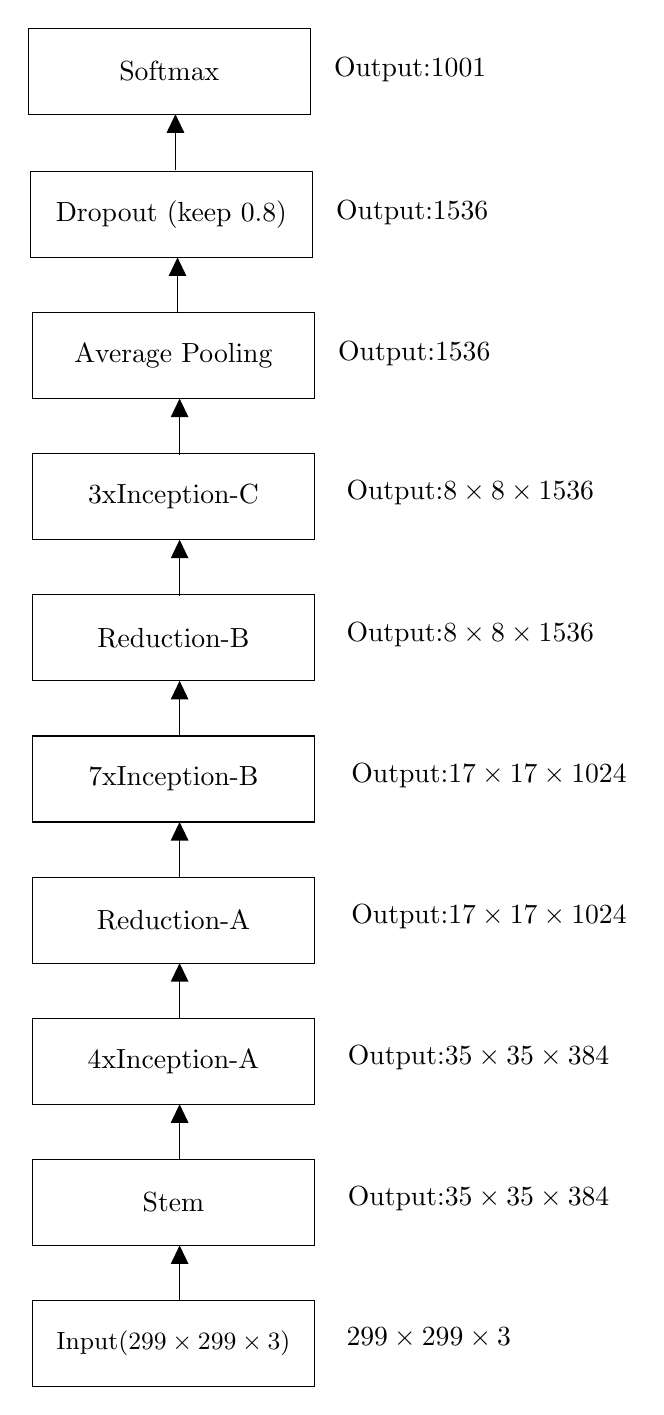
\begin{tikzpicture}[x=0.75pt,y=0.75pt,yscale=-1,xscale=1]
%uncomment if require: \path (0,742.7142868041992); %set diagram left start at 0, and has height of 742.7142868041992

%Flowchart: Process [id:dp9253173394290999] 
\draw   (98,621) -- (233.93,621) -- (233.93,662.43) -- (98,662.43) -- cycle ;
%Flowchart: Process [id:dp47578347996398307] 
\draw   (98,553) -- (233.93,553) -- (233.93,594.43) -- (98,594.43) -- cycle ;
%Straight Lines [id:da2925025767777827] 
\draw    (168.93,621.43) -- (168.93,596.43) ;
\draw [shift={(168.93,594.43)}, rotate = 450] [fill={rgb, 255:red, 0; green, 0; blue, 0 }  ][line width=0.75]  [draw opacity=0] (8.93,-4.29) -- (0,0) -- (8.93,4.29) -- cycle    ;

%Flowchart: Process [id:dp5382364848384393] 
\draw   (98,485) -- (233.93,485) -- (233.93,526.43) -- (98,526.43) -- cycle ;
%Straight Lines [id:da06940381159807729] 
\draw    (168.93,553.43) -- (168.93,528.43) ;
\draw [shift={(168.93,526.43)}, rotate = 450] [fill={rgb, 255:red, 0; green, 0; blue, 0 }  ][line width=0.75]  [draw opacity=0] (8.93,-4.29) -- (0,0) -- (8.93,4.29) -- cycle    ;

%Flowchart: Process [id:dp21301144435418706] 
\draw   (98,417) -- (233.93,417) -- (233.93,458.43) -- (98,458.43) -- cycle ;
%Straight Lines [id:da45627711718103714] 
\draw    (168.93,485.43) -- (168.93,460.43) ;
\draw [shift={(168.93,458.43)}, rotate = 450] [fill={rgb, 255:red, 0; green, 0; blue, 0 }  ][line width=0.75]  [draw opacity=0] (8.93,-4.29) -- (0,0) -- (8.93,4.29) -- cycle    ;

%Flowchart: Process [id:dp7231968775803179] 
\draw   (98,349) -- (233.93,349) -- (233.93,390.43) -- (98,390.43) -- cycle ;
%Straight Lines [id:da7165121439179447] 
\draw    (168.93,417.43) -- (168.93,392.43) ;
\draw [shift={(168.93,390.43)}, rotate = 450] [fill={rgb, 255:red, 0; green, 0; blue, 0 }  ][line width=0.75]  [draw opacity=0] (8.93,-4.29) -- (0,0) -- (8.93,4.29) -- cycle    ;

%Flowchart: Process [id:dp20620702942862734] 
\draw   (98,281) -- (233.93,281) -- (233.93,322.43) -- (98,322.43) -- cycle ;
%Straight Lines [id:da10564528480224444] 
\draw    (168.93,349.43) -- (168.93,324.43) ;
\draw [shift={(168.93,322.43)}, rotate = 450] [fill={rgb, 255:red, 0; green, 0; blue, 0 }  ][line width=0.75]  [draw opacity=0] (8.93,-4.29) -- (0,0) -- (8.93,4.29) -- cycle    ;

%Flowchart: Process [id:dp6409642010028676] 
\draw   (98,213) -- (233.93,213) -- (233.93,254.43) -- (98,254.43) -- cycle ;
%Straight Lines [id:da583110185704452] 
\draw    (168.93,281.43) -- (168.93,256.43) ;
\draw [shift={(168.93,254.43)}, rotate = 450] [fill={rgb, 255:red, 0; green, 0; blue, 0 }  ][line width=0.75]  [draw opacity=0] (8.93,-4.29) -- (0,0) -- (8.93,4.29) -- cycle    ;

%Flowchart: Process [id:dp747253235525678] 
\draw   (98,145) -- (233.93,145) -- (233.93,186.43) -- (98,186.43) -- cycle ;
%Straight Lines [id:da9482962038382927] 
\draw    (168.93,213.43) -- (168.93,188.43) ;
\draw [shift={(168.93,186.43)}, rotate = 450] [fill={rgb, 255:red, 0; green, 0; blue, 0 }  ][line width=0.75]  [draw opacity=0] (8.93,-4.29) -- (0,0) -- (8.93,4.29) -- cycle    ;

%Flowchart: Process [id:dp47103409298757426] 
\draw   (97,77) -- (232.93,77) -- (232.93,118.43) -- (97,118.43) -- cycle ;
%Straight Lines [id:da30249651940608824] 
\draw    (167.93,145.43) -- (167.93,120.43) ;
\draw [shift={(167.93,118.43)}, rotate = 450] [fill={rgb, 255:red, 0; green, 0; blue, 0 }  ][line width=0.75]  [draw opacity=0] (8.93,-4.29) -- (0,0) -- (8.93,4.29) -- cycle    ;

%Flowchart: Process [id:dp5661311837160838] 
\draw   (96,8) -- (231.93,8) -- (231.93,49.43) -- (96,49.43) -- cycle ;
%Straight Lines [id:da5142446239913938] 
\draw    (166.93,76.43) -- (166.93,51.43) ;
\draw [shift={(166.93,49.43)}, rotate = 450] [fill={rgb, 255:red, 0; green, 0; blue, 0 }  ][line width=0.75]  [draw opacity=0] (8.93,-4.29) -- (0,0) -- (8.93,4.29) -- cycle    ;


% Text Node
\draw (165.96,641.71) node  [align=left] {{\small Input($\displaystyle 299\times 299\times 3$)}};
% Text Node
\draw (165.96,573.71) node  [align=left] {Stem};
% Text Node
\draw (289,639) node  [align=left] {$\displaystyle 299\times 299\times 3$};
% Text Node
\draw (313,572) node  [align=left] {Output:$\displaystyle 35\times 35\times 384$};
% Text Node
\draw (165.96,505.71) node  [align=left] {4xInception-A};
% Text Node
\draw (313,504) node  [align=left] {Output:$\displaystyle 35\times 35\times 384$};
% Text Node
\draw (165.96,437.71) node  [align=left] {Reduction-A};
% Text Node
\draw (318,436) node  [align=left] {Output:$\displaystyle 17\times 17\times 1024$};
% Text Node
\draw (165.96,369.71) node  [align=left] {7xInception-B};
% Text Node
\draw (318,368) node  [align=left] {Output:$\displaystyle 17\times 17\times 1024$};
% Text Node
\draw (165.96,301.71) node  [align=left] {Reduction-B};
% Text Node
\draw (309,300) node  [align=left] {Output:$\displaystyle 8\times 8\times 1536$};
% Text Node
\draw (165.96,233.71) node  [align=left] {3xInception-C};
% Text Node
\draw (309,232) node  [align=left] {Output:$\displaystyle 8\times 8\times 1536$};
% Text Node
\draw (165.96,165.71) node  [align=left] {Average Pooling};
% Text Node
\draw (282,165) node  [align=left] {Output:$\displaystyle 1536$};
% Text Node
\draw (164.96,97.71) node  [align=left] {Dropout (keep $\displaystyle 0.8$)};
% Text Node
\draw (281,97) node  [align=left] {Output:$\displaystyle 1536$};
% Text Node
\draw (163.96,28.71) node  [align=left] {Softmax};
% Text Node
\draw (280,28) node  [align=left] {Output:$\displaystyle 1001$};


\end{tikzpicture}}
%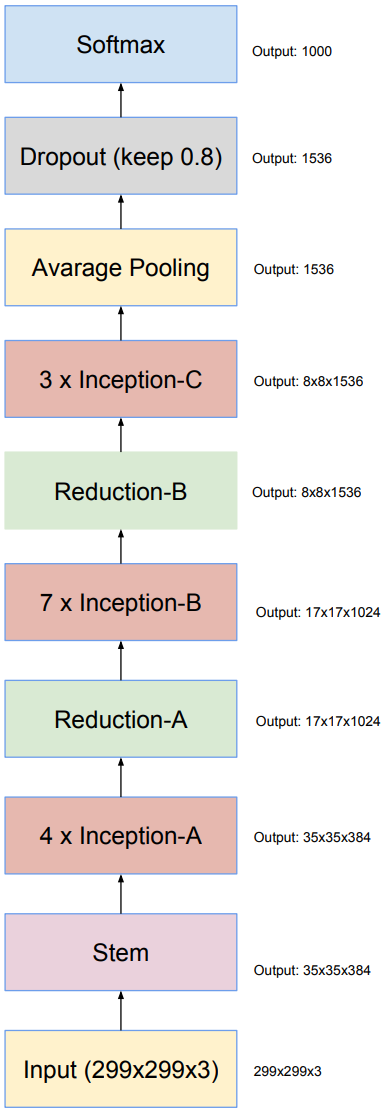
\includegraphics[angle=90,width=0.94\textwidth]{./Bilder/inceptionV4_architecture.png}
%\caption{InceptionV4 architecture \cite{InceptionV4}}
%\label{fig:inceptionv4}
%\end{figure}

\begin{figure}[!htb]
\centering
\begin{subfigure}[t]{0.47\textwidth}
   \resizebox{.99\linewidth}{!}{

\tikzset{every picture/.style={line width=0.75pt}} %set default line width to 0.75pt        

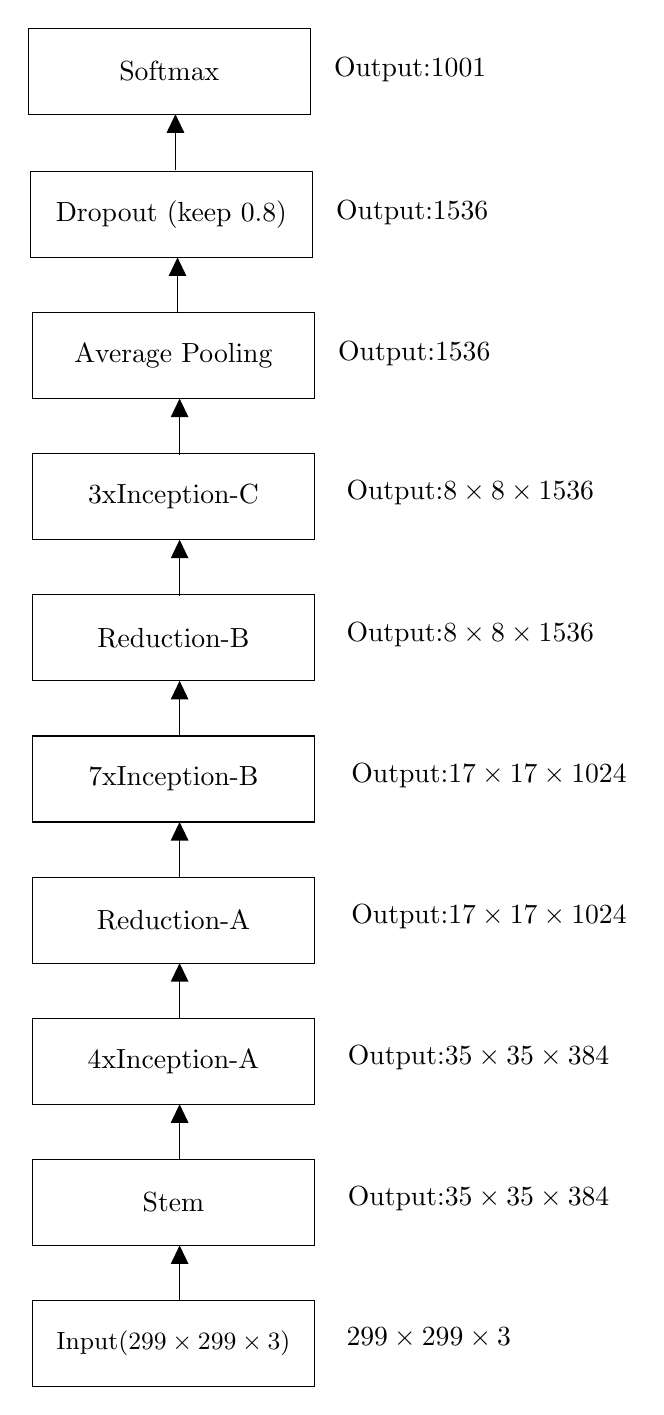
\begin{tikzpicture}[x=0.75pt,y=0.75pt,yscale=-1,xscale=1]
%uncomment if require: \path (0,742.7142868041992); %set diagram left start at 0, and has height of 742.7142868041992

%Flowchart: Process [id:dp9253173394290999] 
\draw   (98,621) -- (233.93,621) -- (233.93,662.43) -- (98,662.43) -- cycle ;
%Flowchart: Process [id:dp47578347996398307] 
\draw   (98,553) -- (233.93,553) -- (233.93,594.43) -- (98,594.43) -- cycle ;
%Straight Lines [id:da2925025767777827] 
\draw    (168.93,621.43) -- (168.93,596.43) ;
\draw [shift={(168.93,594.43)}, rotate = 450] [fill={rgb, 255:red, 0; green, 0; blue, 0 }  ][line width=0.75]  [draw opacity=0] (8.93,-4.29) -- (0,0) -- (8.93,4.29) -- cycle    ;

%Flowchart: Process [id:dp5382364848384393] 
\draw   (98,485) -- (233.93,485) -- (233.93,526.43) -- (98,526.43) -- cycle ;
%Straight Lines [id:da06940381159807729] 
\draw    (168.93,553.43) -- (168.93,528.43) ;
\draw [shift={(168.93,526.43)}, rotate = 450] [fill={rgb, 255:red, 0; green, 0; blue, 0 }  ][line width=0.75]  [draw opacity=0] (8.93,-4.29) -- (0,0) -- (8.93,4.29) -- cycle    ;

%Flowchart: Process [id:dp21301144435418706] 
\draw   (98,417) -- (233.93,417) -- (233.93,458.43) -- (98,458.43) -- cycle ;
%Straight Lines [id:da45627711718103714] 
\draw    (168.93,485.43) -- (168.93,460.43) ;
\draw [shift={(168.93,458.43)}, rotate = 450] [fill={rgb, 255:red, 0; green, 0; blue, 0 }  ][line width=0.75]  [draw opacity=0] (8.93,-4.29) -- (0,0) -- (8.93,4.29) -- cycle    ;

%Flowchart: Process [id:dp7231968775803179] 
\draw   (98,349) -- (233.93,349) -- (233.93,390.43) -- (98,390.43) -- cycle ;
%Straight Lines [id:da7165121439179447] 
\draw    (168.93,417.43) -- (168.93,392.43) ;
\draw [shift={(168.93,390.43)}, rotate = 450] [fill={rgb, 255:red, 0; green, 0; blue, 0 }  ][line width=0.75]  [draw opacity=0] (8.93,-4.29) -- (0,0) -- (8.93,4.29) -- cycle    ;

%Flowchart: Process [id:dp20620702942862734] 
\draw   (98,281) -- (233.93,281) -- (233.93,322.43) -- (98,322.43) -- cycle ;
%Straight Lines [id:da10564528480224444] 
\draw    (168.93,349.43) -- (168.93,324.43) ;
\draw [shift={(168.93,322.43)}, rotate = 450] [fill={rgb, 255:red, 0; green, 0; blue, 0 }  ][line width=0.75]  [draw opacity=0] (8.93,-4.29) -- (0,0) -- (8.93,4.29) -- cycle    ;

%Flowchart: Process [id:dp6409642010028676] 
\draw   (98,213) -- (233.93,213) -- (233.93,254.43) -- (98,254.43) -- cycle ;
%Straight Lines [id:da583110185704452] 
\draw    (168.93,281.43) -- (168.93,256.43) ;
\draw [shift={(168.93,254.43)}, rotate = 450] [fill={rgb, 255:red, 0; green, 0; blue, 0 }  ][line width=0.75]  [draw opacity=0] (8.93,-4.29) -- (0,0) -- (8.93,4.29) -- cycle    ;

%Flowchart: Process [id:dp747253235525678] 
\draw   (98,145) -- (233.93,145) -- (233.93,186.43) -- (98,186.43) -- cycle ;
%Straight Lines [id:da9482962038382927] 
\draw    (168.93,213.43) -- (168.93,188.43) ;
\draw [shift={(168.93,186.43)}, rotate = 450] [fill={rgb, 255:red, 0; green, 0; blue, 0 }  ][line width=0.75]  [draw opacity=0] (8.93,-4.29) -- (0,0) -- (8.93,4.29) -- cycle    ;

%Flowchart: Process [id:dp47103409298757426] 
\draw   (97,77) -- (232.93,77) -- (232.93,118.43) -- (97,118.43) -- cycle ;
%Straight Lines [id:da30249651940608824] 
\draw    (167.93,145.43) -- (167.93,120.43) ;
\draw [shift={(167.93,118.43)}, rotate = 450] [fill={rgb, 255:red, 0; green, 0; blue, 0 }  ][line width=0.75]  [draw opacity=0] (8.93,-4.29) -- (0,0) -- (8.93,4.29) -- cycle    ;

%Flowchart: Process [id:dp5661311837160838] 
\draw   (96,8) -- (231.93,8) -- (231.93,49.43) -- (96,49.43) -- cycle ;
%Straight Lines [id:da5142446239913938] 
\draw    (166.93,76.43) -- (166.93,51.43) ;
\draw [shift={(166.93,49.43)}, rotate = 450] [fill={rgb, 255:red, 0; green, 0; blue, 0 }  ][line width=0.75]  [draw opacity=0] (8.93,-4.29) -- (0,0) -- (8.93,4.29) -- cycle    ;


% Text Node
\draw (165.96,641.71) node  [align=left] {{\small Input($\displaystyle 299\times 299\times 3$)}};
% Text Node
\draw (165.96,573.71) node  [align=left] {Stem};
% Text Node
\draw (289,639) node  [align=left] {$\displaystyle 299\times 299\times 3$};
% Text Node
\draw (313,572) node  [align=left] {Output:$\displaystyle 35\times 35\times 384$};
% Text Node
\draw (165.96,505.71) node  [align=left] {4xInception-A};
% Text Node
\draw (313,504) node  [align=left] {Output:$\displaystyle 35\times 35\times 384$};
% Text Node
\draw (165.96,437.71) node  [align=left] {Reduction-A};
% Text Node
\draw (318,436) node  [align=left] {Output:$\displaystyle 17\times 17\times 1024$};
% Text Node
\draw (165.96,369.71) node  [align=left] {7xInception-B};
% Text Node
\draw (318,368) node  [align=left] {Output:$\displaystyle 17\times 17\times 1024$};
% Text Node
\draw (165.96,301.71) node  [align=left] {Reduction-B};
% Text Node
\draw (309,300) node  [align=left] {Output:$\displaystyle 8\times 8\times 1536$};
% Text Node
\draw (165.96,233.71) node  [align=left] {3xInception-C};
% Text Node
\draw (309,232) node  [align=left] {Output:$\displaystyle 8\times 8\times 1536$};
% Text Node
\draw (165.96,165.71) node  [align=left] {Average Pooling};
% Text Node
\draw (282,165) node  [align=left] {Output:$\displaystyle 1536$};
% Text Node
\draw (164.96,97.71) node  [align=left] {Dropout (keep $\displaystyle 0.8$)};
% Text Node
\draw (281,97) node  [align=left] {Output:$\displaystyle 1536$};
% Text Node
\draw (163.96,28.71) node  [align=left] {Softmax};
% Text Node
\draw (280,28) node  [align=left] {Output:$\displaystyle 1001$};


\end{tikzpicture}}
   \caption{InceptionV4 architecture \cite{InceptionV4}}
   \label{fig:inceptionv4Archi} 
\end{subfigure}%
\begin{subfigure}[t]{0.47\textwidth}
   %%Verify the architectures again
   \resizebox{.99\linewidth}{!}{

\tikzset{every picture/.style={line width=0.75pt}} %set default line width to 0.75pt        

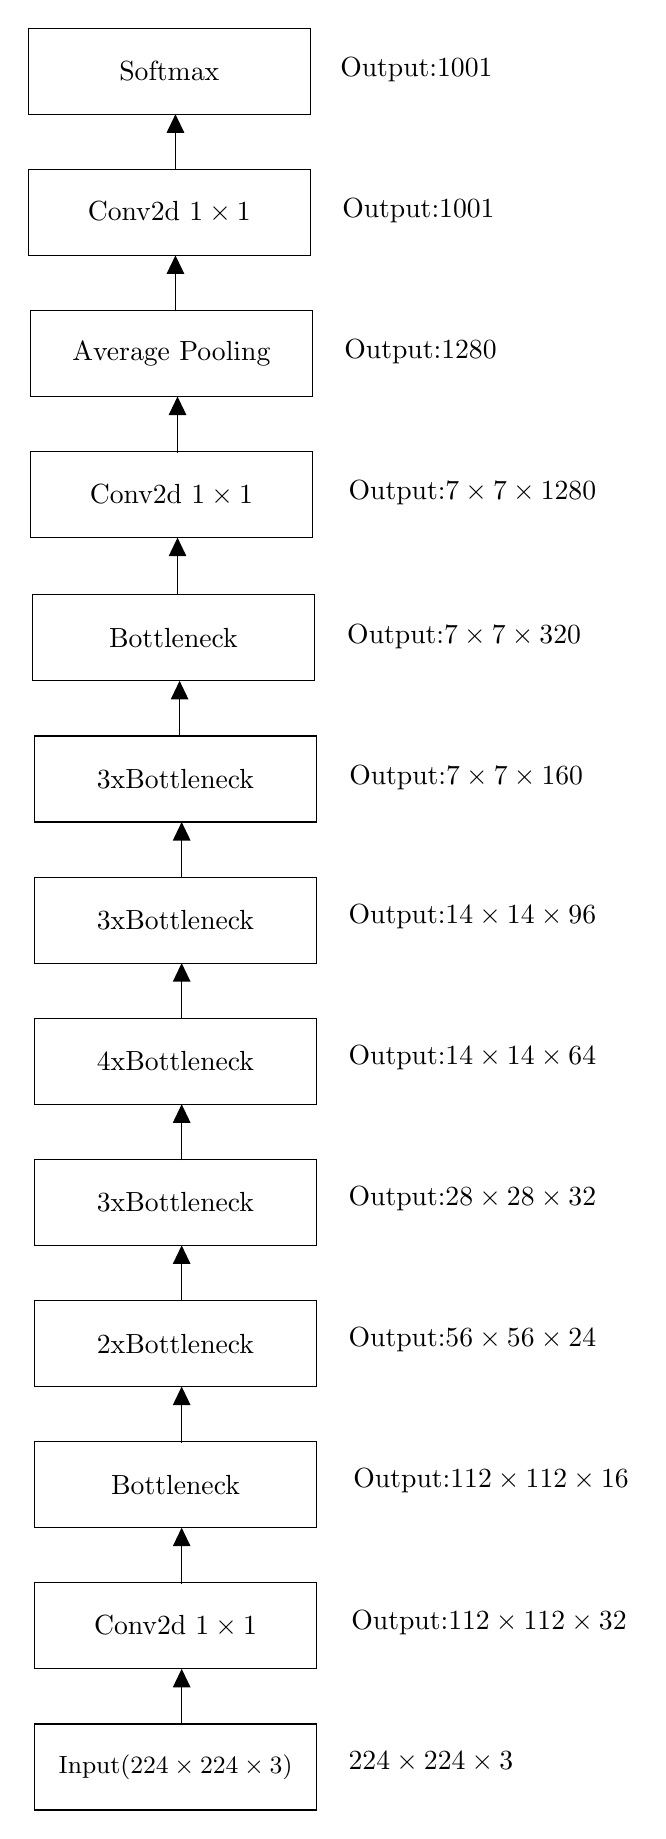
\begin{tikzpicture}[x=0.75pt,y=0.75pt,yscale=-1,xscale=1]
%uncomment if require: \path (0,948.6666870117188); %set diagram left start at 0, and has height of 948.6666870117188

%Flowchart: Process [id:dp9253173394290999] 
\draw   (98,897) -- (233.93,897) -- (233.93,938.43) -- (98,938.43) -- cycle ;
%Flowchart: Process [id:dp47578347996398307] 
\draw   (98,829) -- (233.93,829) -- (233.93,870.43) -- (98,870.43) -- cycle ;
%Straight Lines [id:da2925025767777827] 
\draw    (168.93,897.43) -- (168.93,872.43) ;
\draw [shift={(168.93,870.43)}, rotate = 450] [fill={rgb, 255:red, 0; green, 0; blue, 0 }  ][line width=0.75]  [draw opacity=0] (8.93,-4.29) -- (0,0) -- (8.93,4.29) -- cycle    ;

%Flowchart: Process [id:dp5382364848384393] 
\draw   (98,761) -- (233.93,761) -- (233.93,802.43) -- (98,802.43) -- cycle ;
%Straight Lines [id:da06940381159807729] 
\draw    (168.93,829.43) -- (168.93,804.43) ;
\draw [shift={(168.93,802.43)}, rotate = 450] [fill={rgb, 255:red, 0; green, 0; blue, 0 }  ][line width=0.75]  [draw opacity=0] (8.93,-4.29) -- (0,0) -- (8.93,4.29) -- cycle    ;

%Flowchart: Process [id:dp21301144435418706] 
\draw   (98,693) -- (233.93,693) -- (233.93,734.43) -- (98,734.43) -- cycle ;
%Straight Lines [id:da45627711718103714] 
\draw    (168.93,761.43) -- (168.93,736.43) ;
\draw [shift={(168.93,734.43)}, rotate = 450] [fill={rgb, 255:red, 0; green, 0; blue, 0 }  ][line width=0.75]  [draw opacity=0] (8.93,-4.29) -- (0,0) -- (8.93,4.29) -- cycle    ;

%Flowchart: Process [id:dp7231968775803179] 
\draw   (98,625) -- (233.93,625) -- (233.93,666.43) -- (98,666.43) -- cycle ;
%Straight Lines [id:da7165121439179447] 
\draw    (168.93,693.43) -- (168.93,668.43) ;
\draw [shift={(168.93,666.43)}, rotate = 450] [fill={rgb, 255:red, 0; green, 0; blue, 0 }  ][line width=0.75]  [draw opacity=0] (8.93,-4.29) -- (0,0) -- (8.93,4.29) -- cycle    ;

%Flowchart: Process [id:dp20620702942862734] 
\draw   (98,557) -- (233.93,557) -- (233.93,598.43) -- (98,598.43) -- cycle ;
%Straight Lines [id:da10564528480224444] 
\draw    (168.93,625.43) -- (168.93,600.43) ;
\draw [shift={(168.93,598.43)}, rotate = 450] [fill={rgb, 255:red, 0; green, 0; blue, 0 }  ][line width=0.75]  [draw opacity=0] (8.93,-4.29) -- (0,0) -- (8.93,4.29) -- cycle    ;

%Flowchart: Process [id:dp6409642010028676] 
\draw   (98,489) -- (233.93,489) -- (233.93,530.43) -- (98,530.43) -- cycle ;
%Straight Lines [id:da583110185704452] 
\draw    (168.93,557.43) -- (168.93,532.43) ;
\draw [shift={(168.93,530.43)}, rotate = 450] [fill={rgb, 255:red, 0; green, 0; blue, 0 }  ][line width=0.75]  [draw opacity=0] (8.93,-4.29) -- (0,0) -- (8.93,4.29) -- cycle    ;

%Flowchart: Process [id:dp747253235525678] 
\draw   (98,421) -- (233.93,421) -- (233.93,462.43) -- (98,462.43) -- cycle ;
%Straight Lines [id:da9482962038382927] 
\draw    (168.93,489.43) -- (168.93,464.43) ;
\draw [shift={(168.93,462.43)}, rotate = 450] [fill={rgb, 255:red, 0; green, 0; blue, 0 }  ][line width=0.75]  [draw opacity=0] (8.93,-4.29) -- (0,0) -- (8.93,4.29) -- cycle    ;

%Flowchart: Process [id:dp47103409298757426] 
\draw   (97,353) -- (232.93,353) -- (232.93,394.43) -- (97,394.43) -- cycle ;
%Straight Lines [id:da30249651940608824] 
\draw    (167.93,421.43) -- (167.93,396.43) ;
\draw [shift={(167.93,394.43)}, rotate = 450] [fill={rgb, 255:red, 0; green, 0; blue, 0 }  ][line width=0.75]  [draw opacity=0] (8.93,-4.29) -- (0,0) -- (8.93,4.29) -- cycle    ;

%Flowchart: Process [id:dp5661311837160838] 
\draw   (96,284) -- (231.93,284) -- (231.93,325.43) -- (96,325.43) -- cycle ;
%Straight Lines [id:da5142446239913938] 
\draw    (166.93,352.43) -- (166.93,327.43) ;
\draw [shift={(166.93,325.43)}, rotate = 450] [fill={rgb, 255:red, 0; green, 0; blue, 0 }  ][line width=0.75]  [draw opacity=0] (8.93,-4.29) -- (0,0) -- (8.93,4.29) -- cycle    ;

%Flowchart: Process [id:dp8648151912409288] 
\draw   (96,216) -- (231.93,216) -- (231.93,257.43) -- (96,257.43) -- cycle ;
%Straight Lines [id:da21788225541174455] 
\draw    (166.93,284.43) -- (166.93,259.43) ;
\draw [shift={(166.93,257.43)}, rotate = 450] [fill={rgb, 255:red, 0; green, 0; blue, 0 }  ][line width=0.75]  [draw opacity=0] (8.93,-4.29) -- (0,0) -- (8.93,4.29) -- cycle    ;

%Flowchart: Process [id:dp5915277931570215] 
\draw   (95,148) -- (230.93,148) -- (230.93,189.43) -- (95,189.43) -- cycle ;
%Straight Lines [id:da2169186042376452] 
\draw    (165.93,216.43) -- (165.93,191.43) ;
\draw [shift={(165.93,189.43)}, rotate = 450] [fill={rgb, 255:red, 0; green, 0; blue, 0 }  ][line width=0.75]  [draw opacity=0] (8.93,-4.29) -- (0,0) -- (8.93,4.29) -- cycle    ;

%Flowchart: Process [id:dp09241683513730559] 
\draw   (95,80) -- (230.93,80) -- (230.93,121.43) -- (95,121.43) -- cycle ;
%Straight Lines [id:da3985231842573671] 
\draw    (165.93,148.43) -- (165.93,123.43) ;
\draw [shift={(165.93,121.43)}, rotate = 450] [fill={rgb, 255:red, 0; green, 0; blue, 0 }  ][line width=0.75]  [draw opacity=0] (8.93,-4.29) -- (0,0) -- (8.93,4.29) -- cycle    ;


% Text Node
\draw (165.96,917.71) node  [align=left] {{\small Input($\displaystyle 224\times 224\times 3$)}};
% Text Node
\draw (165.96,849.71) node  [align=left] {Conv2d $\displaystyle 1\times 1$};
% Text Node
\draw (289,915) node  [align=left] {$\displaystyle 224\times 224\times 3$};
% Text Node
\draw (317,848) node  [align=left] {Output:$\displaystyle 112\times 112\times 32$};
% Text Node
\draw (165.96,781.71) node  [align=left] {Bottleneck};
% Text Node
\draw (318,780) node  [align=left] {Output:$\displaystyle 112\times 112\times 16$};
% Text Node
\draw (165.96,713.71) node  [align=left] {2xBottleneck};
% Text Node
\draw (309,712) node  [align=left] {Output:$\displaystyle 56\times 56\times 24$};
% Text Node
\draw (165.96,645.71) node  [align=left] {3xBottleneck};
% Text Node
\draw (309,644) node  [align=left] {Output:$\displaystyle 28\times 28\times 32$};
% Text Node
\draw (165.96,577.71) node  [align=left] {4xBottleneck};
% Text Node
\draw (309,576) node  [align=left] {Output:$\displaystyle 14\times 14\times 64$};
% Text Node
\draw (165.96,509.71) node  [align=left] {3xBottleneck};
% Text Node
\draw (309,508) node  [align=left] {Output:$\displaystyle 14\times 14\times 96$};
% Text Node
\draw (165.96,441.71) node  [align=left] {3xBottleneck};
% Text Node
\draw (306,441) node  [align=left] {Output:$\displaystyle 7\times 7\times 160$};
% Text Node
\draw (164.96,373.71) node  [align=left] {Bottleneck};
% Text Node
\draw (305,373) node  [align=left] {Output:$\displaystyle 7\times 7\times 320$};
% Text Node
\draw (163.96,304.71) node  [align=left] {Conv2d $\displaystyle 1\times 1$};
% Text Node
\draw (309,304) node  [align=left] {Output:$\displaystyle 7\times 7\times 1280$};
% Text Node
\draw (163.96,236.71) node  [align=left] {Average Pooling};
% Text Node
\draw (284,236) node  [align=left] {Output:$\displaystyle 1280$};
% Text Node
\draw (162.96,168.71) node  [align=left] {Conv2d $\displaystyle 1\times 1$};
% Text Node
\draw (283,168) node  [align=left] {Output:$\displaystyle 1001$};
% Text Node
\draw (162.96,100.71) node  [align=left] {Softmax};
% Text Node
\draw (282,100) node  [align=left] {Output:$\displaystyle 1001$};


\end{tikzpicture}}
   \caption{MobileNetV2 architecture \cite{DBLP:journals/corr/abs-1801-04381}}
   \label{fig:MobileNetArchi}
\end{subfigure}

\caption{Architectures of InceptionV4 and MobileNetV2}
%%NO DROPOUT AT INFERENCE
\end{figure}

\subsubsection{Input data}
We evaluate the performance of $2$, $4$, $8$ and $16$  megapixels (MP) \emph{PNG} images, as state of the art edge devices are capable of taking pictures with such high amounts of megapixels. This way the effect of different image sizes on the performance of the preprocessing step can be assessed. We also evaluate an image where no resizing is needed ($224\times224$ and $299\times299$ depending on the model) to study the impact of image resizing. A picture of a cat (see figure \ref{fig:cat}) scaled to the different sizes will serve as the picture for the experiments.
The sizes of the images in kilobytes as well as the according resolutions can be seen in table \ref{table:imagesOverview}. In the following, when we speak of $224^2/299^2$ or $0.05$MP images, we mean both $224\times224$ and $299\times299$ images.

\begin{table}[!htb]
\centering
%CITE inception params ned vergessen
%http://dgschwend.github.io/netscope/#/preset/inceptionv4
\caption{Overview of used image sizes}
\label{table:imagesOverview}
\begin{tabular}{@{}lll@{}}
\toprule
Image   & Resolution       & \emph{PNG} Size  \\ \midrule
$224^2$ & $224\times224$   & $83$KB    \\
$299^2$ & $299\times299$   & $141$KB   \\
$2$MP   & $1732\times1155$ & $2411$KB  \\
$4$MP   & $2449\times1633$ & $4309$KB  \\
$8$MP   & $3464\times2309$ & $7515$KB  \\
$16$MP  & $4899\times3266$ & $10077$KB \\ \bottomrule
\end{tabular}
\end{table}
\begin{figure}[!htb]
\centering
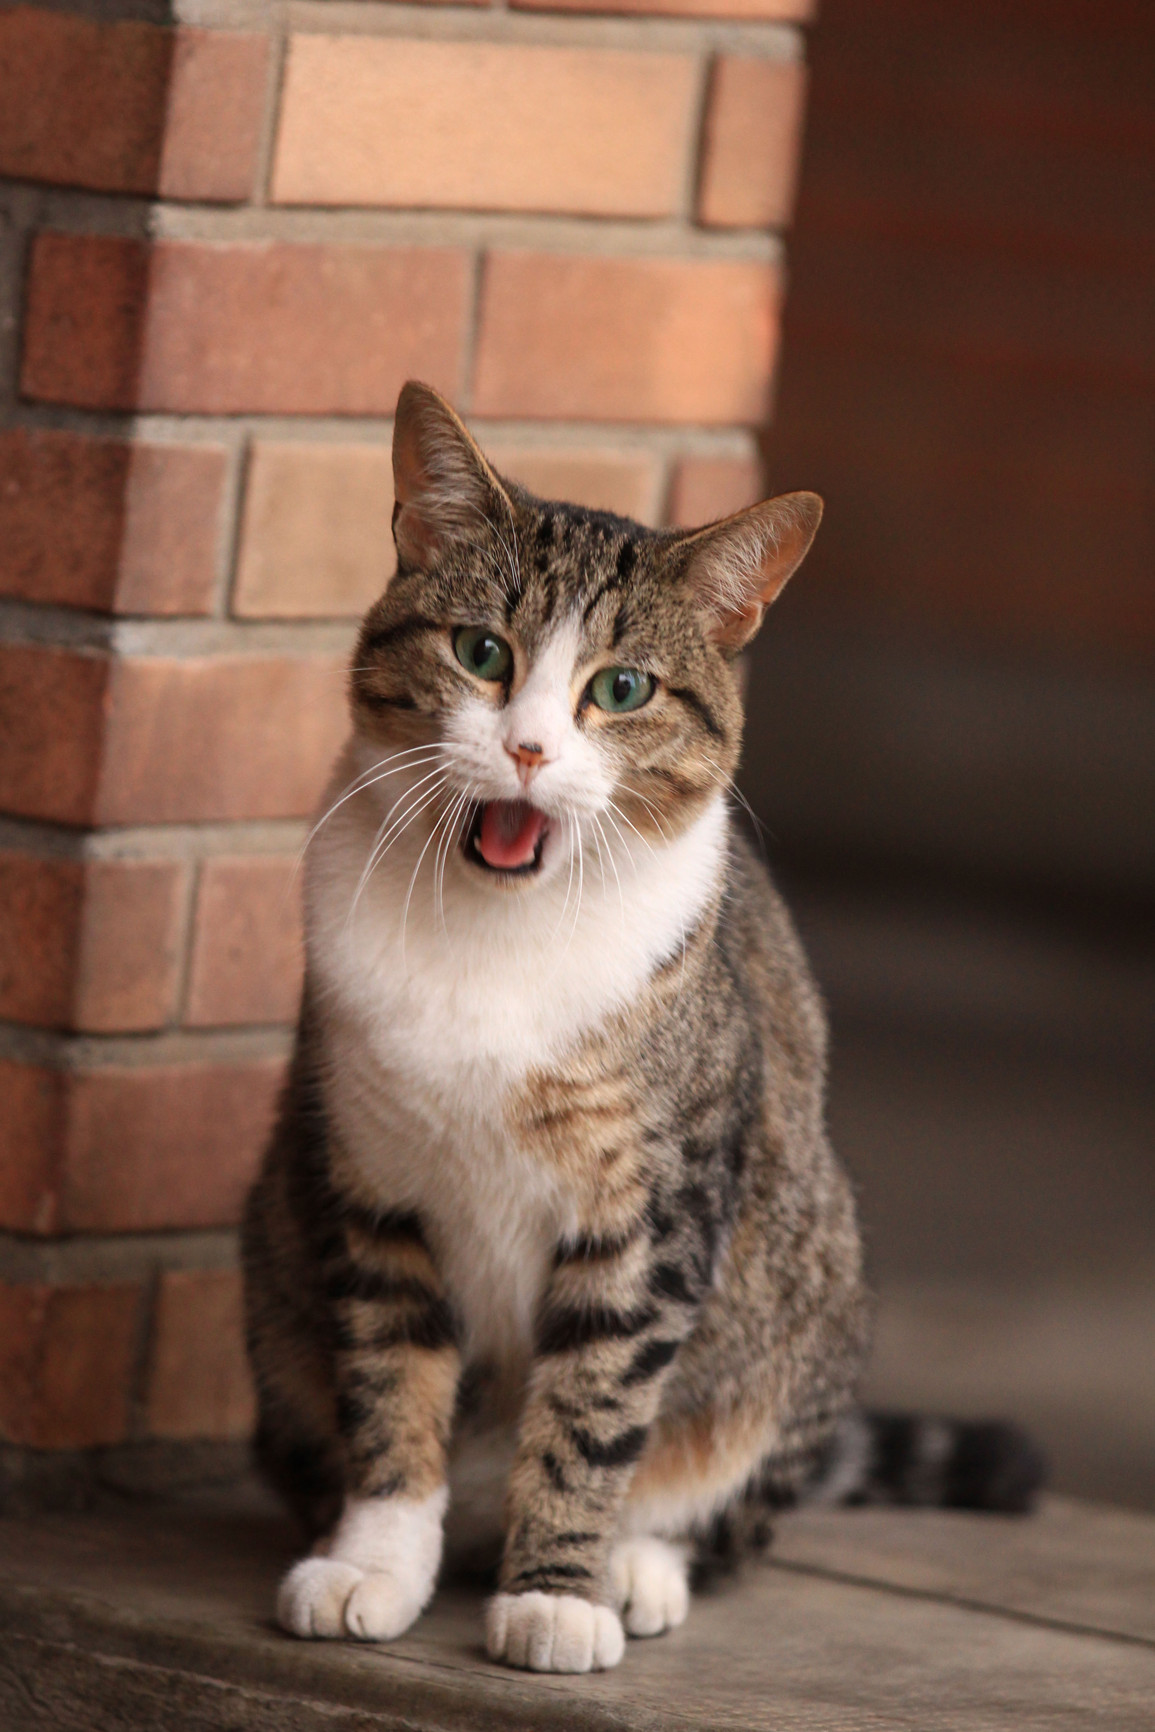
\includegraphics[width=0.3\textwidth]{./Bilder/European_cat_compressed.jpg}
\caption{Picture used for the experiments \cite{cat}}
\label{fig:cat}
\end{figure}
\paragraph{Batch Size}
%%mathe defs of throughput?
Another way to increase workload, except different images sizes, is to increase the batch size of a request.
Batch size denotes the number of images fed into the deep learning model in a single inference operation. 
Feeding more than one image to the network can lead to higher throughput, if enough computational power is available. This increase in throughput often comes at the cost of increased latency and general resource consumption.

To study these trade-offs, we conduct experiments with the following batch sizes: 1, 2, 16, 32. Since at the point of these benchmarks a batch size greater than one is not supported for the TensorFlow Lite versions of MobileNetV2 (both float and quantized), measurements with these batch sizes cannot be performed for the case of edge inference at this point.

\subsection{Factors}
Over the course of the benchmark execution, we study the effect of multiple factors on performance with different levels.
%%%293,performance analysis buch

\paragraph{Preprocessing Mode}
For the case of cloud inference, the major parts of the needed preprocessing are either done on the edge before sending the image to the cloud or done on the cloud. Therefore we evaluate both options.
\paragraph{Inference Mode}
The inference can either be performed on the edge or an a cloud-backend.
We expect significant trade-offs between these two inference options, especially for large deep learning models.


\paragraph{NNAPI}
The Android Neural Network API (NNAPI), presented in section \ref{chap:NNAPI}, is supposed to enhance the inference performance of TensorFlow Lite. Therefore we take a look into the effect of this framework.
%%Mention GPU use here
\paragraph{GPU Usage}
Since January 16 an experimental release of TensorFlow Lite supporting GPU usage on Android using OpenGL ES 3.1 Compute Shaders \cite{tfLiteGPU}.
So far only four public models and their operators are supported, including MobileNetV2, but not InceptionV4. 
Therefore we omit the test of this new feature in our experimentation, but our initial testing indicated that the use of NNAPI provides faster inference latencies for MobileNetV2 than the GPU version.
%%https://medium.com/tensorflow/tensorflow-lite-now-faster-with-mobile-gpus-developer-preview-e15797e6dee7
%experimental
%only mobilenet supported
%worse performance than NNAPI so far


\begin{figure}[!htb]
\centering
 \scalebox{.7}{%\documentclass[border=10pt]{standalone}
%\usepackage{tikz}
%\begin{document}
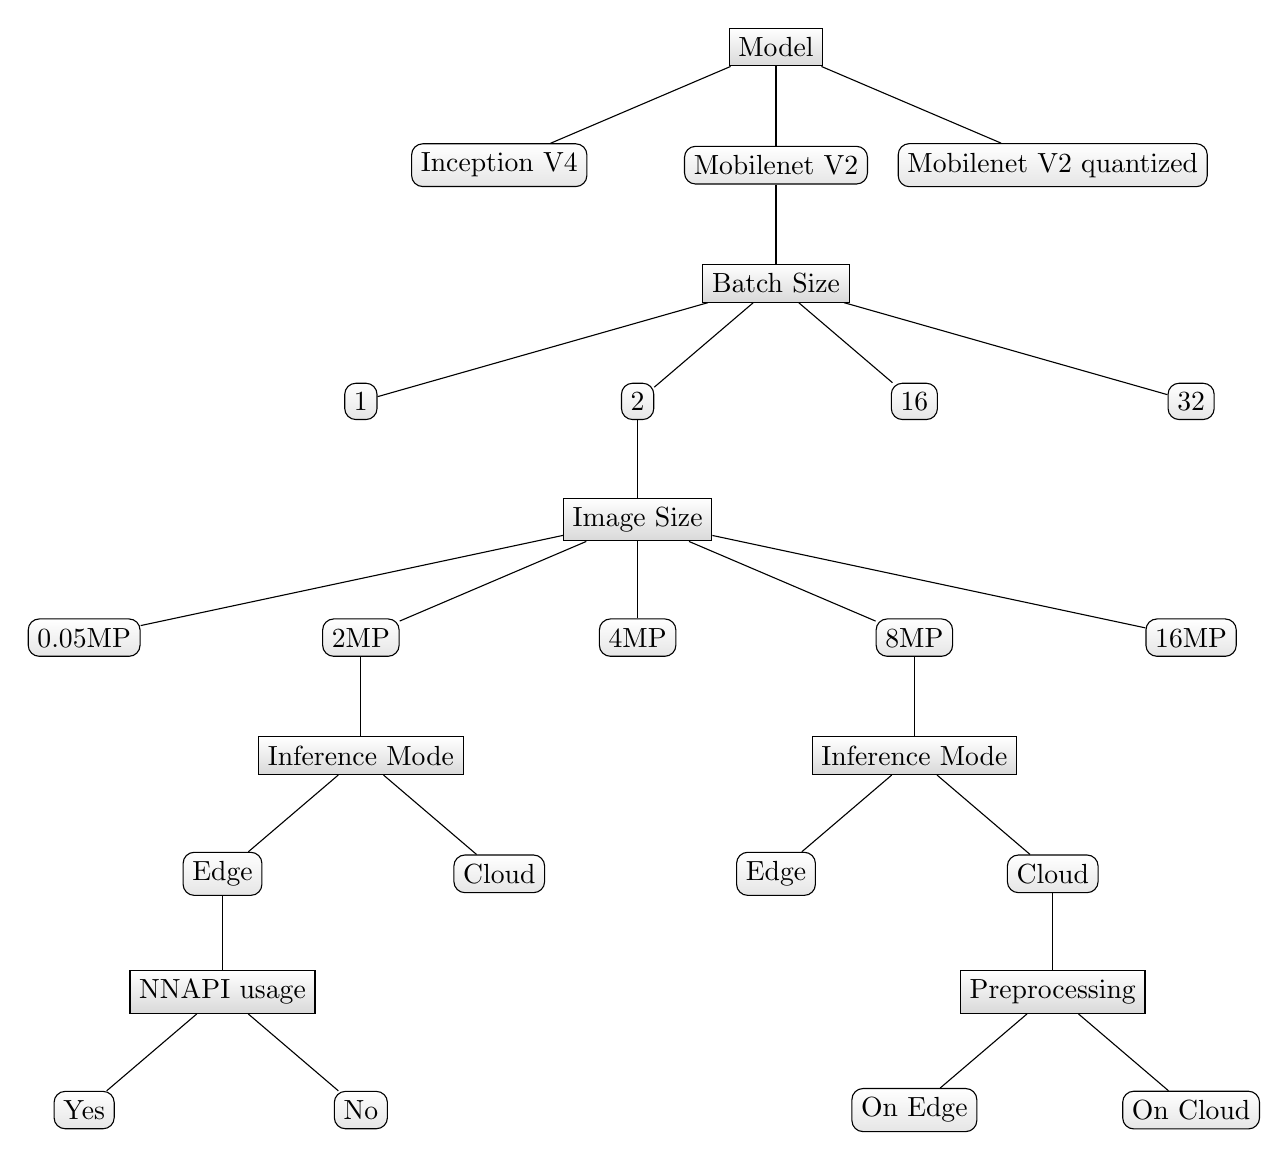
\begin{tikzpicture}[sibling distance=10em,
  param/.style={shape=rectangle,
    draw, align=center,
    top color=white, bottom color=gray!30},
  conf/.style={shape=rectangle, rounded corners,
    draw, align=center,
    top color=white, bottom color=gray!20}  ]  ]
    
  \node[param] {Model}
    child { node [conf]{Inception V4} }
    child { node [conf]{Mobilenet V2}
      child { node [param]{Batch Size}
        child { node [conf]{1} }
        child { node [conf]{2} 
            child { node [param]{Image Size}
                child { node [conf]{0.05MP}}
                child { node [conf]{2MP}
                child { node [param]{Inference Mode}
                        child { node[conf] {Edge}
                            child { node[param] {NNAPI usage}
                                 child { node[conf] {Yes}}
                                 child { node [conf]{No}}}}
                        child { node [conf]{Cloud}
                            }}}
                child { node [conf]{4MP}
                    }
                child { node [conf]{8MP}
                child { node [param]{Inference Mode}
                        child { node[conf] {Edge}}
                        child { node [conf]{Cloud}
                            child { node [param]{Preprocessing}
                               child { node [conf]{On Edge}}
                                child { node [conf]{On Cloud}}}}}}
                child { node [conf]{16MP}}}}
        child { node[conf] {16} }
        child { node [conf]{32} }} }
    child { node [conf]{Mobilenet V2 quantized} };
\end{tikzpicture}
%\end{document}}

\caption{Excerpt of the executed parameter configurations}
\label{fig:tree}
\end{figure}


\vspace{15pt}
Figure \ref{fig:tree} shows a part of our parameter tree, including both workload and factors. In theory, there would be $240$ different parameter configurations, but due to a number of reasons, the number of different configurations reduced to 113 in total.
First, the usage of NNAPI is independent of the image size hence we only perform experiments without NNAPI for one image size. Also the usage of NNAPI leads to a way better performance for edge inference and we want to compare edge and cloud inference, so we only carry out experiments without NNAPI for a batch size of one.
We omit the cloud inference for the quantized MobileNetV2 because the model is so small the network overhead would be overwhelming.
Lastly, due to lack of support certain operations in TensorFlow Lite for the MobileNetV2 models, we can not perform inference experiment for MobileNetV2 with a batch size larger than one.

\section{Android Benchmark Framework}
\label{chap:androidApp}
To conduct the benchmarks for both edge and cloud inference we developed and implemented an Android benchmark framework using Kotlin.
This system implements all functionality needed to simulate the defined workloads and parameters and perform the inference on either the Android device itself or send the image to a cloud-backend.
For both preprocessing and inference the application logs metrics such as inference latency and time of the experiments and stores them to a \emph{CSV} file, which then can be used to evaluation purposes.

Both edge and cloud inference implementations are based on the example implementations in the respective GitHub repositories\footnote{https://github.com/tensorflow/tensorflow/tree/master/tensorflow/lite/java/demo}\footnote{https://github.com/tensorflow/serving/blob/master/tensorflow\_serving/example/resnet\_client\_grpc.py} to ensure optimal performance. 


\begin{figure}[!htb]
\centering
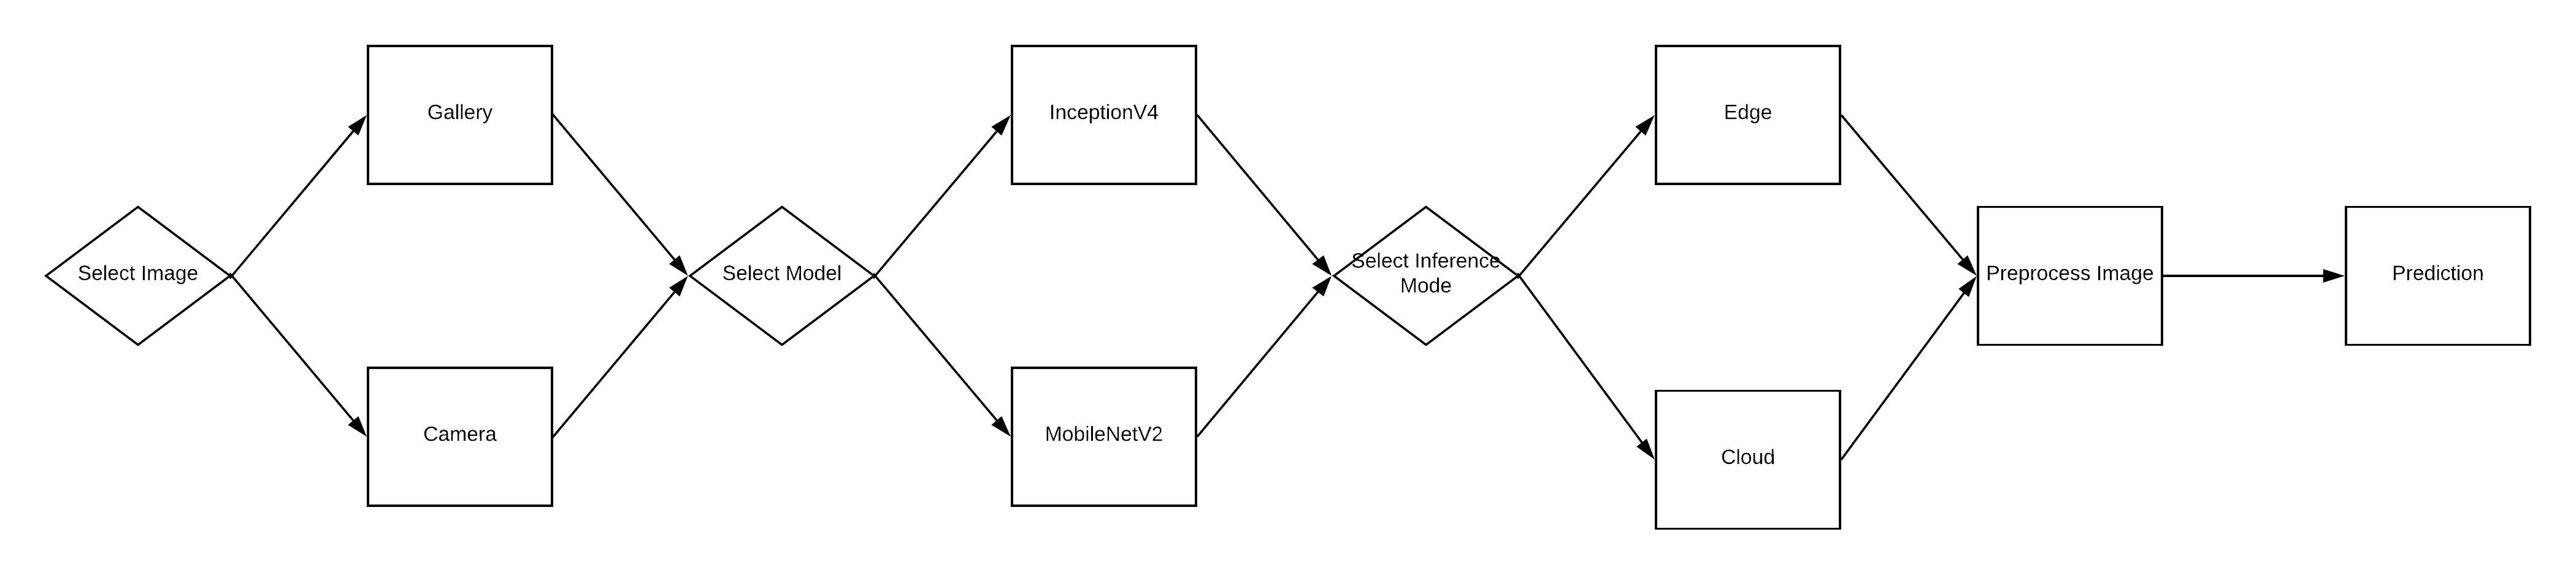
\includegraphics[width=0.99\textwidth]{./Bilder/FlowChart_App.png}
\caption{Flowchart of the Benchmark Application showing the whole inference process of selecting an image until getting a prediction}
\label{fig:app}
\end{figure}
In figure \ref{fig:app} the work-flow to perform the inference is seen. First, an image needs to be selected. Afterwards, the image classification model needs to be chosen. Now the user selects whether the inference should be performed on the cloud-backend or directly on the edge device, in this case, an Android phone. In the case of edge inference, it needs to be decided if the NNAPI should be used by TensorFlow Lite. For cloud inference, the preprocessing mode needs to be selected (edge/cloud). Now the preprocessing operations can be performed based on the previously selected options (Even for the case of cloud inference with cloud preprocessing some preprocessing needs to be done at the edge beforehand like building a \emph{PredictRequest} containing the request for the cloud-backend). Now, that the input is preprocessed, the actual inference is performed as the last step, resulting in a prediction. For both preprocessing and inference the measurements mentioned in section \ref{chap:insta_measurements} are logged.

\begin{figure}[htb]
\centering
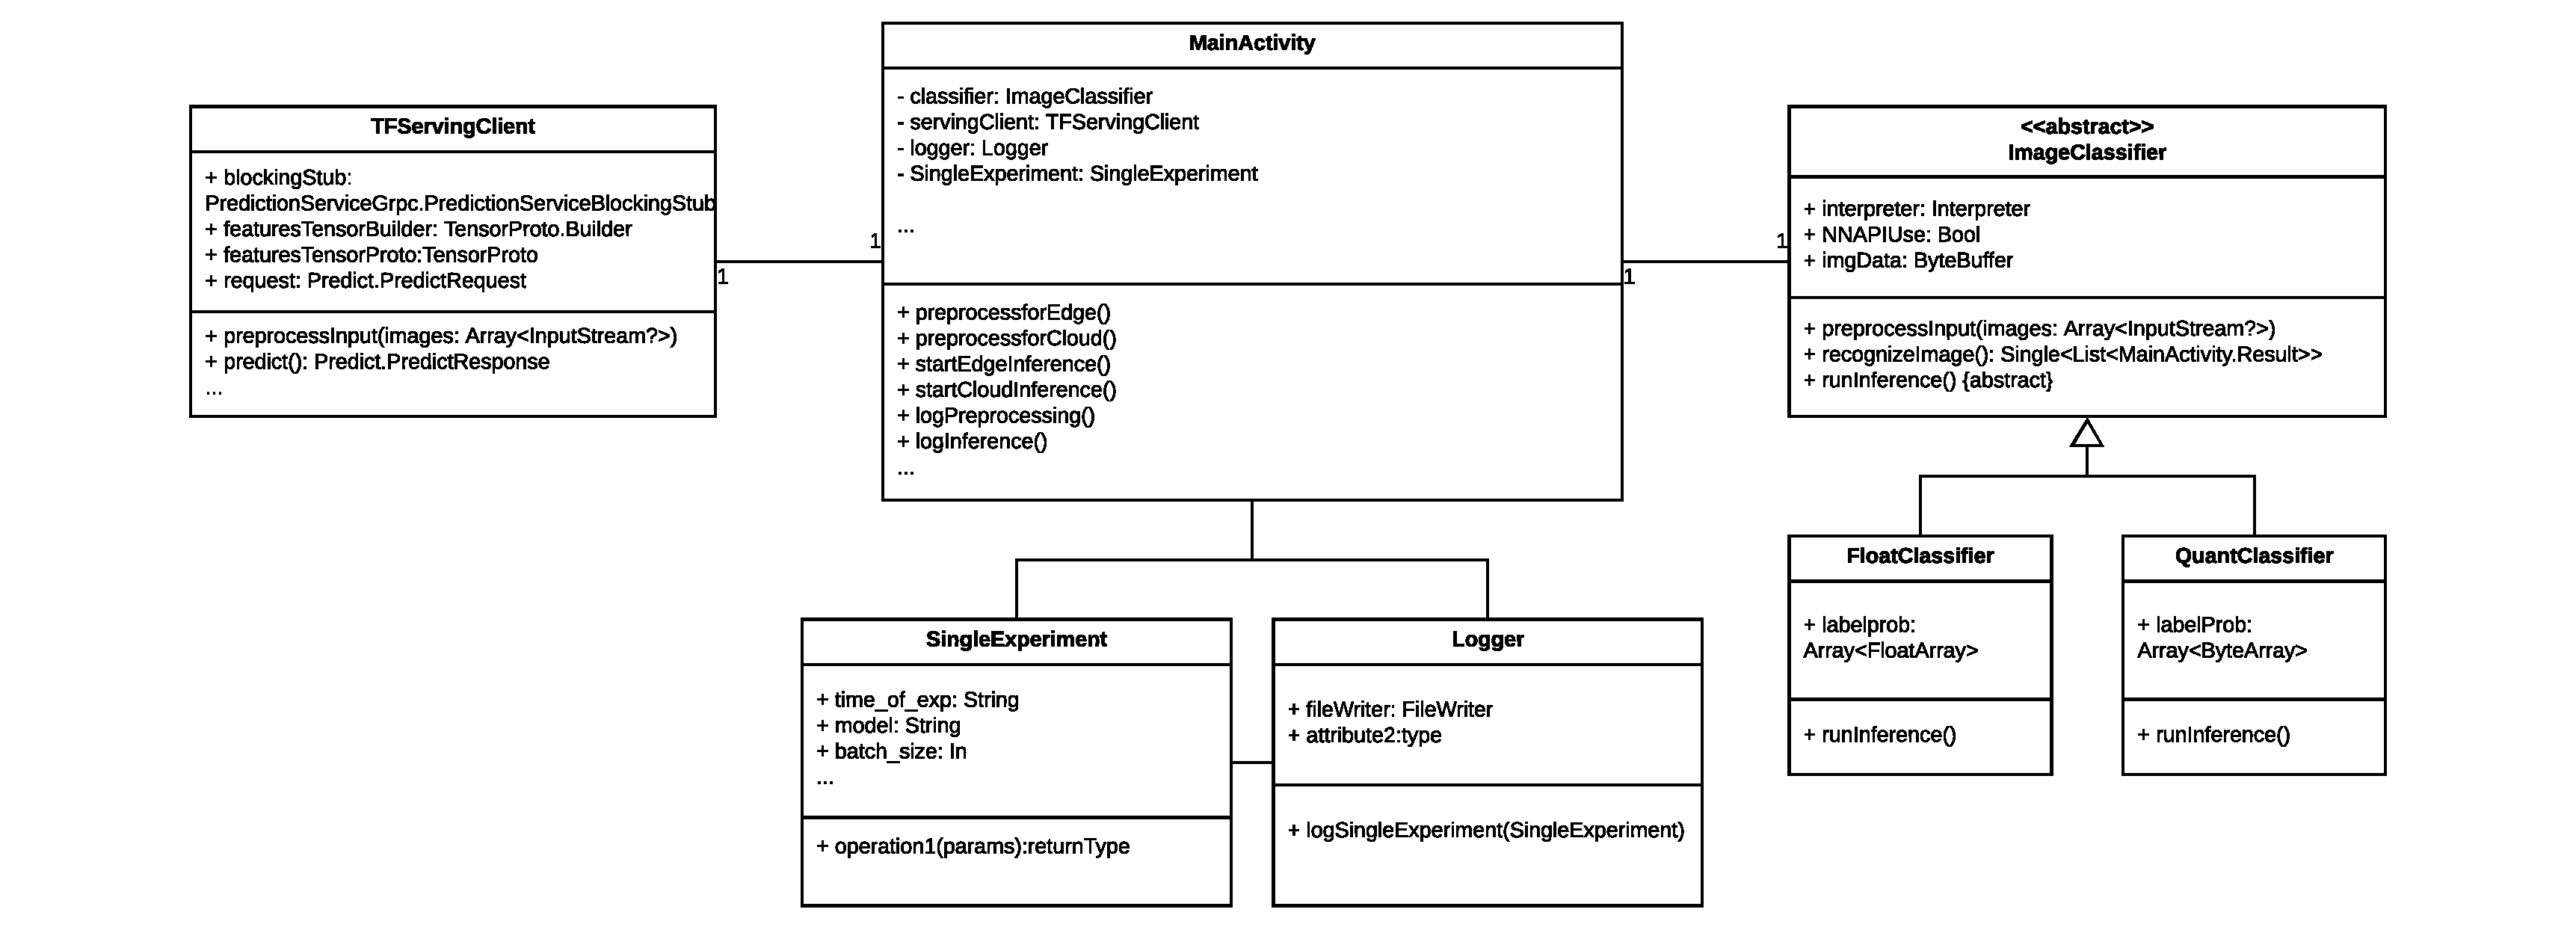
\includegraphics[width=0.99\textwidth]{./Bilder/UML.pdf}
\caption{UML class diagram of the benchmark application}
\label{fig:UML}
\end{figure}
Figure \ref{fig:UML} depicts a UML class diagram of the application featuring the most important classes, functions and variables. 
The main class is called \emph{MainActivity} and implements all of the graphical aspects. 
The \emph{MainActivity} handles requests for both cloud and edge inference by delegating the requests to instances of the classes \emph{TFServingClient} and \emph{ImageClassifier}, respectively. Both of these classes also take care of the preprocessing steps.
The abstract class \emph{ImageClassifier} has two subclasses \emph{FloatClassifier} and \emph{QuantClassifier}. The first class runs the inference for floating point models and the second for quantized models.
This separation is needed since these different model types require different input and output types.

The \emph{MainActivity} writes the collected measurements and the parameter configurations of an experiment to an instance of \emph{SingleExperiment}. After the experiment is completed \emph{MainActivity} tells a \emph{Logger} instance to save the contents of the \emph{SingleExperiment} object. The Logger then saves all collected data to a \emph{CSV} file.

\subsection{Preprocessing}
%%mention png
For the case of image classification, the images need to have the correct size ($224\times224$ for MobileNetV2 and $299\times299$ for InceptionV4) and the \emph{RGB} values need to be normalized to the interval $[-1,1]$. After preprocessing the image has been transformed into the shape $224\times224\times3$ with all values between $[-1,1]$, where the first two dimensions represent the image height and width, while the last dimension represents the number of channels (3 since the images are \emph{RGB}).
\begin{figure}[!htb]
\centering


\tikzset{every picture/.style={line width=0.75pt}} %set default line width to 0.75pt        

\begin{tikzpicture}[x=0.75pt,y=0.75pt,yscale=-1,xscale=1]
%uncomment if require: \path (0,484.3333282470703); %set diagram left start at 0, and has height of 484.3333282470703

%Shape: Square [id:dp1081653036325061] 
\draw  [fill={rgb, 255:red, 0; green, 0; blue, 255 }  ,fill opacity=1 ] (217.67,92) -- (317,92) -- (317,191.33) -- (217.67,191.33) -- cycle ;
%Shape: Square [id:dp8785233930816818] 
\draw  [fill={rgb, 255:red, 0; green, 255; blue, 0 }  ,fill opacity=1 ] (207.67,100) -- (307,100) -- (307,199.33) -- (207.67,199.33) -- cycle ;
%Image [id:dp7451570314710638] 
\draw (67,158.49) node  {\includegraphics[width=52.5pt,height=78.73pt]{Bilder/European_cat_02_16_mp.jpg}};
%Shape: Square [id:dp7219434207477922] 
\draw  [fill={rgb, 255:red, 255; green, 0; blue, 0 }  ,fill opacity=1 ] (199.67,110) -- (299,110) -- (299,209.33) -- (199.67,209.33) -- cycle ;
%Straight Lines [id:da9021822569380376] 
\draw    (106.17,157.33) -- (177.17,157.33) ;
\draw [shift={(179.17,157.33)}, rotate = 180] [fill={rgb, 255:red, 0; green, 0; blue, 0 }  ][line width=0.75]  [draw opacity=0] (8.93,-4.29) -- (0,0) -- (8.93,4.29) -- cycle    ;

%Straight Lines [id:da9159956987115614] 
\draw    (337.17,157.33) -- (408.17,157.33) ;
\draw [shift={(410.17,157.33)}, rotate = 180] [fill={rgb, 255:red, 0; green, 0; blue, 0 }  ][line width=0.75]  [draw opacity=0] (8.93,-4.29) -- (0,0) -- (8.93,4.29) -- cycle    ;

%Straight Lines [id:da07325949392344144] 
\draw  [dash pattern={on 0.84pt off 2.51pt}]  (232.17,121.33) -- (277.17,121.33) ;


%Straight Lines [id:da9028616351053764] 
\draw  [dash pattern={on 0.84pt off 2.51pt}]  (233.17,196.33) -- (278.17,196.33) ;


%Straight Lines [id:da27535102010063794] 
\draw  [dash pattern={on 0.84pt off 2.51pt}]  (217.17,136.33) -- (217.17,184.33) ;


%Straight Lines [id:da9334949593538635] 
\draw  [dash pattern={on 0.84pt off 2.51pt}]  (286.17,133.33) -- (286.17,181.33) ;


%Straight Lines [id:da021722670153532242] 
\draw  [dash pattern={on 0.84pt off 2.51pt}]  (228.17,131.33) -- (278.17,183.33) ;


%Shape: Square [id:dp4109817022076603] 
\draw  [fill={rgb, 255:red, 255; green, 255; blue, 255 }  ,fill opacity=1 ] (449.67,90) -- (549,90) -- (549,189.33) -- (449.67,189.33) -- cycle ;
%Shape: Square [id:dp544671777438523] 
\draw  [fill={rgb, 255:red, 255; green, 255; blue, 255 }  ,fill opacity=1 ] (439.67,98) -- (539,98) -- (539,197.33) -- (439.67,197.33) -- cycle ;
%Shape: Square [id:dp9050599364199439] 
\draw  [fill={rgb, 255:red, 255; green, 255; blue, 255 }  ,fill opacity=1 ] (431.67,108) -- (531,108) -- (531,207.33) -- (431.67,207.33) -- cycle ;
%Straight Lines [id:da02360170094364733] 
\draw  [dash pattern={on 0.84pt off 2.51pt}]  (455.17,120.33) -- (500.17,120.33) ;


%Straight Lines [id:da10167634289204797] 
\draw  [dash pattern={on 0.84pt off 2.51pt}]  (455.17,194.33) -- (500.17,194.33) ;


%Straight Lines [id:da23003293896688182] 
\draw  [dash pattern={on 0.84pt off 2.51pt}]  (443.17,135.33) -- (443.17,183.33) ;


%Straight Lines [id:da28496973593396335] 
\draw  [dash pattern={on 0.84pt off 2.51pt}]  (521.17,134.33) -- (521.17,182.33) ;


%Straight Lines [id:da06739883279353798] 
\draw  [dash pattern={on 0.84pt off 2.51pt}]  (452.17,127.33) -- (514.17,183.33) ;



% Text Node
\draw (250,217) node  [align=left] {$\displaystyle 224$};
% Text Node
\draw (188.17,157.33) node [rotate=-270] [align=left] {$\displaystyle 224$};
% Text Node
\draw (314,202) node [rotate=-319.82] [align=left] {$\displaystyle 3$};
% Text Node
\draw (141,170) node  [align=left] {Resizing};
% Text Node
\draw (371,171) node  [align=left] {Normalization};
% Text Node
\draw (215.67,197.33) node  [align=left] {$\displaystyle 255$};
% Text Node
\draw (216,120) node  [align=left] {$\displaystyle 255$};
% Text Node
\draw (287,196) node  [align=left] {$\displaystyle 0$};
% Text Node
\draw (286,120) node  [align=left] {$\displaystyle 0$};
% Text Node
\draw (442.67,194.33) node  [align=left] {$\displaystyle 1$};
% Text Node
\draw (444,118) node  [align=left] {$\displaystyle 1$};
% Text Node
\draw (519,193) node  [align=left] {$\displaystyle -1$};
% Text Node
\draw (518,118) node  [align=left] {$\displaystyle -1$};
% Text Node
\draw (421.17,155.33) node [rotate=-270] [align=left] {$\displaystyle 224$};
% Text Node
\draw (484,215) node  [align=left] {$\displaystyle 224$};
% Text Node
\draw (546,203) node [rotate=-319.82] [align=left] {$\displaystyle 3$};
% Text Node
\draw (67,220) node  [align=left] {$\displaystyle 1633$};
% Text Node
\draw (22,153) node [rotate=-270.5] [align=left] {$\displaystyle 2449$};
% Text Node
\draw (69,98) node  [align=left] {{\scriptsize source: [SeL] }};


\end{tikzpicture}
\caption{Preprocessing steps for image classification: Resizing to the model input size and normalization of the pixel values to $[-1,1]$}
\label{fig:prepro}
\end{figure}
\subsubsection{Edge Preprocessing}
\label{chap:preproImpl}
In the case of edge preprocessing all preprocessing steps are done on the edge device, meaning that the input can be fed directly into the neural network afterwards, either on the edge device itself or on a cloud-backend.
We perform these steps the following way: After loading the \emph{PNG} image into an \emph{InputStream} we create a scaled Bitmap of the image (scaled to either $224\times224$ or $299\times299$) by calling the \emph{createScaledBitmap} function. 
Afterwards, we normalize the \emph{RGB} values to $[-1,1]$ during the conversion from the bitmap to a \emph{ByteBuffer}. 
For the case of float models, this buffer contains all the pixels in float format and for the quantized model in bytes since quantized models work with lower representations.
%%%mehr erklären?
We do this conversion since feeding \emph{ByteBuffers} to TensorFlow Lite is performance enhancing. %add cite here
For cloud inference we then construct \emph{PredictRequest} object containing this \emph{ByteBuffer}.

For batch size larger than one we parallelize the preprocessing to speed up the preprocessing latency at the cost of higher maximum memory consumption. We start $n$ threads, where each thread is preprocessing one image in the way described above. After each image is preprocessed we concatenate all \emph{ByteBuffers} into a single one, which then can be fed to the TensorFlow Lite interpreter. Note that $n$ is determined by both batch size and available CPU cores on the edge device. There are never more threads than available cores, but if the batch size is smaller than the number of cores, we only start $n$ threads, where $n$ is the batch size. 

\subsubsection{Cloud Preprocessing}

In the case of cloud inference, the images can also be preprocessed directly at the cloud, resulting in nearly no preprocessing done at the edge. While the resizing and scaling steps are no longer done on the edge, the image still needs to be converted into a \emph{PredictRequest} object that TensorFlow Serving can handle.
To achieve this we load the \emph{PNG} image into an \emph{InputStream}, convert it to a \emph{ByteArray} which then can be feed to the \emph{PredictRequest} object as a \emph{ByteString}. 

%Add TensorFlow Serving preprocessing here


\subsection{Inference}
To get the predictions for our now preprocessed image, we need to run the inference operation of the inference framework with the deep learning model loaded, which is loaded either directly at the edge or the remote cloud-backend. 
The inference is done using the steps described in section \ref{chap:TFLite} (TensorFlow Lite) and \ref{chap:TFServing} (TensorFlow Serving).
\subsubsection{Edge Inference}
To perform the inference operation we need to pass two things to the \emph{run} function of an interpreter of TensorFlow Lite: The \emph{ByteBuffer} created in the preprocessing step and an array (float models: \emph{FloatArray}, quantized models: \emph{ByteArray}) with the length 1001 (number of classes). TensorFlow lite then writes the confidence levels of the different classes to this array. We then sort the array for the five classes with the highest confidence and print them to the screen.

\subsubsection{Cloud Inference}
\label{chap:CloudInfImpl}

For the cloud inference we send the \emph{PredictRequest} object created in the preprocessing process to the TensorFlow Serving server over a plaintext gRPC channel.
If the input has been preprocessed at the edge beforehand, Tensorflow Serving can perform the model inference directly.
If the input has not been preprocessed beforehand, the input arrives at the server in the \emph{PNG} format, therefore we first decode them with \emph{tf.image.decode\_jpeg}, then resize with \emph{tf.image.resize\_bilinear} and finally normalize the tensor values to $[-1,1]$ using the the \emph{subtract} and \emph{multiply} functions. Now the input has the same shape as if they would have been preprocessed at the edge can be fed to the actual model graphs.

\subsection{Instrumentation}
\label{chap:insta_measurements}
In the following section we describe how we measure the performance metrics defined in \ref{chap:metrics}.
We conduct the measurements either directly in the source code or by using Android Studio Profiler\footnote{https://developer.android.com/studio/profile/} (Version 3.3). Since Android Studio cannot collect all metrics the way we wanted, we wanted to use Trepn\footnote{https://developer.qualcomm.com/software/trepn-power-profiler} as a secondary profiling application. But since Trepn does not support our test device, we had to omit measurements of these metrics.

In the following definitions, $t_{start}$ denotes the starting point of either the preprocessing or inference, while $t_{end}$ denotes the end point of the respective process.
\subsubsection{Latency}
We measure $Latency_{preprocessing}$ by measuring the time difference between the start and end of the preprocessing process.
Note that all latency measurements are reported in milliseconds(ms).
\begin{equation*}
\begin{gathered}
Latency_{preprocessing} = t_{endPreprocessing} - t_{startPreprocessing}
\end{gathered}
\end{equation*}
To measure inference latency we need to distinguish between edge and cloud inference, since for the latter the network latency needs to be considered.

\paragraph{Edge Inference}To measure edge inference latency we measure the time the TensorFlow Lite interpreter needs to run the inference operation on the loaded model given the input image.
\begin{equation*}
\begin{gathered}
Latency_{inference} = t_{endInference} - t_{startInference}
\end{gathered}
\end{equation*}
\paragraph{Cloud Inference}
To measure the cloud inference latency we need to measure two latencies, which combined yield $Latency_{inference}$. The first latency is  $Latency_{server}$. This server latency describes the time difference between the point where TensorFlow Serving receives the inference request and the point in time where TensorFlow Serving sends the response back to the client.
The second latency $Latency_{network}$ denotes the time the prediction request needs to reach the cloud-backend and the time the response need from the server back to the TensorFlow Serving client..
These latencies are illustrated in figure \ref{fig:serverLat}.
\begin{figure}[!htb]
\centering


\tikzset{every picture/.style={line width=0.75pt}} %set default line width to 0.75pt        

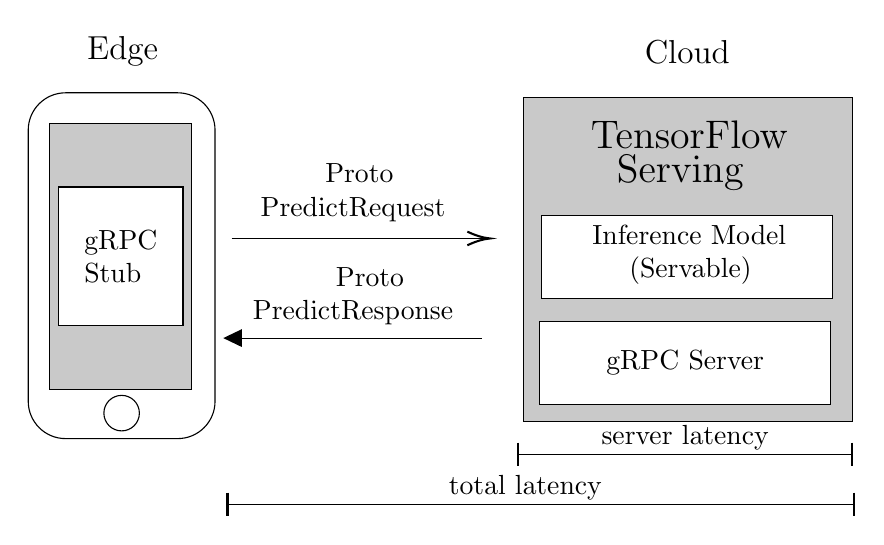
\begin{tikzpicture}[x=0.75pt,y=0.75pt,yscale=-1,xscale=1]
%uncomment if require: \path (0,300); %set diagram left start at 0, and has height of 300

%Straight Lines [id:da7072764839644827] 
\draw    (149.5,277) -- (451.5,277) ;
\draw [shift={(451.5,277)}, rotate = 180] [color={rgb, 255:red, 0; green, 0; blue, 0 }  ][line width=0.75]    (0,5.59) -- (0,-5.59)   ;
\draw [shift={(149.5,277)}, rotate = 180] [color={rgb, 255:red, 0; green, 0; blue, 0 }  ][line width=0.75]    (0,5.59) -- (0,-5.59)   ;
%Straight Lines [id:da9536138531960994] 
\draw    (289.5,253) -- (450.5,253) ;
\draw [shift={(450.5,253)}, rotate = 180] [color={rgb, 255:red, 0; green, 0; blue, 0 }  ][line width=0.75]    (0,5.59) -- (0,-5.59)   ;
\draw [shift={(289.5,253)}, rotate = 180] [color={rgb, 255:red, 0; green, 0; blue, 0 }  ][line width=0.75]    (0,5.59) -- (0,-5.59)   ;
%Shape: Rectangle [id:dp8902536871651789] 
\draw  [fill={rgb, 255:red, 201; green, 201; blue, 201 }  ,fill opacity=1 ] (63.91,93.69) -- (132.34,93.69) -- (132.34,221.63) -- (63.91,221.63) -- cycle ;
%Rounded Rect [id:dp41557214204551274] 
\draw   (53.5,96.82) .. controls (53.5,86.88) and (61.56,78.82) .. (71.5,78.82) -- (125.5,78.82) .. controls (135.44,78.82) and (143.5,86.88) .. (143.5,96.82) -- (143.5,227.43) .. controls (143.5,237.37) and (135.44,245.43) .. (125.5,245.43) -- (71.5,245.43) .. controls (61.56,245.43) and (53.5,237.37) .. (53.5,227.43) -- cycle ;
%Shape: Ellipse [id:dp8878397246816687] 
\draw   (89.95,233.16) .. controls (89.95,228.43) and (93.78,224.6) .. (98.5,224.6) .. controls (103.22,224.6) and (107.05,228.43) .. (107.05,233.16) .. controls (107.05,237.88) and (103.22,241.71) .. (98.5,241.71) .. controls (93.78,241.71) and (89.95,237.88) .. (89.95,233.16) -- cycle ;
%Straight Lines [id:da5813802620369573] 
\draw    (151.48,149) -- (274,149) ;
\draw [shift={(276,149)}, rotate = 540] [color={rgb, 255:red, 0; green, 0; blue, 0 }  ][line width=0.75]    (10.93,-3.29) .. controls (6.95,-1.4) and (3.31,-0.3) .. (0,0) .. controls (3.31,0.3) and (6.95,1.4) .. (10.93,3.29)   ;

%Straight Lines [id:da16220168680973557] 
\draw    (149.48,197) -- (272,197) ;

\draw [shift={(147.48,197)}, rotate = 360] [fill={rgb, 255:red, 0; green, 0; blue, 0 }  ][line width=0.75]  [draw opacity=0] (8.93,-4.29) -- (0,0) -- (8.93,4.29) -- cycle    ;
%Shape: Rectangle [id:dp8411150472244695] 
\draw  [fill={rgb, 255:red, 201; green, 201; blue, 201 }  ,fill opacity=1 ] (292,81) -- (450.5,81) -- (450.5,237) -- (292,237) -- cycle ;
%Shape: Rectangle [id:dp13557861576626729] 
\draw  [fill={rgb, 255:red, 255; green, 255; blue, 255 }  ,fill opacity=1 ] (301,138) -- (441,138) -- (441,178) -- (301,178) -- cycle ;
%Shape: Rectangle [id:dp5681963435258506] 
\draw  [fill={rgb, 255:red, 255; green, 255; blue, 255 }  ,fill opacity=1 ] (68.19,124.22) -- (128.07,124.22) -- (128.07,191.1) -- (68.19,191.1) -- cycle ;
%Shape: Rectangle [id:dp7458124222136935] 
\draw  [fill={rgb, 255:red, 255; green, 255; blue, 255 }  ,fill opacity=1 ] (300,189) -- (440,189) -- (440,229) -- (300,229) -- cycle ;

% Text Node
\draw (370,245) node  [align=left] {server latency};
% Text Node
\draw (293,269) node  [align=left] {total latency};
% Text Node
\draw (210,127) node  [align=left] { \ \ \ \ \ \ \ Proto\\PredictRequest};
% Text Node
\draw (99,59) node  [align=left] {{\large Edge}};
% Text Node
\draw (371,59) node  [align=left] {{\large Cloud}};
% Text Node
\draw (372,109) node  [align=left] {{\Large TensorFlow}\\{\Large  \ \ Serving}};
% Text Node
\draw (372,157) node  [align=left] {Inference Model\\ \ \ \ \ (Servable)};
% Text Node
\draw (210,177) node  [align=left] { \ \ \ \ \ \ \ \ \ Proto\\PredictResponse};
% Text Node
\draw (98.13,157.66) node  [align=left] {gRPC\\ Stub};
% Text Node
\draw (370,209) node  [align=left] {gRPC Server};


\end{tikzpicture}
\caption{Measurement of $Latency_{server}$ and $Latency_{network}$ for Cloud Inference}
\label{fig:serverLat}
\end{figure}


Similar to the edge inference, $Latency_{inference}$ is being measured by calculating the time difference between starting the inference process and receiving the prediction for the given inference request. This whole process is covered by the \emph{predict} function of TensorFlow Serving. Therefore we measure the wall clock time of this function.

Since TensorFlow Serving does not output the server latency, we needed to tweak the source code of gRPC, which is the underlying protocol of TensorFlow Serving. gRPC already logs this latency, so we adjusted the source code to output this latency when a call to TensorFlow Serving is finished, repackage the source code and changed to dependencies of TensorFlow Serving pointing to the adjusted packages.

Afterwards we can calculate $Latency_{network}$ implicitly by subtracting $Latency_{server}$ from $Latency_{inference}$.

\begin{equation*}
\begin{gathered}
Latency_{inference} = t_{endInference} - t_{startInference}\\
Latency_{server}= t_{receive Request} - t_{send Response}\\
Latency_{network} = Latency_{inference} - Latency_{server}
\end{gathered}
\end{equation*}


The total latency $Latency_{total}$ for both edge and cloud inference is simply calculated by summing up the latencies of both preprocessing and inference.
\begin{equation*}
\begin{gathered}
Latency_{total} = Latency_{preprocessing} + Latency_{inference}
\end{gathered}
\end{equation*}
\subsubsection{Energy Consumption}
Since Android Studio Profiler only estimates the energy consumption in the form of low, medium and high, the tool is not fit to provide empiric measurements. The Trepn Power Profiler would provide such measurements, but does not support the device used for the benchmarks (OnePlus 6T).
\subsubsection{CPU Usage}
We measure the CPU usage(\%) of both preprocessing as the maximum CPU usage during the respective processes.
\begin{equation*}
\begin{gathered}
%%CPU_{preprocessing} = max_{[start_{preprocessing}, end_{preprocessing}]}(CPU)\\
%%CPU_{inference} = max_{[start_{inference}, end_{inference}]}(CPU)\\
CPU_{preprocessing} = \max\limits_{t_{startPreprocessing} \leq t \leq t_{endPreprocessing}} CPU_{Usage}(t)\\
CPU_{inference} = \max\limits_{t_{startInference} \leq t \leq t_{endInference}} CPU_{Usage}(t)
\end{gathered}
\end{equation*}
Android Studios’ CPU Profiler allows us to record the maximum CPU usage for both preprocessing and inference. To minimize the impact on the Android Profiler on the performance of the application we disable allocation tracking.
\begin{figure}[H]
\centering  
\includegraphics[width=0.6\textwidth]{./Bilder/profiler_CPU}
\caption{Android CPU Profiler}
\label{fig:prof_cpu}
\end{figure}
\subsubsection{Memory Usage}
We measure the memory usage by recording the maximum memory consumption during both processing and inference. Both of the following metrics are reported in megabytes(MB) in the result section.
\begin{equation*}
\begin{gathered}
Memory_{preprocessing} = \max\limits_{t_{startPreprocessing} \leq t \leq t_{endPreprocessing}} Memory(t)\\\\
Memory_{inference} = \max\limits_{t_{startInference} \leq t \leq t_{endInference}} Memory(t)\\
\end{gathered}
\end{equation*}
The Memory Profiler is part of Android Studio Profiler and shows the memory consumption of the app it is profiling. Memory allocations by the operating system or other apps are not recorded. Besides recording the total amount of memory allocated the Profiler also tracks the different categories, for example memory allocated by Java/Kotlin code. We always record the maximum consumed memory for each operation.
%%memory not accurate over 1GB
Note that for values greater than $1000$MB the profiler only reports gigabyte values with one decimal place. For example the profiler reports $1410$MB as $1.4$GB.

Figure \ref{fig:prof_mem} depicts an example of the Memory Profiler for a single experiment. The first peak in memory consumption is the preprocessing step, while the inference process causes the second peak.
The little trash can at the bottom of the figure shows that the garbage collection was called. The garbage collection was always manually called after the preprocessing, in case not all unneeded memory allocations are collected before running the inference operation. 
Note that we report total memory consumption of the application, including memory consumed for the graphical interface or the \emph{Logger} class.
%In the case of preprocessing only the preprocessed image is needed, so the 
\begin{figure}[H]
\centering
\includegraphics[width=0.6\textwidth]{./Bilder/profiler_MEM}
\caption{Android Memory Profiler showing the memory consumption during preprocessing and inference}
\label{fig:prof_mem}
\end{figure}
\subsubsection{GPU Usage}
Neither Android Studio nor Trepn can provide GPU metrics for the OnePlus 6T. Hence no GPU measurements can be conducted.
\subsubsection{Throughput}
We differentiate three types of throughput: the inference throughput, preprocessing throughput and the total throughput, which also includes preprocessing besides inference.
We calculate throughput in frames per second (fps) by 

\begin{equation*}
\begin{gathered}
Throughput_{preprocessing} =\frac{1000}{(Latency_{preprocessing}) / batchsize}\\
Throughput_{inference} =\frac{1000}{(Latency_{inference}) / batchsize}\\
Throughput_{total}  =\frac{1000}{(Latency_{total}) / batchsize}
\end{gathered}
\end{equation*}
\subsubsection{Data Consumption}
We measure both transmitted and received data by using the Android TrafficStats package\footnote{https://developer.android.com/reference/android/net/TrafficStats}. We start measuring both transmitted and received bytes when the inference operation is started and stop when the response from the server is returned. We report both $Data_{transmitted}$ and $Data_{received}$ in kilobytes (KB).
\begin{equation*}
\begin{gathered}
Data_{transmitted} = \sum_{t_{startInference}}^{t_{endInference}} Data_{transmitted}(t)\\
Data_{received} = \sum_{t_{startInference}}^{t_{endInference}} Data_{received}(t)
\end{gathered}
\end{equation*}

\section{Benchmark Execution}
\label{chap:benchmarkExec}
Using the benchmark framework presented in the previous section, we now describe how the benchmark measurements are executed.


Preprocessing is performed without any models loaded at the edge. However, we load the images into memory before the start of preprocessing to prevent the I/O operations from influencing the preprocessing performance.
Edge inference is executed using a loaded deep learning model. 
We do not consider model loading latency in this thesis.

All benchmarks are done using the eduroam \emph{Wi‑Fi} since the cloud-backend server hosted at the \emph{LRZ} is only reachable within the "Münchner Wissenschaftsnetz" (\emph{MWN}) and a \emph{VPN} would have an impact on network latencies.
We conducted the benchmarks in multiple sessions, where each session consists of around  $100$ measurements distributed over two hours, thus preventing the results to be skewed by thermal throttling.
During the benchmarks, no other applications are running on either the edge or the cloud device.

We run each parameter configuration listed in \ref{fig:tree} $15$ times to reduce variance and stabilize our results. In total we generate $1696$ in total.
\section{Evaluation of the Benchmark Results}
\label{chap:Evaluation}
The previous sections covered the design of the benchmark framework, including used models, hardware devices and frameworks, as well as the definition of performance metrics. Using these design specifications, we will now present and evaluate the results of the conducted experiments.
For precise mean values and standard deviations of all measured metrics refer to tables \ref{measurementsInception} and \ref{measurementsMobilenet}.

First, we take a look into the individual results of edge and cloud inference in sections \ref{chap:EdgeResults} and \ref{chap:CloudResults}.
Afterwards compare them against each other in section \ref{chap:EdgeCloudResults}. In each of these sections, the preprocessing results are presented first, followed by the inference results.
In the last subsection, we take a separate look at batch sizes larger than one.

To visualize the results we mostly use bar and line plot, which report the average values.
The error bar on top of each bar of the following bar charts and translucent areas around the lines of the line plots represent the $95\%$ confidence intervals.
Stacked bar plots do not show the error bars, as the they already are represented in the single plots of the individual results.

%die 83mb aufschlüsseln in GUI etc 
Note that the Android application consumes around 83MB in memory and 0\% CPU during idle. The logger, which is used to save the measurements of the experiments consumes memory as well, has an additional impact on the memory consumption as well, hence the memory consumption shown in the results include both logger and other memory overhead may be caused by aspects like the graphical interface.


\subsection{Edge Inference}
\label{chap:EdgeResults}
This section presents the results of the edge inference experiments with OnePlus 6T device presented in section \ref{chap:hardwareEdge}.

Note that this section only covers the results for a batch size of one, for the results of larger batch sizes please refer to section \ref{chap:resultsBatchSize}.

\FloatBarrier
\subsubsection{Preprocessing}
\label{chap:edgePrepro}

\paragraph{$\mathbf{Latency_{preprocessing}}$ \& $\mathbf{Memory_{preprocessing}}$}
\begin{figure}[!htb]
\centering
\includegraphics[width=0.96\textwidth]{./Bilder/single_plots/edge_inference_plots/Edge_Inference_Preprocessing.pdf}
\caption[Edge Inference: Preprocessing $Latency_{preprocessing}$, $Memory_{preprocessing}$]{Edge Inference: Preprocessing $Latency_{preprocessing}$, $Memory_{preprocessing}$ -  lower is better: Increasing image sizes have increasing impact on both memory and latency, independent of model type}
\label{fig:EdgePrepro}
\end{figure}
Figure \ref{fig:EdgePrepro} shows the $Latency_{preprocessing}$ and $Memory_{preprocessing}$ results for the different image sizes and models.
There is little difference in both latency and memory for the different models. 
InceptionV4 uses on average $7.5$MB more memory (or $5\%$) than the MobileNetV2 models, which is not significant since the standard deviation of both models is above $20$MB.
We believe this tendency is caused by the models higher input size (InceptionV4 $299\times299$, MobileNetV2 $224\times224$). 
These small differences are expected, since both all three models require roughly the same input specifications, with the exception of input size, but the difference between the two input sizes is relatively small.

While the different models have little difference in memory and latency, the image size has a significant impact on both of these metrics.
A $0.05$MP image consumes on average $114.5$MB memory and takes $38.2$ms to preprocess, whilst  $16$MP images consume $177.8$MB and last $430.8$ms.
Therefore $16$ megapixel images take on average more than $11$ times as long to preprocess across all models, as well as using $1.55$ times more memory in comparison to a $0.05$MP image.
Figure \ref{fig:EdgePrepro} shows a steady increase in $Latency_{preprocessing}$ and $Memory_{preprocessing}$ across increasing image sizes.
Preprocessing large images is therefore mainly affected by the resizing process, not the pixel normalization or conversion to a \emph{ByteBuffer}, since these steps are performed after the resizing, thus having the same impact on performance as they would have on a $0.05$MP image.

The standard deviation of both memory and latency are both low, indicating a stable resource consumption.


%%factors reinbringen auch kb größe der bilder
%%mehr impact on latency than memory


%%Was über CPU hier sagen
%%CPU usage in obere grafik integrieren?
$\mathbf{CPU_{preprocessing}}$
Looking at the CPU usages during preprocessing (see figure \ref{fig:CloudEdgePreproCPU}) one can see that the usages are very similar across all models and image sizes. This is probably due to the fact that the preprocessing of a single image is done on a single core. Since the OnePlus 6T has $8$ cores, the maximal CPU usage caused by a single core is $12.5\%$, which also displays in the mentioned plot, where all usages are close to this number.
%%High variance
%%around?

\FloatBarrier
\subsubsection{Inference}
This section presents the results for edge inference, in particularly the effect of the Android Neural Network API.
Different image sizes have no effect on edge inference, as images are always preprocessed when they reach the inference step.
Hence we do not consider the different image sizes in the majority of this section.


\begin{comment}
\begin{figure}[H]
\centering
\includegraphics[width=0.8\textwidth]{./Bilder/single_plots/edge_inference_plots/Edge_Inference_Inference.pdf}
\caption{Edge Inference: Inference metrics - lower is better}
\label{fig:EdgeInference}
\end{figure}


\end{comment}
\subsubsection{Effect of NNAPI}
%%effcient
The Android Neural Network API (NNAPI) is supposed to speed up inference of neural network on Android by introducing optimized kernels/operators. 
The effect of this framework can be seen in figure \ref{fig:NNAPI} and show the significant performance improvements caused by the NNAPI, not only affecting $Latency_{inference}$, but also $Memory_{inference}$ and $CPU_{inference}$.
In general, the usage of NNAPI leads to $4$ times lower inference latencies, $1.2$ times less memory consumption as well as $3$ times lower CPU usages.

This effect can be observed across all tested models, but especially on the InceptionV4 network, as this large model especially benefits from the optimized operations.
Note that the NNAPI uses the GPU of the OnePlus 6T for a part of its inference, therefore while reducing the CPU usage during inference, the NNAPI probably causes higher GPU usages.

Since the NNAPI leads to performance improvements in all measured metrics, it will be used for all further edge inference results.

\begin{figure}[!htb]
\centering
\includegraphics[width=0.96\textwidth]{./Bilder/single_plots/edge_inference_plots/NNAPI_behavior.pdf}
\caption[Edge Inference - Effect of NNAPI on Inference]{Edge Inference - Effect of NNAPI on Inference - lower is better: NNAPI has a significant positive effect on the inference metrics $Latency_{inference}$, $Memory_{inference}$ and $CPU_{inference}$}
\label{fig:NNAPI}
\end{figure}

%, InceptionV4, MobileNetV2 and the quantized version of MobileNetV2,
When comparing the different models with NNAPI enabled it can be stated that there a significant performance differences between these models.
%%MobileNet und Inception vergleichen
%begründen: effect of quant mit paper vergleichen
%unterschiede mobileNet inception vergleichen
%%danahc MobileNet mit quantized
\paragraph{$\mathbf{Latency_{inference}}$ \& $\mathbf{Memory_{inference}}$}
On average, InceptionV4 inference causes higher inference latencies of factor $7$ ($33.1$ms vs. $237$ms) and consumes more than twice as much memory as MobileNetV2 ($126.2$MB vs. $276.3$MB).
This contrast in performance is as expected, since MobileNetV2 architecture only contains $8\%$ of InceptionV4's parameter number (see table \ref{table:modelOverview}).
This larger architecture, as well as bigger input size, lead to higher memory demands and latencies, thus explaining the performance differences.

A similar difference in inference latency can be seen when comparing MobileNetV2 against its quantized version, where the quantized version is more than $2.8$ times faster ($33.1$ms vs. $11.7$ms), confirming the study results of \cite{Quantizing} presented in section \ref{chap:quant}.
While there is a difference in latency between the quantized and non-quantized versions of MobileNetV2, there is no significant discrepancy in memory consumption ($126.2$MB vs. $119.5$MB), when considering the standard deviation of the quantized MobileNetV2, which is $10.8$MB.


\paragraph{$\mathbf{CPU_{inference}}$}
While having a big impact on both latency and memory, the different models have 
negligible CPU usage differences (see figure \ref{fig:EdgeVsCloudInferenceCPU}), but probably not on GPU usage, which we can not report in this thesis.
The $CPU_{inference}$ of all three models are around $8\%$, which no model using significantly less or more than the other models.




%%%%%%%%%%%%%%%%%%%%%%%%%%%%%%%%%%%%%%%%%%%%%%%%%%%%%%%%%%%%%%%%%%%
%%%%%Edge Inference Prepro Vs Inference%%%%%%%%%%%%%%%%%%%%%%%%%%%%%%%%%%
\paragraph{$\mathbf{Latency_{total}}$}
Figure \ref{fig:EdgeInferenceRatio} shows $Latency_{total}$ results of edge inference, specifically the latency ratio between preprocessing and inference.
As image sizes increases, the preprocessing becomes more and more the bottleneck, especially for the MobileNetV2 models.
For the MobileNetV2 even $224\times224$ images take longer to preprocess than to perform the inference on them. The larger $Latency_{inference}$ result for MobileNetV2 $16$MP is caused by a single outlier.
%The Inception models are far more computational intensive, hence the longer inference latencies, but still 
\begin{figure}[!htb]
\centering
\includegraphics[width=0.95\textwidth]{./Bilder/single_plots/edge_inference_plots/Edge_Preprocessing_+_Inference.pdf}
\caption[Edge Inference - Ratio of Preprocessing and Inference in $Latency_{total}$]{Edge Inference - Ratio of Preprocessing and Inference in $Latency_{total}$ - lower is better: Preprocessing becomes the decisive factor for $Latency_{total}$ of both models for larger image sizes}
\label{fig:EdgeInferenceRatio}
\end{figure}


\paragraph{Edge Inference - Key Takeaways}
\emph{
\begin{itemize}
    \item Preprocessing becomes bottleneck for larger image sizes.\\
          $16$ MP image in comparison to a $0.05$MP image needs
    \begin{itemize}
        \item $10\times$ slower $Latency_{preprocessing}$
        \item $1.5\times$ more $Memory_{preprocessing}$
    \end{itemize}
    \item NNAPI leads to way better performance across all models:
    \begin{itemize}
        \item $4\times$ faster $Latency_{inference}$
        \item $1.2\times$ less $Memory_{inference}$
        \item $3\times$ less $CPU_{inference}$
    \end{itemize}
    \item In comparison to InceptionV4 MobileNetV2 leads to:
    \begin{itemize}
        \item $8.6\times$ faster $Latency_{inference}$
        \item $2.2\times$ more $Memory_{inference}$
    \end{itemize}
    \item Quantization of MobileNetV2 results in $2.3$x faster $Latency_{inference}$
    \item Preprocessing affects latency more than inference across all images sizes for small networks.
\end{itemize}}

\FloatBarrier
\subsection{Cloud Inference}
\label{chap:CloudResults}
This section deals with the results of the cloud inference benchmarks and their evaluation, divided into preprocessing and inference.
Note that the first subsections only cover the results for a batch size of one, for the results of larger batch sizes please refer to subsection \ref{chap:resultsBatchSize}.
We are evaluating $Latency_{inference}$ for the most cloud inference results, thus including the network component $Latency_{network}$, because this factor would also be present in real-world AI applications. In our case we have a high-speed connection with low network latency, thus the network latency can be seen as a lower bound for real-time AI applications.
Listing \ref{lst:network} shows a network bandwidth test done with iperf3\footnote{https://github.com/esnet/iperf} between the Android phone and the cloud-backend. This test confirms the assumption about the network speed, as we achieved up to $5.77 Gbits/sec$.
\begin{center}
\begin{tabular}{c}
\begin{lstlisting}[label = lst:network, caption = iperf3 network connection test between cloud and edge, escapeinside={(*}{*)}]
iperf3 -c 10.155.47.236 -P 70 -w 90000000 
Connecting to host 10.155.47.236, port 8500
[  4] local 10.181.61.49 port 43574 connected to ...
[  6] local 10.181.61.49 port 43576 connected to ...
[  8] local 10.181.61.49 port 43578 connected to ...
 ...
[142] local 10.181.61.49 port 43712 connected to ...
[ ID] Interval           Transfer     Bandwidth
[  4]   0.00-1.00   sec  9.95 MBytes  83.5 Mbits/sec                  
[  6]   0.00-1.00   sec  9.90 MBytes  83.0 Mbits/sec                  
[  8]   0.00-1.00   sec  9.92 MBytes  83.2 Mbits/sec                  
 ...     
[138]   0.00-1.00   sec  9.74 MBytes  81.7 Mbits/sec                  
[140]   0.00-1.00   sec  9.72 MBytes  81.5 Mbits/sec                  
[142]   0.00-1.00   sec  9.71 MBytes  81.4 Mbits/sec                  
(*\bfseries[SUM]   0.00-1.00   sec   688 MBytes  5.77 Gbits/sec  *)  

\end{lstlisting}
\end{tabular}
\end{center}
%%add network proof (ping and upload)
\subsubsection{Preprocessing}
Cloud Inference allows two preprocessing methods, either on the edge beforehand or directly on the cloud (edge preprocessing and cloud preprocessing).
This section presents the results of these two methods, especially their impact on the resource consumption of edge devices.

\paragraph{$\mathbf{Latency_{preprocessing}}$ \& $\mathbf{Memory_{preprocessing}}$}
Figures \ref{fig:cloudInferencePreproLat} and \ref{fig:cloudInferencePreproMemory} display the effect of preprocessing on either edge or cloud on the preprocessing latencies and memory consumption at the edge in respect to the different deep learning models and image sizes.

For edge preprocessing, $Memory_{preprocessing}$ and $Latency_{preprocessing}$ are heavily affected by rising image sizes, but not by the different models and their different image input sizes.
Since preprocessing at the edge is very similar as in the edge inference case, please refer to section \ref{chap:edgePrepro} for full details on the edge preprocessing results.

Preprocessing on the cloud leads to a significant decrease in $Latency_{preprocessing}$, which is expected since nearly no preprocessing steps are done at the edge except building a \emph{PredictRequest} object for TensorFlow Serving.
Preprocessing an $0.05$MP image on the edge instead of the cloud causes $20$ times ($1.9/39.8$ms) higher $Latency_{preprocessing}$ and an increase of factor $11$ ($37.9/431.1$ms) for an $16$MP image.
The impact of larger image sizes on memory in the case of cloud preprocessing is marginal, especially in comparison for the edge preprocessing counterparts. This is expected, since only compressed \emph{PNG} images are loaded into memory, in contrary to edge preprocessing, where in addition to the decoded \emph{PNG} images the resized images are also loaded to memory simultaneously.
While $Memory_{preprocessing}$ is lower for cloud preprocessing, the difference is nowhere as substantial as the latency differences. $16$MP images need $1.3$ times ($137.7/179.6$MB) more memory if preprocessing is done at  the edge instead of at the cloud.
%%Mention CPU

\begin{figure}[!htb]
\centering
\includegraphics[width=0.95\textwidth]{./Bilder/single_plots/cloud_inference_plots/Cloud_Inference_Preprocessing_Latency.pdf}
\caption[Cloud Inference:  $Latency_{preprocessing}$ - lower is better]{Cloud Inference:  $Latency_{preprocessing}$ - lower is better - Cloud preprocessing is significantly faster than edge preprocessing for all image sizes.}
\label{fig:cloudInferencePreproLat}
\end{figure}

\begin{figure}[!htb]
\centering
\includegraphics[width=0.95\textwidth]{./Bilder/single_plots/cloud_inference_plots/Cloud_Inference_Preprocessing_Memory.pdf}
\caption[Cloud Inference:  $Memory_{preprocessing}$ - lower is better]{Cloud Inference:  $Memory_{preprocessing}$ - lower is better - The larger the image, the larger the difference between the preprocessing methods for cloud inference}
\label{fig:cloudInferencePreproMemory}
\end{figure}

\FloatBarrier
\subsubsection{Inference}
This section focuses on performance differences between the models and the impact of cloud inference with cloud preprocessing on cloud inference.
The inference metrics for cloud preprocessing include inference and the preprocessing steps, which are done at the cloud.

%%Also includes preprocessing!!!!
\paragraph{$\mathbf{Memory_{inference}}$}
Looking at the memory consumption during inference in figure \ref{fig:cloudInferenceInferenceMemory} one can see that $Memory_{inference}$ is very stable across all image sizes for edge preprocessing, which logical, since all image have been preprocessed to the same shape ($0.05$MP), therefore all requests sent to TensorFlow Serving have the same size.
Although MobileNetV2 uses $8.4$MB less memory on average than InceptionV4, this difference is not significant since the standard deviations of both are $3.7$ and $5.6$MB.
However, this tendency of MobileNetV2 consuming less memory could be due to its smaller model input size.

For cloud preprocessing the memory consumption increases for increasing image sizes, as larger images are being sent to the server, thus larger images are loaded into the \emph{PredictRequest} object, that is being sent to the  TensorFlow Serving instance at the cloud-backend.
$299^2/224^2$ images consume $123.8/112.34$MB, while $16$MP images $140.1/133.76$, therefore $Memory_{inference}$ increases by $13/19\%$ for InceptionV4/MobileNetV2 respectively.
%%add factor here
There are no significant $Memory_{inference}$  differences between the two models for cloud preprocessing, since un-preprocessed images are being sent, except for the $0.05$MP images, where the smaller $224^2$ image consumes $11.5$MB less memory on average (standard deviations $3$MB and $5.2$MB).
This makes little sense since the actual file size difference between the $299^2$ and $224^2$ \emph{PNG} files is only $58$KB ($141$KB vs. $83$KB).
\begin{figure}[!htb]
\centering
\includegraphics[width=0.95\textwidth]{./Bilder/single_plots/cloud_inference_plots/Cloud_Inference_Memory.pdf}
\caption[Cloud Inference:  $Memory_{inference}$ - lower is better]{Cloud Inference:  $Memory_{inference}$ - lower is better - Cloud preprocessing causes higher memory consumption during inference during larger payloads being sent the TensorFlow Serving cloud-backend.}
\label{fig:cloudInferenceInferenceMemory}
\end{figure}
\paragraph{$\mathbf{Latency_{inference}}$}
\begin{figure}[!htb]
\centering
\includegraphics[width=0.95\textwidth]{./Bilder/single_plots/cloud_inference_plots/Cloud_Inference_Latency.pdf}
\caption[Cloud Inference:  $Latency_{inference}$ - lower is better]{Cloud Inference:  $Latency_{inference}$ - lower is better - Cloud preprocessing is faster for $0.05$MP images, but slower for all other image sizes due to cost of resizing}
\label{fig:cloudInferenceInferenceLatency}
\end{figure}
\begin{figure}[!htb]
\centering
\begin{subfigure}[b]{0.95\textwidth}
   \includegraphics[width=1\linewidth]{./Bilder/single_plots/cloud_inference_plots/Cloud_Server_+_NetworkLatencies_cloudprepro.pdf}
   \caption{Cloud Preprocessing}
   \label{fig:CloudInferenceratioCloudtotal} 
\end{subfigure}

\begin{subfigure}[b]{0.95\textwidth}
   \includegraphics[width=1\linewidth]{./Bilder/single_plots/cloud_inference_plots/Cloud_Server_+_NetworkLatencies_edgeprepro.pdf}
   \caption{Edge Preprocessing}
   \label{fig:CloudInferenceRatioEdgetotal}
\end{subfigure}

\caption[Cloud Inference:  Share of $Latency_{network}$ and $Latency_{server}$ - lower is better]{Cloud Inference:  $Latency_{inference}$ including $Latency_{network}$ and $Latency_{server}$ - lower is better - 
Share of $Latency_{network}$ in $Latency_{inference}$ does not significantly increase across the images sizes, thus being not the reason for performance drop off of cloud inference with cloud preprocessing. For Edge preprocessing the network accounts up to $30\%$ of the inference latency in case of MobileNetV2}
\end{figure}

The $Latency_{inference}$ results can be seen in figure \ref{fig:cloudInferenceInferenceLatency}.
Similar to the memory results, the latency for edge preprocessing stays the same across all image sizes, since all image sizes are preprocessed on the edge beforehand. 
Mean latencies are $181.2$ms and $108.46$ms for InceptionV4 and MobileNetV2 respectively, therefore MobileNetV2 is $1.7$ times faster.
Figure \ref{fig:CloudInferenceRatioEdgetotal} displays the share of $Latency_{network}$ and $Latency_{server}$ in $Latency_{inference}$ and one can see that the network is accountable for about $20\%$ of the  inference latency for InceptionV4 and $30\%$ for MobileNetV2, independent of image size.

If the images are preprocessed on the cloud, the preprocessing step on the cloud has a significant impact on $Latency_{inference}$, as can be seen in figure \ref{fig:cloudInferenceInferenceLatency}.
While an $0.05$MP image has an latency of $95.8/64.5$ms for InceptionV4/MobileNetV2, a $16$MP image needs $21.9/17.8$ times longer with a $1702.3/1414.8$ms mean latency.
This increase can be observed across other images sizes as well for the same extent. 
Looking at the share of $Latency_{network}$ in $Latency_{inference}$ in figure \ref{fig:CloudInferenceratioCloudtotal}, the network takes up to $50\%$ of the inference latency for $0.05$MP images, but shrinks to less than $15\%$ for all remaining image sizes.
Therefore it can be stated that the network is not the reason for the increase in latency for the larger image sizes, but rather the preprocessing done on the cloud-backend by TensorFlow Serving.
We think Tensorflow's \emph{resize\_bilinear} function, which we use to resize the images, causes the bottleneck in the preprocessing step on the cloud.
%%add GPU kernel optimisations issues
The use of an other resize approach like nearest-neighbor could speed up preprocessing, but would probably have an impact on the accuracy of the predictions.
Note that while the network connection in our experimentation environment is fast enough to prevent any bottlenecks caused by the network, a slower network connection could slow down inference for large image sizes.
%warum preprocessing s langsam bei tensorflow serving?

%%cloud preprocessing bigger images higher variance
Comparing the two cloud inference options, edge and cloud preprocessing,  $Latency_{inference}$ values for edge preprocessing of both models are faster for all image sizes except the $0.05$MP images.
We believe the $0.05$MP images are faster because of the lower I/O overhead in comparison to the larger preprocessed counterparts, even if the un-preprocessed images still have the decoded and normalized.

\paragraph{$\mathbf{Latency_{total}}$}

\begin{figure}[!htb]
\centering
\begin{subfigure}[b]{0.95\textwidth}
   \includegraphics[width=1\linewidth]{./Bilder/single_plots/cloud_inference_plots/Cloud_Preprocessing_Inference_Comb_cloud_prepro.pdf}
   \caption{Cloud Preprocessing}
   \label{fig:CloudInference+PreproCloud} 
\end{subfigure}

\begin{subfigure}[b]{0.95\textwidth}
   \includegraphics[width=1\linewidth]{./Bilder/single_plots/cloud_inference_plots/Cloud_Preprocessing_Inference_Comb_edge_prepro.pdf}
   \caption{Edge Preprocessing}
   \label{fig:CloudInference+PreproEdge}
\end{subfigure}

\caption[Cloud Inference:  $Latency_{total}$  - lower is better]{Cloud Inference:  $Latency_{total}$ ($Latency_{preprocessing}+Latency_{inference}$) - lower is better - 
Cloud preprocessing performs only better than cloud inference with edge preprocessing for $0.05$MP images, all other image sizes perform worse}
\end{figure}

This trend oberserved in $Latency_{inference}$ stays also true for $Latency_{total}$ (see figures \ref{fig:CloudInference+PreproCloud} and \ref{fig:CloudInference+PreproEdge}), which includes both $Latency_{preprocessing}$ and $Latency_{inference}$. 
$0.05$MP images need $223.1/147.2$ms $Latency_{total}$ for InceptionV4/MobileNetV2 edge preprocessing, while cloud preprocessing needs only $96.9/64.3$ms, therefore cloud preprocessing is $2.3$ times faster.
In contrast cloud inference with edge preprocessing is faster by a factor of $2.7$ for $16$MP images, with the latencies of InceptionV4/MobileNetV2 being $626.7/532$ms for edge preprocessing and $1673.4/1453.9$ms for cloud preprocessing. $2$MP images are $1.7/1.8$ times faster when using edge preprocessing, $4$MP $2.1/2.2$ and $8$MP $2.6/3$ times faster.
%latency edge vs cloud prepro inference:

While MobileNetV2 is $1.75$ times faster in $Latency_{inference}$ for edge preprocessing than InceptionV4, this latency difference shrinks for cloud preprocessing for larger images, started by a difference of factor $1.52$ for $0.05$MP images and shrinking to $1.25/1.21/1.09/1.15$ for the respective image sizes $2/4/8/16$MP.
We believe this decrease is due to the fact as images for MobileNetV2 need to be resized to a smaller input size than InceptionV4, hence increasing the already high resize overhead and thus narrowing the latency difference between both models.
When comparing memory consumption of cloud inference with ether cloud preprocessing or edge preprocessing, the difference is only $3\%$ for  $0.05$MP images ($121.5$MB for edge preprocessing and $118.1$Mb for cloud preprocessing), but $14\%$ for $16$MP images (edge preprocessing $120.0$Mb, cloud preprocessing $136.9$MB).




\paragraph{$\mathbf{Data_{transmitted}}$ \& $\mathbf{Data_{received}}$}
\begin{figure}[!htb]
\centering
\begin{subfigure}[b]{0.95\textwidth}
   \includegraphics[width=1\linewidth]{./Bilder/single_plots/cloud_inference_plots/Cloud_Inference_Received_Data.pdf}
   \caption{$Data_{received}$}
   \label{fig:CloudInferenceReceivedData} 
\end{subfigure}

\begin{subfigure}[b]{0.95\textwidth}
   \includegraphics[width=1\linewidth]{./Bilder/single_plots/cloud_inference_plots/Cloud_Inference_Transmitted_Data.pdf}
   \caption{$Data_{transmitted}$}
   \label{fig:CloudInferenceTransmittedData}
\end{subfigure}

\caption[Cloud Inference:  $Data_{received}$ vs. $Data_{transmitted}$ - lower is better]{Cloud Inference:  $Data_{received}$ vs. $Data_{transmitted}$ - lower is better - 
With rising image size the data transmitted for cloud preprocessing rises as un-preprocessed images get larger.
For edge preprocessing the amount of data transmitted is constant across images sizes, as all preprocessed images are the same shape.
$Data_{received}$ is increasing along with $Data_{transmitted}$, since communication is done via \emph{TCP}, thus more sent packages result in more acknowledgements from the server
}
\end{figure}

Figures \ref{fig:CloudInferenceReceivedData} and \ref{fig:CloudInferenceTransmittedData} show the data transmitted and received from the edge client to the cloud-backend server for the different image sizes and preprocessing options.
For edge processed image the mean transmitted data is $1061.9/608.7$KB for InceptionV4/MobileNetV2 and $16.7/10.3$KB data received by the respective models.
Therefore $299^2$ images require $453.2$ kilobytes more than $224^2$ images.
For cloud preprocessing $Data_{transmitted}$ the amount of data sent is at maximum $100$KB larger than the sizes of the \emph{PNG} images ($224^2$: $83$KB, $299^2$: $141$KB, $2$MP: $2411$KB, $4$MP: $4309$KB, $8$MP: $7515$KB,  $16$MP: $10077$KB).
For both edge and cloud preprocessing the $Data_{received}$ rises for rising $Data_{transmitted}$ values, since the communication between server and client is done via \emph{TCP}, thus more sent data results in more packages resulting in more \emph{ACK} signals getting sent back to the client.
%%NR:[114.5] transmitted
%%NR:[3.] received
%%2MP:[2446.2] transmitted
%%2MP:[38.2] received
%%4MP:[4365.5] transmitted
%%4MP:[64.8] received
%%8MP:[7603.6] transmitted
%%8MP:[114.9] received
%%16MP:[10176.8] transmitted
%%16MP:[141.4] received
%299 png kleiner als 299 preporcessing
%2MP($1732\times1155$, $2411$KB), 4MP($2449\times1633$, $4309$KB), 8MP($3464\times2309$, $7515$KB) and 16MP($4899\times3266$, $10077$KB) ($224\times224$, $83$KB or $299\times299$, $141$KB



\FloatBarrier
\paragraph{Cloud Inference - Key Takeaways}
%cloud prepro less preprocessing memory and latency
%cloud prepro more inference memory
%cloud preprocessing very slow for large image sizes
%edge prepro faster for all image sizes except 224/299
%network not a bottlneck
%resize binlinear bad implementation?
\emph{
\begin{itemize}
    \item Preprocessing on the cloud in comparison to edge preprocessing causes:
    \begin{itemize}
        \item $20\times$ faster $Latency_{preprocessing}$ for $0.05$MP images
        \item $10\times$ faster $Latency_{preprocessing}$ for $16$MP images
        \item $1.28\times$ less $Memory_{preprocessing}$ for $16$MP images
    \end{itemize}
    \item Inference on the cloud including preprocessing in comparison to cloud inference without preprocessing causes:
    \begin{itemize}
        \item $2.3\times$ faster InceptionV4/MobileNetV2 $Latency_{total}$ for $0.05$MP images
        \item $2.7\times$ slower InceptionV4/MobileNetV2 $Latency_{total}$ for $16$MP images
        \item $0.97\times$ less $Memory_{inference}$ for $0.05$MP images
        \item $1.14\times$ more $Memory_{inference}$ for $16$MP images
    \end{itemize}
    \item MobileNetV2 is up to $1.75\times$ faster than InceptionV4 for smaller images, but shrinking to around $10\%$ faster for large image in case of cloud preprocessing.
    \item Network is accountable for up to $50\%$ of $Latency_{inference}$ for $0.05$MP images and networks, but less than $30\%$ for larger images and network for both cloud and edge preprocessing.
\end{itemize}
\begin{itemize}[leftmargin=4em]
 \renewcommand{\labelitemi}{$\Rightarrow$}
 \item Cloud inference with edge preprocessing has faster $Latency_{total}$ latencies for all image sizes except $0.05$MP.
\end{itemize}
}%emph end


\subsection{Edge vs. Cloud Inference}
\label{chap:EdgeCloudResults}
Previous two sections presented the results for both edge and cloud inference.
Now, the results of the cloud and the edge inference with batch size one, including preprocessing, are compared against each other.
First preprocessing and inference are evaluated separately and afterwards both of the steps combined. 
Each plot in this section contains five subplots, one for each image sizes, the x-axis contains the deep learning model, while the y-axis displays the various performance metrics. 
The legend used in all those plots in explained in table \ref{table:legendPlots}.
\begin{table}[!htb]
\newcommand\crule[3][black]{\textcolor{#1}{\rule{#2}{#3}}}
\centering
\caption{Explanation of the plot legends}
\label{table:legendPlots}
\begin{tabular}{@{}lll@{}}
\toprule
Inference on & Description & Color \\ \midrule
\begin{tabular}[c]{@{}l@{}}Inf on:CLOUD;\\ Prepro on:CLOUD\end{tabular} & \begin{tabular}[c]{@{}l@{}}Inference as well as preprocessing is done on the\\ cloud-backend\end{tabular} &  \crule[gruen]{0.8cm}{0.8cm}\\
\begin{tabular}[c]{@{}l@{}}Inf on:CLOUD;\\ Prepro on:EDGE\end{tabular} & \begin{tabular}[c]{@{}l@{}}Inference is done on cloud-backend, but images are \\ preprocessed on edge beforehand\end{tabular} &  \crule[orangedunkel]{0.8cm}{0.8cm}\\
\begin{tabular}[c]{@{}l@{}}Inf on:EDGE;\\ Prepro on:EDGE\end{tabular} & \begin{tabular}[c]{@{}l@{}}Inference as well as preprocessing is done on the\\ edge\end{tabular} & \crule[lila]{0.8cm}{0.8cm} \\ \bottomrule
\end{tabular}
\end{table}

Note that for the quantized MobileNetV2 we only conduct edge inference experiments. Thus no cloud inference results for this model can be seen in the plots of this section.
\subsubsection{Preprocessing}

Figures \ref{fig:EdgeVsCloudPreproMemory}, \ref{fig:EdgeVsCloudPreproLat} and \ref{fig:CloudEdgePreproCPU} report the results of the preprocessing metrics $Memory_{preprocessing}$, $Latency_{preprocessing}$ and $CPU_{preprocessing}$.

%Memory
\paragraph{$\mathbf{Memory_{preprocessing}}$}
\begin{figure}[!htb]
\centering
\includegraphics[width=0.95\textwidth]{./Bilder/single_plots/edge_vs_cloud_plots/Edge_vs_Cloud_Inference_Preprocessing_Memory.pdf}
\caption[Edge vs. Cloud Inference:  $Memory_{preprocessing}$ - lower is better]{Edge vs. Cloud Inference:  $Memory_{preprocessing}$ - lower is better -
While for small images sizes difference between preoprocessing options are small, the larger the difference becomes in factor of cloud preprocessing}
\label{fig:EdgeVsCloudPreproMemory}
\end{figure}
Both edge preprocessing options, for either edge inference or cloud inference, have very similar memory consumption results with the cloud inference mean values being at most $5.5\%$ higher from the edge inference values for all image sizes.
This due to the fact that both options share most of the preprocessing steps, the only difference is that in case of cloud inference with edge preprocessing the \emph{ByteBuffer}, containing the preprocessed image, gets used to build the \emph{PredictRequest} for TensorFlow Serving. 
For edge inference no such step is needed as the \emph{ByteBuffer} can be directly be used to call the run function of the TensorFlow Lite interpreter, which starts the inference process at the edge.
Thus the $5.5\%$ overhead in memory can be explained by the additional \emph{PredictRequest} object that has to loaded into memory for cloud inference, but this difference is not significant.

In case of small images the memory consumption of cloud preprocessing is very close to its edge preprocessing counterpart, the larger the image, the larger the memory difference in favor of cloud preprocessing.
While the difference is only $1.9\%$ for an $0.05$MP image ($114.53/116.69$MB), the difference grows to an $22.5\%$ decrease ($177.8/137.8$MB) in memory for $16$MP images ($2$MP: $1.1\%$, $4$MP: $7.9\%$, $8$MP: $9.9\%$).
This difference is caused by the fact that for cloud preprocessing only the compressed \emph{PNG} gets loaded into memory, which is considerably smaller than the decoded image, especially for large images such as the $16$MP image.

When comparing the different models, InceptionV4 ($140.1$MB) consumed in general about $7.9$MB more $Memory_{preprocessing}$ than MobileNetV2 ($132.2$MB), or about $6\%$. This is not significant, since the standard deviations for both model are higher than the difference.
Edge inference of the quantized version of MobileNetV2 causes the same memory consumption as the non-quantized version.
When differentiating between the different image sizes and inference modes the difference is always between $4-8\%$, except for cloud preprocessing of a $0.05$MP image, where the difference rises to $10\%$ ($11.35$MB). This tendencies can be caused by the fact that for MobileNetV2 $224^2$ images are preprocessed and for InceptionV4 $299^2$ images, but the standard deviations do not allow definitive conclusions.

%Latency
\paragraph{$\mathbf{Latency_{preprocessing}}$}
The preprocessing latency results (see figure \ref{fig:EdgeVsCloudPreproLat}) are similar to the memory results. Both edge preprocessing options are very similar in performance, while cloud preprocessing performs better, but in case of latency the difference becomes larger.

\begin{figure}[!htb]
\centering
\includegraphics[width=0.95\textwidth]{./Bilder/single_plots/edge_vs_cloud_plots/Edge_vs_Cloud_Inference_Preprocessing_Latencies.pdf}
\caption[Edge vs. Cloud Inference:  $Latency_{preprocessing}$ - lower is better]{Edge vs. Cloud Inference:  $Latency_{preprocessing}$ - lower is better - Cloud preprocessing is significantly faster than edge preprocessing, as preprocessing step is outsourced to the cloud, minimizing $Latency_{preprocessing}$ at the edge}
\label{fig:EdgeVsCloudPreproLat}
\end{figure}

The difference between the edge preprocessing options (cloud inference with edge preprocessing and edge preprocessing) is at most $4.9\%$ ($5.1$ms) across all images sizes and therefore not significant (not differentiating between the different models).

When comparing edge preprocessing to cloud preprocessing the latency gap for $0.05$MP images is by a factor of $20$ in favor of cloud preprocessing ($1.9/38.2$ms). For larger image sizes this gap shrinks, but still amounts up to  $11\times$ for $16$MP images ($37.9/430.78$ms).

The different models have little to no impact on the preprocessing when comparing same images sizes.
For cloud preprocessing the MobileNetV2 and InceptionV4 differ at most $4.9$ms (for $8$MP, all other image sizes are below that for both relative and total difference). This difference is not significant since the standard deviation for the mean values is more than twice as high for both models.
%%difference between models for edge preporcessing
%%%model compare
%cloud prepro no diff for models
%%diff for NR large for edge prepro -> normalizing more work
This is also true for edge preprocessing for all image sizes, regardless of edge or cloud inference.
Although the difference between the models is up to $29\%$ or $10.3$ms ($0.05$MP image), the speedup is not significant as the standard deviation for both models is above $9$ms.

%CPU
\paragraph{$\mathbf{CPU_{preprocessing}}$}
Looking at the CPU usages in figure \ref{fig:CloudEdgePreproCPU} it can be seen that the variance of all inference modes, models and images sizes is too large to make conclusions, although there is an indication that cloud preprocessing causes lower usages.
Overall it can be stated that all usages are around $12.5\%$. This makes sense since the preprocessing of a single image is done on a single thread, thus running on one core and since the OnePlus 6T has 8 cores, the full utilization of a single core causes an overall $CPU_{preprocessing}$  usage of $12.5\%$. 
This infers that the preprocessing uses $100\%$ of a single core, especially for large images.





\FloatBarrier
\subsubsection{Inference}
\paragraph{$\mathbf{Memory_{inference}}$}
Figure \ref{fig:EdgeVsCloudInferenceMemory} reports $Memory_{inference}$ for all inference modes, models and image sizes.
Image size has no impact on the memory consumption during inference, where images have been previously preprocessed at the edge, which is logical since the preprocessed images have the same memory constraints regardless of the size before preprocessing.
In contrary cloud inference with cloud preprocessing memory consumption is impacted by different image sizes, since the images are not preprocessed and thus larger images are being sent to the server.
$16$MP images use $19\%$ more memory for InceptionV4 in comparison to a $0.05$MP image and $13\%$ more for MobileNetV2.

\begin{figure}[!htb]
\centering
\includegraphics[width=0.95\textwidth]{./Bilder/single_plots/edge_vs_cloud_plots/Edge_vs_Cloud_Inference_Inference_Memory.pdf}
\caption[{Edge vs. Cloud Inference:  $Memory_{inference}$ - lower is better}]{Edge vs. Cloud Inference:  $Memory_{inference}$ - lower is better - InceptionV4 has significant impact on memory consumption in case of edge inference, while MobileNetV2 small size has very little impact}
\label{fig:EdgeVsCloudInferenceMemory}
\end{figure}

While the different images sizes only have a small impact on $Memory_{inference}$ different inference modes (edge inference, cloud inference with either edge or cloud preprocessing) do have considerable performance differences, especially in the case of the large InceptionV4 network.
Edge Inference with InceptionV4 consumes more than twice ($2.2\times$) as much memory than both cloud inference options.

While cloud inference for InceptionV4 can half memory consumption, MobileNetV2 does not profit nearly as much from cloud inference, as edge inference with MobileNetV2 only uses $10.5\%$ ($13.6$MB) more an average (independent of image size) than cloud inference with edge preprocessing due to its small model size.
Edge inference with MobileNetV2 uses less memory than cloud inference with cloud preprocessing for $16$MP images, as the un-preprocessed image consumes more memory than the loaded model. 

The quantization of MobileNetV2 has no significant difference on memory consumption compared to its non-quantized version.


%inception on egde much more, mobilenet nearly equal (more for small images, less forlarge images than cloud prepro)
\paragraph{$\mathbf{Latency_{inference}}$}

\begin{figure}[!htb]
\centering
\includegraphics[width=0.95\textwidth]{./Bilder/single_plots/edge_vs_cloud_plots/Edge_vs_Cloud_Inference_Inference_Latencies_onlyNR.pdf}
\caption[Edge vs. Cloud Inference:  $Latency_{inference}$ of $0.05$MP images - lower is better]{Edge vs. Cloud Inference:  $Latency_{inference}$ of $0.05$MP images - lower is better - For InceptionV4 cloud inference is the fastest option, while for MobileNetV2 edge inference is the preferred option.}
\label{fig:EdgeVsCloudInferenceLatNR}
\end{figure}
\begin{figure}[!htb]
\centering
\includegraphics[width=0.95\textwidth]{./Bilder/single_plots/edge_vs_cloud_plots/Edge_vs_Cloud_Inference_Inference_Latencies.pdf}
\caption[Edge vs. Cloud Inference:  $Latency_{inference}$ - lower is better]{Edge vs. Cloud Inference:  $Latency_{inference}$ - lower is better -
While for $0.05$MP images cloud inference with cloud preprocessing is the fastest options, for larger images the impact of preprocessing makes it the slowest option}
\label{fig:EdgeVsCloudInferenceLat}
\end{figure}

Results for $Latency_{inference}$ can be seen in figures \ref{fig:EdgeVsCloudInferenceLat} and \ref{fig:EdgeVsCloudInferenceLatNR}. The latter only contains the latency results for the $0.05$MP size for better legibility and the first one for all images sizes.
These figures show the substantial difference in latency between the different deployment options, models and image sizes.
Recall that the cloud inference results include the network latency $Latency_{network}$, because this factor would also be present in real-world AI applications. 
In our case we have a high-speed connection with low network latency, thus being a lower bound for real-time AI applications. 
However, the same plot without $Latency_{network}$ can be seen in figure \ref{fig:CloudEdgeInfLatWONetwork}.

For InceptionV4 and $0.05$MP images cloud inference with cloud preprocessing is the fastest inference method with a mean of $94.9$ms, followed by cloud inference with edge inference ($180.4$ms) and edge inference with edge preprocessing ($235.9$ms).
Therefore cloud inference with cloud preprocessing is $1.9$ times faster than cloud inference with edge preprocessing and $2.5$ times faster than edge inference, in case of InceptionV4.
We believe this difference between the two cloud inference options is due to lower I/O overhead as well as smaller network latency in case of cloud preprocessing, since the compressed $0.05$MP \emph{PNG} images are smaller in size than the decoded counterparts. 

In contrary in the case of MobileNetV2 edge inference is the fastest option for $0.05$MP images with a mean of $27.7$ms, followed by cloud inference with cloud preprocessing ($62.5$ms) and lastly cloud inference with edge preprocessing ($110.2$ms).
Hence edge inference of MobileNetV2 is $2.3$ times faster than cloud inference with cloud preprocessing and $4$ times faster than cloud inference with edge preprocessing.
When neglecting the $Latency_{network}$ part in $Latency_{inference}$, cloud inference with cloud preprocessing is nearly as fast as edge inference of MobileNetV2 with a difference of $0.26$ms.

Therefore the fastest $0.05$MP image option for MobileNetV2 is the edge inference option, while for InceptionV4 cloud inference is the optimal choice.

The quantized version of MobileNetV2 has a mean inference latency of $11.7$ms, thus being $1.9$ times faster than edge inference of non-quantized MobileNetV2 and $8.1$ times faster than the best InceptionV4 result.

While the various images sizes have no impact on inference methods, where images have been previously preprocessing at the edge, they have a severe impact on cloud inference with cloud preprocessing.
With the average latencies for InceptionV4/MobileNetV2 for an $16$MP images being $1633.9/1417.6$ms, the difference to a $0.05$MP image is more than factor $17/22$.
%%standard deviation larger for cloud preprocessing of large images

\paragraph{$\mathbf{CPU_{inference}}$}
%not interesting
Figure \ref{fig:EdgeVsCloudInferenceCPU} shows that there are no severe differences in CPU usage between edge and cloud inference, regardless of model and image size, at least for the case of batch size of one.
All usages are below $12.5\%$, therefore no core is utilized fully since the OnePlus 6T used in our experiments has $8$ cores.


\begin{figure}[!htb]
\centering
\includegraphics[width=0.95\textwidth]{./Bilder/single_plots/edge_vs_cloud_plots/Edge_vs_Cloud_Inference_Inference_CPU.pdf}
\caption[Edge vs. Cloud Inference:  $CPU_{inference}$ - lower is better]{Edge vs. Cloud Inference:  $CPU_{inference}$ - lower is better -
CPU usages across all inference modes, image sizes and models are below $10\%$}
\label{fig:EdgeVsCloudInferenceCPU}
\end{figure}


\paragraph{$\mathbf{Throughput_{inference}}$}
Since $Throughput_{inference}$ is derive from $Latency_{inference}$, the results for this metric in figure \ref{fig:EdgeVsCloudinferneceThroughput} have the same tendencies as the latencies.
Hence cloud inference with cloud preprocessing is the best inference option for InceptionV4, at least in the case of $0.05$MP images with a mean throughput of $10.8$ predictions per second.
Meanwhile for MobileNetV2 reaches up to $36.6$ predictions per second, when inference is done at the edge.
The quantized version of MobileNetV2 can make up to $83.7$ predictions per second.

While $Throughput_{inference}$ stays constant across all images sizes for edge preprocessing options, cloud inference with cloud preprocessing is impacted severely with a drop to $0.6$ predictions per second for the case of InceptionV4, $16$MP.


\begin{figure}[!htb]
\centering
\includegraphics[width=0.95\textwidth]{./Bilder/single_plots/edge_vs_cloud_plots/Edge_vs_Cloud_Inference_Throughput_without_Preprocessing.pdf}
\caption[Edge vs. Cloud Inference:  $Throughput_{inference}$ - higher is better]{Edge vs. Cloud Inference:  $Throughput_{inference}$ - higher is better -
The quantized version of MobileNetV2 achieves $2.3$ times higher throughput than the highest MobileNetV2 option and $7.75$ times more than the highest InceptionV4 option}
\label{fig:EdgeVsCloudinferneceThroughput}
\end{figure}

\paragraph{$\mathbf{Throughput_{total}}$}
So far we only evaluated the results of preprocessing and inference separately, but especially for the metrics throughput and latency the sum of both preprocessing and inference is of interest.%,since 
When looking at the $Throughput_{total}$, which is derived from the sum of $Latency_{preprocessing}$ and $Latency_{inference}$, in figure \ref{fig:EdgeVsCloudTotalThroughput} the impact of preprocessing on the throughput can be seen.
While this impact is small for cloud inference with cloud preprocessing, because $Latency_{preprocessing}$ values for this option are minimal, the impact is significant for inference methods with edge preprocessing.
However, even when accounting for both preprocessing and inference, cloud inference with cloud preprocessing performs way worse for large image sizes than both edge preprocessing methods.

First, we evaluate the results for the $0.05$MP images.
When including preprocessing the throughput of MobileNetV2 on the edge drops from $36.6$ to $16.1$, since preprocessing takes longer than the actual inference, even for an image where no resizing has to be done.
which is very close to the best cloud inference option for this model ($15.7$).
For the quantized version of MobileNetV2 the preprocessing latency is the same as for the non-quantized counterpart, but the lower inference latency leads to a total throughput of $23.1$.
The highest $Throughput_{total}$ for InceptionV4 is $10.4$, which is achieved by cloud inference with cloud preprocessing.

When analyzing the larger images sizes preprocessing takes a significant toll on all deployment options, as throughput of MobileNetV2/InceptionV4 drops to $7.8/3.6$, $5.3/2.8$, $3.3/2.2$, $2.1/1.6$ for the image sizes $2$MP, $4$MP, $8$MP and $16$MP respectively (reporting the values for the best inference option for each image size).
Even though cloud inference with preprocessing has the lowest preprocessing latency, this options remains the worst inference option for all except the $0.05$MP images.

\begin{figure}[!htb]
\centering
\includegraphics[width=0.95\textwidth]{./Bilder/single_plots/edge_vs_cloud_plots/Edge_vs_Cloud_Inference_Throughput_with_Preprocessing.pdf}
\caption[Edge vs. Cloud Inference:  $Throughput_{total}$ - higher is better]{Edge vs. Cloud Inference:  $Throughput_{total}$ (Inference + Preprocessing) - higher is better - 
When looking at the $Throughput_{total}$ results compared to the $Throughput_{inference}$ results, it can be seen that preprocessing has severe impact on edge preprocessing options, especially for large images, as $Latency_{preprocessing}$ increases}
\label{fig:EdgeVsCloudTotalThroughput}
\end{figure}





Concluding it can be stated that the edge is the preferred deployment option for MobileNetV2, both quantized and non-quantized versions, in respect to latency/throughput as well as memory consumption.
The impact of I/O and network latency added by cloud inference is not feasible for these small models.

While the edge is preferred for small models like MobileNetV2, InceptionV4's architecture is too demanding for the current edge devices, thus cloud inference is the better option for these large models.
Cloud preprocessing is only viable for the small $0.05$MP images, as it lowers I/O costs and data consumption. For all other images sizes it increases $Latency_{total}$, $Data_{transmitted}$ and $Memory_{inference}$, while only having little positive effect on $Memory_{preprocessing}$ compared to the other inference options.

In general, it can be stated that the impact of preprocessing is significant, even for small images sizes, thus the preprocessing should be minimized as much as possible.

\FloatBarrier
\paragraph{Edge vs. Cloud Inference - Key Takeaways}
\emph{
\subparagraph*{Preprocessing}
\begin{itemize}
    \item Both edge preprocessing methods for either edge or cloud inference are very similar in preprocessing performance.
    \item No major preprocessing performances difference between different model types.
    \item Cloud inference with cloud preprocessing compared to edge preprocessing options causes
    \begin{itemize}
        \item  $1.9\%$ for NR, $22.5\%$ for 16MP less $Memory_{preprocessing}$ 
        \item $20\times$ for NR, $11\times$ for 16MP faster $Latency_{preprocessing}$ 
        \item No significant differences in $CPU_{preprocessing}$
    \end{itemize}
\end{itemize}
\begin{itemize}[leftmargin=4em]
 \renewcommand{\labelitemi}{$\Rightarrow$}
 \item Preprocessing cost should be minimized as much as possible.
\end{itemize}
\subparagraph*{Inference}
\begin{itemize}
    \item Different images sizes only impact the inference performance of cloud inference with cloud preprocessing.
    \item Edge inferences compared to cloud inference causes:
    \begin{itemize}
        \item  $2.2\times$ higher $Memory_{inference}$ for InceptionV4, for MobileNetV2 only $10.5\%$ increase (also quantized).
        \item $1.9\times$ higher $latency_{inference}$ for Inception, $2.3\times$ faster for MobileNetV2.
        \item No significant difference in $CPU_{inference}$.
    \end{itemize}
    \item Best inference option for InceptionV4 can achieve a $Throughput_{inference}$ of $10.8$ (cloud inference with cloud preprocessing), MobileNetV2 $36.6$ (edge inference) and MobileNetV2 quantized $83.7$ (edge inference) for $0.05$MP images.
\end{itemize}
\begin{itemize}[leftmargin=4em]
 \renewcommand{\labelitemi}{$\Rightarrow$}
 \item Edge inference performs better for small models, cloud inference performs better for large models.
 \item Highest $Throughput_{total}$ for InceptionV4, including both preprocessing and inference, is $10.4$ (cloud inference with cloud preprocessing), for MobileNetV2 $16.1$ (edge inference) and for MobileNetV2 quantized $23.1$ (edge inference).
\end{itemize}
}

\subsubsection{Effect of larger Batch Sizes}
\label{chap:resultsBatchSize}
So far we only reported the results of the of the experiments with batch size of one, but in this section, we present the results for the batch sizes $1$, $2$, $16$, $32$.
Increasing the batch size is supposed to increase throughput at the expense of low latencies.
Since the TensorFlow Lite of the used MobileNetV2 version does not allow batch sizes larger than one, we can not report edge inference results for the two MobileNetV2 models.

Since the batch size is added as a new dimension in this section, the plots visualizing the results need to be adjusted accordingly.
Now the x-axis represents the various batch sizes and the models are moved to the legend. 
The legend is similar to table \ref{table:legendPlots}, but the model is added as an additional feature to the inference mode.
\subsubsection{Preprocessing}

\paragraph{$\mathbf{CPU_{preprocessing}}$}
While the CPU usages for batch sizes of one were not different for the different deployment options, for larger batch sizes this changes since in case of edge preprocessing the parallelism comes into play.
Recall that for batch sizes larger than one, images get resized and normalized in parallel in the case of edge preprocessing to increase throughput (for implementation details refer to section \ref{chap:preproImpl}).

For rising images size and batch size the CPU usages rise up to $92\%$, as can be seen in figure \ref{fig:BatchSizePreproCPU}, hence all core are utilized close to the fullest.


While CPU usages of the cloud preprocessing options also rise for increasing image/batch sizes, they stagnate at below $20\%$.
\begin{figure}[!htb]
\centering
\includegraphics[width=0.95\textwidth]{./Bilder/single_plots/batch_size_plots/Effects_of_Batch_size_Preprocessing_CPU_Usage.pdf}
\caption[Edge vs. Cloud Inference for larger Batch Sizes:  $CPU_{preprocessing}$ - lower is better]{Edge vs. Cloud Inference for larger Batch Sizes:  $CPU_{preprocessing}$ - lower is better - CPU usage for edge preprocessing significantly increases for larger batch and image sizes as parallelism takes effect }
\label{fig:BatchSizePreproCPU}
\end{figure}

\paragraph{$\mathbf{Memory_{preprocessing}}$}
\begin{figure}[!htb]
\centering
\includegraphics[width=0.95\textwidth]{./Bilder/single_plots/batch_size_plots/Effects_of_Batch_size_Preprocessing_Memory.pdf}
\caption[Edge vs. Cloud Inference for larger Batch Sizes:  $Memory_{preprocessing}$ - lower is better]{Edge vs. Cloud Inference for larger Batch Sizes:  $Memory_{preprocessing}$ - lower is better - The larger the image and batch size becomes, the larger the gap between the preprocessing options grows}
\label{fig:BatchSizePreproMemory}
\end{figure}

While the memory consumption results pictured in figure \ref{fig:BatchSizePreproMemory} stays close together for all deployment options for the small images sizes over the different batch sizes, the larger the image gets, the further the gap between the cloud and edge preprocessing methods becomes.
This growing gap can be explained by the fact that for cloud preprocessing only encoded \emph{PNG} images need to be loaded, but for edge preprocessing these images needed to be encoded, hence more memory is needed.
As the batch size and images size increases, the gap between decoded and encoded images grows, hence explaining the gap between the preprocessing methods.

The gap for a batch size of $32$ is $76.6$MB ($1.56\times$ increase) for $0.05$MP images, $133.8$MB ($0.74\times$ increase) for $4$MP images and $842.2$MB ($2.88\times$ increase) for $16$MP images. 
A similar progression can be observed for the other batch sizes (e.\,g. batch size $16$: $36.5$MB ($0.05$MP), $134.4$MB ($4$MP), $674.6$MB ($16$MP)).

For cloud preprocessing there is no difference in memory consumption between the different models, but for edge preprocessing InceptionV4 tends to use more memory, because of the models larger input size (InceptionV4 $299^2$, MobileNetV2 $224^2$).


\paragraph{$\mathbf{Latency_{preprocessing}}$}
\begin{figure}[!htb]
\centering
\includegraphics[width=0.95\textwidth]{./Bilder/single_plots/batch_size_plots/Effects_of_Batch_size_Preprocessing_Latencies.pdf}
\caption[Edge vs. Cloud Inference for larger Batch Sizes:  $Latency_{preprocessing}$ - lower is better]{Edge vs. Cloud Inference for larger Batch Sizes:  $Latency_{preprocessing}$ - lower is better - Latency is constantly increasing for increasing image and batch sizes. The gap between the preprocessing options grows with larger images sizes}
\label{fig:BatchSizePreproLatency}
\end{figure}

Figure \ref{fig:BatchSizePreproLatency} shows the progression of preprocessing latency results across the various image and batch sizes.
Similar to the $Memory_{preprocessing}$ results, there is no significant difference between the different models, but large differences between the preprocessing methods for increasing image and batch sizes.

If preprocessing $16$ megapixel images at the edge, it takes $1.1$ times longer to preprocess $2$ images instead of $1$, $2.9$ times longer to preprocess $16$ images instead of two and $1.96$ times longer to preprocess $32$ images instead of $16$.
This illustrates the effect of parallel preprocessing.

$Latency_{preprocessing}$ for cloud preprocessing behaves nearly linear, as $2$ $16$MP images take $1.85$ times longer than $1$ image does, $16$ images $17.1$ times longer and $32$ images $34.7$ times longer.
This is explained by the fact that in the case of cloud preprocessing all images only need to be concatenated consecutively before getting used to build the \emph{PredictRequest} object for TensorFlow Serving. 


While Cloud preprocessing takes $12.8$ms to preprocess $32$ $0.05$MP images, edge preprocessing takes $197.1$ms, hence an increase of $184.3$ms or factor $15.4$. For $4$MP images using the same batch size this gap grows to $556.9$ms (factor $2$), and for $16$MP images to $1375.3$ms (factor $2$).
For batch size $16$ the gap grows as follows: $92.3$ms ($0.05$MP), $297.6$ms ($4$MP), $724$ms ($16$MP).






\FloatBarrier
\subsubsection{Inference}

\paragraph{$\mathbf{CPU_{inference}}$}
\begin{figure}[!htb]
\centering
\includegraphics[width=0.95\textwidth]{./Bilder/single_plots/batch_size_plots/Effects_of_Batch_size_Inference_CPU_Usage.pdf}
\caption[Edge vs. Cloud Inference for larger Batch Sizes:  $CPU_{inference}$ - lower is better]{Edge vs. Cloud Inference for larger Batch Sizes:  $CPU_{inference}$ - lower is better - Edge inference uses up to $92\%$ CPU, while cloud inference stagnates below $20\%$}
\label{fig:BatchSizeInferenceCPU}
\end{figure}

Looking at the $CPU_{inference}$ usages in figure \ref{fig:BatchSizeInferenceCPU}, the three different deployment options can be clearly identified for the larger image sizes.
While for a batch size of one the CPU usages was of little interest since there wasn't any major difference between the different deployment options, this changes for larger batch sizes.

The option with the highest usage is edge inference $CPU_{inference}$ does not grow for a batch size of $2$, but it grows to $92\%$ for batch size $16$ and stagnates at this value for the larger $32$ batch.
%%CPU NNAPI hier nennen?

The two other options only consume a fraction of the edge inference usage for the batch sizes $16$ and $32$.
CPU usage of Cloud inference with cloud preprocessing continuously grow over the course of larger images up to $18\%$ usages for the larger batch sizes starting at the $4$MP images.

Cloud inference with edge preprocessing consumes nearly as much as cloud preprocessing for the images sizes $0.05$MP and $2$MP, but starting to use less from $4$Mp images onwards.
The usages stay relatively consistently at around $8\%$ across all image sizes, as image have been preprocessed into the same shape before.

Cloud inference with cloud preprocessing uses more CPU than cloud inference with edge preprocessing, since the \emph{PredictRequest}, that is being sent to the TensorFlow Serving cloud-backend (see section \ref{chap:CloudInfImpl}) and contains the preprocessed or un-preprocessed images depending on deployment option, is larger in the case of cloud preprocessing.
Therefore the gRPC client, which our implementation of TensorFlow Serving uses, has to send requests with larger payloads to the server, resulting in higher CPU usages than smaller payloads like in the case of edge preprocessing would.


Therefore it can be stated that cloud inference consumes way less CPU resources for large batch and image sizes.



\paragraph{$\mathbf{Memory_{inference}}$}


\begin{figure}[!htb]
\centering
\includegraphics[width=0.95\textwidth]{./Bilder/single_plots/batch_size_plots/Effects_of_Batch_size_Inference_Memory.pdf}
\caption[Edge vs. Cloud Inference for larger Batch Sizes:  $Memory_{inference}$ - lower is better]{Edge vs. Cloud Inference for larger Batch Sizes:  $Memory_{inference}$ - lower is better - Edge inference uses significantly more memory than cloud inference. Cloud inference with cloud preprocessing consumes more memory than cloud inference with edge preprocessing, especially for large images and batch sizes}
\label{fig:BatchSizeInferenceMemory}
\end{figure}

The memory consumption of inference with larger batches is very similar to the behavior of CPU usage.


Edge inference consumes substantially more than the cloud inference counterparts with InceptionV4 consuming $1289$MB for a batch size of $16$ and $2132.3$MB for batch size $32$.
The value for a batch size of $32$ is therefore more than $3$ times higher than the highest cloud inference result.
%Larger batch sizes affect the memory results of edge inferences significantly more than the cloud inference results.
%The worst cloud inference results for batch sizes $16$ and $32$ are still $x/s$ times better than the edge inference results.

Cloud preprocessing again uses more than cloud inference with edge preprocessing, since the preprocessed images are smaller in  images sizes than the large un-preprocessed \emph{PNG} images (except for $0.05$MP images).
For a batch size of $32$ and $16$ megapixel images, the difference between the two cloud inference options is $446.6$MB for Inception and $527.16$MB for MobileNetV2.
Hence cloud preprocessing uses $4.2$ times more memory for MobileNetV2 and $3$ times more for InceptionV4.




\paragraph{$\mathbf{Latency_{inference}}$}

\begin{figure}[!htb]
\centering
\includegraphics[width=0.95\textwidth]{./Bilder/single_plots/batch_size_plots/Effects_of_Batch_size_Inference_Latencies.pdf}
\caption[Edge vs. Cloud Inference for larger Batch Sizes:  $Latency_{inference}$ - lower is better]{Edge vs. Cloud Inference for larger Batch Sizes:  $Latency_{inference}$ - lower is better - Edge inference takes significantly longer than cloud inference options, except for large images sizes, where cloud inference with cloud preprocessing starts to perform worse}
\label{fig:BatchSizeInferenceLatency}
\end{figure}

\begin{figure}[H]
\centering
\includegraphics[width=0.9\textwidth]{./Bilder/single_plots/batch_size_plots/Effects_of_Batch_size_Inference_Latencies_only_CLOUD_NR.pdf}
\caption{Edge vs.  Cloud Inference for larger Batch Sizes: $Latency_{inference}$ result of cloud inference and $224^2/299^2$ images - lower is better}
\label{fig:BatchSizeLatenciesCloud}
\end{figure}

Figure \ref{fig:BatchSizeInferenceLatency} reports the $Latency_{inference}$ results for the difference inference modes, batch and image sizes.

For a detailed view of the cloud inference results for the $0.05$MP images with more legibility please refer to figure \ref{fig:BatchSizeLatenciesCloud}.

Inference modes with edge preprocessing again have the same performance across all image sizes, hence only cloud inference with cloud preprocessing is affected by the various image sizes.
The larger the image sizes get, the closer the performance of the cloud preprocessing options get to the edge inference performance.

When comparing the results of the $0.05$MP images, $Latency_{inference}$ for InceptionV4 edge inference  increases by $11843.4$ms (factor $1.84$), when doubling the batch size from $16$ to $32$.
Meanwhile, in case of cloud inference the latency only increases by $383.1$ms (factor $1.88$) for cloud preprocessing and $1898.7$ms (factor $2.3$) for edge preprocessing.
This shows the superiority of cloud inference in terms of computational power.

Like for the batch size one results, cloud inference with cloud preprocessing is superior to cloud inference with edge preprocessing for $0.05$MP images but worse for all other image sizes.
We believe the reason behind this is the reduced I/O cost in case of the smaller $0.05$MP image, but for the larger images, this advantage vanishes as the un-preprocessed images causes higher I/O costs as well as higher preprocessing costs than the preprocessed counterparts.

MobileNetV2 cloud inference with cloud preprocessing starts to perform worse than InceptionV4 in case of cloud preprocessing starting from $8$MP images for large batch sizes and even worse than edge inference of InceptionV4 for $16$MP images.
Since images for MobileNetV2 have to be resized to $224\times224$ and for InceptionV4 to $299\times299$, we believe the that the increased cost of resizing the images to $224\times224$ instead of $299\times299$ outweighs the performance advantages gained by the smaller architecture of MobileNetV2.

Plots showing $Latency_{network}$ and $Latency_{server}$ divided can be seen in figures \ref{fig:BatchSizeServer} and \ref{fig:BatchSizeNetwork}.
The variance of $Latency_{network}$ across all images size and batch sizes is relatively high, but even in case of cloud preprocessing with batch size $32$ and a $16$MP images, where in total more than $300$MB are transmitted to the cloud backend (see figure \ref{fig:BatchSizeTransmittedData}), the mean $Latency_{network}$ is below $200$ms. 
Therefore for example in the case of InceptionV4, batch size $32$, $16MP$ images, cloud inference with cloud preprocessing the latency of the network is accountable for less than $1\%$ of the total inference latency, supporting the claim that our network can be seen as lower bound for cloud inference, at least for current network speeds.




\paragraph{$\mathbf{Throughput_{inference}}$}
\begin{figure}[!htb]
\centering
\includegraphics[width=0.95\textwidth]{./Bilder/single_plots/batch_size_plots/Effects_of_Batch_size_Inference_Throughput.pdf}
\caption[Edge vs. Cloud Inference for larger Batch Sizes:  $Throughput_{inference}$ - higher is better]{Edge vs. Cloud Inference for larger Batch Sizes:  $Throughput_{inference}$ - higher is better - Only cloud inference with cloud preprocessing benefits from larger batch sizes}
\label{fig:BatchSizeInferenceThroughput}
\end{figure}

When looking at the $Throughput_{inference}$ results in figure \ref{fig:BatchSizeInferenceThroughput} it gets clear that the cloud preprocessing options benefit significantly from higher batch sizes, but only for the $0.05$MP images, where no resizing is needed.
The throughput of MobileNetV2 for batch size $32$ is $93.2$, which is $5.8$ times higher than the throughput achieved by batch size $1$. 
InceptionV4's throughput for the same batch sizes increases by a factor $3.8$ to a inference throughput of $39.8$.

While cloud inference with edge preprocessing also benefits from higher batch sizes, the throughput increase is not nearly as high as in the cloud preprocessing case.
When comparing the throughput of batch sizes $32$ to the throughput of batch size $1$, the increase is by a factor of $2$ for MobileNetV2 (to $18.9$) and $1.7$ for InceptionV4 (to $9.6$).

The throughput of the edge inference results show that the edge devices does not have the computational power to handle these large batch sizes efficiently, hence the throughput drops from $4.2$ (batch size $1$) to $1.2$ (batch size $32$).


\paragraph{$\mathbf{Data_{transmitted}}$ \& $\mathbf{Data_{received}}$}
Figures \ref{fig:BatchSizeReceivedData} and \ref{fig:BatchSizeTransmittedData} shows the data transmitted by the client to TensorFlow Serving on the cloud-backend, and the received data sent back.

As expected, the $Data_{transmitted}$ increases along with increasing batch and images sizes (in case of cloud preprocessing), especially for cloud preprocessing, as the un-preprocessed images are larger in sizes.
The increase of edge preprocessing option across the batch sizes is rather small, therefore not having much impact on network latencies.

$Data_{received}$ also increases with increasing batch sizes and images sizes (in case of cloud preprocessing), since communication between client and server is done via \emph{TCP}, therefore if more packages are sent to the server, more acknowledgements are being sent back from the server to the client.


\paragraph{$\mathbf{Throughput_{total}}$}
\begin{figure}[!htb]
\centering
\includegraphics[width=0.95\textwidth]{./Bilder/single_plots/batch_size_plots/Effects_of_Batch_size_Total_Throughput_(Preprocessing_+_Inference).pdf}
\caption[Edge vs. Cloud Inference for larger Batch Sizes:  $Throughput_{total}$ - higher is better]{Edge vs. Cloud Inference for larger Batch Sizes:  $Throughput_{total}$ - higher is better - Compared to the $Throughput_{inference}$ results the impact of preprocessing can be seen particular on the edge preprocessing option for larger images sizes}
\label{fig:BatchSizeTotalThroughput}
\end{figure}

When combining preprocessing and inference to $Throughput_{total}$, as can be seen in figure \ref{fig:BatchSizeTotalThroughput}, the throughput for $0.05$MP images is similar to the $throughput_{inference}$ results, as the throughput reduces by $2$ at most.
However, when looking at the larger image sizes, the impact of preprocessing can be observed, especially for the edge preprocessing option, where preprocessing has a larger impact on overall latency, thus lowering throughput.

For $16$ megapixel images the highest total throughput across all inference modes is $7.4$, achieved by cloud inference with edge preprocessing of MobileNetV2 for the batch sizes $16$ and $32$.
This is only $36\%$ of the highest $Throughput_{inference}$  results achieved for the same image and batch size.



\FloatBarrier
%%throughput can be increase 

After comparing the results edge and cloud inference of batch sizes larger than one it can be stated that even though edge inference can outperform cloud inference for small model sizes for batch sizes of one, the edge inference performance of large batches significantly drops off as edge devices do currently not have enough computational power for these large batch sizes.

However, since computational power is available at the cloud-backend, large batch size increase performance of cloud inference in the form of throughput under the right circumstances, specifically if the inefficient preprocessing steps are minimized as well as I/O costs.
Although this increased throughput comes at the cost of higher latencies, hence a balance between throughput and latency needs to be found that satisfies the requirements of a real-time AI application.


\paragraph{Edge vs. Cloud - Effect of larger Batch Sizes - Key Takeaways}
\emph{
\subparagraph*{Preprocessing}
\begin{itemize}
    \item $CPU_{preprocessing}$ of edge preprocessing options increases up to $92\%$ for large batch and images sizes, as parallel preprocessing kicks in.
    \item $CPU_{preprocessing}$ of cloud preprocessing stays below $20\%$.
    \item As image and batch sizes grow, the $Memory_{preprocessing}$ gap between the two preprocessing options grows up to $842.2$MB, where edge preprocessing is $2.88\times$ faster than cloud preprocessing. 
    \item As images and batch sizes grow, the $Latency_{preprocessing}$ gap between the two preprocessing options grows up to $1375.3$ms, where edge preprocessing uses $2\times$ more memory than cloud preprocessing.
    \item There are no significant performance difference between the different models for large batch sizes.
\end{itemize}
\subparagraph*{Inference}
\begin{itemize}
    \item Edge inference with large batch sizes causes up to $92\%$ $CPU_{inference}$ usages, while cloud inference causes at maximum $18\%$.
    \item Edge inference with large batch sizes causes up to $2132.3$MB $Memory_{inference}$ consumption, $3\times$ more than the highest cloud inference result.
    \item Cloud inference with cloud preprocessing uses up to $4.2\times$ more $Memory_{inference}$ for large image and batch sizes.
    \item By increasing batch size, the cloud inference $Throughput_{inference}$ of MobileNetV2/InceptionV4 can be increased from $16.2/10.6$ to $93.24/39.8$.
    \item Edge inference $Throughput_{inference}$ decreases for larger batch sizes.
\end{itemize}
\begin{itemize}[leftmargin=4em]
 \renewcommand{\labelitemi}{$\Rightarrow$}
 \item Cloud inference throughput can be increased by increasing batch sizes, but not edge inference throughput.
 \item Cloud inference outperforms edge inference for all model types for batch sizes larger than one.
 \item Current edge devices do not have enough computational power for large batch sizes.
\end{itemize}
}



\section{Performance Model}
\label{chap:perfModel}
In this section, we use the benchmarks generated in the previous steps of the methodology to create a performance model predicting the optimal deployment selection for a given system configuration.
Therefore, we first define regression models predicting the latency of a specific deployment solution and afterwards fit these regression models using the data from the benchmarks.
Finally, we evaluate these regression models and the resulting predictions.



\subsection{Multiple Linear Regression}
To define a suitable regression model we need to recall the performance model presented in figure \ref{fig:perfmodel}.
The inference performance is mainly affected by four factors, the hardware, the architecture of the deep learning model, the inference framework and the inference-input, on which preprocessing and inference has to be performed.

These factors have an impact on a variety of performance metrics, with latency and throughput being the most important ones for real-time AI applications on edge devices.
Due to limited time and simplicity, we will focus on the prediction of the $Latency_{total}$ in this regression model.
As presented in section \ref{chap:latency}, $Latency_{total}$ is defined as follows
\begin{equation*}
\begin{gathered}
Latency_{total} = Latency_{preprocessing}  + Latency_{inference}
\end{gathered}
\end{equation*}
where in case of cloud inference
\begin{equation*}
\begin{gathered}
Latency_{inference} = Latency_{network}  + Latency_{server}
\end{gathered}
\end{equation*}

When looking at how the previous mentioned performance influencing factors have impact on the different parts of the total latency, the following relations can be defined for edge inference:
\begin{equation*}
\begin{gathered}
 Latency_{preprocessing}\sim ImageSize, BatchSize, Hardware\\
 Latency_{inference} \sim DLModel, BatchSize, Hardware, Inference Framework\\
\end{gathered}
\end{equation*}

For cloud inference these relations look as follows:
\begin{equation*}
\begin{gathered}
 Latency_{preprocessing}\sim ImageSize, BatchSize, Hardware\\
 Latency_{network}\sim ImageSize, BatchSize, Network, Inference Framework\\
 Latency_{server} \sim DLModel, BatchSize, Hardware, Inference Framework\\
\end{gathered}
\end{equation*}
Batch size has impact on all of these metrics, as it determines how many images have to be preprocessed and have to be fed to the deep learning model for inference.
Preprocessing performance is influenced by the image size of the image and the hardware components, on which the preprocessing step is performed on since for example faster processors can speed up preprocessing of images.
The Inference is also influenced by the hardware components, as available accelerators can speed up inference significantly. 
The deep learning model, specifically its architecture, determine which operations have to be performed in the inference, thus having a decisive part in the inference/server latency.
In case of cloud inference, the used network plays parts in the total latency, as the size of the payload ($ImageSize$, $BatchSize$) decides how much data has to be transmitted and the network itself decides the speed at which this payload is transmitted. The inference framework also has an impact, as low latency protocols can speed up network latencies.

Note that in case of cloud inference with cloud preprocessing, the $ImageSize$ also has an impact on the server latency, as preprocessing is done at the server.


These factors now can be used to generate a multiple linear regression model, which predicts the $Latency_{total}$.


To predict the total latency ($Latency_{total}^{pred}$), we use the following multiple linear regression formula:
\begin{equation} \label{eq:regression}
\begin{gathered}
\hat{Y}(X,\beta) = Latency_{total}^{pred}(X,\beta) = X \beta = \begin{bmatrix} 1 &x_{1} & x_{2}& ...& x_{p} \end{bmatrix} \begin{bmatrix}
           \beta_{0} \\
           \beta_{1} \\
           \beta_{2} \\
           ... \\
           \beta_{p}
         \end{bmatrix} 
\end{gathered}
\end{equation}
where $\beta_0$ is the intercept, $(\beta_1,...,\beta_p)$ are the coefficients and $X$ is the vector with all influencing factors.

We decided to use multiple linear regression with ordinary least squares for this task, since we think, based on the previously evaluated benchmarks, that there is a linear relationship between the latency and the above-mentioned factors.
Another advantage of multiple linear regression is its interpretability, as the coefficients of a fitted model tell us something about the impact of the factor in inference performance.

%quantized omit ,batch size = 1
%Since in we benchmark only a single network, hardware components for edge and cloud, we can simplify the regression
Using the generated benchmarks, not all of the above-mentioned factors apply, hence we can apply several simplifications.
First, we only benchmarked one hardware component for each edge and cloud, rendering the hardware factor irrelevant.
The same reasoning can be applied to the factor of inference framework, as we only benchmarked TensorFlow Lite as the edge framework and TensorFlow Serving as the cloud inference framework.
We executed all benchmarks with the same network connection, thus the network factor can be omitted as well.
Lastly, we omit batch size as a factor, as we only have MobileNetV2 edge inference benchmarks for a batch size of one, since TensorFlow Lite does not support larger batch sizes of this model at the moment.

Applying these simplification to the equation \ref{eq:regression}, the regression model looks as follows:

\begin{equation}\label{eq:regression2}
\begin{gathered}
\hat{Y}(X,\beta) = \beta_0 + \beta_1 ImageSize + \beta_2 MobileNetV2 + \beta_3 InceptionV4 \\
\end{gathered}
\end{equation}
where $ImageSize$ is the total resolution of the image (e.\,g. $224\times224=50176$) and $MobileNetV2/InceptionV4$ are the one hot encoded models. The quantized version of MobileNetV2 is not part of this equation, as no cloud inference benchmarks with this models have been executed.


We use the equation \ref{eq:regression2} to fit three multiple linear regression models, one for each deployment option ($Edge$, $Cloud_{EdgePrepro}$, $Cloud_{Cloud Prepro}$).
\begin{equation*}
\begin{gathered}
\hat{Y}_{\{Edge, Cloud_{EdgePrepro}, Cloud_{CloudPrepro}\}}(X,\beta) \\
\end{gathered}
\end{equation*}

Given the three $Latency_{total}$ predictions, we can predict the optimal deployment solution $OptimalChoice_{pred}$.
If the predicted edge latency is smaller or equal to the cloud options, we predict edge deployment, as edge inference does no rely on a stable network connection as well as raising fewer security concerns.
If $Cloud_{EdgePrepro}$ and $Cloud_{CloudPrepro}$ have the same prediction, we choose $Cloud_{EdgePrepro}$ as the prediction, as preprocessed payloads are usually smaller, thus rely less on the strength of the network connection. Choosing $Cloud_{CloudPrepro}$, in this case, would also be an option if the user prefers to move as much computational cost to the cloud.
\begin{equation*}
\begin{gathered}
OptimalChoice_{pred}(X) = \left\{\begin{array}{ll}
Edge  & \hat{Y}_{Edge} \leq \hat{Y}_{Cloud_{EdgePrepro}} \And \hat{Y}_{Cloud_{CloudPrepro}}\\
Cloud_{EdgePrepro}  &\hat{Y}_{Cloud_{EdgePrepro}} <   \hat{Y}_{Edge} \And \leq \hat{Y}_{Cloud_{CloudPrepro}}\\
Cloud_{CloudPrepro} & \hat{Y}_{Cloud_{CloudPrepro}} < \hat{Y}_{Edge} \And \hat{Y}_{Cloud_{EdgePrepro}}
\end{array}\right.
\end{gathered}
\end{equation*}

\subsection{Evaluation}
Based on the previously defined regression formulas, we can now use the generated benchmark data to fit those models using the ordinary least squares approach.
We split the benchmark data into a training and test set, as we fit the model using the training set and evaluate it using the test set.
The data set is split $70\%$ training and $30\%$ test.
%%sum of sqaured
%Length edge train data:106Length edge test data:44
%Length cloud edge prepro train data:107
%Length cloud edge prepro test data:44
%Length cloud cloud prepro train data:118
%Length cloud cloud prepro test data:32
%Summary of model_edge
The summaries of the three models can be seen in listings \ref{lst:edgeModelSummary}, \ref{lst:CloudEdgePreproModelSummary} and \ref{lst:CloudCloudPreproModelSummary}.
After fitting, the coefficients and intercept of the model look as follows:
\begin{equation*}
\begin{split}
\hat{Y}_{Edge} =& 124.1744      -39.9870\cdot MobileNetV2 + 164.1614\cdot InceptionV4\\
&+2.554\mathrm{e}{-05}\cdot ImageSize
\end{split}
\end{equation*}
\begin{equation*}
\begin{split}
\hat{Y}_{Cloud_{EdgePrepro}} = &
135.7102 + 26.8673\cdot MobileNetV2+ 108.8429\cdot InceptionV4\\
&+2.436\mathrm{e}{-05}\cdot ImageSize
\end{split}
\end{equation*}
\begin{equation*}
\begin{split}
\hat{Y}_{Cloud_{CloudPrepro}} = &
158.6698 + 22.3658\cdot MobileNetV2+ 136.3039\cdot InceptionV4\\
&+9.35\mathrm{e}{-05}\cdot ImageSize
\end{split}
\end{equation*}

The coefficient of the $ImageSize$ predictor for $\hat{Y}_{Cloud_{CloudPrepro}}$ is more than $3$ times higher than for the other models, confirming the high impact of cloud preprocessing on latency we observed in the evaluation of the benchmarks.
The same coefficient is relatively similar between both edge preprocessing options $\hat{Y}_{Edge}$ and $\hat{Y}_{Cloud_{EdgePrepro}}$, as both use the same preprocessing method.
The coefficient of the InceptionV4 model is significantly higher than the MobileNetV2 coefficient for all three models.
This illustrates the effect of InceptionV4 larger architecture on performance in comparison to the smaller MobileNetV2.

\paragraph{Coefficient of Determination}
A metric for the goodness of a regression is the coefficient of determination, also called $R^2$.
If the regression model predicts all observed value perfectly, this $R^2$ values is $1$, else it is below $1$.

The following equations show the $R^2$ values for all three regression models.

\begin{equation*}
\begin{split}
R^2(\hat{Y}_{Cloud_{EdgePrepro}}) = 0.964\\
R^2(\hat{Y}_{Edge}) = 0.948\\
R^2(\hat{Y}_{Cloud_{CloudPrepro}}) = 0.897
\end{split}
\end{equation*}
The best model is $\hat{Y}_{Cloud_{EdgePrepro}}$ with $0.964$, meaning that the fitted regression model explains $96.4\%$ of the variation.
The worst model is the $Cloud_{CloudPrepro}$ with a $R^2$ of $0.897$.
While this model performs worse than the other models, it still has a relatively high $R^2$, indicating that image sizes have a linear impact on the total latency.
The worse fit of the $Cloud_{CloudPrepro}$ model could be due to the fact the bigger the images sizes get, the bigger the uncertainty of the factor shared network becomes, as more data has to be transmitted from the server to the client.
\paragraph{Confidence Intervals}
%%confidence intervals here
\begin{table}[!htb]
\centering
\caption{$95\%$ Confidence Intervals for all three regression models}
\label{table:confidence}
\begin{center}
\begin{tabular}{@{}ccc@{}}
\toprule
\multicolumn{1}{c}{$\mathbf{\hat{Y}_{Edge}}$} & \multicolumn{2}{c}{Conf. Interval} \\ 
\cmidrule(l){2-3}
Coefficient & $[0.025$ & $0.975]$ \\\midrule
$Intercept$ & $116.227$ & $132.122$ \\
$MobileNetV2$ & $-48.846$ & $-31.128$ \\
$InceptionV$4 & $154.731$ & $173.592$ \\
$ImageSize$ & $2.41\mathrm{e}{-05}$ & $2.7\mathrm{e}{-05}$ \\\bottomrule
\end{tabular}
\end{center}
\vspace*{0.3cm}
\begin{tabular}{@{}ccc@{}}
\toprule
\multicolumn{1}{c}{$\mathbf{\hat{Y}_{Cloud_{EdgePrepro}}}$} & \multicolumn{2}{c}{Conf. Interval} \\ 
\cmidrule(l){2-3}
Coefficient & $[0.025$ & $0.975]$ \\\midrule
$Intercept$ & $130.284$ & $141.136$ \\
$MobileNetV2$ & $21.102$ & $32.632$ \\
$InceptionV4$ & $102.487$ & $115.199$ \\
$ImageSize$ & $2.34\mathrm{e}{-05}$ & $2.54\mathrm{e}{-05}$ \\\bottomrule
\end{tabular}
\quad
\begin{tabular}{@{}ccc@{}}
\toprule
\multicolumn{1}{c}{$\mathbf{\hat{Y}_{Cloud_{CloudPrepro}}}$} & \multicolumn{2}{c}{Conf. Interval} \\ 
\cmidrule(l){2-3}
Coefficient & $[0.025$ & $0.975]$ \\\midrule
$Intercept$ & $125.807$ & $191.533$ \\
$MobileNetV2$ & $-13.700$ & $58.431$ \\
$InceptionV4$ & $97.585$ & $175.023$ \\
$ImageSize $& $8.72\mathrm{e}{-05}$ & $9.98\mathrm{e}{-05}$ \\\bottomrule
\end{tabular}

\end{table}
Table \ref{table:confidence} shows the $95\%$ confidence intervals across all regression models and their coefficients.
If a confidence interval of a coefficient includes zero, the coefficient is not significantly different from zero at the confidence level \cite{books/daglib/0076234}.

Out of the three models, there is only one model with one confidence interval that includes zero.
This model is $\hat{Y}_{Cloud_{CloudPrepro}}$ and the coefficient concerned is MobileNetV2.
Except for this coefficient of this single model, all other parameters of all models are significant at the $95\%$ confidence level.




\begin{figure}[!htb]
\centering
\includegraphics[width=0.99\textwidth]{./Bilder/regression.pdf}
\caption{Fitted regression line and scattered true measurements of the test set}
\label{fig:regression}
\end{figure}

Figure \ref{fig:regression} shows the regression lines for the three different inference modes.
For better legibility, the different deep learning models are shown on side by side plots.

This plot confirms the $R^2$ values of the models, as the lines of the $\hat{Y}_{Edge}$ and $\hat{Y}_{Cloud_{EdgePrepro}}$ model are fitted very close to the points of the test data set, while the $\hat{Y}_{Cloud_{CloudPrepro}}$ line has relatively large distances to the data points.
This distance is especially visible for $224^2/299^2$ images, where $\hat{Y}_{Cloud_{CloudPrepro}}$ is the best deployment solution, but the fitted line does not reflect this at all.


\begin{table}[!htb]
\centering
\caption{Predictions for optimal deployment choice and respective ground truth.}
\label{table:perfmofelpred}
\begin{tabular}{@{}llll@{}}
\toprule
$Model$ & $ImageSize$ & $OptimalChoice$ & $OptimalChoice_{Pred}$ \\ \midrule
InceptionV4 & $299\times299$ & $Cloud_{CloudPrepro}$ & $\mathbf{Cloud_{EdgePrepro}}$ \\
 & $2$MP & $Cloud_{EdgePrepro}$ & $Cloud_{EdgePrepro}$ \\
 & $4$MP & $Cloud_{EdgePrepro}$ & $Cloud_{EdgePrepro}$ \\
 & $8$MP & $Cloud_{EdgePrepro}$ & $Cloud_{EdgePrepro}$ \\
 & $16$MP & $Cloud_{EdgePrepro}$ & $Cloud_{EdgePrepro}$ \\
MobileNetV2 & $224\times224$ & $Edge$ & $Edge$ \\
 & $2$MP & $Edge$ & $Edge$ \\
 & $4$MP & $Edge$ & $Edge$ \\
 & $8$MP & $Edge$ & $Edge$ \\ 
 & $16$MP & $Edge$ & $Edge$ \\ \bottomrule
\end{tabular}
\end{table}


Table \ref{table:perfmofelpred} presents the actual optimal choices for the given model and image size and the choice predicted by the performance model.
The only wrong prediction is for InceptionV4 and $299\times299$ images, where the optimal choice is cloud inference with cloud preprocessing instead of cloud inference with edge inference.
This wrong prediction is not surprising since the regression model for $Cloud_{CloudPrepro}$ does not represent the results of the benchmarks well.
This still results in an overall accuracy of $90\%$.


While the performance model introduced in this section as simplified due to the limitations for the benchmarks, it still helped to understand the impact of the different factors on inference performance and can be extended to more factors easily.

At the last step of the proposed methodology, the next section utilizes the knowledge from the previous sections to present a decision model for the deployment of deep learning models.


\FloatBarrier
\section{Decision Model}\label{chap:DecisionModel}

Based on the results of the benchmark framework and the gained understanding of deep learning inference we can now create a decision model, that models the decision process of selecting the optimal deployment option for edge and cloud inference.

\begin{figure}[!htb]
\centering
\includegraphics[width=0.8\textwidth]{./Bilder/DecisionModel.pdf}
\caption{Decision model for optimal deployment of deep learning models}
\label{fig:DecisionModel}
\end{figure}


This decision model, visualized in figure \ref{fig:DecisionModel}, can be applied to all types of deep learning models, not just image classification models.
Note that this model is based on the assumption that edge deployment should be preferred deployment option if possible and cloud deployment should only be considered if the required inference performance cannot be achieved at the edge.


In case  the deep learning model achieves the desired performance at the edge device out of the box, edge deployment is the optimal choice as no network connection is needed as well as fewer security issues need to be solved.

If the desired performance can not be achieved with the current deep learning model architecture, the next step is to think about model optimization techniques like quantization.
Note as these optimization techniques often lower the accuracy of the deep learning models, it is important to ensure that the accuracy does not drop lower than the accuracy threshold required by the AI application.
If the desired inference performance still cannot be achieved by model optimization, cloud deployment has to be considered in the next step.

For cloud deployment, a network connection is needed. Depending on the input data to be transmitted over this network as well as latency requirements by the AI application, sufficient bandwidth threshold and network latency need to ensured by the provider. 
If that is the case cloud deployment can be performed.

If the network is not strong or fast enough the last step is to minimize the payload transmitted over the network.
One method for optimization is to preprocess the input data at the edge, which often reduces input data size. 
Another way to reduce input data size is to make use of compression algorithms and for example compress an image to the \emph{JPG} format.
In the case of lossy compression it is essential to ensure that the compression does not infer with the accuracy of the deep learning model.

If inference performance still cannot satisfy the needs of the real-time AI application, no deployment optional is feasible, hence the deep learning model architecture, the hardware at the edge or cloud or the inference framework has to be adjusted.



%%%%%%%%%%%%%%%%%%%%%%%%%
%Überleitung


\vspace{0.5cm}
This chapter presented a instantiation of the proposed methodology in chapter \ref{chap:methodology}.
In the next chapter, we conclude this thesis with a summary of the findings produced by the instantiation of the methodology in this chapter as well as an outlook of future work topics.

\endinput 

	\chapter{Conclusion}
\label{chap:conclusion}
%kleine modelle edge, große cloud
%impact of preprocessing
%effect of NNAPI
%results mit related work vergleichen
%
This thesis introduced methodology for performance evaluation of deep learning inference with the goal of better system understanding of deep learning inference.

We then instantiated this methodology step by step, started by defining the problem space and according performance metrics, followed by the design of a benchmark system supporting real-life workloads, infrastructure and thus simulating an AI application.


The evaluation of our benchmarks show, that edge inference compared to cloud inference achieves better inference performance in the form of lower latencies and higher throughput, while having little no impact on CPU and memory, for small deep learning models like MobileNetV2, due to network and I/O constraints. 
Our results show that model optimization techniques like quantization can increase edge inference throughput of these models by a factor of $X$, with little impact on accuracy.
%edge inference prefered because of security and netowrk

While we come to the conclusion that edge inference can provide better performance for small models, the current hardware components available for edge devices do not provide enough computational power for high inference performance of larger deep learning models like InceptionV4.
Therefore cloud inference is the preferred choice for large deep learning models at the moment.
If edge inference and cloud inference have the same performance, edge inference should be the favored choice as no network connection is needed and less data privacy concerns apply.

Furthermore, we evaluated the impact of preprocessing on inference performance, resulting in the conclusion that preprocessing of large images can even take up more resources than the actual inference process does, hence becoming the bottleneck for high throughput applications.
Hence preprocessing should be minimized.



Based on this knowledge we then proposed a generic decision model for the deployment of deep learning models for inference purposes. The rationale behind this model is to deploy deep learning models to the edge if the performance is sufficient, with cloud deployment being the back-up option, as edge deployment raises fewer concerns regarding network and security.

%On key lesson



We believe that in the near future edge inference will be the preferred option for most model sizes, as new hardware components, inference frameworks and model optimization techniques are being developed and released.


%Therefore this thesis can be concluded
\section{Future Work}
While we proposed an extensive empirical study on the trade-offs between edge and cloud inference, there are still many aspects not covered in this thesis or new research directions inspired by our results. 
In this section, we present possible ideas for future work.
\paragraph{Inference Performance Prediction}
Furthermore, the data containing the measurements can be used to design a machine learning model.
Such a machine learning could take information about the deep learning models to deployed as its input (e.g.\, number of parameters) as well as hardware specifications of both cloud and edge devices.
Using this input data the model could predict metrics such as inference time, throughput or memory consumption at the edge.
\paragraph{Mixed Inference}
An idea for a future study would be the combination of both cloud and edge inference to a mixed inference method for use cases of continuous inference.
This would combine both the advantages of both cloud and edge inference, as fast continuous predictions could be provided by a relatively small model on the edge device, and high accuracy predictions could be delivered by a large model hosted on a cloud-backend if demanded. 

Two events could trigger the start of the cloud inference: 
Either the edge device sends requests in periodic intervals to the cloud-backend, where the model accuracy is higher, to verify the prediction of the model on the edge devices.

The second event would be triggered by a change in prediction on the edge device. If the prediction of the edge model changes after predicting the same class/value for an extended period of time, a request could be made to the cloud-backend for reassurance. For this approach a threshold for triggering the cloud inference would be needed (e.\,g. the difference between the prediction at time $t$ and the prediction at time $t-1$).



\paragraph{Retraining}
A challenge not covered in this thesis is the retraining of the model. After the model is used in production, delivering inference predictions, new training data is available. This data can be used to retrain the model to achieve higher accuracy of the model and maybe account for a concept drift since in a dynamic environment the data distribution changes continuously.
In case of edge inference these models often get deployed to multiple edge devices with the same use case, in most cases it is more efficient to retrain the model on a cloud-backend, using the new data of all edge devices with the same use case. Another reason to retrain on the cloud is that retraining is most of the time even more computationally intensive than the inference.
In the case of cloud inference, this retraining would be easier, as the data of the many clients are already at the cloud, where it can be collectively be used to retrain the network(although some privacy issues may occur).
Note that the ground truth labels for the new data need to be acquired at some point in order to retrain a model in the case of supervised learning.
\endinput 

	\appendix
\chapter{Appendix}
%\section{Additional Results}
In this Appendix one can find additional plots of the benchmarks as well as tables with details about the benchmark measurements.
\begin{figure}[!htb]
\centering
\includegraphics[width=0.8\textwidth]{./Bilder/single_plots/edge_vs_cloud_plots/Edge_vs_Cloud_Inference_Preprocessing_CPU.pdf}
\caption[Edge vs. Cloud Inference: $CPU_{preprocessing}$ - lower is better]{Edge vs. Cloud Inference: $CPU_{preprocessing}$ - lower is better - 
All $CPU_{preprocessing}$ usages are around $12.5\%$, cloud inference with cloud preprocessing has tendencies to a slightly lower usage.}
\label{fig:CloudEdgePreproCPU}
\end{figure}

\begin{figure}[!htb]
\centering
\includegraphics[width=0.8\textwidth]{./Bilder/single_plots/edge_vs_cloud_plots/Edge_vs_Cloud_Inference_Inference_Latencies_WITHOUT_NETWORK.pdf}
\caption{Edge vs. Cloud Inference: $Latency_{inference}$ without $Latency_{network}$ - lower is better}
\label{fig:CloudEdgeInfLatWONetwork}
\end{figure}

\begin{figure}[H]
\centering
\includegraphics[width=0.9\textwidth]{./Bilder/single_plots/batch_size_plots/Effects_of_Batch_size_Inference_Latencies_only_CLOUD_NR.pdf}
\caption{Edge vs.  Cloud Inference for larger Batch Sizes: $Latency_{inference}$ result of cloud inference and $224^2/299^2$ images - lower is better}
\label{fig:BatchSizeLatenciesCloud}
\end{figure}






\begin{figure}[!htb]
\centering
\begin{subfigure}[b]{0.95\textwidth}
   \includegraphics[width=1\linewidth]{./Bilder/single_plots/batch_size_plots/Effects_of_Batch_size_Received_Data.pdf}
   \caption{$Data_{received}$}
   \label{fig:BatchSizeReceivedData} 
\end{subfigure}

\begin{subfigure}[b]{0.95\textwidth}
   \includegraphics[width=1\linewidth]{./Bilder/single_plots/batch_size_plots/Effects_of_Batch_size_Transmitted_Data.pdf}
   \caption{$Data_{transmitted}$}
   \label{fig:BatchSizeTransmittedData}
\end{subfigure}

\caption{Edge vs.  Cloud Inference for larger Batch Sizes:  $Data_{received}$ vs. $Data_{transmitted}$ - lower is better}
\end{figure}


\begin{figure}[!htb]
\centering
\begin{subfigure}[b]{0.95\textwidth}
   \includegraphics[width=1\linewidth]{./Bilder/single_plots/batch_size_plots/Effects_of_Batch_size_Inference_server_lat.pdf}
   \caption{$Latency_{server}$}
   \label{fig:BatchSizeServer} 
\end{subfigure}

\begin{subfigure}[b]{0.95\textwidth}
   \includegraphics[width=1\linewidth]{./Bilder/single_plots/batch_size_plots/Effects_of_Batch_size_Inference_network_lat.pdf}
   \caption{$Latency_{network}$}
   \label{fig:BatchSizeNetwork}
\end{subfigure}

\caption{Edge vs.  Cloud Inference for larger Batch Sizes:  $Latency_{server}$ vs. $Latency_{network}$ - lower is better}
\end{figure}



%Add not so important result figures here%
%Table with the metrics
%\begin{table}[]
\centering
\caption{Overview of performance metrics}
\label{table:metricOverview}
\begin{tabular}{@{}ll@{}}

\toprule
\multicolumn{2}{c}{Metric}  \\
\midrule
Time & \begin{tabular}[c]{@{}l@{}}Time_{inference}\\ Time_{preprocessing}\\ Time_{total}\end{tabular} \\
Throughput & \begin{tabular}[c]{@{}l@{}}Throughput_{inference}\\ Throughput_{preprocessing}\\ Throughput_{total}\end{tabular} \\
Memory Consumption & \begin{tabular}[c]{@{}l@{}}Memory_{inference}\\ Memory_{preprocessing}\end{tabular} \\
CPU Usage & \begin{tabular}[c]{@{}l@{}}CPU_{inference}\\ CPU_{preprocessing}\end{tabular} \\
GPU Usage & \begin{tabular}[c]{@{}l@{}}GPU_{inference}\\ GPU_{preprocessing}\end{tabular} \\
Energy Consumption & \begin{tabular}[c]{@{}l@{}}Energy_{inference}\\ Energy_{preprocessing}\end{tabular} \\
Data Consumption & \begin{tabular}[c]{@{}l@{}}Data_{transmitted}\\ Data_{received}\end{tabular}\\
\bottomrule
\end{tabular}
\end{table}
\begin{sidewaystable}


    \centering
    \caption{InceptionV4 - Averages for all Metrics including standard deviation}
\scalebox{0.345}{
\begin{tabular}{lllllllllllllllllllr}
\toprule 
 \multicolumn{6}{c}{\textbf{Parameters}}&\multicolumn{4}{c}{\textbf{Preprocessing}}&\multicolumn{7}{c}{\textbf{Inference}}&\multicolumn{2}{c}{\textbf{Preprocessing+Inference}}\\
\cmidrule(lr){1-6} \cmidrule(l){7-10} \cmidrule(l){11-17}\cmidrule(l){18-19}
                  &      &           &    &      &      & $CPU_{preprocessing}$(\%) & $Memory_{preprocessing}$(MB) & $Latency_{preprocessing}$(ms) & $Throughput_{preprocessing}$ & $CPU_{inference}$(\%) & $Memory_{inference}$(MB) & $Latency_{inference}$(ms) & $Latency_{server}$(ms) & $Throughput_{inference}$ & $Data_{transmitted}$(KB) & $Data_{received}$(KB) &  $Latency_{total}$ & $Throughput_{total}$ &  Count \\
Model & Inference on & Image Size & Batch Size & Preprocessing on & NNAPI &                           &                              &                               &                              &                       &                          &                           &                        &                          &                          &                       &                    &                      &        \\
\midrule
InceptionV4 & CLOUD & 1155x1732 & 1  & CLOUD & - &               10.3 (1.77) &                123.49 (3.41) &                   16.1 (5.11) &                 66.3 (15.28) &           9.87 (1.59) &            121.13 (1.47) &            484.5 (114.04) &          397.4 (96.48) &              2.15 (0.42) &          2465.82 (38.46) &          37.82 (5.95) &     500.6 (116.62) &           2.08 (0.4) &     10 \\
                  &      &           &    & EDGE & - &                12.3 (3.1) &                 128.96 (5.3) &                 103.7 (13.27) &                    9.8 (1.4) &           9.33 (1.69) &            121.22 (4.92) &             171.0 (14.54) &          130.4 (10.33) &              5.89 (0.54) &          1058.69 (12.03) &          18.04 (1.97) &      274.7 (19.35) &          3.66 (0.26) &     10 \\
                  &      &           & 2  & CLOUD & - &              10.64 (1.51) &               141.76 (36.98) &                    18.4 (7.5) &               122.58 (44.12) &           8.02 (0.98) &            130.72 (1.58) &             557.8 (23.66) &          515.8 (24.04) &              3.59 (0.15) &           4840.62 (0.85) &           41.66 (2.8) &      576.2 (26.33) &          3.48 (0.16) &      5 \\
                  &      &           &    & EDGE & - &              17.36 (3.09) &                139.84 (4.04) &                 119.2 (13.14) &                 16.93 (1.67) &            9.1 (2.34) &            121.72 (1.61) &             260.8 (12.72) &          216.8 (13.72) &              7.68 (0.38) &           2139.9 (56.21) &          20.75 (2.14) &      380.0 (14.98) &          5.27 (0.21) &      5 \\
                  &      &           & 16 & CLOUD & - &              12.74 (0.99) &                192.38 (31.3) &                 136.2 (11.21) &                118.11 (9.66) &          11.36 (1.49) &            196.04 (0.26) &           3377.6 (173.87) &        3253.8 (174.27) &              4.75 (0.24) &         38778.96 (15.99) &         308.26 (8.23) &    3513.8 (171.77) &          4.56 (0.22) &      5 \\
                  &      &           &    & EDGE & - &              64.22 (5.34) &               301.68 (14.77) &                 358.0 (21.39) &                 44.82 (2.58) &           9.18 (2.26) &             166.5 (1.15) &           1798.6 (173.85) &        1740.0 (176.73) &              8.97 (0.94) &         16927.24 (85.02) &        176.97 (36.56) &    2156.6 (167.33) &          7.46 (0.62) &      5 \\
                  &      &           & 32 & CLOUD & - &              14.48 (1.11) &               279.04 (14.27) &                  304.4 (8.29) &                105.19 (2.86) &          11.12 (2.73) &             272.2 (0.41) &           6649.2 (764.11) &        6522.0 (773.94) &              4.86 (0.52) &        77602.64 (195.58) &       729.97 (216.52) &    6953.6 (760.31) &          4.64 (0.47) &      5 \\
                  &      &           &    & EDGE & - &              73.26 (4.68) &               385.74 (32.55) &                 689.4 (13.09) &                 46.43 (0.88) &           8.52 (2.76) &            216.28 (0.28) &           3368.0 (517.68) &        3143.0 (561.41) &              9.66 (1.32) &        33834.04 (151.05) &         354.49 (68.4) &    4057.4 (518.89) &          7.98 (0.93) &      5 \\
                  &      & 1633x2449 & 1  & CLOUD & - &              11.64 (1.57) &                122.18 (2.23) &                   21.2 (7.89) &                53.44 (19.95) &           8.48 (1.23) &             125.78 (1.0) &             724.4 (63.07) &          634.6 (29.28) &              1.39 (0.12) &          4387.17 (54.16) &          71.91 (4.72) &      745.6 (62.12) &          1.35 (0.11) &     10 \\
                  &      &           &    & EDGE & - &               11.3 (2.36) &                 137.77 (3.9) &                 163.2 (13.13) &                  6.16 (0.48) &           8.04 (2.08) &            122.76 (3.79) &              179.8 (8.38) &           137.9 (8.66) &              5.57 (0.25) &           1059.4 (11.67) &           17.0 (1.96) &       343.0 (15.9) &          2.92 (0.13) &     10 \\
                  &      &           & 2  & CLOUD & - &               13.6 (2.25) &                129.86 (6.33) &                  38.4 (10.78) &                56.15 (18.71) &           9.54 (1.34) &            129.46 (1.38) &             924.8 (54.29) &          830.4 (31.67) &              2.17 (0.13) &          8682.08 (28.51) &          88.88 (8.74) &      963.2 (47.46) &           2.08 (0.1) &      5 \\
                  &      &           &    & EDGE & - &              22.58 (3.43) &                 154.0 (2.85) &                 175.0 (11.25) &                 11.46 (0.71) &           8.14 (1.85) &            124.48 (0.65) &              235.2 (15.3) &           186.2 (8.11) &              8.53 (0.55) &           2104.03 (0.35) &          27.59 (3.74) &      410.2 (17.02) &          4.88 (0.21) &      5 \\
                  &      &           & 16 & CLOUD & - &              15.32 (1.49) &                262.56 (5.75) &                 268.0 (16.81) &                 59.88 (3.57) &          11.06 (2.26) &            249.78 (0.82) &           5480.0 (148.59) &        5359.2 (170.27) &              2.92 (0.08) &         69234.02 (21.22) &        578.97 (36.42) &    5748.0 (148.76) &          2.79 (0.07) &      5 \\
                  &      &           &    & EDGE & - &              77.58 (5.85) &               411.84 (17.71) &                 536.0 (19.96) &                 29.88 (1.14) &           7.52 (2.44) &            171.88 (7.38) &           1398.6 (129.94) &        1349.0 (113.44) &             11.51 (0.98) &          16857.1 (33.37) &        171.19 (20.52) &     1934.6 (129.9) &           8.3 (0.52) &      5 \\
                  &      &           & 32 & CLOUD & - &               15.6 (0.55) &               362.14 (61.13) &                 519.8 (23.85) &                 61.66 (2.74) &          16.94 (3.25) &           373.48 (46.74) &         12125.4 (1407.13) &      11993.0 (1467.17) &              2.67 (0.28) &       138987.98 (332.39) &      1446.92 (367.24) &  12645.2 (1395.62) &          2.55 (0.26) &      5 \\
                  &      &           &    & EDGE & - &               79.3 (1.98) &                540.22 (55.2) &                1113.8 (41.52) &                 28.76 (1.07) &           9.08 (0.84) &            219.06 (0.57) &           2703.6 (156.62) &        2593.0 (127.32) &              11.87 (0.7) &         33707.26 (59.07) &         307.17 (26.1) &    3817.4 (191.21) &           8.4 (0.42) &      5 \\
                  &      & 2309x3464 & 1  & CLOUD & - &              10.53 (1.39) &                133.16 (2.02) &                  34.1 (14.45) &                33.98 (13.05) &           6.71 (1.94) &            132.66 (0.77) &           1236.0 (108.31) &         1129.1 (95.54) &              0.81 (0.06) &          7627.07 (49.32) &        121.37 (21.74) &    1270.1 (109.96) &          0.79 (0.06) &     10 \\
                  &      &           &    & EDGE & - &              13.42 (0.51) &                152.73 (2.97) &                 276.5 (10.21) &                  3.62 (0.14) &           6.87 (1.26) &            123.95 (3.54) &             180.6 (12.43) &          140.8 (11.14) &              5.56 (0.39) &          1064.29 (26.73) &          16.69 (3.79) &      457.1 (11.83) &          2.19 (0.06) &     10 \\
                  &      &           & 2  & CLOUD & - &              10.74 (1.44) &               185.36 (54.66) &                   56.4 (6.35) &                 35.86 (4.49) &            8.06 (2.4) &             148.9 (0.54) &           1575.4 (125.78) &         1482.0 (97.31) &               1.28 (0.1) &         15108.27 (16.91) &        140.76 (18.76) &    1631.8 (125.36) &           1.23 (0.1) &      5 \\
                  &      &           &    & EDGE & - &              24.92 (0.88) &                188.58 (2.52) &                 319.6 (20.16) &                  6.28 (0.43) &           6.96 (1.18) &            128.86 (0.54) &              230.4 (6.43) &           193.2 (5.63) &              8.69 (0.24) &          2118.12 (19.62) &          26.45 (6.17) &      550.0 (17.09) &          3.64 (0.12) &      5 \\
                  &      &           & 16 & CLOUD & - &              15.48 (0.53) &               350.12 (44.81) &                  431.2 (12.7) &                 37.13 (1.08) &          14.64 (3.38) &            366.6 (23.15) &           9361.2 (200.17) &        9261.6 (187.11) &              1.71 (0.04) &        120865.59 (99.21) &       1057.77 (89.03) &    9792.4 (204.03) &          1.63 (0.03) &      5 \\
                  &      &           &    & EDGE & - &              88.56 (2.15) &               655.44 (18.75) &                 918.8 (28.26) &                 17.43 (0.53) &            7.4 (1.96) &            172.12 (0.54) &            1320.2 (79.02) &         1276.0 (85.52) &             12.15 (0.71) &          16821.55 (4.03) &        145.95 (26.45) &     2239.0 (78.27) &          7.15 (0.25) &      5 \\
                  &      &           & 32 & CLOUD & - &              15.38 (0.52) &              556.06 (103.87) &                 892.0 (16.26) &                 35.88 (0.66) &          18.62 (3.22) &             587.7 (1.38) &         18537.8 (1816.17) &      18449.4 (1804.32) &              1.74 (0.16) &       241933.22 (457.48) &      1915.82 (433.94) &  19429.8 (1800.01) &          1.66 (0.14) &      5 \\
                  &      &           &    & EDGE & - &               89.88 (3.9) &                761.3 (30.05) &                1805.6 (50.61) &                 17.73 (0.49) &           8.64 (2.51) &            221.46 (0.18) &           2661.8 (289.27) &        2575.4 (286.99) &             12.12 (1.18) &          33666.6 (28.16) &        260.11 (11.86) &    4467.4 (293.95) &          7.19 (0.44) &      5 \\
                  &      & 299x299 & 1  & CLOUD & - &               9.16 (3.12) &                121.81 (4.05) &                    1.8 (0.79) &              666.67 (293.97) &           8.89 (1.71) &            123.19 (3.56) &               95.8 (6.51) &            62.0 (5.68) &              10.48 (0.7) &            145.39 (5.91) &           3.71 (0.86) &        97.6 (6.47) &         10.29 (0.68) &     10 \\
                  &      &           &    & EDGE & - &              10.18 (2.67) &                128.07 (3.21) &                   40.3 (8.23) &                 25.74 (5.24) &           7.94 (1.89) &            127.75 (2.81) &             172.6 (11.51) &          131.2 (12.08) &              5.82 (0.41) &          1073.74 (50.92) &           14.5 (3.33) &      212.9 (16.07) &          4.72 (0.36) &     10 \\
                  &      &           & 2  & CLOUD & - &               8.18 (2.26) &                162.14 (1.02) &                    3.0 (1.22) &               746.67 (255.6) &           8.74 (0.76) &             163.5 (0.96) &              113.6 (7.23) &            72.6 (2.51) &             17.66 (1.05) &           289.64 (14.92) &           5.82 (0.86) &       116.6 (7.57) &         17.21 (1.06) &      5 \\
                  &      &           &    & EDGE & - &               13.6 (2.47) &                133.58 (0.79) &                   49.8 (7.85) &                 40.94 (6.24) &            8.32 (1.5) &            130.24 (0.82) &             259.6 (31.44) &          216.0 (26.36) &              7.79 (0.92) &          2111.64 (15.92) &          23.97 (6.19) &      309.4 (28.92) &          6.51 (0.59) &      5 \\
                  &      &           & 16 & CLOUD & - &               6.98 (0.71) &                 172.18 (1.9) &                    6.6 (0.55) &              2438.1 (208.66) &           6.76 (1.64) &            167.62 (1.32) &             378.0 (18.55) &          335.2 (13.22) &             42.41 (1.99) &          2263.74 (14.42) &          34.29 (6.35) &      384.6 (18.09) &         41.67 (1.88) &      5 \\
                  &      &           &    & EDGE & - &                27.7 (4.0) &                193.72 (8.18) &                 132.2 (19.93) &               122.97 (16.18) &            6.96 (2.5) &            174.28 (0.41) &            1431.6 (64.89) &         1393.4 (68.26) &             11.19 (0.51) &         16855.37 (18.17) &        161.81 (20.64) &     1563.8 (63.81) &         10.25 (0.42) &      5 \\
                  &      &           & 32 & CLOUD & - &               7.58 (0.58) &                 180.8 (1.59) &                   13.4 (1.14) &             2401.76 (201.77) &           7.88 (1.35) &            173.26 (1.73) &              742.2 (29.0) &          618.6 (19.14) &             43.17 (1.71) &          4519.49 (14.31) &          60.99 (6.07) &      755.6 (29.28) &          42.4 (1.66) &      5 \\
                  &      &           &    & EDGE & - &               37.52 (6.6) &               208.18 (14.95) &                 237.4 (35.57) &               137.25 (20.61) &           8.34 (1.85) &           205.18 (41.91) &            2995.2 (207.8) &        2902.6 (215.88) &             10.73 (0.75) &         33721.81 (90.85) &         309.3 (39.07) &    3232.6 (186.63) &          9.93 (0.57) &      5 \\
                  &      & 3266x4899 & 1  & CLOUD & - &              10.83 (2.21) &                139.66 (3.31) &                  43.9 (15.04) &                 24.99 (7.51) &            7.29 (2.0) &             138.11 (0.7) &           1702.3 (131.19) &        1610.7 (133.33) &              0.59 (0.05) &         10217.54 (37.26) &        160.71 (22.23) &    1746.2 (132.16) &          0.58 (0.04) &     10 \\
                  &      &           &    & EDGE & - &              13.27 (0.68) &                183.97 (2.91) &                 430.3 (15.41) &                  2.33 (0.08) &           6.76 (1.12) &            124.46 (2.84) &              202.0 (90.4) &           129.1 (6.69) &              5.42 (1.17) &            1053.45 (0.5) &           17.16 (2.9) &      632.3 (93.34) &          1.61 (0.18) &     10 \\
                  &      &           & 2  & CLOUD & - &              12.06 (2.44) &               178.44 (10.56) &                  66.8 (18.75) &                 31.73 (8.17) &           7.76 (1.91) &            159.26 (0.39) &            2079.0 (10.79) &         1962.0 (22.53) &              0.96 (0.01) &         20270.39 (19.59) &        200.77 (17.58) &     2145.8 (19.38) &          0.93 (0.01) &      5 \\
                  &      &           &    & EDGE & - &               25.1 (0.28) &                250.78 (2.07) &                 478.8 (16.42) &                  4.18 (0.14) &           5.52 (0.53) &            130.38 (0.13) &             244.4 (12.93) &          203.8 (10.01) &               8.2 (0.44) &           2117.7 (18.34) &          24.57 (5.38) &      723.2 (17.28) &          2.77 (0.07) &      5 \\
                  &      &           & 16 & CLOUD & - &               15.8 (0.45) &               432.78 (52.93) &                 635.4 (27.87) &                 25.22 (1.17) &          16.68 (2.92) &           451.82 (22.44) &          11919.8 (659.94) &       11837.4 (643.47) &              1.35 (0.07) &        161951.09 (96.05) &      1259.64 (176.78) &   12555.2 (675.56) &          1.28 (0.07) &      5 \\
                  &      &           &    & EDGE & - &               91.4 (1.52) &               1082.6 (20.95) &                1399.8 (83.21) &                 11.46 (0.68) &           9.04 (3.92) &            168.84 (4.57) &           1438.8 (120.19) &         1245.6 (109.7) &             11.18 (0.87) &        17113.46 (397.85) &         171.06 (35.9) &    2838.6 (197.64) &          5.66 (0.38) &      5 \\
                  &      &           & 32 & CLOUD & - &              16.34 (0.51) &                  452.2 (2.8) &                1327.6 (59.94) &                 24.14 (1.07) &          19.62 (1.14) &             675.0 (81.6) &         25427.4 (1280.65) &       25262.4 (1393.0) &              1.26 (0.06) &       324878.07 (552.94) &      2972.98 (240.13) &  26755.0 (1237.25) &           1.2 (0.05) &      5 \\
                  &      &           &    & EDGE & - &               91.46 (1.7) &               1236.0 (91.82) &                2717.2 (32.59) &                 11.78 (0.14) &          11.54 (1.09) &            214.92 (0.72) &           2601.4 (113.01) &        2476.8 (121.05) &             12.32 (0.53) &          33697.88 (60.9) &         257.59 (30.7) &     5318.6 (91.13) &           6.02 (0.1) &      5 \\
                  & EDGE & 1155x1732 & 1  & EDGE & True &              12.97 (2.23) &                124.98 (4.05) &                 102.4 (15.81) &                   9.97 (1.5) &           9.41 (1.25) &            272.35 (2.85) &              236.9 (2.38) &              - &              4.22 (0.04) &                - &             - &      339.3 (16.25) &          2.95 (0.14) &     10 \\
                  &      &           & 2  & EDGE & True &              15.22 (3.45) &               165.18 (18.56) &                 123.2 (20.96) &                 16.59 (2.66) &           7.72 (2.99) &            310.02 (1.45) &              468.4 (8.85) &              - &              4.27 (0.08) &                - &             - &       591.6 (13.9) &          3.38 (0.08) &      5 \\
                  &      &           & 16 & EDGE & True &              61.78 (4.16) &                326.7 (17.04) &                 394.2 (26.53) &                 40.74 (2.87) &          97.16 (0.79) &           1396.6 (16.74) &          13832.0 (259.56) &              - &              1.16 (0.02) &                - &             - &   14226.2 (271.63) &          1.13 (0.02) &      5 \\
                  &      &           & 32 & EDGE & True &               73.4 (3.01) &               481.62 (56.14) &                 686.6 (36.38) &                 46.71 (2.38) &          97.34 (1.59) &             2282.0 (5.7) &          25783.4 (472.63) &              - &              1.24 (0.02) &                - &             - &   26470.0 (487.62) &          1.21 (0.02) &      5 \\
                  &      & 1633x2449 & 1  & EDGE & False &              12.84 (2.02) &                131.83 (4.69) &                 158.5 (21.08) &                  6.41 (0.82) &          46.03 (1.39) &           385.53 (84.49) &             988.9 (11.19) &              - &              1.01 (0.01) &                - &             - &     1147.4 (25.41) &          0.87 (0.02) &     10 \\
                  &      &           &    &      & True &              13.47 (1.34) &                 131.27 (2.2) &                 169.6 (16.24) &                  5.95 (0.58) &           9.58 (2.63) &            271.47 (1.89) &              235.2 (3.01) &              - &              4.25 (0.06) &                - &             - &      404.8 (17.55) &          2.47 (0.11) &     10 \\
                  &      &           & 2  & EDGE & True &              24.06 (1.02) &                187.62 (5.45) &                 168.8 (10.13) &                 11.88 (0.67) &            9.6 (1.44) &            312.58 (0.45) &             467.8 (11.12) &              - &               4.28 (0.1) &                - &             - &       636.6 (17.2) &          3.14 (0.09) &      5 \\
                  &      &           & 16 & EDGE & True &               72.9 (4.59) &               449.34 (10.19) &                 580.2 (41.26) &                 27.69 (2.03) &           97.5 (1.55) &            1381.2 (5.45) &          13545.0 (249.42) &              - &              1.18 (0.02) &                - &             - &   14125.2 (284.17) &          1.13 (0.02) &      5 \\
                  &      &           & 32 & EDGE & True &               81.4 (1.13) &               672.08 (37.94) &                 1080.6 (75.0) &                 29.73 (2.12) &           96.8 (1.05) &           2339.0 (20.74) &          26111.2 (532.27) &              - &              1.23 (0.03) &                - &             - &   27191.8 (500.43) &          1.18 (0.02) &      5 \\
                  &      & 2309x3464 & 1  & EDGE & True &              13.75 (0.62) &                148.58 (0.65) &                 274.4 (12.92) &                  3.65 (0.17) &           7.08 (1.57) &             273.31 (0.5) &              235.8 (2.86) &              - &              4.24 (0.05) &                - &             - &      510.2 (13.36) &          1.96 (0.05) &     10 \\
                  &      &           & 2  & EDGE & True &              24.82 (1.27) &                 220.44 (1.6) &                 304.8 (13.55) &                   6.57 (0.3) &           7.32 (1.92) &            313.68 (0.42) &             469.4 (11.46) &              - &               4.26 (0.1) &                - &             - &       774.2 (8.23) &          2.58 (0.03) &      5 \\
                  &      &           & 16 & EDGE & True &              90.74 (2.12) &               704.78 (14.91) &                 911.4 (48.61) &                  17.6 (0.93) &          96.38 (0.52) &           1400.6 (16.64) &          13690.0 (269.49) &              - &              1.17 (0.02) &                - &             - &    14601.4 (254.5) &           1.1 (0.02) &      5 \\
                  &      &           & 32 & EDGE & True &              91.16 (0.51) &                941.6 (55.68) &               1769.0 (103.64) &                 18.14 (1.03) &          97.34 (1.29) &            2322.4 (16.4) &          26017.0 (425.27) &              - &              1.23 (0.02) &                - &             - &   27786.0 (410.07) &          1.15 (0.02) &      5 \\
                  &      & 299x299 & 1  & EDGE & True &              13.01 (1.16) &                116.44 (2.71) &                  45.4 (15.89) &                25.58 (12.75) &           8.24 (2.73) &            271.95 (1.76) &              235.1 (2.81) &              - &              4.25 (0.05) &                - &             - &      280.5 (17.61) &          3.58 (0.23) &     10 \\
                  &      &           & 2  & EDGE & True &              14.98 (0.71) &               159.26 (18.72) &                   50.8 (6.94) &                   40.0 (5.8) &            9.5 (2.98) &             319.68 (1.3) &              472.0 (5.43) &              - &              4.24 (0.05) &                - &             - &      522.8 (11.69) &          3.83 (0.09) &      5 \\
                  &      &           & 16 & EDGE & True &              24.88 (6.57) &               190.48 (30.32) &                 112.8 (28.06) &               150.75 (45.49) &          93.18 (6.41) &           1340.0 (51.48) &         14382.6 (1310.51) &              - &               1.12 (0.1) &                - &             - &  14495.4 (1285.38) &          1.11 (0.09) &      5 \\
                  &      &           & 32 & EDGE & True &               44.8 (14.0) &                230.8 (36.04) &                 227.4 (55.04) &               146.06 (27.77) &          95.76 (5.73) &           2183.0 (19.87) &          25779.2 (714.62) &              - &              1.24 (0.03) &                - &             - &   26006.6 (702.39) &          1.23 (0.03) &      5 \\
                  &      & 3266x4899 & 1  & EDGE & True &              13.59 (0.51) &                180.12 (0.92) &                 430.5 (15.17) &                  2.33 (0.08) &           7.64 (1.46) &            274.18 (0.35) &              237.4 (3.44) &              - &              4.21 (0.06) &                - &             - &      667.9 (15.88) &           1.5 (0.04) &     10 \\
                  &      &           & 2  & EDGE & True &                24.9 (0.6) &                281.42 (1.41) &                 463.2 (13.94) &                  4.32 (0.13) &           6.32 (1.93) &             314.4 (0.63) &              472.6 (5.73) &              - &              4.23 (0.05) &                - &             - &      935.8 (18.09) &          2.14 (0.04) &      5 \\
                  &      &           & 16 & EDGE & True &              93.04 (0.55) &               1176.0 (73.69) &                1332.4 (46.54) &                 12.02 (0.42) &          96.38 (0.52) &           1419.0 (34.26) &          13654.4 (110.89) &              - &              1.17 (0.01) &                - &             - &    14986.8 (90.45) &          1.07 (0.01) &      5 \\
                  &      &           & 32 & EDGE & True &              92.86 (1.59) &              1493.0 (163.39) &                2659.6 (66.23) &                  12.04 (0.3) &          97.48 (1.41) &           2340.0 (17.59) &          25752.0 (432.24) &              - &              1.24 (0.02) &                - &             - &   28411.6 (432.16) &          1.13 (0.02) &      5 \\
\bottomrule
\end{tabular}}

\label{measurementsInception}
\end{sidewaystable}
\begin{sidewaystable}


    \centering
    \caption{MobileNetV2 - Averages for all Metrics including standard deviation}
\scalebox{0.345}{
%%Always replace all -s
\begin{tabular}{lllllllllllllllllllr}
\toprule 
 \multicolumn{7}{c}{\textbf{Parameters}}&\multicolumn{3}{c}{\textbf{Preprocessing}}&\multicolumn{7}{c}{\textbf{Inference}}&\multicolumn{2}{c}{\textbf{Preprocessing+Inference}}\\
\cmidrule(lr){1-7} \cmidrule(l){8-10} \cmidrule(l){11-17}\cmidrule(l){18-19}
                   &      &           &    &      &      &    GPU &   prepro\_latency &          memory &           CPU &     server\_latency &      total\_latency &          memory &           CPU &           network\_up &      network\_down &     throughput & total\_throughput &      total\_latency &  count \\
model & inf\_mode & image\_size & batch\_size & prepro\_flag & NNAPI &        &                  &                 &               &                    &                    &                 &               &                      &                   &                &                  &                    &        \\
\midrule
mobilenet\_v2 & CLOUD & 1155x1732 & 1  & CLOUD & - &   True &      17.8 (5.67) &   116.78 (3.53) &   11.9 (4.15) &      301.8 (21.83) &      352.2 (32.11) &   112.04 (1.65) &    7.9 (1.83) &      2428.67 (16.66) &      34.89 (6.15) &    2.86 (0.24) &      2.72 (0.24) &      370.0 (35.39) &      5 \\
                   &      &           &    & EDGE & - &   True &      84.6 (6.88) &   117.48 (3.02) &   11.7 (3.63) &        67.8 (6.57) &        99.8 (9.78) &    109.6 (2.14) &    9.9 (1.57) &       613.78 (34.07) &      10.47 (2.12) &     10.1 (1.0) &      5.44 (0.36) &      184.4 (13.05) &      5 \\
                   &      &           & 2  & CLOUD & - &   True &      23.0 (7.84) &   150.52 (0.84) &   7.92 (1.83) &      521.8 (50.04) &      564.6 (60.11) &   142.92 (1.84) &    7.62 (1.7) &      4846.43 (11.28) &     49.92 (11.08) &    3.57 (0.35) &      3.42 (0.29) &      587.6 (52.99) &      5 \\
                   &      &           &    & EDGE & - &   True &     105.0 (7.21) &   132.68 (3.91) &   18.7 (1.81) &       109.4 (8.73) &      155.2 (17.21) &   119.06 (9.27) &   9.64 (1.88) &      1202.22 (30.46) &      13.74 (3.83) &   13.01 (1.35) &      7.71 (0.45) &      260.2 (15.97) &      5 \\
                   &      &           & 16 & CLOUD & - &   True &     144.4 (4.04) &  212.84 (11.82) &   13.5 (1.47) &    3412.6 (294.85) &     3539.8 (307.6) &   205.98 (1.82) &    6.5 (2.28) &    38879.49 (139.01) &     392.07 (86.5) &    4.55 (0.39) &      4.37 (0.36) &    3684.2 (307.01) &      5 \\
                   &      &           &    & EDGE & - &   True &    330.8 (17.56) &  264.12 (10.69) &   65.58 (5.6) &       757.6 (45.9) &      798.8 (40.24) &   141.76 (3.24) &   9.52 (2.71) &      9474.43 (46.73) &      83.29 (7.25) &   20.07 (1.01) &     14.18 (0.56) &     1129.6 (44.93) &      5 \\
                   &      &           & 32 & CLOUD & - &   True &     302.6 (3.58) &   293.14 (11.7) &  14.22 (1.35) &    6157.2 (735.92) &    6345.4 (724.79) &   282.46 (0.78) &   6.48 (1.63) &     77607.19 (282.1) &   668.92 (160.57) &    5.09 (0.51) &      4.85 (0.47) &    6648.0 (724.94) &      5 \\
                   &      &           &    & EDGE & - &   True &    614.8 (19.83) &  346.84 (16.09) &  70.78 (2.62) &    1460.2 (113.61) &    1499.6 (114.89) &     167.7 (0.5) &    6.6 (1.96) &      18897.18 (16.6) &     148.12 (5.51) &   21.44 (1.58) &     15.16 (0.73) &    2114.4 (104.88) &      5 \\
                   &      & 1633x2449 & 1  & CLOUD & - &   True &      26.0 (7.58) &   121.12 (4.46) &  15.02 (4.03) &      537.4 (34.75) &      580.4 (39.87) &   125.56 (3.17) &   9.32 (3.38) &      4341.85 (20.76) &      47.33 (6.79) &    1.73 (0.12) &      1.66 (0.12) &       606.4 (47.0) &      5 \\
                   &      &           &    & EDGE & - &   True &    148.0 (17.19) &   127.96 (0.98) &   12.12 (1.3) &        69.2 (4.38) &      102.0 (10.22) &     112.2 (0.7) &   9.16 (1.62) &        591.66 (0.24) &      10.15 (0.88) &    9.88 (0.94) &      4.01 (0.21) &      250.0 (12.83) &      5 \\
                   &      &           & 2  & CLOUD & - &   True &      26.8 (4.97) &   142.04 (0.83) &   10.4 (0.84) &      878.6 (54.85) &      937.0 (61.36) &   154.74 (6.97) &   7.24 (1.13) &        8673.1 (19.7) &     84.86 (16.61) &    2.14 (0.14) &      2.08 (0.14) &      963.8 (64.27) &      5 \\
                   &      &           &    & EDGE & - &   True &     183.6 (8.38) &   142.42 (7.92) &  21.06 (2.57) &      115.6 (24.11) &      163.0 (29.04) &   117.56 (1.36) &    9.9 (1.49) &       1188.3 (14.28) &      11.09 (0.58) &   12.56 (2.04) &      5.82 (0.57) &      346.6 (35.94) &      5 \\
                   &      &           & 16 & CLOUD & - &   True &    280.6 (26.77) &   272.78 (25.4) &  15.34 (0.56) &    5884.6 (852.75) &     6003.2 (858.9) &     265.7 (6.6) &    9.28 (1.8) &     69259.28 (30.47) &    620.13 (82.14) &     2.7 (0.33) &       2.58 (0.3) &    6283.8 (852.19) &      5 \\
                   &      &           &    & EDGE & - &   True &    528.0 (29.23) &   360.2 (26.08) &  77.38 (5.33) &      775.8 (47.12) &      829.2 (49.09) &   143.88 (0.81) &    8.7 (2.28) &      9459.82 (18.42) &    114.17 (23.32) &   19.35 (1.12) &      11.8 (0.45) &      1357.2 (53.7) &      5 \\
                   &      &           & 32 & CLOUD & - &   True &     531.8 (2.59) &  412.14 (33.07) &  15.26 (0.56) &   10630.2 (428.49) &   10738.8 (435.85) &   405.08 (0.84) &  15.82 (2.47) &    138457.19 (31.86) &   1004.98 (53.99) &    2.98 (0.12) &      2.84 (0.11) &   11270.6 (433.86) &      5 \\
                   &      &           &    & EDGE & - &   True &   1023.8 (45.97) &  509.62 (50.16) &  80.58 (1.85) &      1447.2 (91.6) &     1490.0 (94.51) &    173.1 (0.59) &   7.32 (0.83) &     18909.54 (18.81) &     213.4 (40.16) &   21.54 (1.26) &     12.74 (0.43) &     2513.8 (87.69) &      5 \\
                   &      & 224x224 & 1  & CLOUD & - &   True &        2.0 (1.0) &    116.4 (1.37) &   8.32 (1.61) &        26.0 (2.24) &        62.4 (3.29) &    117.6 (0.73) &   9.72 (1.08) &         83.59 (0.11) &       1.96 (0.23) &   16.06 (0.86) &     15.56 (0.79) &        64.4 (3.29) &      5 \\
                   &      &           &    & EDGE & - &   True &      35.2 (1.79) &     115.9 (2.8) &  12.72 (1.57) &        60.6 (3.91) &       100.6 (5.94) &   116.24 (1.14) &    9.12 (1.6) &       630.62 (87.76) &        7.6 (2.22) &    9.97 (0.57) &      7.38 (0.39) &       135.8 (7.33) &      5 \\
                   &      &           & 2  & CLOUD & - &   True &        3.2 (1.3) &   113.46 (1.58) &  10.68 (3.07) &        34.6 (4.34) &        67.2 (6.65) &    114.0 (1.74) &  11.04 (1.67) &       173.22 (16.41) &       2.81 (0.34) &   29.99 (2.88) &      28.59 (2.5) &        70.4 (6.27) &      5 \\
                   &      &           &    & EDGE & - &   True &      36.6 (4.83) &    124.5 (0.37) &   12.2 (3.16) &      123.8 (24.59) &      159.0 (26.78) &   123.08 (0.86) &   8.16 (1.33) &      1207.47 (38.43) &      14.45 (1.85) &   12.87 (2.15) &     10.43 (1.68) &      195.6 (30.24) &      5 \\
                   &      &           & 16 & CLOUD & - &   True &       5.4 (0.55) &   120.68 (2.06) &   7.52 (1.75) &       167.2 (8.96) &       207.4 (8.23) &   119.76 (1.79) &   8.74 (1.29) &      1337.53 (38.63) &      21.26 (3.34) &   77.24 (3.01) &     75.28 (2.97) &       212.8 (8.56) &      5 \\
                   &      &           &    & EDGE & - &   True &     68.2 (10.76) &   147.02 (6.92) &  21.28 (2.84) &      875.2 (75.64) &      921.0 (72.15) &   146.58 (0.45) &    6.4 (2.09) &      9502.08 (31.95) &    105.99 (11.83) &   17.46 (1.33) &     16.25 (1.25) &      989.2 (79.29) &      5 \\
                   &      &           & 32 & CLOUD & - &   True &      13.4 (6.88) &     126.2 (1.5) &   7.52 (0.57) &      309.2 (65.95) &      352.4 (65.35) &   122.18 (1.26) &    6.6 (2.07) &        2641.86 (8.6) &      37.74 (8.36) &  92.98 (14.74) &    89.57 (14.38) &       365.8 (66.7) &      5 \\
                   &      &           &    & EDGE & - &   True &    132.6 (30.77) &    203.8 (6.68) &  30.14 (4.73) &    1502.0 (120.09) &    1543.4 (122.63) &   175.42 (0.94) &   6.64 (1.97) &     18944.98 (61.07) &    191.76 (34.69) &   20.84 (1.62) &      19.21 (1.7) &    1676.0 (149.25) &      5 \\
                   &      & 2309x3464 & 1  & CLOUD & - &   True &      37.8 (5.63) &   134.82 (1.25) &  12.78 (1.35) &      928.0 (29.48) &     1056.6 (34.54) &   134.18 (0.94) &   9.44 (1.72) &       7566.97 (17.1) &     90.34 (23.82) &    0.95 (0.03) &      0.91 (0.03) &     1094.4 (38.39) &      5 \\
                   &      &           &    & EDGE & - &   True &     252.8 (4.38) &   143.34 (0.91) &   13.4 (0.55) &        60.0 (6.71) &       92.4 (13.74) &   113.68 (1.08) &    7.68 (0.8) &        591.22 (0.32) &       8.56 (2.16) &   10.99 (1.45) &        2.9 (0.1) &      345.2 (11.82) &      5 \\
                   &      &           & 2  & CLOUD & - &   True &     48.4 (15.57) &   148.88 (8.42) &  13.84 (2.25) &    2139.8 (127.73) &     2269.0 (179.4) &   134.78 (1.82) &    7.7 (1.17) &     15144.59 (22.52) &    329.77 (16.12) &    0.89 (0.07) &      0.87 (0.07) &    2317.4 (174.71) &      5 \\
                   &      &           &    & EDGE & - &   True &    297.8 (13.37) &   185.28 (8.58) &   25.7 (0.86) &       112.2 (3.49) &       156.8 (6.98) &   122.64 (0.34) &    7.7 (1.05) &      1189.31 (16.62) &      15.82 (3.99) &   12.78 (0.58) &       4.4 (0.13) &      454.6 (14.15) &      5 \\
                   &      &           & 16 & CLOUD & - &   True &    439.0 (11.02) &  328.74 (59.18) &  15.58 (1.13) &  14870.2 (2195.06) &  15093.6 (2230.92) &  353.32 (23.98) &  17.34 (2.73) &    121219.61 (509.4) &  2535.46 (153.47) &    1.08 (0.16) &      1.05 (0.15) &   15532.6 (2230.2) &      5 \\
                   &      &           &    & EDGE & - &   True &    867.6 (30.75) &  626.36 (18.06) &  90.54 (2.15) &      737.8 (53.96) &      783.8 (54.32) &    146.9 (0.22) &   8.32 (1.32) &       9445.13 (2.35) &     85.86 (11.93) &   20.49 (1.47) &      9.69 (0.26) &     1651.4 (43.33) &      5 \\
                   &      &           & 32 & CLOUD & - &   True &    893.6 (27.94) &  574.94 (48.16) &  15.34 (0.51) &  30051.2 (3169.68) &  30206.6 (3146.45) &  590.84 (27.99) &  20.24 (0.78) &    242534.18 (764.3) &  5065.92 (220.72) &    1.07 (0.11) &      1.04 (0.11) &  31100.2 (3126.45) &      5 \\
                   &      &           &    & EDGE & - &   True &  1767.0 (103.57) &  745.58 (62.24) &  88.42 (1.68) &      1333.2 (78.0) &     1375.4 (84.79) &    174.7 (0.37) &   6.72 (1.29) &      18884.05 (4.51) &      161.0 (5.54) &    23.33 (1.4) &     10.19 (0.37) &    3142.4 (113.98) &      5 \\
                   &      & 3266x4899 & 1  & CLOUD & - &   True &      44.0 (9.35) &   144.46 (4.26) &  11.44 (1.91) &     1288.8 (33.22) &     1390.6 (62.74) &    140.28 (0.4) &   6.76 (1.76) &     10138.05 (18.22) &     130.01 (16.6) &    0.72 (0.03) &       0.7 (0.03) &     1434.6 (66.16) &      5 \\
                   &      &           &    & EDGE & - &   True &    417.2 (18.09) &   173.58 (0.91) &  12.92 (0.75) &        63.4 (7.57) &       105.6 (9.61) &   113.12 (0.08) &   7.76 (0.49) &         591.6 (0.42) &       9.91 (1.33) &    9.54 (0.94) &      1.91 (0.05) &      522.8 (12.36) &      5 \\
                   &      &           & 2  & CLOUD & - &   True &     68.8 (10.85) &   168.88 (2.76) &   11.12 (1.4) &    2927.8 (358.96) &    3118.0 (397.88) &    146.1 (0.78) &    8.1 (3.56) &     20293.04 (24.38) &     429.2 (40.38) &    0.65 (0.09) &      0.64 (0.08) &    3186.8 (403.55) &      5 \\
                   &      &           &    & EDGE & - &   True &    469.4 (12.01) &   249.02 (9.58) &   25.3 (0.87) &       113.2 (9.83) &       150.8 (9.96) &   124.12 (0.16) &   7.18 (1.27) &      1204.51 (50.58) &       18.86 (2.3) &   13.31 (0.86) &       3.23 (0.1) &       620.2 (19.8) &      5 \\
                   &      &           & 16 & CLOUD & - &   True &    650.0 (28.17) &  416.68 (60.98) &  16.16 (0.47) &  20733.0 (3201.51) &  20892.0 (3104.48) &   424.92 (0.61) &   17.2 (2.12) &   162328.04 (230.22) &  3417.29 (160.02) &    0.78 (0.11) &      0.75 (0.11) &   21542.0 (3109.0) &      5 \\
                   &      &           &    & EDGE & - &   True &   1331.0 (29.46) &   1063.0 (21.1) &  91.12 (0.88) &      749.0 (78.07) &      797.6 (80.59) &  156.26 (34.92) &   8.64 (2.55) &      9465.87 (33.11) &      89.2 (34.52) &    20.23 (2.1) &      7.53 (0.31) &     2128.6 (89.08) &      5 \\
                   &      &           & 32 & CLOUD & - &   True &   1332.8 (15.99) &   442.08 (3.07) &    16.0 (0.0) &  35013.2 (2770.86) &  35177.0 (2795.82) &    745.4 (3.65) &  19.04 (2.67) &  325674.28 (1006.15) &  6790.03 (291.24) &    0.91 (0.07) &      0.88 (0.07) &  36509.8 (2805.07) &      5 \\
                   &      &           &    & EDGE & - &   True &    2663.8 (72.7) &  1104.0 (18.17) &  91.04 (1.22) &    1513.2 (183.72) &     1561.2 (186.5) &   166.74 (0.99) &    8.1 (0.99) &     18900.41 (20.65) &      139.19 (7.5) &   20.74 (2.51) &       7.59 (0.4) &    4225.0 (222.72) &      5 \\
                   & EDGE & 1155x1732 & 1  & EDGE & True &  False &     89.8 (19.19) &    119.26 (1.1) &  10.96 (1.03) &          0.0 (0.0) &        28.8 (2.39) &   124.06 (0.29) &   7.34 (1.63) &            0.0 (0.0) &         0.0 (0.0) &   34.91 (2.88) &        8.6 (1.3) &      118.6 (18.84) &      5 \\
                   &      & 1633x2449 & 1  & EDGE & False &  False &    143.0 (13.42) &    130.52 (4.5) &   11.12 (1.2) &          0.0 (0.0) &       99.6 (12.46) &   144.12 (1.36) &  12.86 (2.99) &            0.0 (0.0) &         0.0 (0.0) &    10.17 (1.3) &      4.15 (0.37) &       242.6 (21.2) &      5 \\
                   &      &           &    &      & True &  False &    151.2 (13.77) &   127.04 (0.09) &   10.58 (1.2) &          0.0 (0.0) &        26.2 (2.59) &   124.64 (0.24) &   6.52 (1.28) &            0.0 (0.0) &         0.0 (0.0) &    38.48 (3.9) &      5.66 (0.43) &      177.4 (12.95) &      5 \\
                   &      & 224x224 & 1  & EDGE & True &  False &     37.8 (10.01) &    110.8 (0.74) &  10.48 (0.88) &          0.0 (0.0) &        26.8 (4.32) &   123.36 (0.64) &   8.12 (1.45) &            0.0 (0.0) &         0.0 (0.0) &    38.13 (6.4) &     15.69 (2.15) &        64.6 (7.99) &      5 \\
                   &      & 2309x3464 & 1  & EDGE & True &  False &    262.8 (11.73) &   142.76 (0.25) &  13.16 (0.79) &          0.0 (0.0) &         29.2 (1.3) &   125.28 (0.28) &    7.98 (1.0) &            0.0 (0.0) &         0.0 (0.0) &    34.3 (1.51) &      3.43 (0.15) &      292.0 (13.02) &      5 \\
                   &      & 3266x4899 & 1  & EDGE & True &  False &    419.6 (17.92) &   173.92 (0.75) &   13.0 (0.71) &          0.0 (0.0) &        28.2 (2.77) &   125.52 (0.11) &     6.8 (1.1) &            0.0 (0.0) &         0.0 (0.0) &   35.76 (3.75) &       2.24 (0.1) &      447.8 (19.27) &      5 \\
mobilenet\_v2\_q & EDGE & 1155x1732 & 1  & EDGE & True &  False &      74.4 (1.82) &   120.34 (1.88) &    8.4 (1.82) &          0.0 (0.0) &        12.4 (1.52) &  131.56 (22.13) &   6.98 (2.09) &            0.0 (0.0) &         0.0 (0.0) &    81.6 (9.79) &     11.53 (0.33) &        86.8 (2.49) &      5 \\
                   &      & 1633x2449 & 1  & EDGE & False &  False &    144.8 (14.27) &    125.44 (2.8) &    11.7 (1.6) &          0.0 (0.0) &       82.2 (27.65) &   116.48 (1.87) &  10.84 (1.46) &            0.0 (0.0) &         0.0 (0.0) &   13.83 (6.46) &       4.47 (0.6) &      227.0 (28.71) &      5 \\
                   &      &           &    &      & True &  False &    149.6 (14.79) &    128.1 (1.21) &   11.1 (0.81) &          0.0 (0.0) &         11.2 (1.1) &  147.36 (17.92) &   7.56 (1.65) &            0.0 (0.0) &         0.0 (0.0) &   89.93 (8.27) &      6.27 (0.61) &      160.8 (15.27) &      5 \\
                   &      & 224x224 & 1  & EDGE & True &  False &      33.0 (7.31) &   110.46 (0.21) &   8.54 (2.22) &          0.0 (0.0) &        11.4 (1.14) &    114.3 (0.29) &   8.08 (1.27) &            0.0 (0.0) &         0.0 (0.0) &   88.41 (8.73) &      23.1 (4.23) &        44.4 (7.64) &      5 \\
                   &      & 2309x3464 & 1  & EDGE & True &  False &     257.8 (12.4) &    143.1 (1.62) &  13.56 (0.56) &          0.0 (0.0) &         11.8 (1.3) &    115.8 (0.16) &   6.38 (2.04) &            0.0 (0.0) &         0.0 (0.0) &    85.5 (8.52) &      3.72 (0.17) &      269.6 (12.58) &      5 \\
                   &      & 3266x4899 & 1  & EDGE & True &  False &    420.2 (17.48) &    174.2 (0.32) &   12.78 (0.8) &          0.0 (0.0) &        10.8 (0.45) &   115.96 (0.11) &   6.34 (1.76) &            0.0 (0.0) &         0.0 (0.0) &   92.73 (4.07) &      2.32 (0.09) &      431.0 (17.22) &      5 \\
\bottomrule
\end{tabular}






























%%THIS IS NEEDED FOR NICER COLUMN NAMES
\begin{comment}
\begin{tabular}{lllllll|lll|llllll}
\toprule
                  &       &      &           & batch\_size &   GPU & NNAPI &  prepro\_latency & prepro\_memory & prepro\_CPU\_usage & inf\_server\_latency & inf\_total\_latency & inf\_memory & inf\_CPU & inf\_network\_up & inf\_network\_down \\
model & inf\_mode & prepro\_flag & image\_size &            &       &       &                 &                        &                  &                          &                         &                           &                     &                                  &                                    \\
\midrule
\end{tabular}
\end{comment}
}

\label{measurementsMobilenet}
\end{sidewaystable}

\lstset{basicstyle=\scriptsize}
\begin{minipage}{\linewidth}
\begin{lstlisting}[caption = $\hat{Y}_{Edge}$ Summary, escapeinside={(*}{*)}, label=lst:edgeModelSummary]
                            OLS Regression Results                            
==============================================================================
Dep. Variable:              (*$Latency_{total}$*)   R-squared:                       0.948
Model:                            OLS   Adj. R-squared:                  0.947
Method:                 Least Squares   F-statistic:                     930.9
Date:                Fri, 08 Mar 2019   Prob (F-statistic):           3.10e-66
Time:                        09:04:09   Log-Likelihood:                -540.54
No. Observations:                 105   AIC:                             1087.
Df Residuals:                     102   BIC:                             1095.
Df Model:                           2                                         
================================================================================
                  coef      std err       t        P>|t|      [0.025      0.975]
--------------------------------------------------------------------------------
Intercept      124.1744      4.007     30.991      0.000     116.227     132.122
MobileNetV2    -39.9870      4.466     -8.953      0.000     -48.846     -31.128
InceptionV4    164.1614      4.755     34.527      0.000     154.731     173.592
ImageSize     2.554e-05   7.16e-07     35.665      0.000    2.41e-05     2.7e-05
================================================================================
\end{lstlisting}

\begin{lstlisting}[caption = $\hat{Y}_{Cloud_{EdgePrepro}}$ Summary, escapeinside={(*}{*)}, label=lst:CloudEdgePreproModelSummary]
                            OLS Regression Results                            
==============================================================================
Dep. Variable:              (*$Latency_{total}$*)   R-squared:                       0.964
Model:                            OLS   Adj. R-squared:                  0.964
Method:                 Least Squares   F-statistic:                     1378.
Date:                Fri, 08 Mar 2019   Prob (F-statistic):           1.50e-74
Time:                        09:04:09   Log-Likelihood:                -496.60
No. Observations:                 105   AIC:                             999.2
Df Residuals:                     102   BIC:                             1007.
Df Model:                           2                                         
================================================================================
                  coef      std err       t        P>|t|      [0.025      0.975]
--------------------------------------------------------------------------------
Intercept      135.7102      2.736     49.607      0.000     130.284     141.136
MobileNetV2     26.8673      2.906      9.244      0.000      21.102      32.632
InceptionV4    108.8429      3.204     33.967      0.000     102.487     115.199
ImageSize     2.436e-05   5.06e-07     48.147      0.000    2.34e-05    2.54e-05
================================================================================
\end{lstlisting}
\end{minipage}

\begin{minipage}{\linewidth}
\begin{lstlisting}[caption = $\hat{Y}_{Cloud_{CloudPrepro}}$ Summary, escapeinside={(*}{*)}, label=lst:CloudCloudPreproModelSummary]
                            OLS Regression Results                            
==============================================================================
Dep. Variable:              (*$Latency_{total}$*)   R-squared:                       0.897
Model:                            OLS   Adj. R-squared:                  0.895
Method:                 Least Squares   F-statistic:                     446.2
Date:                Fri, 08 Mar 2019   Prob (F-statistic):           3.64e-51
Time:                        09:04:10   Log-Likelihood:                -688.43
No. Observations:                 105   AIC:                             1383.
Df Residuals:                     102   BIC:                             1391.
Df Model:                           2                                         
================================================================================
                  coef      std err       t        P>|t|      [0.025      0.975]
--------------------------------------------------------------------------------
Intercept      158.6698     16.568      9.577      0.000     125.807     191.533
MobileNetV2     22.3658     18.183      1.230      0.222     -13.700      58.431
InceptionV4    136.3039     19.521      6.983      0.000      97.585     175.023
ImageSize      9.35e-05    3.2e-06     29.224      0.000    8.72e-05    9.98e-05
================================================================================
\end{lstlisting}
\end{minipage}

% ---------------------------------------------------------------
\backmatter % ab hier keine Nummerierung mehr
    \listoffigures
    % \bibliographystyle{geralpha}
    \bibliographystyle{alpha}
    \bibliography{./Bib/ross17}

\end{document}
